%Ahora está en modo transparencia Beamer
%Para obtener el pdf en modo ARTICLE comentar las dos lines siguientes y descomentar  las lineasl que van desde
% PPARA NOTAS DE CLASE ARTICLE a Fin notas clase ARTICLE

\documentclass[handout]{beamer}
\usepackage{beamerthemeBoadilla}

 

%%PARA NOTAS DE CLASE ARTICLE
% \documentclass[12pt]{article}
%  \usepackage{beamerarticle}
% \setlength{\textheight}{24cm}
%  \setlength{\oddsidemargin}{-0.3cm}
%  \setlength{\evensidemargin}{1cm} \addtolength{\headheight}{\baselineskip}
% \addtolength{\topmargin}{-3cm}
% 
% 
% \usepackage{booktabs,enumerate,graphics,epstopdf}
% \usepackage[pdftex,%
%             colorlinks=true,
%             linkcolor=cyan,
%             citecolor=cyan,
%             bookmarksnumbered=true,
%            bookmarksopen=false,            %  \setlength{\textwidth}{16.5cm}
%            pdftitle={Borrador Notas de Clase Matemáticas II},    % title
%            pdfauthor={Ricardo Alberich, Arnau Mir},     % author
%             pdfsubject={UIB. 2009-2010 Matemáticas II Grado de Biología y  Bioquímica}
%             ]{hyperref}
% 
%%%Fin notas clase ARTICLE


 %%nuestro

\usepackage{latexsym}
\usepackage[utf8]{inputenc}
\usepackage{amsfonts}
\usepackage[spanish]{babel}
\spanishdecimal{.}
\usepackage{animate}

%\renewcommand{\listfigurename}{Lista de Figuras}
\renewcommand{\listtablename}{Lista de Tablas}
%\renewcommand{\bibname}{Bibliografía}
%\renewcommand{\indexname}{Indice alfabético}
%\renewcommand{\figurename}{Figura}
\renewcommand{\tablename}{Tabla}
%\renewcommand{\partname}{Parte}
%\renewcommand{\chaptername}{Capítulo}
%\renewcommand{\appendixname}{Apéndice}
%\renewcommand{\abstractname}{Resumen}

%  \newtheorem{definition}{Definici\'on}
% \newtheorem{theorem}[definition]{Teorema}
% \newtheorem{proposition}[definition]{Proposici\'on}
% \newtheorem{corollary}[definition]{Corolario}
% \newtheorem{lemma}[definition]{Lema}
% \newtheorem{example}[definition]{Ejemplo}
% \newtheorem{Rem}[definition]{Nota:}
%   \newcommand{\va}{variable aleatoria }



\graphicspath{{./dibujos/}{./dibujos/01/}
{./dibujos/02/}{./dibujos/03/}{./dibujos/04/}{./dibujos/05/}{./dibujos/06/}{./dibujos/07/}
{./dibujos/08/}{./dibujos/09/}{./dibujos/10/}{./dibujos/11/}{./dibujos/12/}}
%\SweaveOpts{prefix.string=./dibujos/} 


%%%nuestro
\usepackage[utf8]{inputenc}
\usepackage{amsfonts}
\usepackage[spanish]{babel}
\spanishdecimal{.}
\usepackage{animate}
%\renewcommand{\listfigurename}{Lista de Figuras}
\renewcommand{\listtablename}{Lista de Tablas}
%\renewcommand{\bibname}{Bibliografía}
%\renewcommand{\indexname}{Indice alfabético}
%\renewcommand{\figurename}{Figura}
\renewcommand{\tablename}{Tabla}
\newcommand\vect[1]{\mathbf{#1}}
\newcommand{\bX}{\mathbf{X}}
\newcommand{\bx}{\mathbf{x}}
\newcommand{\bY}{\mathbf{Y}}
\newcommand{\by}{\mathbf{y}}
\newcommand{\bS}{\mathbf{S}}
\newcommand{\bR}{\mathbf{R}}
\newcommand{\bD}{\mathbf{D}}
\newcommand{\bZ}{\mathbf{Z}}
%\renewcommand{\partname}{Parte}
%\renewcommand{\chaptername}{Capítulo}
%\renewcommand{\appendixname}{Apéndice}
%\renewcommand{\abstractname}{Resumen}

%  \newtheorem{definition}{Definici\'on}
% \newtheorem{theorem}[definition]{Teorema}
% \newtheorem{proposition}[definition]{Proposici\'on}
% \newtheorem{corollary}[definition]{Corolario}
% \newtheorem{lemma}[definition]{Lema}
% \newtheorem{example}[definition]{Ejemplo}
% \newtheorem{Rem}[definition]{Nota:}
%   \newcommand{\va}{variable aleatoria }


%%nuestro
\title{Análisis de Datos: Estadística Descriptiva}
\author{Ricardo Alberich y Arnau Mir}
\date{\today}
\institute[DMI]{Departamento de Matemáticas e \\
Informàtica\\
Universitat Illes Balears}
\usepackage{Sweave}

\newcommand{\CC}{\mathbb{C}}
\newcommand{\RR}{\mathbb{R}}
\newcommand{\ZZ}{\mathbb{Z}}
\newcommand{\NN}{\mathbb{N}}
\newcommand{\KK}{\mathbb{K}}
\newcommand{\MM}{\mathcal{M}}
%\usepackage{amsmath,amssymb,amsfonts,latexsym,cancel}
\usepackage{amsfonts,amssymb,amsmath,amsthm, wasysym}
%\def\mbox{máx}{\mathop{\rm m\acute ax}}
% 
% \renewcommand{\mbox{mín}}{\mathop{\rm m\'{\i}n}}
% 
% \renewcommand{\mbox{máx}}{\mathop{\rm m\'ax}}
% 
% \renewcommand{\mbox{lím}}{\mathop{\rm l\'{\i}m}}
% 

%\includeonly{01Descriptiva,02VariablesAleatorias,03Muestreo,04Inferencia}

%\includeonly{05Anova,06BondadAjuste,07IntroduccionMultidimensional,08Regresion}

%\includeonly{05Anova}

\begin{document}
\title{Apuntes de Bioestadística.}
\author{R. Alberich y A. Mir}
\frame{\titlepage}
\frame{\tableofcontents}
\part{La estadística y el método científico. Estadística descriptiva}
 \include{01Descriptiva}
\part{Modelos de probabibilidad. Variables aleatorias}
  
%\part{Variables aleatorias}
%\frame{\titlepage}

\chapter{Variables aleatorias. Distribuciones notables}
%\frame{\tableofcontents}


%\part{Variables aleatorias. Distribuciones notables}

\section{Variables aleatorias}

\begin{frame}

\frametitle{Variables Aleatorias}

\begin{itemize}
\item Consideremos un experimento aleatorio y con espacio muestral $\Omega$. 
\item Una \textbf{variable aleatoria} (v.a) es una  aplicación (que cumple algunas propiedades adicionales)
$$X:\Omega\to \RR.$$ 
\item Es decir es una aplicación que transforma sucesos elementales del especio muestral en  un número real.
\end{itemize}

\end{frame}

\begin{frame}
    \frametitle{Variables aleatorias discretas y continuas}
\begin{itemize}
\item Llamaremos \textbf{dominio} de una variable aleatoria $X$ al conjunto $D_X=X(\Omega)$. Es decir el dominio de una v.a. es el cojunto de valores reales que asume.
\item 
    Diremos que una v.a. $X$ es \textbf{discreta}, o más exactamente que tiene dominio discreto, si el conjunto $D_X$ es
    finito o numerable. Lo denotaremos por 
    $D_X=\{x_{1},\ldots,x_{n},\ldots \}$
    (normalmente $x_{1}<x_{2}<\ldots<x_{n}\ldots$) si es infinito y por 
  
    $D_X=\{x_{1},\ldots,x_{n}\}$ si es finito.
\item Diremos que una variable es continua, o más exactamente que tiene dominio continuo,  si $D_X$ es uno o varios intervalos  de la recta real. 
\end{itemize}              
\end{frame}


% \begin{frame}
%     \begin{itemize}
%     \item Sea $X:\Omega \to \RR$ una aplicaci\'on tal que
%     $X(\Omega)=\{x_{1},\ldots,x_{n},\ldots\}$ entonces
% 
%     $X$ es v.a. discreta sii $X^{-1}(\{x_{k}\})=\{\omega\in\Omega |
%     X(\omega)=x_{k}\}\in\mathcal{F}$ para todo $x_{k}\in X(\Omega)$
% 
%     Normalmente pondremos \newline $X^{-1}(x_{k})=\{X=x_{k}\}$
%     \item Si $\Omega$ es finito toda v.a. $X:\Omega\to \RR$ es discreta
%     sobre $(\Omega, \mathcal{F},P)$
%     \item Si $X$ e $Y$ son dos v.a. discretas entonces $X+Y$ y $X\cdot Y$ son
%     tambi\'en v.a. discretas.
%     \item Si $X$ es una v.a. discreta y $h:\RR\to\RR$ una aplicaci\'on
%     entonces $h(X):\Omega\to \RR$  definida por
%     $(h(X))(\omega)=h(X(\omega))$ es tambi\'en una v.a. discreta.
%     \end{itemize}
%               \end{frame}

\subsection{Funciones de distribución}
\begin{frame}
\frametitle{Sucesos con variables aleatorias}

Una vez tenemos una variable aleatoria podemos definir diferentes sucesos, estos suelen tener una  notación peculiar. Veamos unos ejemplos:

\begin{itemize}
\item El suceso $\{X=x\}$, habitualmente se representa sin llaves: $P(X=x)$.
\item El suceso $\{X\leq x\}=\{X \in (-\infty,x]\}$ habitualmente se representa sin llaves: $P(X\leq x)$.
\item El suceso $\{a< X\leq b\}=\{X \in (a,b]\}$ habitualmente se representa sin llaves: $P(a< X \leq b)$.
\item Y otros sucesos que se definen de forma similar.
\item Para la operación unión de sucesos utilizaremos el símbolo convencional $\cup$. Por ejemplo el suceso que $X>3$ o $X<-1$ lo  escribiremos como $P(\{X>3\} \cup \{X<-1\})$.
\item En cambio para la intersección se suelen poner comas: $P(1<X, X\leq 3)$  es $P(\{1<X\}\cap \{X\leq 3\})$.   
\end{itemize}
\end{frame}




\begin{frame}
\frametitle{Funci\'on de distribuci\'on}
\begin{itemize}
 \item  \textbf{Llamaremos funci\'on de distribuci\'on (acumulada)} o \textbf{funci\'on de probabilidad acumulada} de una v.a. $X$
a la funci\'on $F:\RR\to [0,1]$ definida por
       $$F(x)=P(X\in (-\infty,x])=P(X\leq x)$$
\end{itemize}
\end{frame}

\begin{frame}
\frametitle{Propiedades}
\begin{itemize}
\item      Sea $F$ una funci\'on de  distribución acumlada de la v.a. $X$ entonces:
\begin{enumerate}[a)]
 \item $F$ es creciente.
 \item $F$ es continua por la derecha.
\item  $\displaystyle\mbox{lím}_{x\to\infty}F(x)=1$;
           $\mbox{lím}_{x\to-\infty}F(x)=0$.
\item $0\leq F(x)\leq 1$.
\item  Toda funci\'on $F$ verificando a), b) y c) es funci\'on de
           distribuci\'on de alguna v.a. $X$.
\end{enumerate}
\end{itemize}

\end{frame}

\begin{frame}
\frametitle{Propiedad}
Sea $F$ una funci\'on de distribuci\'on de la v.a. $X$ entonces dados $a,b\in\RR$ con $a<b$
\begin{itemize}
\item $P(X\geq a)=1-P(X\leq a)=1-F(a)$.
\item $P(X<a)=P(X\leq a)-P(X=a)=F(a)-P(X=a)$.
\item $P(a<X\leq b)=P(X\leq b)-P(X\leq a)=F(b)-F(a)$.
\end{itemize}
\end{frame}

\begin{frame}
\frametitle{Más propiedades}

Si denotamos por $F(x_{0}^{-})=\mbox{lím}_{x\to x_{0}^{-}} F(x)$.
        
\begin{enumerate}[a)]
\item $P(X=x)=P(X\leq x)-P(X<x)=F(x)-F(x^{-})$.
\item $P(X<a)=F(a^{-})$.
\item $P(X\geq a)=1-P(X<a)=1-F(a^{-})$.
\item $P(X> a)=1-F(a)$.
\item $P(a\leq X\leq b)=F(b)-F(a^{-})$.
\item $P(a< X< b)=P(X<b)-P(X\leq a)=F(b^{-})-F(a)$.
\item $P(a\leq X< b)=P(X<b)-P(X< a)=F(b^{-})-F(a^{-})$.
\end{enumerate}
\end{frame}

\subsection{Cuantiles}
\begin{frame}
\frametitle{Cuantiles de una distribución}
\begin{itemize}
\item Llamaremos \textbf{cuantil} de orden $p$ de la v.a. $X$ al valor $x_p$, si existe, tal que $P(X\leq x_p)=F(x_p)=p$.
\item En caso de que no exista ese valor, suele pasar con varibles discretas, se toma como \textbf{cuantil} el valor más pequeño tal que $P(X\leq x_p)=F(x_p)\geq p$.
\item Los cuantiles de las distribuciones son las versiones poblacionales de los cuantiles muestrales.
\item En este tema, y en los que siguen, a medida que sea necesario iremos exponiendo el cálculo de los cuantiles de las distribuciones de probabilidad que necesitemos.
\end{itemize}
\end{frame}
\section{Variables aleatorias discretas}
\subsection{Función probabilidad variables discretas}
\begin{frame}

    \frametitle{Función de probabilidad de una v.a. discreta}

    Sea $X$ una v.a. discreta con
    $D_X=\{x_{1},x_{2},\ldots,x_{n},\ldots\}$. Llamaremos ley
    de probabilidad, funci\'on de probabilidad o función de cuantía de la v.a. $X$ a la
    funci\'on $f:\RR\to\RR$ definida por 
$$f(x)=P(X=x),$$ 

para todo
    $x\in\RR$.
% 
%     Notar que $f_{X}(x)=P(X=x)=P(X^{-1}(x))$ y por lo tanto
%     si $x\not\in X(\Omega)$ entonces
%     $f_{X}(x)=P(X=x)=P(X^{-1}(x))=P(\emptyset)=0$
\end{frame}



\begin{frame}
     \textbf{Propiedad}
     Sea $X$ una v.a. discreta con funci\'on de probabilidad $f$
     entonces:
     \begin{enumerate}[a)]
         \item $\displaystyle \sum_{x\in D_X} f(x)=1$; $f(x)=0$ si
         $x\not\in D_X$.
         \item $$P(X\leq a)=\sum_{\begin{array}{c}x\in
         X(\Omega)\\ x\leq a\end{array}} f(x)$$

         \end{enumerate}
          \end{frame}

\subsection{Valor esperado y varianza para variables discretas}
\begin{frame} 
\frametitle{Esperanza y varianza para variables aleatorias discretas}
Sea $X$ una v.a. discreta con función de probabilidad $f$ y dominio $D_X$
\begin{itemize} 
\item Se define el valor esperado, esperanza o media como 
$E(X)=\sum_{x\in D_X} x\cdot f(x)$.
\item Si $H:\RR\to \RR$ es una función se define:
$E(H(X))=\sum_{x\in D_X} H(x)\cdot f(x)$.
\item Se define la varianza por $Var(X)=E((X-E(X))^2)=E(X^2)-E(X)^2$.
\item La desviación típica es $\sqrt{Var(X)}$.
\item Habitualmente se utilizan las letras griegas $\mu$, $\sigma^2$  y $\sigma$ para representar la esperanza,  la varianza y la desviación típica.
\end{itemize}
\end{frame}

\begin{frame}
\frametitle{Propiedades}
\begin{enumerate}[a)]
\item $E(cte.)=cte$
 \item $E(a X+b)=a E(X)+b$
% \item $\displaystyle  E\left(\sum_{k=1}^{n }g_{k}(X)\right)=
%                 \sum_{k=1}^{n }E\left(g_{k}(X)\right)$
\item Si $a<X<b$ entonces $a<E(X)<b$
\item Si $X$ es una v.a. no negativa entonces $E(X)\geq 0$.
\item Si $g(X)\leq h(X)$ entonces $E(g(X))\leq E(h(X))$
\item $Var(a X+b)=a^2 Var(x)$.
\end{enumerate}
\end{frame}


%ppppppppppp
\begin{frame}
\frametitle{Ejemplo}
La tabla siguiente muestra la función de probabilidad asociada a la variable aleatòria $X$ ``número de batidos de ala por segundo en individuos de una especie de mariposa''
\begin{center}
\begin{tabular}{l|ccccc}
$x$ & 6 & 7 & 8 & 9 & 10\\
\hline
$f(x)$ &  0.05 & 0.1 & 0.6 & 0.15 & ?
\end{tabular}
\end{center}

¿Cuál es el valor de la entrada que  falta?
$$
\begin{array}{rl}
1 & =f(6)+f(7)+f(8)+f(9)+f(10)\\ & =0.05+0.1+0.6+0.15+f(10)\\ & = 0.9+f(10)\Rightarrow f(10)=0.1
\end{array}
$$
\end{frame}

\begin{frame}
\frametitle{Ejemplo}
\begin{center}
\begin{tabular}{l|ccccc}
$x$ & 6 & 7 & 8 & 9 & 10\\
\hline
$f(x)$ &  0.05 & 0.1 & 0.6 & 0.15 &  0.1
\end{tabular}
\end{center}
¿Cual es la función de distribución acumulativa?
\medskip

Se producen saltos en  $6, 7, 8, 9, 10$:
$$
F(x)=\left\{
\begin{array}{ll}
0 & \mbox{ si $x<6$}\\
0.05 & \mbox{ si $6\leq x< 7$}\\
0.15 & \mbox{ si $7\leq x< 8$}\\
0.75 & \mbox{ si $8\leq x< 9$}\\
0.9 & \mbox{ si $9\leq x< 10$}\\
1 & \mbox{ si $10\leq x$}
\end{array}\right.
$$


\end{frame}

\begin{frame}
\frametitle{Ejemplo}
\begin{center}
\begin{tabular}{l|ccccc}
$x$ & 6 & 7 & 8 & 9 & 10\\
\hline
$f(x)$ &  0.05 & 0.1 & 0.6 & 0.15 &  0.1
\end{tabular}
\end{center}
¿Cual es la distribución acumulada?
\vspace*{-5ex}
\begin{center}
\includegraphics[height=6cm]{distr1.pdf}
\end{center}

\end{frame}


\begin{frame}
\frametitle{Ejemplo}
Si nos dan la distribución $F:S\to [0,1]$, con 
$$
D_X=\{6,7,8,9,10\},
$$
 ¿cómo calcularias la función de probabilidad?
\vspace*{-5ex}

\begin{center}
\includegraphics[height=6cm]{distr1.pdf}
\end{center}

\end{frame}


\begin{frame}
\frametitle{Ejemplo}
$D_X=\{6,7,8,9,10\}$
\medskip

$f(6)=0.05,\ f(7)=0.15-0.05=0.1$

$f(8)=0.75-0.15=0.6,$

$f(9)=0.9-0.75=0.15, f(10)=1-0.9=0.1$
\vspace*{-5ex}

\begin{center}
\includegraphics[height=6cm]{distr1.pdf}
\end{center}

\end{frame}


\begin{frame}
\frametitle{Ejemplo}
La tabla siguiente nos da la función de probabilidad asociada a la variable aleatoria $X$ ``número de batidos de ala por segundo en individuos de una determinada especie de mariposas''
\begin{center}
\begin{tabular}{l|ccccc}
$x$ & 6 & 7 & 8 & 9 & 10\\
\hline
$f(x)$ &  0.05 & 0.1 & 0.6 & 0.15 & 0.1
\end{tabular}
\end{center}

¿Cuál es el valor esperado del número de batidas?
\medskip

$$
E(X)=6\cdot f(6)+7\cdot f(7)+8\cdot f(8)+9\cdot f(9)+10\cdot f(10)=8.15
$$
\end{frame}

\begin{frame}
\frametitle{Ejemplo}
La tabla siguiente nos da la función de probabilidad asociada a la variable aleatoria $X$ ``número de batidos de ala por segundo en individuos de una determinada especie de mariposas''
\begin{center}
\begin{tabular}{l|ccccc}
$x$ & 6 & 7 & 8 & 9 & 10\\
\hline
$f(x)$ &  0.05 & 0.1 & 0.6 & 0.15 & 0.1
\end{tabular}
\end{center}

¿Cuál es el  valor esperado de $X^2$?
$$
\begin{array}{rl}
E(X^2)  & = 6^2\cdot f(6)+7^2\cdot f(7)+8^2\cdot f(8) +9^2\cdot f(9)\\ & \quad+10^2\cdot f(10) =67.25
\end{array}
$$
\textbf{¡Alerta!} $E(X^2)\neq E(X)^2$ ($67.25\neq 8.15^2=66.4225$)
\end{frame}

\begin{frame}
\frametitle{Ejemplo}
La tabla siguiente nos da la función de probabilidad asociada a la variable aleatoria $X$ ``número de batidos de ala por segundo en individuos de una determinada especie de mariposas''
\begin{center}
\begin{tabular}{l|ccccc}
$x$ & 6 & 7 & 8 & 9 & 10\\
\hline
$f(x)$ &  0.05 & 0.1 & 0.6 & 0.15 & 0.1
\end{tabular}
\end{center}

¿Cuánto valen la varianza y la desviación típica de $X$? ($E(X)=8.15$)
{\small $$
\begin{array}{rl}
Var(X) \!\!&\!\! =(6-8.15)^2\cdot f(6)+(7-8.15)^2\cdot f(7)\\ & \quad +(8-8.15)^2\cdot f(8)+(9-8.15)^2\cdot f(9)\\ & \quad +(10-8.15)^2\cdot f(10)=0.8275\\
Var(X)  \!\!&\!\! =E(X^2)-E(X)^2=67.25-8.15^2=0.8275\\
\sigma(X)  \!\!&\!\! =\sqrt{Var(X)}=\sqrt{0.8275}\approx 0.90967
\end{array}$$
}
\end{frame}



%\subsection{Distribuciones discretas notables}
%%ppppppppppp
\section{Algunas distribuciones de probabilidad discretas}
\subsection{Distribución  Bernouilli}
\begin{frame}
    \frametitle{Distribución Bernoulli}
    Consideremos un experimento con dos resultados posibles \'exito (E) y
    fracaso (F). Sea $\Omega=\{E,F\}$ el espacio muestral asociado al experimento.
    De forma que sabemos que  $P(E)=p$ y $P(F)=1-p=q$ con $0<p<1$.
    Consideremos la  aplicaci\'on $X:\Omega=\{E,F\}\to \RR$ definida por
    $X(E)=1$, $X(F)=0$ entonces su  funci\'on de probabilidad es
    $$f(x)=\left\{\begin{array}{ll} q & \mbox{si } x=0\\
    p & \mbox{si } x=1\\
    0 & \mbox{en cualquier otro caso}\end{array}\right.$$

    Bajo estas condiciones diremos que $X$ sigue una distribuci\'on de probabilidad  \textbf{Bernoulli} de par\'ametro $p$ y lo denotaremos por  $Ber(p)$ o $B(1,p)$. A los experimentos de este tipo \newline(\'exito/fracaso) se les denomina experimentos Bernoulli.
\end{frame}
\subsection{Distribución  Binomial}
\begin{frame}
\frametitle{Distribución Binomial}
 Supongamos que repetimos $n$ veces de forma
    independiente un experimento Bernoulli de par\'ame\-tro $p$. Entonces
    $\Omega$ estar\'a formado por cadenas de $E$'s y $F$'s de longitud $n$.

    Sea $X:\Omega\to\RR$ definida por $X(\omega)=$n\'umero de \'exitos en
    $\omega$. Entonces $f(k)=P(X=k)=\left(\begin{array}{cc} n\\
    k\end{array}\right)
    p^k (1-p)^{n-k}$ si $k=0,1,\ldots,n$  siendo nula en el resto de casos.

    Entonces diremos que la v.a. sigue una \textbf{ley de probabilidad binomial}
    con par\'ametros $n$ y $p$ y lo denotaremos por $B(n,p)$. (Nota:
    $B(1,p)=Ber(p)$)
\end{frame}


\begin{frame}
\frametitle{Resumen Binomial}
Sea $X$ una v.a. con distribución $B(n,p)$.
\begin{center}
\scalebox{0.80}[0.8]{ 
\begin{tabular}{|c|c|c|c|c|}
\hline \begin{tabular}{c} Valores\\ admisibles.\end{tabular} & $P_X(x)=P(X=x)=$ &
$\begin{array}{l}F(x)=\\P(X\leq X)=\end{array}$ &
 $E(X)$ & $Var(X)$\\\hline & & & &\\
 $D_X=\{0,1,\ldots,n\}$ &
 $\left\{
 \begin{array}{ll}
{n\choose x} p^x q^{n-x} & \mbox{ si } x=0,1,\ldots,n\\
     0  & \mbox{ en otro caso
}\end{array}\right.$  & Tabulada & $n p$ & $n p q$ \\& & & &\\ \hline
\end{tabular} }
\end{center}
\end{frame}


%%%%pppp

\begin{frame}
\frametitle{\texttt{R} y las distribuciones de probabilidad}
\texttt{R} conoce las distribuciones de probabilidad más importantes, por ejemplo la binomial (\texttt{binom}).
\medskip

Dada una distribución
\begin{itemize}
\item Añadiendo el prefijo \texttt{d}, obtenemos la correspondiente función de probabilidad ( o de densidad): por ej., de la binomial, \texttt{dbinom}

\item Añadiendo el prefijo \texttt{p}, obtenemos la correspondiente distribución acumulativa: por ej.., de la binomial, \texttt{pbinom}

\item Añadiendo el prefijo \texttt{q}, obtenemos el cuantil de  la correspondiente distribución acumulativa: por ej.., de la binomial, \texttt{qbinom}
\item Añadiendo el prefijo \texttt{r}, obtenemos muestras aleatorias de esa distribución: por ej.., de la binomial, \texttt{rbinom}
\end{itemize}
\end{frame}

\begin{frame}[fragile]
\frametitle{Con  \texttt{R}}
Por ejemplo, si estamos usando una  $B(20,0.3)$

\begin{Schunk}
\begin{Sinput}
> dbinom(5, 20, 0.3)
\end{Sinput}
\begin{Soutput}
[1] 0.1788631
\end{Soutput}
\begin{Sinput}
> pbinom(5, 20, 0.3)
\end{Sinput}
\begin{Soutput}
[1] 0.4163708
\end{Soutput}
\begin{Sinput}
> qbinom(0.5, 10, 0.3)
\end{Sinput}
\begin{Soutput}
[1] 3
\end{Soutput}
\begin{Sinput}
> rbinom(10, 5, 0.3)
\end{Sinput}
\begin{Soutput}
 [1] 2 0 1 3 1 2 2 1 1 3
\end{Soutput}
\end{Schunk}



Nos dan respectivamente:
\end{frame}


\begin{frame}

\begin{itemize}
\item \texttt{dbinom(5,20,0.3)} nos da el valor de la función densidad en el 5, $f(5)$.
\item \texttt{pbinom(5,20,0.3)} nos da el valor de la distribución acumulada en  5,  $F(5)$.
\item \texttt{qbinom(0.5,10,0.3)} nos da el $Q_{0.5}$  la mediana para la distribución acumulada.
\item \texttt{rbinom(10,5,0.3)} nos da diez números aleatorios de una $B(5,0.3)$. 
\end{itemize}

% \begin{verbatim}
% > dbinom(5,20,0.3)
% [1] 0.1788631
% > pbinom(5,20,0.3)
% [1] 0.4163708
% > pbinom(20,20,0.3)
% [1] 1
% \end{verbatim}
\end{frame}


\begin{frame}
\frametitle{Ejemplo}
%$f(k)=\binom{n}{k}p^k(1-p)^{n-k}$
% \red{$f(k)=\binom{n}{k}p^k(1-p)^{n-k}$}
% \medskip
En una cierta enfermedad, la probabilidad que un hijo de madre enferma enferme es  $0.5006$. Una mujer enferma tiene $4$ hijos.
\medskip

¿Cuál es la probabilidad de que tenga exactamente un hijo enfermo?
\medskip

$X=$ número de hijos enfermos de la  madre enferma.
\medskip
una distribución  $B(4,0.5006)$. Por  lo tanto
$$
P(X=1)=f(1)=\binom{4}{1}0.5006^1\cdot 0.4994^3=\ldots
$$

\end{frame}


\begin{frame}
\frametitle{Ejemplo}
$f(k)=\binom{n}{k}p^k(1-p)^{n-k}$
\medskip

 En una cierta enfermedad, la probabilidad que un hijo de madre enferma enferme es  $0.5006$. Una mujer enferma tiene $4$ hijos.
\medskip

¿Cuál es la probabilidad de que tenga al menos un hijo enfermo?
\medskip\pause

$X=$ número de hijos enfermos de la  madre enferma.
\medskip


Que sigue una ley de distribución $B(4,0.5006)$. Por lo tanto
{\small $$
\begin{array}{l}
P(X\geq 1)= P(X=1)+P(X=2)+P(X=3)+P(X=4)\\
\quad =f(1)+f(2)+f(3)+f(4)\\
\quad =\binom{4}{1}0.5006^1\cdot 0.4994^3+\binom{4}{2}0.5006^2\cdot 0.4994^2\\ \qquad +\binom{4}{3}0.5006^3\cdot 0.4994^1+\binom{4}{4}0.5006^4\cdot 0.4994^0=\ldots
\end{array}
$$}
\end{frame}


\begin{frame}
\frametitle{Ejemplo}
$f(k)=\binom{n}{k}p^k(1-p)^{n-k}$
%\red{$f(k)=\binom{n}{k}p^k(1-p)^{n-k}$}
\medskip

$X=$ número de hijos enfermos de la  madre enferma.
\medskip

¿Cuál es la probabilidad de que tenga al menos un hijo enfermo?
\medskip\pause

$X=$ número de hijos enfermos de la  madre enferma.
\medskip

Su distribución de probabilidad es  $B(4,0.5006)$. En  esta ocasión la calcularemos de otra manera 
$$
\begin{array}{rl}
P(X\geq 1) & =1-P(X=0)=1-f(0)\\ & =1-
\dbinom{4}{0}0.5006^0\cdot 0.4994^4=\ldots
\end{array}
$$
\end{frame}


\begin{frame}
\frametitle{Ejemplo}
$f(k)=\binom{n}{k}p^k(1-p)^{n-k}$
%\red{$f(k)=\binom{n}{k}p^k(1-p)^{n-k}$}
\medskip

$X=$ número de hijos enfermos de la  madre enferma.
\medskip

¿Cuál es la media y al variaza del número de hijos enfermos?
\medskip\pause


Su distribución de probabilidad es  $B(4,0.5006)$. Por lo tanto $n=4$ y $p=0.5006$. Por lo tanto la esperanza es
$$E(X)= n p = 4\cdot 0.5006,$$

la varianza es,

$$Var(X)= n p q =  4\cdot 0.5006\cdot (1-0.5006).$$

y la desviación típica es $\sqrt{4\cdot 0.5006\cdot (1-0.5006)}$.
\end{frame}

\begin{frame}
\frametitle{Uso de tablas  para el cáculo de la distribución binomial}
\begin{itemize}
\item Tradicionalmente, hace no muchos años, para el cálculo de las probabilidades de la distribución binomial se utilizaban  tablas.
\item Algunas de estas tabla las podéis encontrar en la carpeta de material adicional en el sitio de la asignatura en campus extens.
\item Estas tablas han sido elaboradas con \texttt{R}.
\item Como ejercicio repetir los cálculos anteriores con estas tablas. 
\item \textbf{Atención:} Son estas tablas las que utilizaréis en los controles escritos.
\end{itemize}
\end{frame}

\subsection{Distribución  Geométrica}

\begin{frame}
 \frametitle{Distribución Geométrica} 
\begin{itemize}
\item Consideremos una experiencia consistente en repetir un experimento Bernouilli, de parámetro $p$, de forma independiente hasta obtener el primer éxito.
\item Sea $X$ la v.a. que cuenta el número de fracasos necesarios para obtener el primer \'exito. 
\item Entonces $f(x)=P(X=x)= p(1-p)^{x}$ si $x=0,1,2,\ldots$ siendo nula en el
    resto de casos.
\item  Una v.a. de este tipo diremos que sigue una
    distribuci\'on geom\'etrica de par\'ametro $p$ y lo denotaremos por $Ge(p)$.
\end{itemize}
\end{frame}

\begin{frame}
\frametitle{Resumen Geométrica}
Sea $X$ una v.a. $Ge(p)$.

\scalebox{0.7}[0.7]{ 
\begin{tabular}{|c|c|c|c|c|}
 \hline
\multicolumn{5}{|c|}{$X=$ número de fracasos  para conseguir el primer éxito.}\\
 \hline \begin{tabular}{c} Valores\\ admisibles.\end{tabular} &
$P_X(x)=P(X=x)=$ & $F(x)=P(X\leq x)=$&
 $E(X)$ & $Var(X)$\\\hline & & & &\\
  $\begin{array}{l}D_X=\\\{0,1,\ldots\}\end{array}$  & $\left\{\begin{array}{ll}
 q^k p & \mbox{ si } k=0,1,2,\ldots\\
 0 &\mbox{ en otro caso}
    \end{array}\right.$  &
$\left\{\begin{array}{ll} 0 & \mbox{si } x<0\\
 1- q^{k+1} & \mbox{si }
 \left\{
 \begin{array}{l}
 k\leq x< k+1\\
  \mbox{para } k=0,1,2,\ldots
 \end{array}\right.
    \end{array}\right.$  & $\frac{q}{p}$ & $\frac{q}{p^2}$ \\& & & &\\ \hline
\end{tabular}
}
\end{frame}


\begin{frame}
    \frametitle{Propiedad de la carencia de memoria}
    Sea $X$ una v.a. discreta, con dominio $D_X=\{0,1,2,3\ldots\}$. Entonces
    $X$ sigue una ley $Ge(p)$ sii $P(X\geq k+j/X> j)=P(X\geq k)$ para
    todo $k,j=1,2,3\ldots$ y $P(X=0)=p$
 \end{frame}

\begin{frame}
\frametitle{Ejemplo}
\begin{itemize}
\item Supongamos que repetimos sucesivamente varias veces cultivos  de unas pruebas analíticas, por ejemplo de orina humana.
\item  En ocasiones el cultivo se puede contaminar y se invalida la prueba. 
\item El motivo de la contaminación puede ser diverso. Se estima que sucede en 1 de cada 10 casos y es fácilmente detectable por la abundacia de tipos de microorganismos presentes de forma natural en el individuo que aparecen en el cultivo. 
\item Consideremos la variable $X$ que nos da el número de análisis consecutivos sin error.
\end{itemize}

Suponiendo independencia entre cada análisis modelizar la variable $X$ mediante una ley geométrica. Calcular $P(X>5), P(X=2), P(X\leq 3)$ y la esperanza, varianza y desviación típica de $X$. Interpretar los resultados.

\end{frame}

\begin{frame}
\frametitle{Ejemplo: el problema de las llaves}
\begin{itemize}
\item Llegamos a casa  de noche  después  después de una fiesta. 
\item Para abrir la puerta de nuestra casa, que sólo tiene una cerradura, disponemos de  5 llaves.
\item Tenemos la mala suerte de que se ha estropeado la luz en la puerta de nuestra casa, de forma que estamos totalmente a oscuras.
\item Nos disponemos a  abrir la puerta eligiendo al azar una llave.
\item  Como estamos ``cansados'' cada vez ``olvidamos'' (no tenemos memoria) la llave utilizada.
\end{itemize}
\end{frame}

\begin{frame}
\frametitle{Ejemplo: el problema de las llaves}
Sea $Y$ la variable que nos da el número de intentos necesarios para abrir la puerta. Notemos que en este caso se  incluye el intento exitoso. Modelizar $Y=X+1$ donde $X$ sea una variable geométrica. Calcular $P(Y>3), P(Y\leq2)$ y $P(X=5)$. Calcular la esperanza, varianza y desviación típica de $Y$.

Responder a la siguiente pregunta ¿si ya he hecho 10 intentos fallidos, cuál es la probabilidad de que tenga que hacer 10 más hasta abrir la  puerta?
\end{frame}


%%%%ppppppppppp


\begin{frame}[fragile]
\frametitle{Cálculo probabilidades de la distribución Geométrica con \texttt{R}}

Con \texttt{R}, es \texttt{geom}, dado $p$
\begin{itemize}
\item $f(k)=\mbox{\texttt{dgeom(}}k,\texttt{p)}$

\item $F(k)=\mbox{\texttt{pgeom(}}k,\texttt{p)}$
\end{itemize}
\begin{Schunk}
\begin{Sinput}
> dgeom(0, 0.4)
\end{Sinput}
\begin{Soutput}
[1] 0.4
\end{Soutput}
\begin{Sinput}
> dgeom(5, 0.4)
\end{Sinput}
\begin{Soutput}
[1] 0.031104
\end{Soutput}
\begin{Sinput}
> pgeom(0, 0.4)
\end{Sinput}
\begin{Soutput}
[1] 0.4
\end{Soutput}
\begin{Sinput}
> pgeom(5, 0.4)
\end{Sinput}
\begin{Soutput}
[1] 0.953344
\end{Soutput}
\begin{Sinput}
> pgeom(30, 0.4)
\end{Sinput}
\begin{Soutput}
[1] 0.9999999
\end{Soutput}
\end{Schunk}
\end{frame}

\begin{frame}
\frametitle{Ejemplo}
%\red{$f(k)=p(1-p)^{k-1}$ si $1\leq k$}
Leemos de forma equiprobable bases de una secuencia genómica en la que cada base aparece con la misma frecuencia, hasta que encontremos una A ¿Cuál es la probabilidad de que paremos antes de  leer 4 bases?
\medskip

$Y$= número de bases que hemos de leer para leer una  A
\medskip

La distribución es $Y=X+1$ donde $X$ es una  $G(0.25)$
\medskip 

$P(Y<4)=P(X+1<4)=P(X< 3)=P(X\leq 2)=F(2)= 1-(1-0.25)^{2+1}=\ldots$
\end{frame}




\begin{frame}
\frametitle{Ejemplo}

¿Cuál es el número esperado de veces que tendríamos que tirar un dado al aire antes de que salga un $6$?
\medskip

$X$= número de veces que hemos de tirar un dado antes de que salga un 6.
\medskip\pause

La distribución de $X$ es  $G(1/6)$
\medskip

$E(X)=\frac{1}{1/6}=6$
\end{frame}





%%%%%ppppppppppp

\subsection{Distribución  Binomial negativa}

\begin{frame}
    \frametitle{Binomial negativa(\textbf{OPCIONAL})}
    Bajo las mismas condiciones que en el caso anterior repetimos el
     experimento hasta obtener el r-\'esimo \'exito. Sea $X$ la v.a que
     cuenta el n\'umero de repeticiones del experimento hasta el r-\'esimo
     \'exito. Entonces


     $f(x)=P(X=x)=\left(\begin{array}{cc} x-1\\ r-1\end{array}\right)
     (1-p)^{x-r}p^r$ si $x=r,r+1,\ldots$,

     siendo cero en el resto de casos.
     Se denota por $BN(p,r)$. Notar que $BN(p,1)=Ge(p)$.
\end{frame}

\begin{frame}
     \frametitle{Distribución de Poisson}
     Diremos que una v.a. discreta $X$ con $X(\Omega)=\NN$ tiene
     distribuci\'on de Poisson con par\'ametro $\lambda>0$, y lo denotaremos
     por $Po(\lambda)$ si su funci\'on de probabilidad es:

    $\displaystyle f(x)=P(X=x)=\frac{\lambda^x}{x!} e^{-\lambda}\mbox{ si }
     x=0,1,\ldots$

     siendo cero en el resto de casos.
\end{frame}

\begin{frame}
    \frametitle{La distribución Poisson como límite de una binomial}
\begin{itemize}
\item La distribución Poisson aparece en el conteo de determinados  eventos que se producen en un intervalo de tiempo o en el espacio.
\item Supongamos que nuestra variable de inter\'es es  $X$= n\'umero de eventos en el intervalo de tiempo $(0,t]$ (por ejemplo el número de especimenes que caen en una trampa para insectos en una hora) y que cumpla las siguientes condiciones:
\end{itemize}
\end{frame}

\subsection{Distribución  Poisson}

\begin{frame}
\frametitle{Condiciones de la distribución Poisson}
    \begin{enumerate}[a)]
        \item El número promedio de eventos en el intervalo $(0,t]$ es
        $\lambda>0$
        \item Es posible dividir el intervalo de tiempo en un
        gran número de subintervalos~$n$ de forma que:
        \begin{itemize}
        \item La probabilidad de que se produzcan dos o m\'as eventos en un subintervalo es despreciable.
        \item La ocurrencia de eventos en un subintervalo  es independiente de los demás.
        \item La probabilidad de que un evento ocurra en un subintervalo  es $p=\lambda/n$
        \end{itemize}
        \end{enumerate}
\end{frame}

\begin{frame}
   \begin{itemize}
\item   Bajo estas condiciones podemos considerar que el número de eventos en
        el intervalo $(0,t]$ será el número de ``éxitos'' en $n$
        repeticiones independientes de un proceso Bernoulli de par\'ametro
        $p$
\item   Entonces si $n\to\infty$ y $p n$ se mantiene igual a $\lambda$
        resulta que la función de probabilidad de $X$ se puede poner como:

        $$f(k)=\mbox{lím}_{n\to\infty}\left(\begin{array}{c} n\\ k\end{array}\right)
        p^k q^{n-k}= \frac{\lambda^k}{k!} e^{-\lambda}$$
\end{itemize}
\end{frame}

\begin{frame}
\frametitle{Resumen distribución Poisson}
\begin{center}
\scalebox{0.80}[0.8]{ 
\begin{tabular}{|c|c|c|c|c|}
\hline \begin{tabular}{c} Valores\\ admisibles.\end{tabular} & $P_X(x)=P(X=x)=$ &
$F(x)=P(X\leq X)=$ &
 $E(X)$ & $Var(X)$\\\hline & & & &\\
 $D_X=\{0,1,\ldots\}$ &
     $\left\{\begin{array}{ll}\frac{\lambda^x}{x!} e^{-\lambda} & \mbox{ si }
     x=0,1,\ldots\\
     0 & \mbox{en otro caso}\end{array}\right.$
  & Tabulada. & $\lambda$ & $\lambda$ \\& & & &\\ \hline
\end{tabular}}
\end{center}
\end{frame}

\begin{frame}
        \frametitle{Procesos Poissson}
        Si tenemos un experimento \textit{tipo} Poisson  con $\lambda$ igual
        al promedio de eventos en una unidad de tiempo (u.t.) entonces si
        $t$ es una cantidad de tiempo en u.t., la v.a.
        $X_{t}$=numero de eventos en el intervalo $(0,t]$
        es una $Po(\lambda\cdot t)$.

Al conjunto de variables $X_t$  se les denomina proceso de Poisson.
    \end{frame}



\begin{frame}[fragile]
\frametitle{Distribución Poisson con \texttt{R}}
La función es  \texttt{pois}:
\begin{itemize}
\item $f(k)=\texttt{dpois(}k,\texttt{lambda)}$.
\item $F(k)=\texttt{ppois(}k,\texttt{lambda)}$
\item Para el cuantil $p$  \verb+qpois(p,lambda)+.
\item Para la generación aleatoria es \verb+rpois(n,lambda)+.
\end{itemize}
\end{frame}

\begin{frame}[fragile]

Unos ejemplos:

\begin{Schunk}
\begin{Sinput}
> dpois(5, 20)
\end{Sinput}
\begin{Soutput}
[1] 5.49641e-05
\end{Soutput}
\begin{Sinput}
> dpois(25, 20)
\end{Sinput}
\begin{Soutput}
[1] 0.04458765
\end{Soutput}
\begin{Sinput}
> ppois(25, 20)
\end{Sinput}
\begin{Soutput}
[1] 0.887815
\end{Soutput}
\begin{Sinput}
> qpois(0.75, 20)
\end{Sinput}
\begin{Soutput}
[1] 23
\end{Soutput}
\begin{Sinput}
> rpois(10, 20)
\end{Sinput}
\begin{Soutput}
 [1] 26 14 19 19 31 18 19 21 23 20
\end{Soutput}
\end{Schunk}

\end{frame}

\begin{frame}
\frametitle{Ejemplo}
Recordemos que la distribución Poisson es $f(k)=e^{-\lambda}\cdot \dfrac{\lambda^k}{k!}$
\begin{itemize}
\item En un cierto campo, encontramos un promedio de $3$ ejemplares de una cierta planta invasora por  m${}^2$.
\item Sea $X$ la variable que nos da el número de ejemplares de esta planta por  m${}^2$.
\end{itemize}

Modelizar $X$ con una ley Poisson. ¿Cuál es la probabilidad de que, en un región determinada de 1 m${}^2$ hallemos  como a mínimo $3$ ejemplares de esta planta invasora?

La distribución de $X$ es una  $\mbox{Po}(3)$. Calculemos la probabilidad pedida:
\medskip

$P(X\geq 3)=1-(P(X=0)+P(X=1)+P(X=2))=1-f(0)-f(1)-f(2)=
1-e^{-3}(1+3+\frac{3^2}{2})=\ldots$

\end{frame}


\begin{frame}
\frametitle{Ejemplo}
\begin{itemize}
\item Supongamos que disponemos de una trampa para insectos. El número promedio ($\lambda$) de insectos capturados por minuto es $2$.
\item Sea $X_t$ la variable que nos da el número de insectos capturados en $t$ minutos.
\end{itemize}

Modelizar $X_t$ mediante una ley Poisson. Calcular $P(X_{5}<8)$ y $P(X_4=3)$. Calcular la esparanza, varianza y desciación típica de $X_6$.
\end{frame}

\subsubsection{Aproximación binomial por Poisson}

\begin{frame}
    \frametitle{Aproximación de la distribución binomial por la Poisson:}
    Bajo el punto de vista anterior y si $p$ es pequeño y $n$
    suficientemente grande (existen distintos criterios por ejemplo $n>20$ \'o $30$ y  $p\leq 0.1$)
    podemos aproximar una $B(n,p)$ por una $Po(n p)$

Ejercicio: comprobadlo con \texttt{R}.
\end{frame}

\subsection{Distribución  Hipergeométrica}

\begin{frame}
\frametitle{Distribución Hipergeométrica: }
\begin{itemize}
\item Es la que modeliza el número de bolas blancas extraídas de una urna
     sin reposición. 
\item Consideremos una urna que contiene $N$ bolas de las que
     $N_{1}$ son blancas y las restantes $N_{2}$ no. Obviamente $N=N_{1}+N_{2}$.
\item Extraemos $n$ bolas de la urna sin reemplazarlas.
\item Sea $X$ la v.a. que cuenta el n\'umero de bolas blancas extraídas.
 \item     Entonces 
$$f(x)=P(X=x)=\frac{\left(\begin{array}{cc} N_{1}\\ x\end{array}\right)
     \left(\begin{array}{cc} N_{2}\\ n-x\end{array}\right)}{\left(\begin{array}{cc}
     N\\n\end{array}\right)}$$
     
si $\mbox{máx}\{0,n-N_{2}\}\leq x \leq \mbox{mín}\{n,N_{1}\}$ con $x\in \NN$ y
     cero en el resto de casos.
Denotaremos que una v.a. tiene distribución hipergrométrica por $H(N_1,N_2,n)$.
\end{itemize}
\end{frame}

\begin{frame}
\frametitle{Resumen distribución hipergeométrica}
\begin{center}
\scalebox{0.6}[0.6]{ 
\begin{tabular}{|c|c|c|c|c|}
\hline \begin{tabular}{c} Valores\\ admisibles.\end{tabular} & $P_X(x)=P(X=x)=$ &
$\begin{array}{l}F(x)=\\ P(X\leq X)=\end{array}$ &
 $E(X)$ & $Var(X)$\\\hline & & & &\\
 $\begin{array}{l}D_X=\\ \{x\in\NN\mid  \mbox{máx}\{0,n-N_{2}\}\leq x\\
 x \leq \mbox{mín}\{n,N_{1}\}\}
  \end{array}$ &
   $\left\{\begin{array}{ll}
     \frac{{{N_{1}}\choose{x}}{{N_{2}}\choose{n-x}}}{{{N}\choose{n}}} & \mbox{ si }
   x\in D_X
      \\ 0  & \mbox{en otro caso}\end{array}\right.$
& \begin{tabular}{c} No tiene expresión.\end{tabular} & $\frac{n N_1}{N}$ & $n
\frac{N_1}{N}\left(1-\frac{N_1}{N}\right) \frac{N-n}{N-1}$
\\& & & &\\ \hline
\end{tabular}
}
\end{center}
\end{frame}

%%%ppppppppppp

\begin{frame}[fragile]
\frametitle{Con \texttt{R}}

La función es  \texttt{hyper}:
\begin{itemize}
\item $f(k)=\texttt{dhyper(}k,\texttt{N1,N2,n)}$
\item $F(k)=\texttt{phyper(}k,\texttt{N1,N2,n)}$
\item Para cuantiles de orden $p$ es \verb+qhiper(p,N1,N2,n)+.
\item Para la generación de $10$ números aleatorios \verb+rhiper(10,N1,N2,n)+.
\end{itemize}
\end{frame}

\begin{frame}[fragile]
\begin{Schunk}
\begin{Sinput}
> dhyper(5, 20, 30, 8)
\end{Sinput}
\begin{Soutput}
[1] 0.1172448
\end{Soutput}
\begin{Sinput}
> phyper(5, 20, 30, 8)
\end{Sinput}
\begin{Soutput}
[1] 0.9640288
\end{Soutput}
\begin{Sinput}
> qhyper(0.5, 20, 30, 8)
\end{Sinput}
\begin{Soutput}
[1] 3
\end{Soutput}
\begin{Sinput}
> rhyper(10, 20, 30, 8)
\end{Sinput}
\begin{Soutput}
 [1] 1 2 2 3 4 7 4 3 3 2
\end{Soutput}
\end{Schunk}
\end{frame}

\begin{frame}
\frametitle{Ejemplo}
 En un lago con   500 peces, hay 20  marcados. Si capturamos 15 ¿cuál es  la probabilidad de que capturemos alguno marcado?
\medskip

$X$= número de peces marcados entre los 15  capturados.
\medskip

La distribución de $X$ es  $H(15,20,480)$
\medskip

$$
\begin{array}{rl}
P(X\geq 1) & =1-P(X=0)=1-f(0)\\[2ex]
& \displaystyle =1-\frac{\binom{20}{0}\cdot \binom{480}{15}}{\binom{500}{15}}=\ldots
\end{array}
$$
\end{frame}


\begin{frame}
\frametitle{Ejemplo}

 En un lago con   500 peces, hay 20  marcados. Si  capturamos 15  ¿cuál es  el número esperado de  peces marcados en nuestra captura?
\medskip

$X$= número de peces marcados entre los 15  capturados.
\medskip

La distribución es $H(20,480,15)$
\medskip

$E(X)=\dfrac{15\cdot 20}{500}$
\end{frame}


\section{Variables aleatorias continuas}


\begin{frame}
        \frametitle{Variables aleatorias continuas}
        \begin{itemize}
\item Diremos que una v.a. $X$ es continua si su funci\'on de distribuci\'on
        es continua.
\item  Notemos que en este caso $F_{X}(x^{-})=F_{X}(x)$ y
        entonces
        $P(X=x)=F_{X}(x)-F_{X}(x^{-})=0 \mbox{ para todo } x\in \RR$
\item  Una funci\'on $f:\RR\to \RR$ es una \textbf{función de densidad} o simplemente \textbf{densidad} si cumple las
        siguientes condiciones:

\begin{enumerate}[a)]
            \item $f(x)\geq 0$ para todo $x\in \RR$
            \item $f$ es integrable y $\displaystyle\int_{-\infty}^{+\infty} f(x) dx=1$
\end{enumerate}
\end{itemize}
\end{frame}

\begin{frame}[fragile]
\frametitle{Interpretación de la función de densidad}

El área comprendida entre la curva formada por la función de densidad y el eje horizontal es $1$. 

El siguiente código de \texttt{R} nos dibuja esta curva para el caso de la densidad gaussiana estándard:


\begin{Schunk}
\begin{Sinput}
> options(width = 60)
> curve((1/sqrt(2 * pi)) * exp(-(1/2) * x^2), from = -4, 
+     to = 4, ylab = expression(f(x)))
> text(c(-3.5, 0.3), expression(f(x) == frac(1, 
+     sqrt(2 * pi)) * e^(-frac(x^2, 2))))
\end{Sinput}
\end{Schunk}

Veamos el gráfico....
\end{frame}

\begin{frame}[fragile]
\begin{center}
\begin{figure}
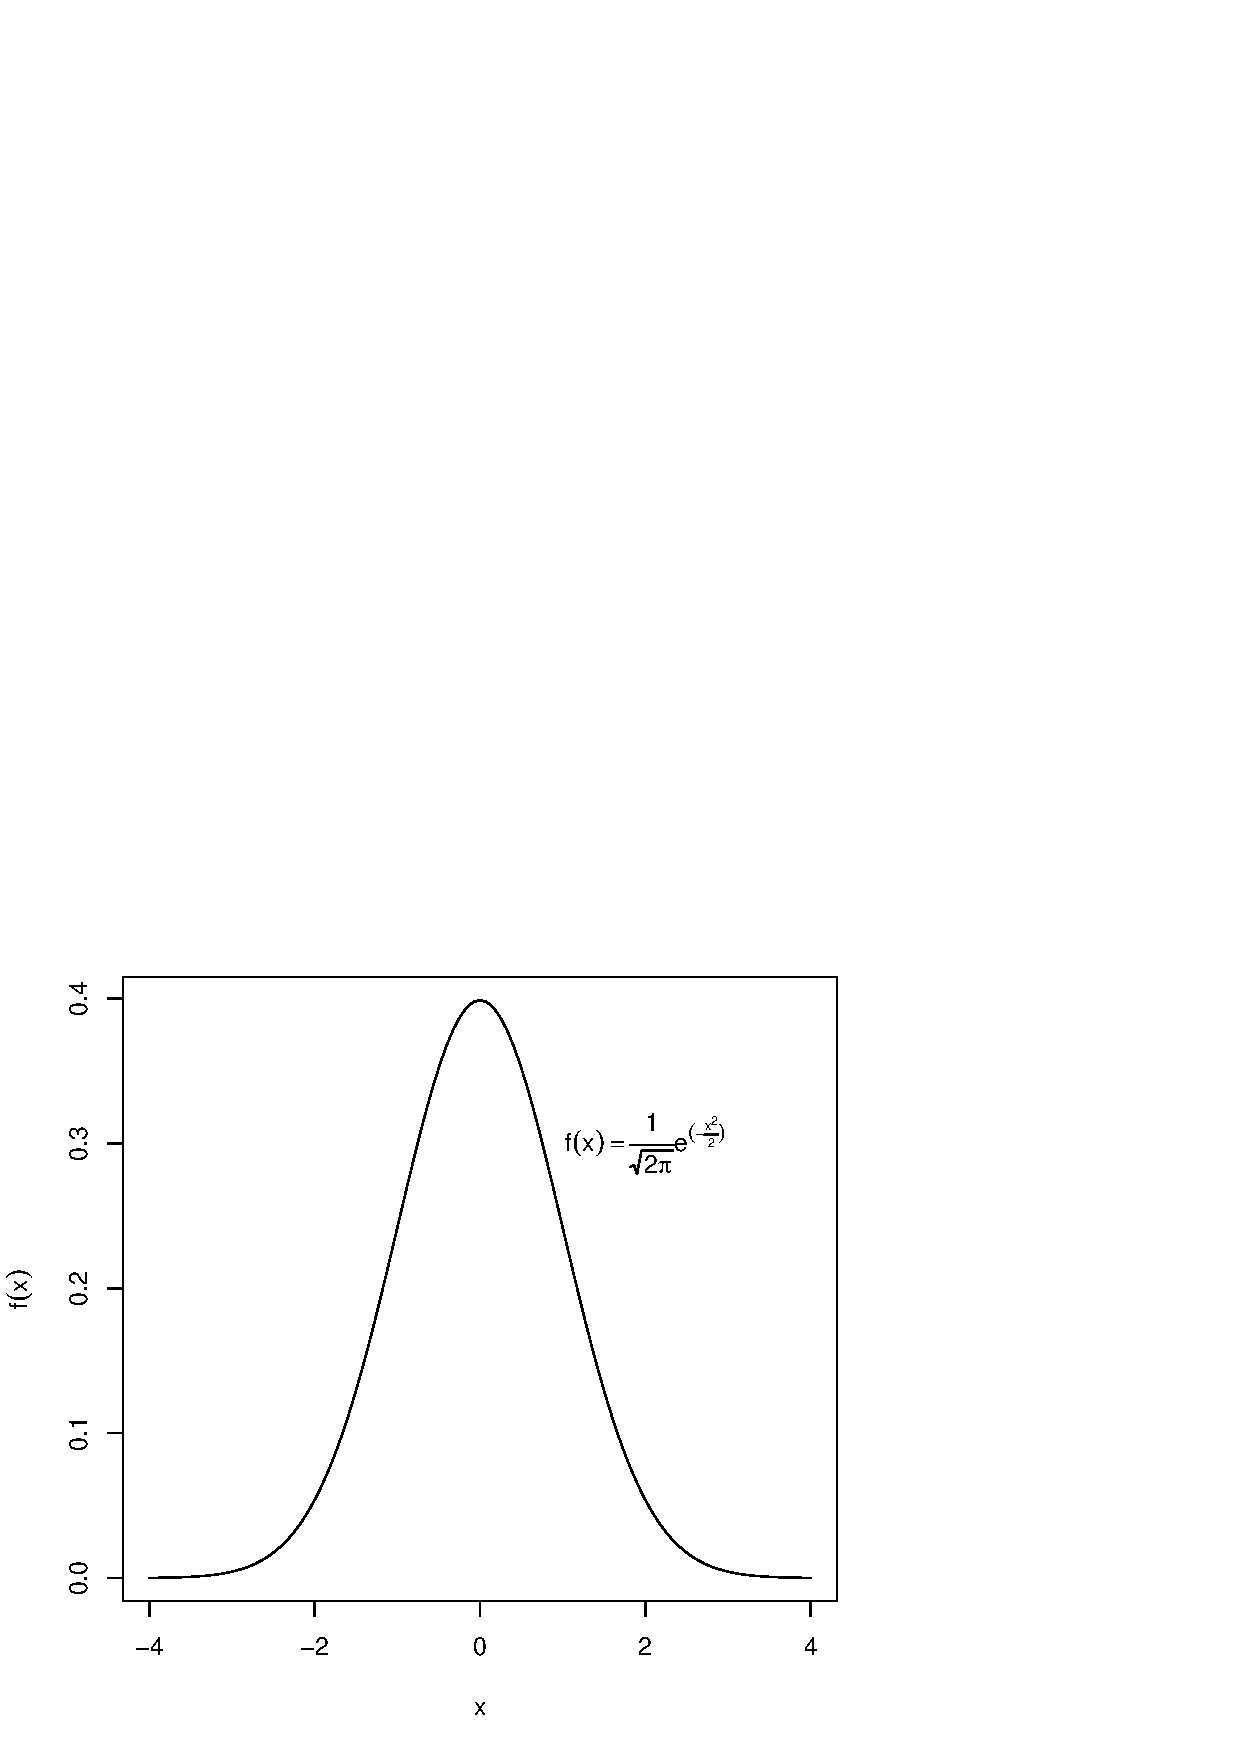
\includegraphics{./dibujos/02/-006}
\caption{Gráfica de la densidad gaussiana estándar}
\end{figure}
\end{center}
\end{frame}



\subsection{Variables absolutamente continuas}

\begin{frame}
\frametitle{Variables absolutamente continuas}
\begin{itemize}
\item Diremos que una v.a. tiene una ley \textbf{absolutamente continua} si su función de distribución se puede
escribir como 

$$\displaystyle F(x)=\int_{-\infty}^x f_{X}(t) dt$$ 

para todo $x\in\RR$.
\item  Donde $f$ es una función de densidad a la que llamaremos
función de densidad de la v.a. $X$
\item Cometeremos el abuso de decir \textbf{continua} una variable \textbf{absolutamente continua}.
\end{itemize}
\end{frame}

\begin{frame}
\frametitle{Propiedad}
Si $X$  es una v.a. tiene una función de distribución $F$ absolutamente continua se cumple que:
\begin{enumerate}[a)]
\item $F_{X}$ es continua.
\item Su funci\'on de densidad es $f(x)=F'_{X}(x)=\frac{d}{dx}F_{X}(x)$.
\item $D_X=\{x| f(x)>0\}$. Además $1=\int_{-\infty}^{\infty} f(x) dx=\int_{D_x} f(x) dx$.
\item Si  $A$ es un intervalo real, entonces $\displaystyle P(X\in A)=\int_{A} f(x) dx$.\newline
Por ejemplo si $A=(a,b]$ entonces 
$$\displaystyle P(X\in(a,b])=P(a<X\leq b)=\int_{a}^b f(x) dx.$$
\item Esta propiedad es similar para otro tipo de intervalos. 
\end{enumerate}
\end{frame}


\begin{frame}
\frametitle{Ejemplo}
\begin{itemize}
\item Supongamos que elegimos con ``equiprobabilidad'' un número al azar del intervalo real $(0,1)$.
\item Sea $X$ la v.a. que nos da ese número. 
\item Dado $0<x<1$ tenemos que 

$$P(X\leq x)=\frac{\mbox{longitud casos favorables}}{\mbox{longitud casos posibles}}= \frac{x-0}{1-0}=x.$$
\item Por lo tanto la función de distribución es 
$$F(x)=\left\{\begin{array}{ll} 0 &\mbox{ si } x\leq 0 \\
x  & \mbox{ si } 0<x<1\\
1 & \mbox{ si } x\geq 1
 \end{array}\right.
$$
\end{itemize}
\end{frame}

\begin{frame}
\begin{itemize}
\item La v.a. $X$  es absolutamente continua. Su función de densidad es 

$$
F'(x)=f(x)=\left\{\begin{array}{ll} 1 &\mbox{ si } 0 <x<1 \\
0 & \mbox{ en el resto de casos } 
 \end{array}\right.
$$

\item Ahora tenemos que  dado $0<x<1$

$$F(x)=\int_{-\infty}^x 1 dt =\int_{-\infty}^0 1 dt + \int_{0}^x t dt = \left.t\right|_{t=0}^{t=x}=x-0=x.$$
\item Efectivamente la integral de la función de densidad es la función de distribución.
\end{itemize}
\end{frame}

\begin{frame}
\frametitle{Ejemplo}

Sea $X$ una variable aleatoria con dominio $D_X=(1,2)$. Su función de densidad es:

$$f_X(x)=\left\{\begin{array}{ll}
k\cdot x^2+\frac{1}{3} & \mbox{ si } 0<x<1\\
0 & \mbox{en otro caso}
\end{array}\right.$$

Donde $k$ es una constante real ¿Cuál es el valor de $k$?

$1=\int_{0}^1 (k x^2+\frac{1}{3}) dx= \left.\left(k\frac{x^3}{3}+\frac{1}{3}x\right)\right|_{x=0}^{x=1}=
\left(k\frac{1}{3}+\frac{1}{3}\right)-(0+0)=\frac{k+1}{3}$

Resolviendo la ecuación  $1=\frac{k+1}{3}$ obtenemos que $k=2$.
\end{frame}

\begin{frame}
\frametitle{Gráfica de la función de densidad}
\begin{figure}
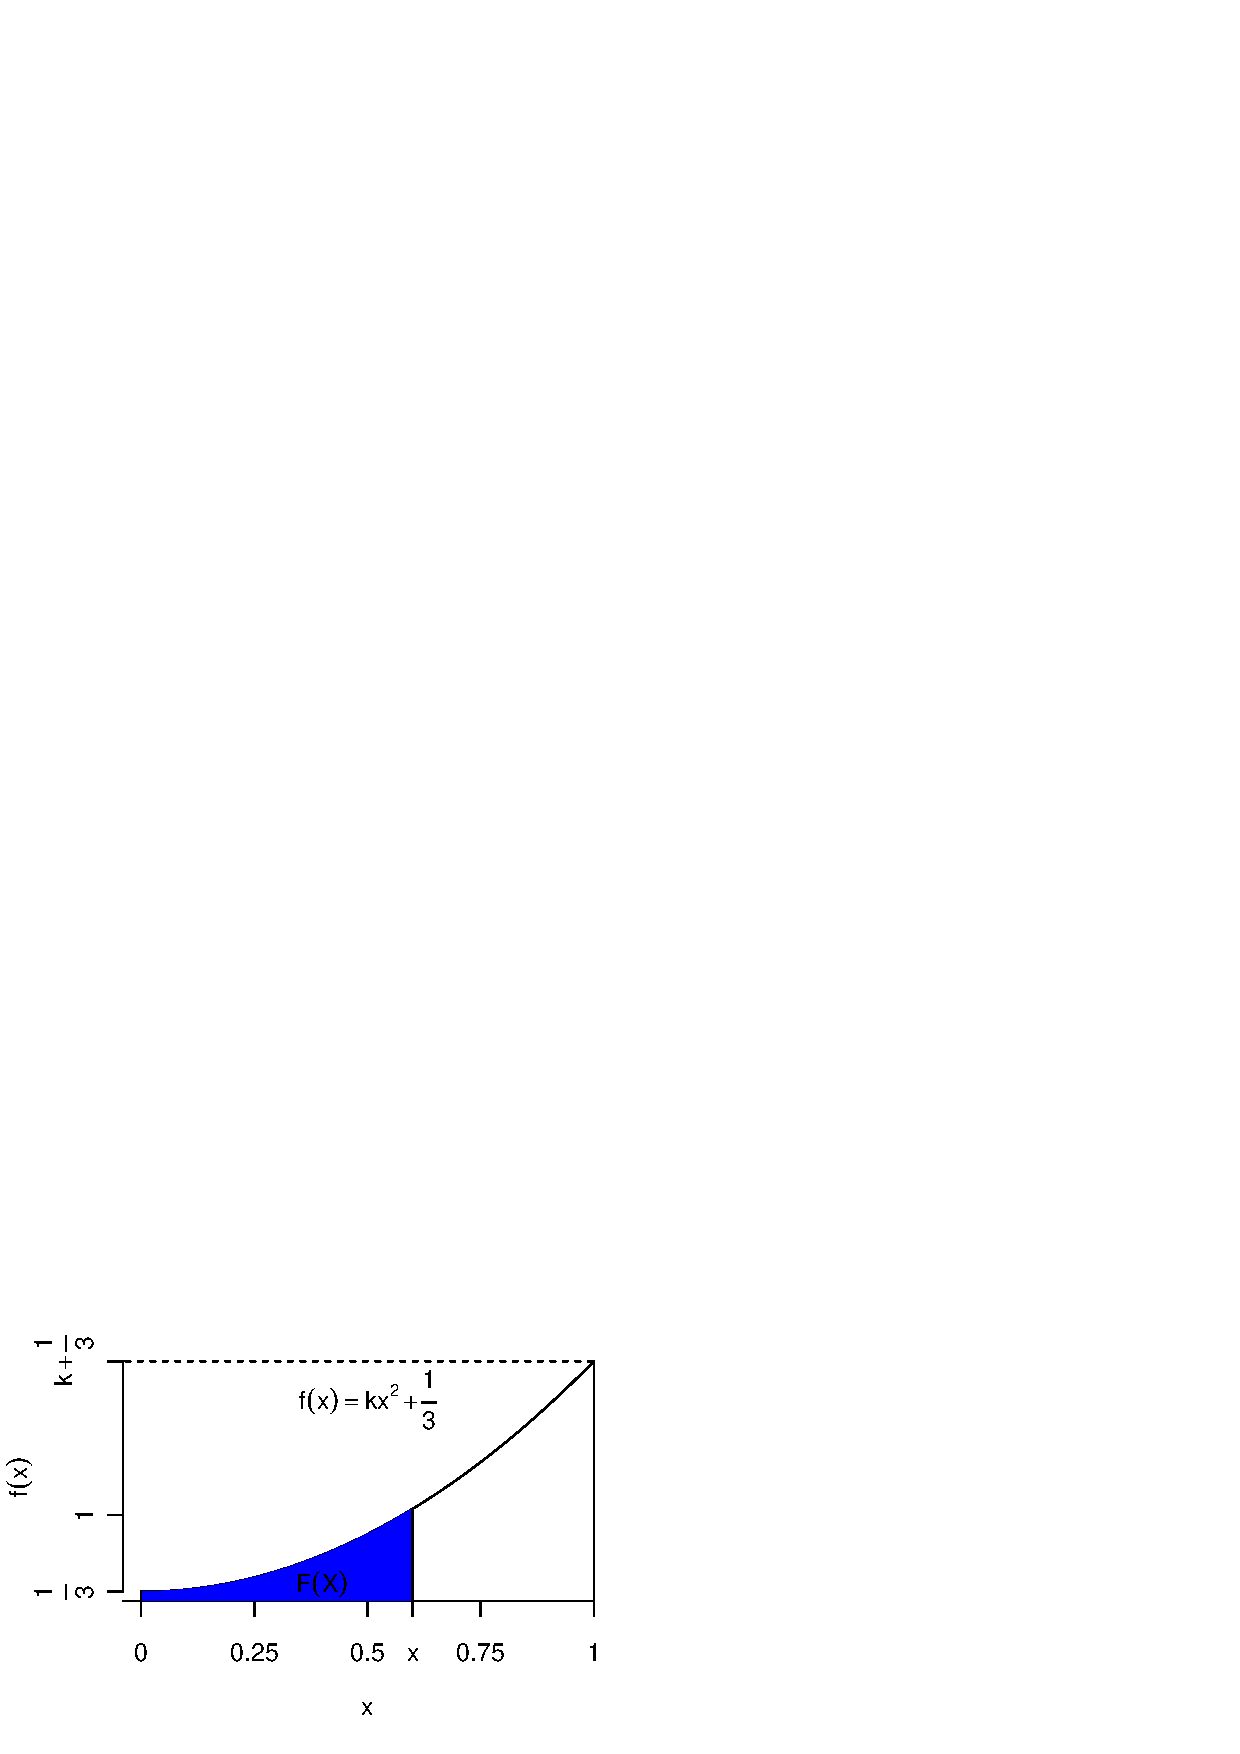
\includegraphics{./dibujos/02/-007}
\caption{Gráfica de una densidad y su  relación con la función de distribución.}
\end{figure}
\end{frame}

\begin{frame}
\begin{itemize}
\item En resumen,la función de densidad de la v.a. $X$ es 
$$f_X(x)=\left\{\begin{array}{ll}
2 x^2+\frac{1}{3} & \mbox{ si } 0<x<1\\
0 & \mbox{en otro caso}
\end{array}\right.$$
\item Dado $0<x<1$. la función de distribución es,

$F(x)=\int_{0}^x (2 t^2+\frac{1}{3}) dt =  \left.\left(2\frac{t^3}{3}+\frac{1}{3}t\right)\right|_{t=0}^{t=x}=
\left(2\frac{x^3}{3}+\frac{1}{3}x\right)=\frac{2 x^3+x}{3}.$
\end{itemize}
\end{frame}

\subsection{Esperanza y varianza para variables aleatorias continuas}

\begin{frame}
\frametitle{Esperanza de una variable aleatoria continua}
Sea $X$ una v.a. continua con función de densidad $f(x)$.
\begin{itemize}
\item Llamaremos \textbf{esperanza, media o valor esperado}  de la v.a. $X$ a 

           $$E(X)=\int_{-\infty}^{\infty}x \cdot f_{X}(x) dx$$
\item Si el  dominio de $X$ es  $D_X=(a,b)$ entonces

 $$E(X)=\int_{a}^{b}x \cdot f_{X}(x) dx$$ 
\end{itemize}
\end{frame}

\begin{frame}
\frametitle{Ejemplo}
Consideremos la v.a. $X$  con función de densidad:

$$
f(x)=\left\{\begin{array}{ll} 2 x^2+\frac{1}{3} &\mbox{ si } 0 <x<1 \\
0 & \mbox{ en el resto de casos } 
 \end{array}\right.
$$


Su valor esperado es 

\[
\begin{array}{rl}
E(X)= & \int_{0}^1 x \left(2 x^2 +\frac{1}{3}\right) dx= \int_{0}^1 \left(2 x^3 +\frac{1}{3}x\right) dx=
\left.\left(2 \frac{x^4}{4}+\frac{1}{3} \frac{x^2}{2}\right)\right|_{x=0}^{x=1} \\ = & \frac{1}{2}+\frac{1}{6}-(0+0)=\frac{2}{3}.
\end{array}
\]

\end{frame}




\begin{frame}
\frametitle{Esperanza de una función de una v.a.}
\begin{itemize}
\item  Sea $X$ una v.a. continua con densidad $f(x)$ y sea  $Y=g(X)$ una v.a. continua funci\'on de $X$. Entonces se define la \textbf{esperanza de la función} como :

$E(Y)=E(g(X))=\int_{-\infty}^{+\infty} g(x) f(x)dx$.
\item  Si el dominio de $X$ es $D_X=(a,b)$ entonces:
$E(Y)=E(g(X))=\int_{a}^{b} g(x) f(x)dx$.
\end{itemize}
\end{frame}


\begin{frame}
\frametitle{Ejemplo}
Consideremos la v.a. $X$  con función de densidad:

$$
f(x)=\left\{\begin{array}{ll} 2 x^2+\frac{1}{3} &\mbox{ si } 0 <x<1 \\
0 & \mbox{ en el resto de casos } 
 \end{array}\right.
$$


El valor esperado de la función $Y=X^2$ es:  

\[
\begin{array}{rl}
E(Y)= & E(X^2)=\int_{0}^1 x^2 \left(2 x^2 +\frac{1}{3}\right) dx= \int_{0}^1 \left(2 x^4 +\frac{1}{3}x^2\right) dx \\ = & 
\left.\left(2 \frac{x^5}{5}+\frac{1}{3} \frac{x^3}{3}\right)\right|_{x=0}^{x=1}=\frac{2}{5}+\frac{1}{9}-(0+0)=\frac{23}{45}.
\end{array}
\]

\end{frame}


\begin{frame}
\frametitle{Varianza de una v.a. continua}

Al igual que en el caso discreto, se define la \textbf{varianza} de una variable aleatoria continua como:

$$Var(X)=E(X-E(X)^2)$$

Se cumple que 

$$Var(X)=E(X^2)-E(X)^2$$

\end{frame}

\begin{frame}
\frametitle{Ejemplo}
Consideremos la v.a. $X$  con función de densidad:

$$
f(x)=\left\{\begin{array}{ll} 2 x^2+\frac{1}{3} &\mbox{ si } 0 <x<1 \\
0 & \mbox{ en el resto de casos } 
 \end{array}\right.
$$

Hemos visto anteriormente que $E(X)=\frac{2}{3}$ y $E(X^2)=\frac{23}{45}$. Por lo tanto su varianza es:

\[
Var(X)=E(X^2)-E(X)^2= \frac{23}{45}-\left(\frac{2}{3}\right)^2=\frac{1}{15}.
\]
\end{frame}


\begin{frame}
 \frametitle{Notaciones esperanzas y varianzas}
\begin{itemize}
\item De forma frecuente se denota por $\mu$ y $\sigma^2$ a la esperanza y varianza poblacionales de una distribución.
\item  La raíz cuadrada positiva de la varianza se denota por $\sigma$ y recibe el nombre de desviación típica poblacional.
\end{itemize}
\end{frame}

 \begin{frame}
\frametitle{Propiedades de la esperanza y la varianza}
\begin{enumerate}[a)]
\item $E(cte.)=cte$.
\item $E(a X+b)=a E(X)+b$.
\item $\displaystyle  E\left(\sum_{k=1}^{n }g_{k}(X)\right)=\sum_{k=1}^{n }E\left(g_{k}(X)\right)$.
\item Si $a<X<b$ entonces $a<E(X)<b$.
\item Si $X$ es una v.a. no negativa entonces $E(X)\geq 0$.
\item Si $g(X)\leq h(X)$ entonces $E(g(X))\leq E(h(X))$.
\item $Var(aX+b)=a^2 Var(X)$ donde $a,b$ son ctes. reales.
\item $Var(cte.)=0$
\end{enumerate}
\end{frame}

\section{Algunas modelos de distribuciones continuas}

\begin{frame}
\frametitle{Algunos  distribuciones continuas notables}
\begin{itemize}
\item En esta sección describiremos tres modelos de variables continuas.
\item Concretamente son: el modelo \textbf{uniforme}, el \textbf{exponencial} y el \textbf{gaussiano} o \textbf{normal}.
\item  A lo largo del curso, en la medida que sea necesario, expondremos otros modelos de distribuciones continuas como: la $t$ de \textbf{Student}, la \textbf{ji-cuadrado}, la $F$ de \textbf{Fisher}....
\item La función de distribución de estas distribuciones puede que no tenga una fórmula explícita.
\item En caso de no tener fórmulas explícitas se calcularan mediante tablas y usando \texttt{R}.
\end{itemize}
\end{frame}

\subsection{Distribución uniforme en el intervalo (a,b)}

\begin{frame}
\frametitle{Distribución uniforme}
 Una v.a. continua $X$ diremos que tiene una \textbf{distribución uniforme} sobre el intervalo real
$(a,b)$ ,$(a<b)$, si su función de densidad es
 $$f_X(x)=\left\{\begin{array}{ll}
\frac{1}{b-a} & \mbox{si } a<x<b\\ 0  & \mbox{en cualquier otro caso}
\end{array}
\right. $$ 
(como ejercicio comprobar que el área comprendida entre $f_X$ y el eje de abscisas (eje horizontal o eje~$X$)
vale~$1$.)

Si $X$ es una v.a. uniforme en el intervalo $(a,b),$ escribiremos $X\equiv U(a,b)$.

\end{frame}

\begin{frame}
Su función de distribución es:

$$F_X(x)=\left\{\begin{array}{ll} 0  & \mbox{si } x\leq a\\
\frac{x-a}{b-a} & \mbox{si } a<x<b\\ 1  & \mbox{si } b\leq x
\end{array}
\right. $$

Efectivamente:

\begin{itemize}
    \item Si $x\leq a$ entonces $F_X(x)=\int_{-\infty}^{x} f(t) dt= \int_{-\infty}^{x}
    0 dt =0$
    \item Si $a<x<b$ entonces $F_X(x)=\int_{-\infty}^{x} f(t) dt= \int_{-\infty}^{a}
    0 dt+\int_{a}^{x} \frac{1}{b-a} dt= 
    \frac{t}{b-a}\mid_{a}^{x}=\frac{x}{b-a}-\frac{a}{b-a}=\frac{x-a}{b-a}$
    \item  Por último si $x\geq b$ entonces $F_X(x)=\int_{-\infty}^{x} f(t)
    dt=1$ (ejercicio).
\end{itemize}
\end{frame}

\subsubsection{Esperanza y varianza  para $U(a,b)$}
\begin{frame}
\frametitle{Esperanza y varianza  para  una v.a. $X$ con distribución  $U(a,b)$}
\[
\begin{array}{rl}
E(X)= & \int_{-\infty}^{+\infty} x f_X(x) dx=\int_{a}^{b} x \frac{1}{b-a} dx =
\frac{x^2}{2(b-a)}\mid _{a}^{b}=\frac{b+a}{2}, \\ & \\
E(X^2)= & \int_{-\infty}^{+\infty} x^2 f_X(x) dx=\int_{a}^{b} x^2 \frac{1}{b-a}
dx =\frac{x^3}{3(b-a)}\mid_{a}^{b} =\frac{b^3-a^3}{3(b-a)} \\ = & \frac{b^2+ab+a^2}{3}, \\ & \\
Var(X)= & E(X^2)-(E(X))^2=\frac{b^2+ab+a^2}{3}-(\frac{b+a}{2})^2=\frac{(b-a)^2}{12}.
\end{array}
\]
\end{frame}

\begin{frame}
\frametitle{Gráfica de la distribución $U(-1,2)$}
\begin{figure}[h]
\begin{center}
\scalebox{0.6}[0.6]{
\begin{tabular}{cc}       
\includegraphics[scale=0.5]{densidaduniforme12}
&
\includegraphics[scale=0.5]{distribucionuniforme12}\\
 a) & b) 
\end{tabular}
}
\end{center}
\caption{ Gráficas de la función de densidad (a)  y de la función de distribución (b) de una v.a. $U(-1,2)$.}
\end{figure}
\end{frame}

\subsubsection{Resumen v.a con distribución uniforme, $U(a,b)$}

\begin{frame}
\scalebox{0.8}[0.8]{
\begin{tabular}{|c|c|c|c|c|}
\hline \begin{tabular}{c} Valores\\ admisibles.\end{tabular} & $f_{X}(x)$ & $F_X(x)=P(X\leq
X)=$ &
 $E(X)$ & $Var(X)$\\\hline & & & &\\
 $D_X=(a,b)$ & $\left\{\begin{array}{ll}
\frac{1}{b-a} & \mbox{si } a<x<b\\ 0  & \mbox{en cualquier otro caso}
\end{array}
\right.$  &  $\left\{\begin{array}{ll} 0 & \mbox{ si } x\leq a\\
          \frac{x-a}{b-a} & \mbox{ si } a\leq x\leq\\
          1 & \mbox{ si } b\leq x\end{array}\right.$
 & $\frac{a+b}{2}$ & $\frac{(b-a)^2}{12}$ \\& & & &\\ \hline
\end{tabular}
}
\end{frame}
\subsection{Distribución exponencial (exponencial negativa)}
\begin{frame}

\frametitle{Modelo exponencial}

\begin{itemize}
\item      Supongamos que tenemos un proceso Poisson con parámetro $\lambda$ en una unidad de tiempo.
\item    Entonces dadas $t$ unidades de tiempo tenemos que $X_{t}=$ número de eventos en el intervalo de tiempo $(0,t]$ es una $Po(\lambda\cdot t)$. 
\item Consideremos la v.a. $T=$tiempo transcurrido entre dos eventos Poisson consecutivos.
\item Dado $t>0$, tenemos que 
$P(T>t)=P(\mbox{Cero eventos en el intervalo}(0,t])=P(X_{t}=0)= $
$\frac{(\lambda t)^0}{0!} e^{-\lambda t}=e^{-\lambda t}.$
\end{itemize}
\end{frame}

\begin{frame}
\begin{itemize}
\item   Tomando complementarios, la función de distribución de $T$ será

         $$F_{T}(t)=P(T\leq t)=\left\{\begin{array}{ll} 0 &\mbox{ si } t\leq 0\\
          1-P(T>t)=1-e^{-\lambda t}& \mbox{ si } t>0\end{array}\right.$$
\item Por lo tanto
         $$f_{T}(t)=\left\{\begin{array}{ll}
         \lambda e^{-\lambda t} & \mbox{ si }  t>0\\
         0 & \mbox{ si } t\leq 0
         \end{array}\right.$$
\item Ésta es la distribución exponencial y la denotaremos por $Exp(\lambda)$
\end{itemize}
\end{frame}

\begin{frame}
\frametitle{Propiedad de la falta de memoria}
Sea $X$  una v.a. $Exp(\lambda)$ entonces

          $$P(X>s+t/X>s)=P(X>t)\mbox{  para todo } s,t\in \RR$$

          Toda v.a. absolutamente continua, que tome valores positivos
          y que verifique la propiedad de la falta de memoria es una v.a.
          exponencial.
\end{frame}


\subsubsection{Resumen v.a con distribución exponencial, $Exp(\lambda)$}

\begin{frame}

Sea $X\equiv Exp(\lambda).$

%\begin{center}ç
\scalebox{0.7}[0.7]{
\begin{tabular}{|c|c|c|c|c|}
\hline \begin{tabular}{c} Valores\\ admisibles.\end{tabular} & $f_{X}(x)$ & $F_X(x)=P(X\leq
X)=$ &
 $E(X)$ & $Var(X)$\\\hline & & & &\\
 $D_X=(0,+\infty)$ & $\left\{\begin{array}{ll}
         \lambda e^{-\lambda x} & \mbox{ si }  x>0\\
         0 & \mbox{ si } x\leq 0
         \end{array}\right.$ &  $F_{X}(x)=P(X\leq x)=\left\{\begin{array}{ll} 0 &\mbox{si } x\leq 0\\
          1-e^{-\lambda x}& \mbox{si } x>0\end{array}\right.
$ & $\frac{1}{\lambda}$ & $\frac{1}{\lambda^2}$ \\& & & &\\ \hline
\end{tabular}
%\end{center}
}
\end{frame}
%\end{document}
\subsection{Distibución normal o gaussiana}

\begin{frame}
\frametitle{Distribución normal o Gaussiana}
Diremos que una v.a. $X$ sigue una \textbf{ley normal} o \textbf{gaussiana} de parámetros $\mu$ y $\sigma$ y lo denotaremos por $N(\mu,\sigma)$ si tiene por funci\'on de densidad:

$$f_{X}(x)=\frac{1}{\sqrt{2\pi}\sigma} e^{\frac{-(x-\mu)^2}{2\sigma^{2}}} \mbox{ para todo } x\in \RR$$

La gráfica de esta función es la conocida campana de Gauss, que ya hemos dibujado dos veces.  La v.a. normal con $\mu=0$ y $\sigma=1$ recibe el
nombre de normal est\'andard. 

La normal estándard se suele denotar por la letra $Z$ y su función de distribución $F_Z$.
\end{frame}

\begin{frame}
\frametitle{Propiedades} 
Sea $X$ una v.a. $N(\mu,\sigma^2)$ y sea $f_{X}$ su funci\'on de densidad. Entonces:
\begin{enumerate}[a)]
\item Evidentemente $f_{X}$ verifica todas las propiedades de las funciones de densidad.
\item $f_{X}(\mu-x)=f_{X}(\mu+x)$ es simétrica respecto de la recta $x=\mu$
\item $f_{X}$ alcanza el máximo en $x=\mu$
\item Si $F_{X}$ la función de distribución de $X$ entonces  $F_{X}(\mu+x)=1-F_{X}(\mu-x)$. En particular si $Z$ es una $N(0,1)$ entonces $F_{Z}(-x)=1-F_{Z}(x)$
\item $Z=\frac{X-\mu}{\sigma}$ es una v.a. $N(0,1)$ y $X=\sigma Z+\mu$ es una $N(\mu,\sigma^{2})$ donde $Z$ es la normal estándar.
\end{enumerate}
\end{frame}


%%%%%aqui
\begin{frame}
\frametitle{Importancia  y propiedades de la distribución normal}
\begin{itemize}
\item  La variable aleatoria normal es una de las más importantes de la estadística.
\item  La justificación es que la distribución de muchos estadísticos como la media o la proporción muestral se aproximan  a una distribución normal cuando los tamaños de las muestras son grandes.
\item 
Como ya hemos visto en distribuciones continuas las probabilidades se calculan como áreas que se forman debajo de una curva, llamada curva de densidad, y el eje horizontal.
 \item  Como en todas las distribuciones continuas la probabilidad $P(X\leq x)$. es el área comprendida entre el eje horizontal la curva normal y la vertical que corta al eje horizontal en $x$, ver la fig.~\ref{areacurvanormalgeneralderecha}.
\end{itemize}
\end{frame}
 
\begin{frame}[fragile]
\begin{figure}[htbp]
\begin{center}
%\includegraphics{areacurvanormalgeneralderecha.eps}
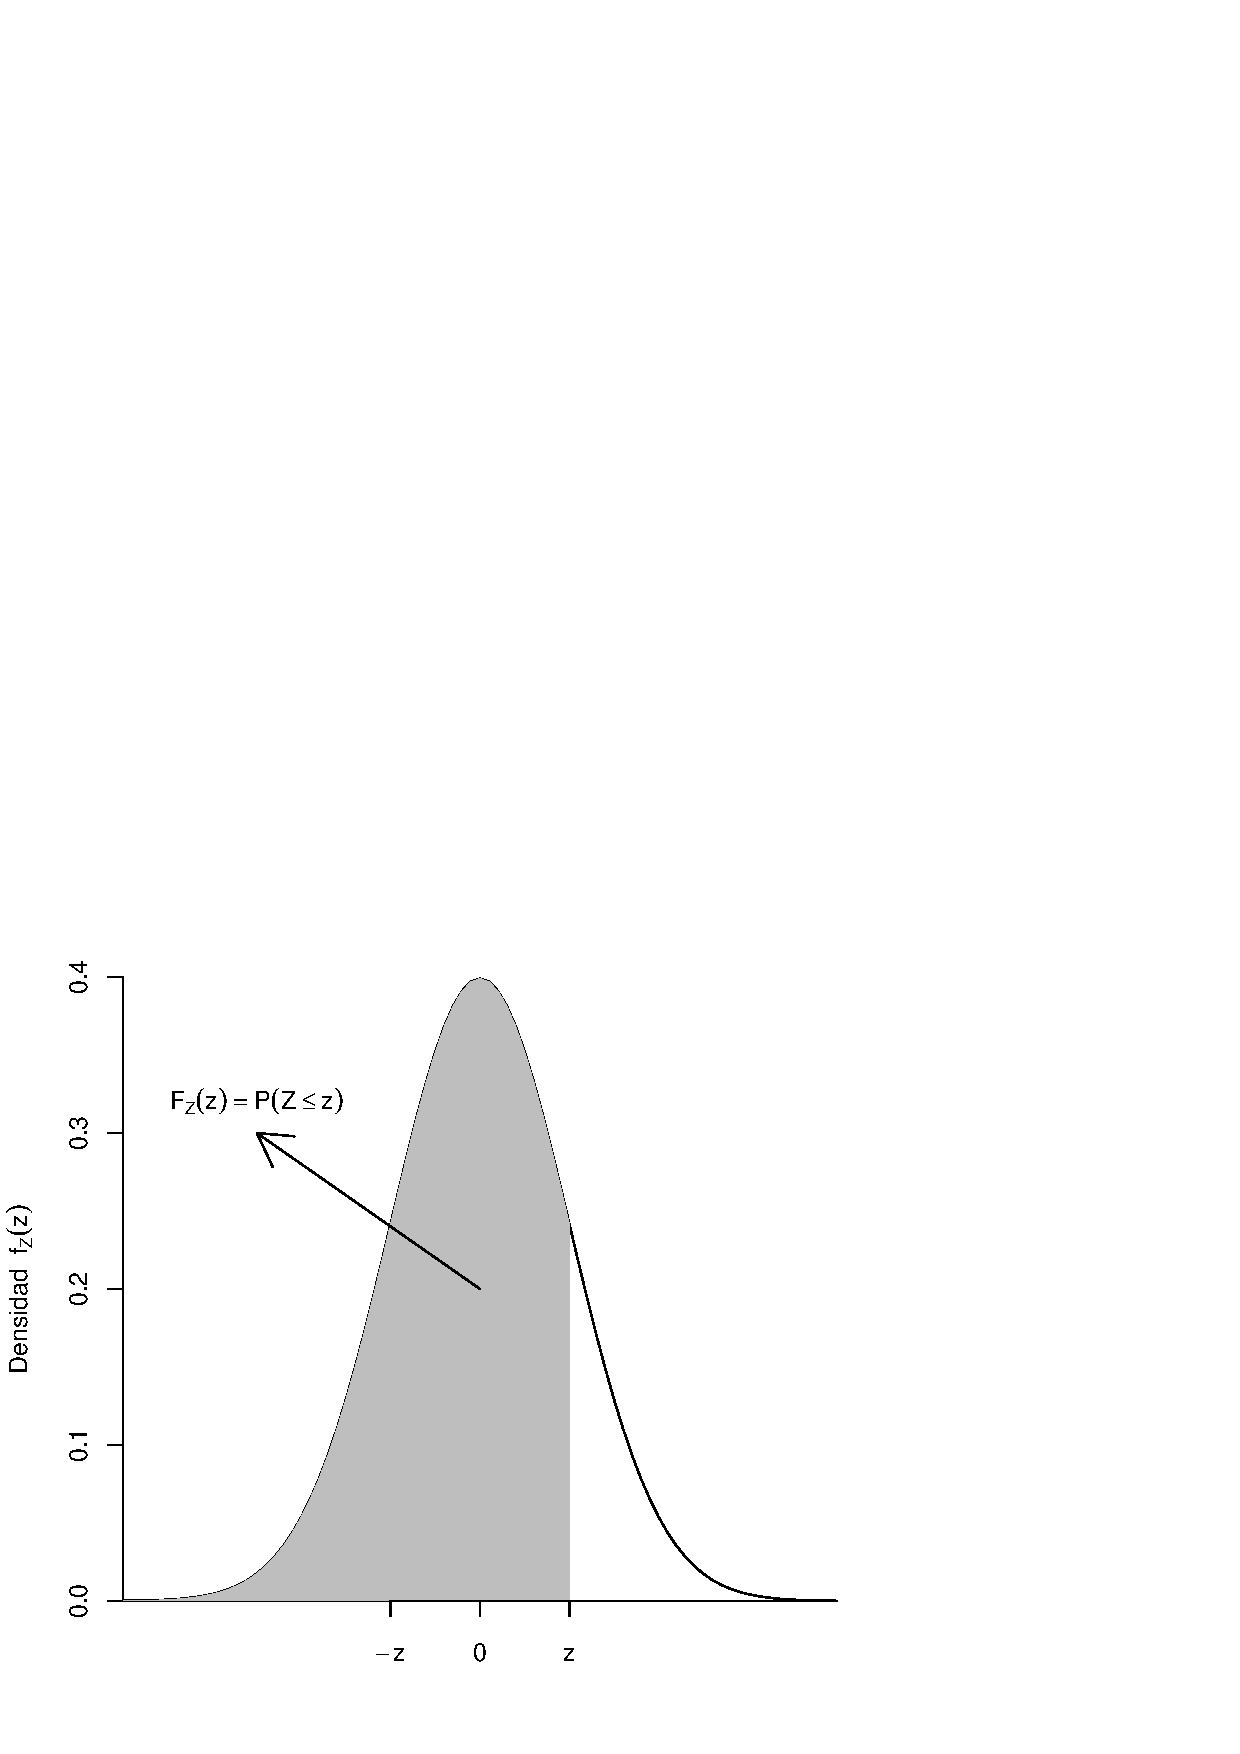
\includegraphics{./dibujos/02/-008}

\end{center}
\caption{la $P(X\leq x)$ como un área bajo la curva normal.}
	\label{areacurvanormalgeneralderecha}
\end{figure}
\end{frame}
 
 \subsubsection{Comportamiento de la curva normal}
\begin{frame}
\begin{itemize}
\item  La curva normal toma distintas formas en función del valor de sus pa\-rá\-me\-tros.
\item  Consideremos dos curvas normales con medias $\mu_1=\mu_2$ respectivamente y varianzas $\sigma_1^2<\sigma_2^2$.
\item  Las dos curvas estarán centradas en la media, pero la segunda será más achatada, pues tiene varianza mayor y los valores se alejan más  del valor medio.
\item  Este caso se ilustra en la fig.~\ref{dosnormalesmediasigualesvardistintas}
 \end{itemize}
\end{frame}

\begin{frame}
 
 \begin{center}
\begin{figure}[htbp]
	\includegraphics{dosnormalesmediasigualesvardistintas.png}
	\caption{Dos curvas normales $X_1$ y $X_2$ con $\mu_1=\mu_2$ y $\sigma_1^2<\sigma_2^2$.}
	\label{dosnormalesmediasigualesvardistintas}
\end{figure}
\end{center}
\end{frame}

\begin{frame}

En el caso en que las varianzas sean iguales y las medias distintas, las curvas normales tienen la misma forma pero cada una de ellas está centrada en cada una de sus medias. El efecto puede verse en la fig.~\ref{dosnormalesmediasdistintasvariguales}



\begin{center}
\begin{figure}[htbp]
	\includegraphics{dosnormalesmediasdistintasvariguales.png}
	\caption{Dos curvas normales $X_1$ y $X_2$ con $\mu_1<\mu_2$ y $\sigma_1^2=\sigma_2^2$.}
	\label{dosnormalesmediasdistintasvariguales}
\end{figure}
\end{center}
\end{frame}
\begin{frame}
Por último si las medias son distintas y las varianza también se obtienen curvas como las de la fig.~\ref{dosnormalesmediasdistintasvardistintas}

 \begin{center}
\begin{figure}[htbp]
	\includegraphics[scale=0.8]{dosnormalesmediasdistintasvardistintas.png}
	\caption{Dos curvas normales $X_1$ y $X_2$ con $\mu_1<\mu_2$ y $\sigma_1^2<\sigma_2^2$.}
	\label{dosnormalesmediasdistintasvardistintas}
\end{figure}
\end{center}
\end{frame}




\subsubsection{Estandarización de la variable normal}
\begin{frame}
\frametitle{Estandarización de la variable normal}

\begin{itemize}
\item La estandarización o tipificación de una variable ya fue comentada en el primer tema.
\item  Consiste en transformar una variable o una serie de datos a unos datos típicos o estándars en el sentido que todos tengan esperanza o media $0$ y varianza poblacional o muestral igual a $1$. 
\item Para conseguir este efecto es suficiente restar a la variable la media y dividir el resultado por la desviación típica. Estas ideas ya se vieron en el módulo anterior.
\end{itemize}

\end{frame}
\begin{frame}
\begin{itemize}
\item En general supongamos que tenemos un variable $X$ con valor esperado $\mu$ y desviación típica $\sigma$. Entonces sus puntuaciónes estándar (\textit{$z$-scores}) se suele denotar por la letra $Z$ se calculan como $Z=\frac{X-\mu}{\sigma}$.
para la versión  poblacional
\item Mientras que para la versión muestral, como ya vimos, es $=\frac{x-\overline{x}}{s}$
\end{itemize}
\end{frame}

\begin{frame}
\begin{itemize}
\item La variable o serie de datos $Z$ tiene esperanza o media $0$ y varianza poblacional o muestral $1$. 
\item En este sentido es una variable de puntuaciones estándar y puede servirnos para comparar las puntuaciones de dos variables o series de datos
\item  Este es el motivo por el que recibe el nombre de estándar, pues reduce los datos o variables a ``\textsl{unidades estándar}". \item Existen otras  formas de reducir variables o series a puntuaciones que sean comparables. 
\end{itemize}
\end{frame}

\subsubsection{Estandarización de la variable normal}
\begin{frame}
\begin{itemize}
\item Para el caso de la variable aleatoria normal tenemos una propiedad importante. 
\item Es suficiente conocer todas las probabilidades de una variable aleatoria $Z$ normal estándar o típica es decir con $\mu=0$ y $\sigma=1$ para conocer las probabilidades de cualquier variable normal de media $\mu$ y desviación típica $\sigma$.
\item  La igualdad que relaciona estas dos probabilidades es
$$P(X\leq x)=P(Z\leq \frac{x-\mu}{\sigma}).$$
Donde $Z$ es una variable que sigue la ley normal estándar, es decir una normal con $\mu=0$ y $\sigma=1$.
\item Lo que nos dice esta propiedad es que cuando $X$ es una variable aleatoria con distribución normal de parámetros $\mu$ y $\sigma^2$, la variable $Z=\frac{X-\mu}{\sigma}$ sigue una distribución normal estándar.
\item A la función que nos da las probabilidades de la variable normal estándar $Z$  la denotaremos por $F_Z(z)=P(Z\leq z).$
\end{itemize}
\end{frame}

\begin{frame}

Es sencillo comprender mirando la fig.~\ref{areanormalestandarderecha} que la función de distribución de la variable normal estándar cumple la propiedad: $F_Z(-z)=1-F_Z(z).$

 \begin{center}
\begin{figure}[htbp]
	%\includegraphics[scale=0.8]{areanormalestandarderecha.pdf}
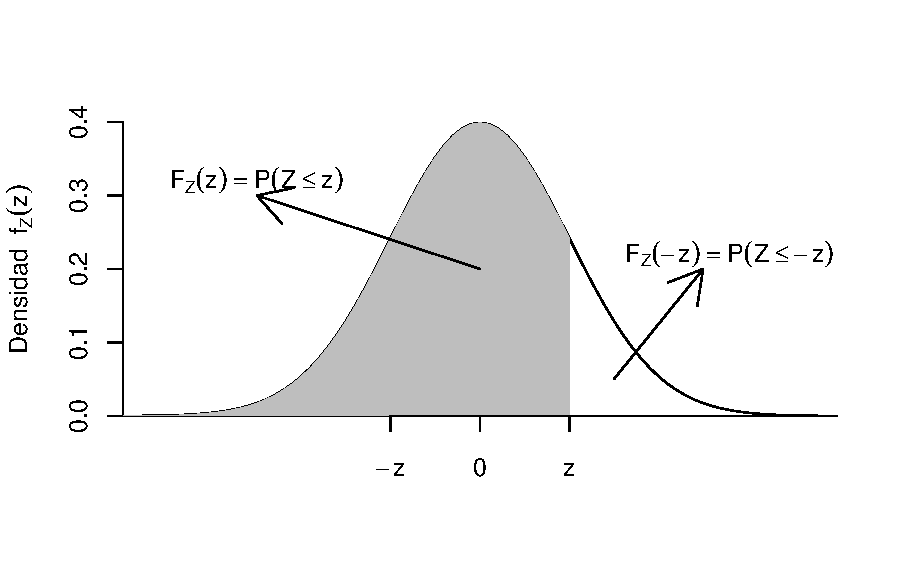
\includegraphics{./dibujos/02/-009}

\caption{Justificación gráfica de la propiedad de la normal estándar: $F_Z(-z)=1-F_Z(z)$.}
	\label{areanormalestandarderecha}
\end{figure}
\end{center}

\end{frame}


\begin{frame}

\subsubsection{Uso de tablas para el cálculo de la función de distribución normal.}
\begin{itemize}
\item Las  tablas para el cáculo de la normal están disponibles  en ``http://bioinfo.uib.es/\~{}recerca/mates2/tablasDistribuciones/''.
\item Estas tablas contienen los valores de la distribución normal estándar. Es decir los valores de  $F_{Z}(z)=P(Z\leq z)$ para una variable
$Z$ normal estándar.
\item  La primera tabula los valores negativos y la segunda, los positivos. Por ejemplo $F_{Z}(1.78)=0.9625$, es un resultado que se encuentra en la
segunda tabla. Si queremos saber el valor de $F_Z(-1.78)=1-F_Z(1.78)=0.0375$ donde hemos utilizado la propiedad $F_Z(-z)=1-F_Z(z)$.
\item La entrada horizontal de la tabla es el segundo decimal del número que buscamos, mientras que la primera columna contiene las unidades y el
primer decimal.
\item Si queremos calcular la probabilidad de que $Z$ esté comprendida entre $-2$ y $2$ 
\item $P(-2\leq Z\leq 2)=F_Z(2)-F_Z(-2)=0.9772-0.0228=0.9544.$
\end{itemize}
\end{frame}

\begin{frame}
\begin{itemize}
\item La explicación es la siguiente: la probabilidad de que $Z$ esté entre $-2$ y $2$ es el área comprendida bajo la curva normal, el eje horizontal
y las verticales que pasa por $-2$ y $2$.
\item  Este área es el área encerrada bajo la curva y  menor o igual que~$2$ menos el área encerrada bajo la curva y menor que~$-2$.
\item En general se tiene que 
$P(a\leq Z\leq b)=P(Z\leq a)-P(Z\leq b)=F_Z(a)-F_Z(b).$
\item En particular dado $\delta>0$ entonces
$P(-\delta\leq Z \leq \delta)=F_{Z}(\delta)-F_{Z}(-\delta).$
\item \textbf{Nota:} En el caso de variables continua los $\leq$ se pueden cambiar por $<$ (uno todos o ninguno) y las probabilidades no varían. Es decir $P(Z\leq a)=P(Z< a)$.
\end{itemize}
\end{frame}

\begin{frame}

\frametitle{Ejemplo} 
Sea $Z$ una variable normal estándar. Utilizando las tablas de la distribución normal estándar calcular las siguientes probabilidades:
\begin{enumerate}[a)]
\item $P(0< Z < 3.99)=F_Z(3.99)-F_Z(0)\approx 1-0.5=0.5$. 
\item $P(-3.99\leq Z \leq 3.99)=F_{Z}(3.99)-F_{Z}(-3.99)\approx 1.$
\item $P(-3\leq Z \leq 3)=F_{Z}(3)-F_{Z}(-3)= 0.9987-0.0013=0.9974$.
\item $P(Z\leq -2)=F_Z(-2)=0.0228$.
\item $P( Z \leq 2)=F_{Z}(2)=0.9772$.
\item $P( Z \geq 2)=1-P(Z<2)=1-F_{Z}(2)=0.0228$.
\item $P( Z \geq -2)=1-P(Z< -2)=1-F_{Z}(-2)=1-(1-F_Z(2))=F_Z(2)$.
\item Dado $\delta>0$, $P(-\delta\leq Z \leq
\delta)=F_{Z}(\delta)-F_{Z}(-\delta)=F_Z(\delta)-(1-F_Z(\delta))=2\cdot  F_Z(\delta)-1$.
\item Utilizando la igualdad anterior
$P(-2\leq Z \leq 2)=2\cdot  F_Z(2)-1=2 \cdot 0.9772-1=0.9544$.
\end{enumerate}

\end{frame}


\begin{frame}

\begin{itemize}
\item No sólo podemos utilizar la tabla para calcular la probabilidad en un valor determinado. 
\item También la podemos utilizar para calcular los cuantiles de $Z$ que tienen la misma definición que vimos en estadística descriptiva.
\item  Por ejemplo si quiero calcular el valor $z$ tal que $P(Z\leq z)=0.9099$ buscamos dentro de la tabla el valor $0.9099$, o el más cercano, en este caso es $F_Z(1.34)=0.9099$ por lo tanto el valor buscado es $z=1.34$.
\end{itemize}
\end{frame}

\begin{frame}

\frametitle{Ejemplo}
 Calcular los valores que se piden para una variable $Z$ normal estándar.
\begin{enumerate}[a)]
\item Calcular el valor $z$ tal que $P(Z\leq z)=0.504$. Mirando las tablas se obtiene que  $F_Z(0.01)=0.504$ por lo tanto el valor pedido es $z=0.01$.
\item Calcular el valor $z$ tal que $P(Z> z)=0.9633$. Primero hacemos el complementario $P(Z>z)=1-P(Z<z)=1-F_Z(z)=0.9633$. Ahora despejando obtenemos que  el valor buscado cumple
que $F_Z(z)=1-0.9633= 0.0367$. Mirando dentro de las tablas se obtiene que $F_Z(-1.79)=0.0367$. En definitiva el valor buscado es $z=-1.79$
\end{enumerate}
\end{frame}



\begin{frame}
\frametitle{Cáculo de probabilidad de una v.a. $N(\mu,\sigma)$.}
\begin{itemize}
\item Sólo nos queda ver como calculamos las probabilidades de una variable aleatoria normal de media $\mu$ y varianza $\sigma^2$.
\item  Recordemos la relación básica que dice que la variable tipificada de una normal sigue una ley normal estándar. Si $X$ es una normal de media
$\mu=1$ y varianza $\sigma^2=4$ se tiene que 
$$Z=\frac{X-\mu}{\sigma}=\frac{X-1}{2}$$

sigue una ley  normal estándar.
\item Por lo tanto   $P(X\leq x)=F_Z(\frac{x-\mu}{\sigma})$.
\end{itemize}
\end{frame}

\begin{frame}
\frametitle{Ejemplo}
\begin{enumerate}[a)]
\item 
Por ejemplo $P(X\leq 2)=P(\frac{X-1}{2}\leq \frac{2-1}{2})=P(Z\leq \frac{1} {2})=F_Z(0.5)=0.6915$.
\item Si queremos calcular el cuantil $0.6915$ de la variable $X$ será aquel valor $X$ tal que $P(X\leq x)=0.6915$. Tipificamos la variable $X$

$$P(X\leq x)=P(\frac{X-1}{2}\leq \frac{x-1}{2})=P(Z\leq \frac{x-1} {2})=F_Z(\frac{x-1} {2})=0.6915 ,$$

mirando en las tabla de la normal estándar resulta que $F_Z(0.5)=0.6915$, entonces 

$$ \frac{x-1} {2}=0.5 ,$$

despejando $x$ de la ecuación anterior se obtiene que $x=2\cdot 0.5+1= 2$.
\end{enumerate}
\end{frame}
 
 
 
 \begin{frame}
\frametitle{Resumen propiedades de la normal}
Resumiendo podemos utilizar las siguientes propiedades, $X\equiv N(\mu,\sigma)$
    \begin{itemize}
    \item  $Z$ es su variable tipificada, es decir,
    $Z=\frac{X-\mu}{\sigma}\equiv N(0,1)$ entonces:

    $$P(X\leq x)=P(\frac{X-\mu}{\sigma}\leq
    \frac{x-\mu}{\sigma})=F_{Z}(\frac{x-\mu}{\sigma})$$

   \item  Cuando tengamos un intervalo
    $$P(a<X<b)=P(\frac{a-\mu}{\sigma}<\frac{X-\mu}{\sigma}<\frac{b-\mu}{\sigma})=$$

    $$=P(\frac{a-\mu}{\sigma}<Z<\frac{b-\mu}{\sigma})=F_{Z}(\frac{b-\mu}{\sigma})-
    F_{Z}(\frac{a-\mu}{\sigma})$$
    \item Si $\delta>0$ $P(\mu-\delta\leq X \leq
\mu+\delta)=2 F_Z(\frac{\delta}{\sigma})-1$
\end{itemize}
\end{frame}

\begin{frame}
\frametitle{Ejemplo}
Sea $X$ una normal com media $2$ y varianza $4$, entonces
    \begin{enumerate}[a)]
\item  $P(1< X< 2)= P(\frac{1-2}{2}<\frac{X-2}{2}<\frac{2-2}{2})=
    P(\frac{-1}{2}<Z<0)=F_{Z}(0)-F_{Z}(-0.5)=\frac{1}{2}-1+F_{Z}(0.5).$
    \item $P(X>3)=P(\frac{X-2}{2}>\frac{3-2}{2})=
    P(Z>0.5)=1-F_{Z}(0.5).$
    \end{enumerate}
\end{frame}


\begin{frame}
\frametitle{Aproximación de una Binomial por una distribución normal}
\begin{itemize}
\item  Bajo determinadas condiciones la distribución normal puede aproximar a la distribución binomial.
\item  Sea $X$ una v.a. con distribución $B(n,p)$ entonces $E(X)=np$  y $Var(X)=npq$.
\item Sea $Z=\frac{X-E(X)}{\sqrt{Var(X)}}=\frac{X-np}{\sqrt{np(1-p)}}$.
\item Si $n$ es grande y $p$ no está muy cercano a $0$ o a $1$ la distribución de $Z$ se aproxima a una normal estándar.
\item La aproximación se realiza de la siguiente manera
$P(X=k)\approx P\left({{k-0.5-np}\over \sqrt{npq}}\leq Z \leq {{k+0.5-np}\over
\sqrt{npq}}\right)$
\item Mediante un razonamiento similar : $$\ P(X\leq k)\approx P\left(Z \leq
{{k+0.5-np}\over \sqrt{npq}}\right)$$
\item Y también $\ P(a\leq X\leq b)\approx\approx P\left(\frac{a-0.5-np}{\sqrt{npq}}\leq Z \leq \frac{b+0.5-np}{\sqrt{npq}}\right)$
\item Donde, en todos los  casos $Z$ se toma como una normal estándar.
\end{itemize}
\end{frame}
%%%%%%s%%
%%%%%%%%\textbf{Criterio:} La aproximaci�n es fiables si $np(1-p)>9$ y $n\geq 20$ y $p$ pr�ximo a
%%%%%%%%0.5
\begin{frame}
\frametitle{Corrección de continuidad} 
\begin{itemize}
\item El motivo de sumar o restar 0.5 en las aproximaciones es
corregir el efecto que tienen aproximar una v.a. discreta por una continua.
\item Esta operación recibe el nombre de corrección de continuidad de Fisher. 
\item Gráficamente el área que hacemos
corresponder a la probabilidad de cada valor entero $k$ en una binomial corresponde a la
comprendida entre la curva normal y el  segmento centrado en $k$ de amplitud 1.
\end{itemize}
\end{frame}

\begin{frame}
\frametitle{Ejemplo}
    $X$=número de caras en 100 lanzamientos de una moneda.
    $P(\mbox{cara})=\frac{1}{2}$. Calcular:

    \begin{enumerate}[a)]
    \item $P(40\leq X\leq 49)$
    \item $P(X=37)$
    \item $P(X\leq 50)$
    \end{enumerate}
    Solución:

    $E(X)=50=\mu_{X}$, $Var(X)=25$ y $\sigma_{X}=5$

    $Z=\frac{X-50}{5}$   se  aproxima a  normal  estándar
    %%%%%%%%y tenemos que
%%%%%%%%    $n=1000$, $np(1-p)=25$ y $p=0.5$

    Entonces....

\end{frame}

\begin{frame}
\begin{enumerate}[a)]
\item     
\[
\begin{array}{rl}
P(40\leq X\leq 49)\approx & P(\frac{40-0.5-50}{5}\leq Z\leq
    \frac{49+0.5-50}{5}) \\ = & P(-\frac{10.5}{5}\leq Z\leq -\frac{0.5}{5})=
    F_{Z}(-\frac{0.5}{5})-  F_{Z}(-\frac{10.5}{5}) \\ = & 
    1-F_{Z}(\frac{0.5}{5})-1+F_{Z}(\frac{10.5}{5})=
F_{Z}(\frac{10.5}{5})-F_{Z}(\frac{0.5}{5}) \\ = & F_{Z}(2.1)-F_{Z}(0.1)=0.9821-0.5398=0.4423.
\end{array}
\]

La probabilidad exacta da $0.442605$. ¡¡La aproximación es bastante buena!!

\item 
\[
\begin{array}{rl}
P(X=37)= & P(37\leq X\leq 37)\approx P(\frac{37-0.5-50}{5}\leq Z\leq
\frac{37+0.5-50}{5}) \\  = & P(-\frac{13.5}{5}\leq Z\leq -\frac{12.5}{5})=
F_{Z}(\frac{13.5}{5})+F_{Z}(\frac{12.5}{5}) \\  = & F_{Z}(2.7)-F_{Z}(2.5)= 0.9965-0.9938=0.0027.
\end{array}
\]

La probabilidad exacta da $0.0026979$. ¡¡La aproximación es bastante buena!!


\item $P(X\leq 50)\approx P(Z\leq \frac{50+0.5-50}{5})=P(Z\leq 0.5)=F_{Z}(0.1)=0.5398$

La probabilidad exacta calculada con un programa adecuado  da $0.539795$ ¡¡La aproximación
es bastante buena!!
\end{enumerate}
\end{frame}

\begin{frame}

\frametitle{Aproximación de una Poisson por una distribución normal}
\begin{itemize}
\item De forma similar a la aproximación de una binomial por una normal podemos aproximar la
probabilidad de una v.a. Poisson por una normal.
\item  Tendremos que aplicar también la corrección de continuidad.
\item Si $X\equiv Po(\lambda)$ y $\lambda$ es grande, entonces podemos usar
estas aproximaciónes:
\begin{itemize}
\item $ P(X=k) \approx P\left({{k-0.5-\lambda} \over
\sqrt{\lambda}}\leq Z \leq {{k+0.5-\lambda}\over \sqrt{\lambda}}\right)$
\item $P(X\leq k)\approx P\left(Z \leq
{{k+0.5-\lambda}\over \sqrt{\lambda}}\right)$
\item $P(a\leq X\leq b)\approx P\left(\frac{a-0.5-\lambda}{
\sqrt{\lambda}}\leq Z \leq \frac{b+0.5-\lambda}{ \sqrt{\lambda}}\right)$
\end{itemize}
\end{itemize}
\end{frame}

\begin{frame}
    \frametitle{Ejemplo}
    Sea $X$=número de trabajos que llegan a un centro de cálculo en
    un lapso de $60$ minutos.

    Supongamos que $X$ sigue una ley Poisson y que el número medio de
    trabajos que llegan por minuto sea $0.2$.
    Entonces $E(X)=0.2\cdot60=12$ por lo tanto $X$ es una $Po(12)$ es
    decir $\lambda =12$ y por lo tanto $\mu_X=12$ y $\sigma_X^2=12$.

    Si queremos calcular

    $P(Y\leq 10)\approx P(Z\leq \frac{10+0.5-12}{\sqrt{12}})=P(Z\leq -0.4330127)$

  $F_{Z}(-0.4330127)\approx 1-F_{Z}(0.43)=1-0.6664=0.3336$

La probabilidad exacta\footnote{Con R es  ppois(10,12) }  da $0.347229$. La aproximación es  buena.
\end{frame}

\begin{frame}
\frametitle{Conclusión}
\begin{itemize}
\item Si $X$ es una $B(n,p)$ entonces $E(X)=np$ y $Var(X)=npq$
\item Si $X$ es una $Po(\lambda)$ entonces $E(X)=Var(X)=\lambda$
\item Si $X$ es una $Ge(p)$ con $X(\Omega)=\{1,2,3,\ldots\}$  entonces $E(X)=\frac{1}{p}$ y $Var(X)=\frac{q}{p^2}$
\item Si $X$ es una $Ge(p)$ con $X(\Omega)=\{0,1,2,3,\ldots\}$ entonces $E(X)=\frac{q}{p}$ y $Var(X)=\frac{q}{p^2}$
\item Si $X$ es una $U(a,b)$ entonces $E(X)=\frac{a+b}{2}$ y $Var(X)=\frac{(b-a)^2}{12}$
\item Si $X$ es una $Exp(\lambda)$ $E(X)=\frac{1}{\lambda}$ y $Var(X)=\frac{1}{\lambda^2}$
\item Si $X$ es una $N(\mu,\sigma^2)$ $E(X)=\mu$ y $Var(X)=\sigma^2$
\end{itemize}
\end{frame}


\part{Experimentos y muestras}
 \include{03Muestreo}
\part{La lógica estadística. El diseño de experimentos y el contraste de hipótesis}
  
%\part{Inferencia estadística}
%\frame{\titlepage}

%\section[Índice]{Distribuciones en las muestras y descripción de datos.}
\chapter{Inferencia estadística: estimación de parámetros y contraste de hipótesis.}
%\frame{\tableofcontents}

%\renewcommand{\thepart}{2}
%\part{Inferencia estadística. Estimación de parámetros.}

\section{Introducción}

\begin{frame}
\frametitle{Muestra aleatoria simple}
\begin{itemize}
\item  Supongamos que tenemos una población cuyo característica a estudiar de la misma viene dada por la variable aleatoria~$X$.
 
\item Diremos muestra aleatoria simple de tamaño~$n$ de la población anterior~$X$ a un conjunto de $n$ variables aleatorias $X_1,\ldots,X_n$
independientes e idénticamente distribuidas todas con la misma distribución que la variable~$X$.

\item En la práctica, lo que tendremos serán unos valores determinados de la muestra, que llamaremos $x_1,\ldots,x_n$.
\end{itemize}
\end{frame}

\begin{frame}
\frametitle{Parámetro}
\begin{itemize}
\item  La distribución de la variable aleatoria~$X$ objeto de nuestro estudio puede depender de un parámetro~$\theta$ o de varios.

\item Por ejemplo, si $X$ es binomial, los parámetros serán $n$ y $p$; si $X$ es Poisson, el parámetro será~$\lambda$; si $X$ es geométrica, el
parámetro será~$p$ y si $X$ es normal los parámetros serán $\mu$ y $\sigma$.

\item El objetivo de la estadística inferencial es obtener información de dichos parámetros, en general desconocidos de la variable~$X$.

\item Dicha información se puede obtener de tres formas: 
\begin{description}
 \item[estimación puntual] Hallamos un valor aproximado del parámetro.
\item[estimación por intervalo] Hallamos un intervalo donde el parámetro tiene un probabilidad ``alta'' de estar dentro de dicho intervalo.
\item[contraste de hipótesis] Establecemos dos hipótesis para testear valores concretos del parámetro.
\end{description}
\end{itemize}
\end{frame}

\begin{frame}

\section{Estimadores}
\frametitle{Estadístico}
\begin{itemize}
\item Sean $X_1,\ldots,X_n$ $n$ v.a. iid que forman una m.a.s.
  de una población. 
%Un \textbf{estadístico} es una función de una de una
%  muestra.
\item Un  \textbf{estadístico} es una variable aleatoria que es función de la muestra.
\item  Un \textbf{estimador puntual} de un parámetro $\theta$ es un estadístico que da
 como resultado un único valor del que se espera que se aproxime a $\theta$.
\item  Una \textbf{realización del estimador} $T(x_{1},\ldots,x_{n})=\hat{\theta }$
 en una muestra se llama \textbf{ estimación puntual de parámetro}.
\end{itemize}
\end{frame}

\begin{frame} 
 \frametitle{Estimadores básicos}
Consideremos una m.a.s. $X_{1},\ldots,X_{n}$ y una realización de la misma
     $x_{1},\ldots,x_{n}$. Los principales estimadores de los
     parámetros poblacionales que hemos visto son:

     \begin{table}
\centering
     \begin{tabular}{l|ll}
     \hline
     Parámetro & & \\
    Poblacional & Estimador($\theta$) & Estimación($\hat{\theta}$)\\
    &  &  \\
     \hline
    $\mu_{X}$ & $\displaystyle \overline{X}=\frac{\sum_{i=1}^n X_{i}}{n}$ &  $\displaystyle\overline{x}=\frac{\sum_{i=1}^n x_{i}}{n}$ \\
    $\sigma_{X}$ & $\displaystyle\tilde{S}_{X}=\frac{\sum_{i=1}^n
    (X_{i}-\overline{X})^2}{n-1}$ &
    $\displaystyle\tilde{s}_{X}=\frac{\sum_{i=1}^n
    (x_{i}-\overline{x})^2}{n-1}$\\
    $p$ & $\displaystyle\hat{p}_{X}=\frac{\sum_{1}^n X_i}{n}$ & $\displaystyle\frac{\sum_{1}^n x_i}{n}$ \\
    \hline
    \end{tabular}
    \end{table}
\end{frame}

\begin{frame}
 \frametitle{Ejemplo} 
Consideremos una m.a.s.
     $X_{1},X_{2},X_{3},X_{4},X_{5}$ del lanzamiento de un dado ($n=5$).

     Una realización de esta muestra es
     $x_{1}=2,x_{2}=3,x_{3}=3,x_{4}=5,x_{5}=6$.


     Sabemos que si el dado es perfecto, $\mu=3.5$.
     El estadístico de esta muestra es


    $$\overline{X}=\frac{X_{1}+X_{2}+X_{3}+X_{4}+X_{5}}{5}$$

     y una estimación es

    $$\overline{x}=\frac{x_{1}+x_{2}+x_{3}+x_{4}+x_{5}}{5}=
     \frac{2+3+3+5+6}{5}=\frac{19}{5}=3.8.$$
\end{frame}

\begin{frame}
 \frametitle{Ejemplo} 
    Supongamos que queremos estimar  la proporción de veces que sale 3 cuyo valor teórico vale $p_{3}=
     \frac{1}{6}$.

     El estadístico en este caso es
     $$\hat{p}_{3}=\frac{\mbox{frec. de 3 en la muestra}}{5}$$
     y, usando la muestra anterior, su valor será $\frac{2}{5}$.

\end{frame}

\begin{frame}
     \subsection{Estimadores insesgados}
\begin{itemize}
\item ¿Qué estimador es mejor?
\item Para decidirlo definiremos diversas propiedades de los estimadores.
\item      La más inmediata es pedirles que su valor esperado sea el valor del parámetro que estima.
\item Dado $\hat{\theta}$ un estimador de un parámetro poblacional
     $\theta$. Diremos que $\hat{\theta}$ es \textbf{ insesgado} si
     $E(\hat{\theta})=\theta$.
\item   Es este caso la estimación puntual se dice que es insesgada.
\end{itemize}
\end{frame}

\begin{frame}
 \frametitle{Ejemplo}
En el ejemplo del dado  y para cualquier muestra de tamaño  $n$, 

$$X_{1},\ldots,X_{n}.$$

Se tiene que :
         $$E(\overline{X})=\mu_{X}$$
 por lo tanto $\overline{X}$ es un estimador insesgado de $\mu_{X}$.
 

\end{frame}

\begin{frame}

\frametitle{Algunos estimadores insesgados notables}
Dada una m.a.s. la media, varianza (sólo en el caso de normalidad) y proporción muestrales son estimadores insesgados de
sus correspondientes parámetros poblacionales. Es decir:

\begin{itemize}
\item $E(\overline{X})=\mu$.
\item $E(\hat{p})=p$.
\item $E(\tilde{s}^2)=\sigma^2.$
\end{itemize}
\end{frame}

\begin{frame}
\frametitle{El sesgo de un estimador}
Sea $\hat{\theta}$ un estimador puntual de un parámetro
poblacional $\theta$, llamaremos \textbf{sesgo} de $\hat{\theta}$ a:

$$Sesgo(\hat{\theta})=E(\hat{\theta})-\theta$$

\textbf{Observación} Diremos que  un estimador es insesgado si y sólo si tiene sesgo cero.
\end{frame}

\begin{frame}
\frametitle{La varianza y el  error estándar de un estimador}

\begin{itemize}
    \item Una propiedad buena para un estimador es
    la  carencia de sesgo.
\item  Pero podría suceder que tuviera una gran
    variabilidad.
\item  Entonces, aunque su valor central sea el verdadero valor del parámetro
    que se estima, una realización del  estadístico  podría estar lejos del
    verdadero valor del parámetro.
\item  Parece pues interesante emplear aquellos estimadores
    que tengan varianza más pequeña.
\item A la desviación típica, es decir la raíz cuadrada de la varianza, de un estimador la denominaremos \textbf{error estándar}
del mismo.
\end{itemize}
\end{frame}

\begin{frame}
\frametitle{Eficiencia de un  estimador}

\begin{itemize}
\item Sean $\hat{\theta}_{1}$ y $\hat{\theta}_{2}$ dos estimadores de un parámetro poblacional
$\theta$ obtenidos de la misma muestra.
\item  Diremos que $\hat{\theta}_{1}$ es más eficiente que $\hat{\theta}_{2}$
    si $Var(\hat{\theta}_{1})< Var(\hat{\theta}_{2})$.
\item O lo que es lo mismo si el error estándar de   $\hat{\theta}_{1}$ es más pequeño que el error estándar de $\hat{\theta}_{2}$; $$\sqrt{Var(\hat{\theta}_{1})}< \sqrt{Var(\hat{\theta}_{2})}.$$
\end{itemize}

%      Definimos la eficiencia relativa de $\hat{\theta}_{2}$
%     respecto de
%     $\hat{\theta}_{1}$ como
% 
%     $Eff.rel=\frac{Var(\hat{\theta}_{2})}{Var(\hat{\theta}_{1})}$
%     de forma que si $Eff.rel<1$ entonces
%     $\hat{\theta}_{1}$ es más eficiente que $\hat{\theta}_{2}$
% 
\end{frame}

\begin{frame}
\textbf{Ejemplo:}

\begin{itemize}
\item     Sea $x_{(1)},\ldots,x_{(n)}$ la realización ordenada de menor a mayor
     de una muestra de tamaño $n$. 
\item Se define la mediana muestral como

     $Me=Q_{0.5}=\left\{\begin{array}{ll}
     x_{\left(\frac{n+1}{2}\right)} & \mbox{ si  } n  \mbox{  es impar }\\
      \frac{x_{\left(\frac{n}{2}\right)}+ x_{\left(\frac{n}{2}+1\right)}}{2} & \mbox{ si } n  \mbox{
      es par }\\
     \end{array}\right.$
\item Como vimos  la mediana es también un valor de
     tendencia central, pero ¿es un buen estimador de $\mu$?
\item Se puede demostrar que cuando la población tiene distribución normal
     con media $\mu$ y varianza $\sigma_{X}^2$ entonces
     $E(Me)=\mu$ y $Var(Me)=\frac{\pi}{2}
     \frac{\sigma_{X}^2}{n}\approx \frac{1.57 \sigma_{X}^2}{n}$
\item Se deduce que si la muestra es de una población normal, $\overline{X}$
      es más eficiente  (un 57\%  de menos de varianza) que la mediana.
\end{itemize}  
\end{frame}

\begin{frame}
  \frametitle{Estimador más eficiente}

      Diremos que un estimador insesgado $\hat{\theta}$
      del parámetro $\theta$ es el \textbf{estimador más eficiente} si no
      existe ningún otro estimador insesgado que tenga menor varianza
      que él (también se le denomina estimador insesgado de varianza
      mínima).

\textbf{Algunos estimadores más eficientes}
% \footnote{ Más concretamente estos estimadores son del tipo UMVUE del
%       acrónimo inglés ``Uniformly Minimum Variance Unbiased Estimator": Estimadores
%       insesgados uniformemente de mínima varianza".}
      \begin{itemize}
       \item Si la población es normal la media muestral es el
       estimador insesgado más eficiente de la media poblacional.
       \item Si la población es normal la varianza muestral es el
       estimador insesgado  más eficiente de la varianza poblacional.
       \item Si la población es binomial la proporción muestral es el
       estimador insesgado más eficiente de la proporción poblacional.
      \end{itemize}
  
\end{frame}




\subsection{Métodos para calcular estimadores}

\begin{frame}
\frametitle{Métodos para calcular estimadores. (\textbf{Opcional})}

Existen muchos métodos para el encontrar  estimadores:

\begin{itemize}
\item Método de los momentos. Momento central de orden $r$

$m_{r}=\frac{\sum_{i=1}^{n} (X_{i}-\overline{X})^r}{n}$

\item El de menor error cuadrático medio

$E((\hat{\theta}-\theta)^2)$

\item  Convergencia en probabilidad

$P(|\hat{\theta}_{n}-\theta|<\epsilon)\to 1$

\item Estimadores máximo verosímiles.
\item Otras técnicas, estimación robusta, remuestreo....
\end{itemize}

\end{frame}

\subsection{Estimadores máximo verosímiles}
\begin{frame}
\frametitle{ Función de verosimilitud}
\begin{itemize}
\item Sea $X$ una v.a. tal que su distribución (densidad o función de probabilidad) depende de un
parámetro desconocido $\lambda$.
\item En el caso discreto $P_X(x;\lambda)$ y en el continuo
$f_X(x;\lambda)$).
\item  Sea $X_{1},\ldots X_{n}$ una m.a.s. de $X$ (es decir son $n$ v.a. iid
como $X$).
\item Sean $x_1,x_2,\ldots,x_n$ una realización de la muestra.
\item  Entonces la función de verosimilitud de la muestra es:

\begin{enumerate}[a)]
\item En el caso discreto $L(\lambda)=P_X(x_1;\lambda)\cdots P_X(x_n;\lambda)$
\item En el caso continuo $L(\lambda)=f_X(x_1;\lambda)\cdots f_X(x_n;\lambda)$
\end{enumerate}
\end{itemize}
\end{frame}

\begin{frame}
\frametitle{Estimador máximo verosímil}

\begin{itemize} 
\item Dada una función de verosimilitud $L(\lambda)$ de una muestra. 
\item Sea $\hat{\lambda}=g(x_1,\ldots,x_n)$ el punto donde se alcanza en máximo de $L(\lambda)$ para
la realización de la muestra $x_1,\ldots,x_n$.
\item Es decir $L(\hat{\lambda})=\mbox{máx}_{\lambda} L(\lambda)$.
\item El valor $\hat{\lambda}$ recibe el nombre de estimador máximo verosímil.
\item Es decir \textbf{el estimador máximo verosímil es aquel valor del parámetro que maximiza la probabilidad (densidad)
de la muestra}.
\end{itemize}
\end{frame}


\begin{frame}
\frametitle{El logaritmo de la función de verosimilitud}
\begin{itemize}
\item En ocasiones  es conveniente trabajar con el logaritmo de la función de verosimilitud.
\item Ya que, al ser la función logaritmo creciente, el máximo de $\log(L(\lambda))$ y $L(\lambda)$ es el mismo y este último
suele ser más fácil de calcular.
\end{itemize}
\end{frame}

\begin{frame}
\frametitle{Ejemplo}
\begin{itemize}
\item Sea $X_{1},\ldots X_{n}$ una muestra con observaciones
independientes, de una población Bernouilli.
\item  Por ejemplo se analiza el genoma a 100 personas para saber si tienen una forma de un determinado alelo de un gen.
\item  Se anota un 1 si tienen ese alelo  y cero en
cualquier otro caso.
%\item  Sea $\hat{\theta}=T(X_{1},\ldots,X_{n})$ un estimador cualquiera. 
\item  Sea $p$ la proporción poblacional de personas tienen ese alelo.
\item  Entonces
$$P(X_{i}=1)=p\mbox{ y }P(X_{i}=0)=1-p=q,$$

o lo que es lo mismo

 $$P(X=x_{i})=p^{x_{i}} q^{1-x_{i}}\mbox{ si } x_{i}=0,1$$
\end{itemize}
\end{frame}

\begin{frame}
\frametitle{Ejemplo}
\begin{itemize}
\item Como las observaciones son independientes. la función de verosimilitud es:

\begin{eqnarray*}
L(p)&=&P_{X_{1},\ldots,X_{n}}(x_{1},\ldots,x_{n})=
     P(X_{1}=x_{1},\ldots,X_{n}=x_{n})\\
 & =& 
P(X_{1}=x_{1})\cdots P(X_{n}=x_{n})= p^{x_{1}}q^{1-x_{1}}\cdots p^{x_{n}}q^{1-x_{n}}
\\
& =& p^{\sum_{i=1}^n x_{i}} q^{\sum_{i=1}^n (1-x_{i})}\\
&=& p^{\sum_{i=1}^n x_{i}} q^{n-\sum_{i=1}^n x_{i}}
\end{eqnarray*}

\item Entonces el valor de $p$ que hace máxima esta probabilidad es el más verosímil o el de
máxima verosimilitud de esta muestra.
\item El problema se reduce  a estudiar qué valor de $p$ maximiza

$$p^{\sum_{i=1}^n x_{i}} q^{n-\sum_{i=1}^n x_{i}}=p^{\sum_{i=1}^n x_{i}}
(1-p)^{n-\sum_{i=1}^n x_{i}}$$
\end{itemize}
\end{frame}

\begin{frame}
\frametitle{Ejemplo}
\begin{itemize}
\item Tomando logaritmos ...
$$\log\left(p^{\sum_{i=1}^n x_{i}} (1-p)^{n-\sum_{i=1}^n x_{i}}\right)=\left(\sum_{i=1}^n x_{i}\right)
\log p + \left(n -\sum_{i=1}^n x_{i}\right) \log(1-p)$$
\item Derivando respecto de $p$

$$\left(\sum_{i=1}^n x_{i}\right) \frac{1}{p} - \left(n -\sum_{i=1}^n x_{i}\right)\frac{1}{1-p}=0$$
\end{itemize}
\end{frame}

\begin{frame}
\frametitle{Ejemplo}
\begin{itemize}
\item Despejando

$$(1-p)\sum_{i=1}^n x_{i} -p \left(n-\sum_{i=1}^n x_{i}\right)=0$$

\item Por lo tanto $$\hat{p}=\frac{\sum_{i=1}^n x_{i}}{n}$$
\item Luego el estimador máximo verosímil de $p$ es la proporción muestral $\hat{p}$, que es el que
maximiza la función de verosimilitud $L(\hat{p})\geq L(p)$.
\end{itemize}

% 
% De modo similar se puede definir los estimadores máximo verosímiles cuando el n\'umero de
% parámetros no conocidos de la distribución son más de uno.

\end{frame}
\section{Estimación por intervalos}


\begin{frame}
\frametitle{Estimación por intervalos}
\begin{itemize}
\item   Una estimación por intervalos de un parámetro poblacional es una
  regla para determinar un rango o un intervalo donde, con cierta
  probabilidad, se encuentre el verdadero valor del parámetro.
\item   La estimación correspondiente se llama estimación por intervalo. 
\item Más formalmente, sea $\theta$ un parámetro, el intervalo $\left(A,B\right)$ es un intervalo de confianza del
$(1-\alpha)\dot 100\% $ para el parámetro $\theta$ si $$P(A<\theta<B)=1-\alpha.$$
\item El valor $1-\alpha$ recibe el nombre de \textbf{nivel de confianza}
\item El valor  $0<\alpha<1$ es la ``\emph{cola}'' de
probabilidad sobrante que normalmente se reparte por igual ($\alpha/2$) a cada lado del
intervalo.
\item  Es  frecuente que el nivel de confianza se den en tanto por ciento.
\end{itemize}
\end{frame}
   \subsection{Intervalo de confianza para la media de una población
    normal: varianza poblacional conocida}
\begin{frame}
\frametitle{Intervalo de confianza para la media de una población
    normal: varianza poblacional conocida}
En lo que sigue expondremos distintas maneras de calcular o aproximar intervalos de confianza
para distintos parámetros.

 \begin{itemize}
\item Sea $X_{1},\ldots,X_{n}$ una m.a.s. de una v.a. $X$ con distribución
    normal y $Var(X)=\sigma^2$ conocida.
\item  Busquemos un intervalo de confianza al \emph{nivel de confianza} del
    97.5\% para la media poblacional $\mu$.
\item  Sabemos que, bajo estas condiciones,  la variable
 $Z=\frac{\overline{X}-\mu}{\frac{\sigma}{\sqrt{n}}}$
    sigue una distribución normal estándar pues es una trasformación lineal
     de una combinación lineal de
    variables normales e independientes..
\end{itemize}

\end{frame}

\begin{frame}
 
\frametitle{Ejemplo}
    Comencemos calculando un intervalo centrado en $0$ para que la variable aleatoria normal estándar $Z$
    tenga probabilidad $0.975$.
\begin{itemize}
\item  $0.975= P(-\delta<Z<\delta)=F_{Z}(\delta)-F_{Z}(-\delta)=
   2 F_{Z}(\delta)-1$
\item    Entonces

  $F_{Z}(\delta)=\frac{1.975}{2}=0.9875$
\item  Consultando las tablas de la distribución normal estándar,
$F_{Z}(2.24)=0.9875$ y por lo tanto $\delta=2.24$
\end{itemize}
\end{frame}


\begin{frame}
 
\frametitle{Ejemplo}
\begin{itemize}
\item  Luego $P(-2.24<Z<2.24)=0.975$
\item En resumen, hemos obtenido lo siguiente
    $$0.975=P\left(-2.24<\frac{\overline{X}-\mu}{\frac{\sigma}{\sqrt{n}}}<2.24\right)=$$
\item  Por lo tanto 
$$P\left(\overline{X} -2.24 \frac{\sigma}{\sqrt{n}}< \mu< \overline{X}+
    2.24\frac{\sigma}{\sqrt{n}}\right)=0.975$$
\end{itemize}
\end{frame}

\begin{frame}
\frametitle{Ejemplo}
\begin{itemize}
\item Hemos encontrado un intervalo de confianza para $\mu$.
\item La probabilidad de que $\mu$ se encuentre en el intervalo

    $$\left(\overline{X} -2.24 \frac{\sigma}{\sqrt{n}},
    \overline{X}+
    2.24\frac{\sigma}{\sqrt{n}}\right)$$

    es $0.975$.
\item Luego es un intervalo de confianza con nivel de confianza 97.5\%
\item Es decir en 97.5 de cada 100 ocasiones, en que tomemos una muestra de tamaño $n$ y bajo estas condiciones, el verdadero 
valor de $\mu$ se encontrará en ese intervalo.
\end{itemize}
\end{frame}

\begin{frame}
    \frametitle{Ejemplo}
\begin{itemize}
\item Supongamos que tenemos una muestra con $n=16$ de una v.a. normal de forma que $\overline{x}=20$ y cuya desviación
    típica poblacional conocida vale $\sigma=4$.
 \item    Entonces un intervalo de confianza al 97.5\% para $\mu$
    es:

    $$\left( 20-\frac{2.24\cdot 4}{\sqrt{16}} ,
    20+\frac{2.24\cdot 4}{\sqrt{16}}\right)$$
\item La probabilidad con que el verdadero valor del parámetro $\mu$ se
    encuentra en el intervalo $\left( 17.76,22.24\right)$ es $0.975$.
\item     O lo que es lo mismo  $P(17.76<\mu<22.24)=0.975$
\end{itemize}
\end{frame}

\begin{frame}

    \frametitle{Interpretación del intervalo de confianza} 
\begin{itemize}
\item En el 97.5\%
    de la muestras de tamaño 16 el verdadero valor del parámetro
    $\mu$ se encontrará dentro del intervalo correspondiente.
\end{itemize}   
 \end{frame}

\begin{frame}
\frametitle{Fórmula general}
\begin{itemize}
\item En general si tenemos una m.a.s. $X_{1},\ldots,X_{n}$ de una población normal (representado
por la v.a. $X$) con distribución normal de media $\mu$ y varianza conocida $\sigma^2$,
\item el intervalo de confianza para $\mu$ al nivel de confianza $(1-\alpha)\cdot 100\%$ es
\begin{eqnarray*}
1-\alpha&=&P(z_{\alpha/2}<Z<z_{1-\alpha/2})\\
&=& P\left(z_{\alpha/2}<\frac{\overline{X}-\mu}{\frac{\sigma}{\sqrt{n}}}<z_{1-\alpha/2}\right)\\
& =& P\left(z_{\alpha/2}\frac{\sigma}{\sqrt{n}}<\overline{X}-\mu<z_{1-\alpha/2}\frac{\sigma}{\sqrt{n}}\right)\\
&=&
P\left(\overline{X}+z_{\alpha/2}\frac{\sigma}{\sqrt{n}}<\mu<\overline{X}+z_{1-\alpha/2}\frac{\sigma}
{\sqrt{n}}\right)
\end{eqnarray*}
\end{itemize}
\end{frame}

  \subsubsection{Resumen: Intervalo de confianza para $\mathbf{\mu}$}
  
\begin{frame}
    \frametitle{Resumen: Intervalo de confianza para $\mathbf{\mu}$:
    $\mathbf{\sigma^2}$ conocida.}
Condiciones:
    \begin{enumerate}[a)]
    \item Población Normal con media $\mu$ y varianza $\sigma^2$ conocida
    \item Muestra aleatoria de tamaño $n$
    \end{enumerate}
    Entonces el intervalo de confianza del $100(1-\alpha)\%$ para $\mu$
    es:

    $$\left( \overline{X}+z_{\frac{\alpha}{2}}\frac{\sigma}{\sqrt{n}},
    \overline{X}+z_{1-\frac{\alpha}{2}}\frac{\sigma}{\sqrt{n}}\right)$$
\begin{itemize}
\item Donde  $z_{\frac{\alpha}{2}}$ es el cuantil $\frac{\alpha}{2}$, es decir
    $P(Z\leq z_{\frac{\alpha}{2}})=\frac{\alpha}{2}$, cuando $Z$ tiene
    distribución normal estándar.
\item $z_{1-\frac{\alpha}{2}}$
    es el cuantil $1-\frac{\alpha}{2}$, es decir
    $P(Z\leq z_{1-\frac{\alpha}{2}})=1-\frac{\alpha}{2}$, cuando $Z$ tiene
    distribución normal estándar.
\item  Notemos que
    $z_{\frac{\alpha}{2}}=-z_{1-\frac{\alpha}{2}}$
\end{itemize}
\end{frame}

\begin{frame}
    \textbf{Ejemplo}
Tenemos un aparato para medir volúmenes de líquido. Para saber si está bien calibrado se toman 10 muestras consistentes en 
 rellenar un recipiente, especialmente calibrado, de un litro. Se comprueban las mediciones obteniéndose los resultados de la siguiente tabla:
\begin{center}
    \begin{tabular}{c|c|c}
        \hline
        Volumen en litros &  Frec. Absoluta & Volumen $\times$ Frec. Absoluta\\
        \hline
        1.000 & 1 & 1.000\\
        1.002 & 2 & 2.004\\
        1.004 & 1 & 1.004\\
        1.006 & 2 & 2.012\\
        1.008 & 1 & 1.008\\
        1.010 & 2 & 2.020\\
        1.012 & 1 & 1.012\\
       \hline\hline
       Total & 10 & 10.06
        \end{tabular}
        \end{center}

\end{frame}

\begin{frame}
\frametitle{Ejemplo}
        Supongamos que el volumen de líquido sigue una distribución normal con
        varianza poblacional conocida $\sigma^2=4$. Calcular un intervalo de confianza al 90\% para
        la media del volumen.

    \textbf{Solución:}
    Tenemos las siguientes condiciones:

     \begin{itemize}
    \item Población de volúmenes normal varianza $\sigma^2=4$ conocida.
    \item Muestra aleatoria de tamaño $n=10$.
    \end{itemize}
\end{frame}

\begin{frame}
\begin{itemize}
\item  Podemos  aplicar la formula anterior,  para $1-\alpha=0.9$.
\item  Entonces se tiene que $\alpha=0.1$, $\frac{\alpha}{2}= 0.05$ y  $1-\frac{\alpha}{2}=0.95$.
\item Calculamos la media aritmética de las observaciones $\overline{x}=\frac{10.06}{10}=1.006,$
\item Entonces el intervalo es
$$\left(1.006+z_{0.05}\frac{2}{\sqrt{10}},1.006+z_{1-0.05}\frac{2}{\sqrt{10}}\right).$$
\end{itemize}
\end{frame}

\begin{frame}
\frametitle{Ejemplo}
\begin{itemize}
\item Consultando las tablas de la normal $P(Z\leq 1.65)=0.9505\approx0.95$ entonces  $z_{0.95}=1.65$, y $z_{0.05}=-1.65$
\item Sustituyendo obtenemos que
\begin{eqnarray*}
    z_{1-\frac{\alpha}{2}}\frac{\sigma}{\sqrt{n}}=1.65 \frac{2}{\sqrt{10}}&=& 1.0435\\
   z_{\frac{\alpha}{2}}\frac{\sigma}{\sqrt{n}}=-1.65 \frac{2}{\sqrt{10}}&=&- 1.0435\\
\end{eqnarray*}
\item Por lo que  el intervalo de confianza del 90\% para la media del volumen es:
$\left(1.006- 1.0435,1.006+ 1.0435\right)=\left(-0.0375 , 2.0495\right)$
\item Lo que quiere decir que en el 90\% de la ocasiones en que tomemos una muestra de tamaño
$10$ el volumen medio estará comprendido entre $-0.0375$ y $2.0495$. 
\item Como se ve en este caso hay un abuso de la suposición de normalidad en la distribución del volumen ya que el extremo de la
izquierda es negativo.
\end{itemize}
\end{frame}


    \subsubsection{Amplitud del intervalo de confianza}
    
\begin{frame}

    \frametitle{Amplitud del intervalo de confianza}
    \begin{itemize}
\item Como de todos es conocido la amplitud (longitud) de un intervalo
    es la diferencia entre sus extremos superior e inferior.
\item  En el ejemplo anterior la amplitud $A$ es

    $A=\overline{X}+z_{1-\frac{\alpha}{2}}\frac{\sigma}{\sqrt{n}}-
 \left(\overline{X}+z_{\frac{\alpha}{2}}
 \frac{\sigma}{\sqrt{n}}\right)=
z_{1-\frac{\alpha}{2}}\frac{\sigma}{\sqrt{n}}+z_{1-\frac{\alpha}{2}}\frac{\sigma}{\sqrt{n}}=2
z_{1-\frac{\alpha}{2}}\frac{\sigma}{\sqrt{n}}$
\item 
El \emph{error} máximo, al nivel $(1-\alpha)$, que cometemos al estimar $\mu$ por
$\overline{X}$ será la mitad de la amplitud del  intervalo de confianza $
z_{1-\frac{\alpha}{2}}\frac{\sigma}{\sqrt{n}}$
\item 
Si queremos calcular el tamaño $n$ de la muestra para asegurarnos que el intervalo de
confianza para $\mu$ al nivel $(1-\alpha)$ tiene amplitud prefijada $A$ (o un error
$\frac{A}{2}$)  se puede despejar así:

$n=\left(  2 z_{1-\frac{\alpha}{2}}\frac{\sigma}{A} \right)^2$
\end{itemize}
\end{frame}

\begin{frame}
    \textbf{Observaciones:}

    \begin{itemize}
    \item El intervalo está centrado en $\overline{X}$.
    \item  Para $n$ y $1-\alpha$ fijos, si la varianza poblacional aumenta entonces $A$
    aumenta.
    \item Para una varianza poblacional conocida y $1-\alpha$ fijos,  si $n$ aumenta entonces
      $A$ disminuye.
      \item Para una varianza poblacional conocida y $n$ fijos,  si
      $1-\alpha$ aumenta entonces $A$ aumenta.
    \end{itemize}
\end{frame}
\subsection{Intervalo de confianza para la media
        poblacional: tamaños muestrales grandes}

\begin{frame}
        \frametitle{Intervalo de confianza para la media poblacional: tamaños muestrales grandes}

     Condiciones:

    \begin{itemize}
    \item Población con media $\mu$ y varianza $\sigma^2$ conocida
    o  si no se estima por $\tilde{S}^2$
    \item Muestra aleatoria de tamaño $n$ grande (criterio $n\geq 30$)
    \end{itemize}

    Entonces el intervalo de confianza del $100(1-\alpha)\%$ para $\mu$
    es:

    $$\left( \overline{X}+z_{\frac{\alpha}{2}}\frac{\tilde{S}}{\sqrt{n}},
    \overline{X}+z_{1-\frac{\alpha}{2}}\frac{\tilde{S}}{\sqrt{n}}\right)$$

    En caso de que $\sigma$ sea conocida pondremos $\sigma$ en lugar de $\tilde{S}$
\end{frame}

\begin{frame}
    \frametitle{Ejemplo:}
\begin{itemize}
\item Se tomó una muestra de 147 expertos en informes de impacto ambiental y se les pidió que calificasen en una escala de 1 (totalmente en desacuerdo) a 10 (totalmente de acuerdo) la siguiente afirmación: ``A veces utilizo técnicas de investigación que garantizan la obtención de los resultados que mi cliente o jefe desea''.
\item La calificación media de la muestra fue $6.06$ y la desviación típica muestral fue 1.43. Se pide calcular un intervalo de confianza al 90\% para la media de las puntuaciones.
\end{itemize}    
\end{frame}

\begin{frame}
\frametitle{Solución:}
\begin{itemize}
\item  El enunciado no nos asegura que la población sea normal pero como el tamaño de la población es grande podemos aplicar el resultado anterior.
\item Tenemos $n=147$, $\tilde{S}=1.43$, $1-\alpha=0.9$ entonces $\frac{\alpha}{2}=0.05$ y por lo tanto $z_{1-0.05}\approx 1.65$
\item El intervalo para la media poblacional de las puntuaciones  al nivel de confianza del 90\% es
$$\left(6.06-1.65 \frac{1.43}{\sqrt{147}},6.06+1.65\frac{1.43}{\sqrt{147}}\right)=\left(5.8654, 6.2546\right)$$
\end{itemize}
\end{frame}

\subsubsection{Distribución $t$ de Student}

\begin{frame}
\frametitle{Distribución $t$ de Student}
\begin{itemize}
\item Si queremos calcular  un intervalo de confianza para $\mu$ en una población  normal con varianza poblacional  desconocida
necesitamos una nueva  distribución: la $t$ de Student.
\item  Dada una muestra de $n$ observaciones con media muestral $\overline{X}$ y
       desviación típica muestral $\tilde{S}_{X}$ procedente de una población
       normal con media $\mu$  la variable aleatoria:

       $$t=\frac{\overline{X}-\mu}{\frac{\tilde{S}_{X}}{\sqrt{n}}}$$

       sigue una distribución $t$ de Student con $n-1$ grados de libertad.
\end{itemize}
\end{frame}

\begin{frame}
       \frametitle{Propiedad}
\begin{itemize}
\item La distribución $t$ de Student es similar a la normal si el número de grados de libertad es grande.  Su función de densidad
es simétrica respecto al origen como la de la normal estándar.
\item  Es decir si $t_{\nu}$ es una v.a. que sigue la distribución $t$ de Student con $\nu$ g.l. entonces:

       $$P(t_{\nu}\leq -t)=1-P(t_{\nu}\leq t)$$
\end{itemize}
\end{frame}

\begin{frame}
 \frametitle{Notación}
\begin{itemize}
\item  Sea $t_{\nu}$  una v.a. que sigue una distribución  $t$ de Student con $\nu$ g.l. Denotaremos por $t_{\nu,\alpha}$ al
valor para el que se verifica que:

          $$P(t_{\nu}\leq t_{\nu,\alpha})=\alpha.$$
\item Luego $t_{\nu,\alpha}$ es el $\alpha$ cuantil de una $t$ de
         Student con $\nu$ g.l. y  $t_{\nu,\alpha}=-t_{\nu,1-\alpha}.$
\end{itemize}
\end{frame}
 \subsection{Intervalo de confianza para la media de una población normal:
        varianza poblacional desconocida}

\begin{frame}
   \frametitle{Intervalo de confianza para la media de una población normal:
        varianza poblacional desconocida}
Condiciones:
\begin{itemize}
\item Muestra aleatoria de $n$ observaciones independientes.
\item Población normal varianza desconocida
\end{itemize}
        Entonces si $\overline{X}$ y $\tilde{S}_{X}$ son respectivamente la media y
        la desviación típica muestrales un intervalo de confianza al nivel
        $(1-\alpha)100\%$ para la media de la población $\mu$ es:

$$\left( \overline{X}+t_{n-1,\frac{\alpha}{2}} \frac{\tilde{S}_{X}}{\sqrt{n}},
\overline{X}+t_{n-1,1-\frac{\alpha}{2}}\frac{\tilde{S}_{X}}{\sqrt{n}} \right)$$

Siendo $t_{n-1,\frac{\alpha}{2}}$ y $t_{n-1,\frac{\alpha}{2}}$ los cuantiles de una v.a.
$t_{n-1}$ con distribución t de Student con n-1 g.l., respectivamente.

\end{frame}

\begin{frame}
\frametitle{Ejercicio}
Demostrar que la probabilidad con  que $\mu$ se encuentra en el intervalo anterior es $1-\alpha$.

\end{frame}

\begin{frame}

\frametitle{Ejemplo:}
La empresa rayosX-print  ofrece una impresora de altísima calidad para la impresión de radiografías. En su publicidad afirma que sus
\emph{cartuchos}  imprimirán  un promedio de 500 radiografías*; donde el asterisco remite a una nota a
pie de página donde afirma que: `` \texttt{Datos técnicos: Muestra mensual de tamaño $n=25$
población supuesta normal nivel de confianza del 90\%}''.

Una organización de radiólogos desea comprobar estas afirmaciones y toma también una muestra al azar de tamaño $n=25$ obteniendo
como media $\overline{x}=518$ páginas y una desviación estándar $\tilde{S}_{X}=40$.  Verificar si con esta muestra la media
poblacional que afirma el fabricante cae dentro del intervalo de confianza del 90\%.
\end{frame}

\begin{frame}
\frametitle{Ejemplo}
\textbf{Solución:} El problema se reduce a  calcular, bajo las condiciones que afirma el
fabricante el intervalo de confianza para $\mu$ con $\alpha=0.1$.

Mirando en las tablas de la t de Student para $n-1=24$ g.l. tenemos que
$t_{n-1},1-\frac{\alpha}{2}=t_{24,1-0.05}=1.71$


El intervalo para la media al $90\%$ es

$$\left(518-1.71\frac{40}{\sqrt{25}}   , 518+1.71\frac{40}{\sqrt{25}}\right)=
\left(504.32,531.68\right).$$

Es este caso la afirmación del fabricante  queda contradicha por la muestra pues $500$ cae
fuera del intervalo. En cualquier caso se equivoca a favor del consumidor.
\end{frame}


\subsection{Intervalos de confianza para una proporción}
\begin{frame}

\frametitle{Intervalos de confianza para una proporción: Ejemplo}
El procedimiento  es similar al caso de las medias. Comencemos con un ejemplo.

\begin{itemize}
\item En una muestra aleatoria  de 500 familias con niños en edad escolar se encontró que 340 introducen fruta de forma diaria en la dieta de sus hijos. 
\item Encontrar un intervalo de confianza del 95\% para la proporción  actual de familias de esta ciudad con niños en edad escolar que incorporan fruta fresca de forma diaria en la dieta de sus hijos.
\item Tenemos una población binomial donde los éxitos son las familias que aportan fruta de forma diaria a la dieta de sus hijos. \item Sea $X$ el número de familias con hijos en edad escolar que aportan diariamente fruta a su dieta en una muestra aleatoria de
tamaño $n$.

\end{itemize}
\end{frame}
\begin{frame}
\frametitle{Ejemplo}

\begin{itemize}
\item  Entonces $X$ sigue una distribución binomial con $n$ repeticiones y
probabilidad de éxito $p$ (proporción poblacional de familias  que aportan fruta a la dieta).
\item Si llamamos $\hat{p}_{X}=\frac{X}{n}$ a la proporción muestral, sabemos que
$Z=\frac{\hat{p}_{X}-p}{\sqrt{\frac{p(1-p)}{n}}}$ sigue aproximadamente una distribución
normal estándar.
\item Pero como es evidente no conocemos $p$ así que no tenemos más remedio que  aproximar el
denominador
$$\sqrt{\frac{p(1-p)}{n}}\approx \sqrt{\frac{\hat{p}_{X}(1-\hat{p}_{X})}{n}}$$
\item 
Si la muestra es grande $Z=\frac{\hat{p}_{X}-p}
{\sqrt{\frac{\hat{p}_{X}(1-\hat{p}_{X})}{n}}}$ seguirá siendo aproximadamente normal
estándar.
\end{itemize}
\end{frame}


\subsubsection{Intervalos de confianza para la proporción
poblacional: (muestras grandes)}
\begin{frame}
\frametitle{Intervalos de confianza para la proporción
poblacional: (muestras grandes)}

Condiciones:

\begin{itemize}
\item Una muestra aleatoria de tamaño $n$ grande.
\item Población Bernouilli con proporción de éxitos $p$ (desconocida).
\end{itemize}

Bajo estas condiciones y si $\hat{p}_{X}$ es la proporción de éxitos en la muestra, un
intervalo de confianza del parámetro~$p$ al nivel $(1-\alpha)100\%$ de confianza es


$$\left(\hat{p}_{X}+z_{\frac{\alpha}{2}}\sqrt{\frac{\hat{p}_{X} (1-\hat{p}_{X})}{n}},
\hat{p}_{X}+z_{1-\frac{\alpha}{2}}\sqrt{\frac{\hat{p}_{X} (1-\hat{p}_{X})}{n}}\right)$$


Criterio: los intervalos de confianza anteriores son fiables si $n\geq 40.$
\end{frame}

\begin{frame}
\frametitle{Observaciones}
\begin{itemize}
\item El intervalo de confianza anterior está centrado en la proporción muestral.
\item Cuando $n$ crece se reduce la amplitud del intervalo de confianza.
\item La amplitud del intervalo de confianza es
$A=2 z_{1-\frac{\alpha}{2}} \sqrt{\frac{\hat{p}_{X} (1-\hat{p}_{X})}{n}}$
\item  De la fórmula anterior no podemos determinar el tamaño de la muestral sin conocer $\hat{p}_{X}$ así que nos podremos en el caso peor:

El máximo  de
$\sqrt{\frac{\hat{p}_{X} (1-\hat{p}_{X})}{n}}$
 se alcanza en $\hat{p}_{X}=0.5$  y en este caso vale
$\sqrt{\frac{0.5(1-0.5)}{n}}.$

\item Por lo tanto en el peor de los casos,
$n=\frac{0.25 z_{1-\frac{\alpha}{2}}^2}{(A/2)^2}$ vale como mínimo dicho valor para que la amplitud del correspondiente intervalo
de confianza sea~$A$ como máximo.
\end{itemize}
\end{frame}

\begin{frame}
\frametitle{Observación}
Por esto en las especificaciones o detalles
técnicos de las encuestas se suele leer, por ejemplo:

 ``Universo población Balear mayor de
18 años. Encuesta telefónica, selección aleatoria de tamaño mil, error en las proporciones
$\pm 3\% $ con una confianza del 95\% \underline{supuesto que} $p=q=\frac{1}{2}$''
\end{frame}
\subsection{Intervalo de confianza para la varianza de una
población normal}
\begin{frame}

\frametitle{Intervalo de confianza para la varianza de una
población normal}
\begin{itemize}
\item  Recordemos que si tenemos una población normal con varianza $\sigma^2$ y una  muestra aleatoria de  tamaño $n$ de esta
población con varianza muestral $\tilde{S}_{X}^2$ entonces el estadístico

        $$\chi^2_{n-1}=\frac{(n-1) S_{X}^2}{\sigma^2}$$

         sigue una distribución $\chi^2$ con $n-1$ g.l.
\item \textbf{Notación}
         Si $\chi_{\nu}^2$ es una v.a. que tiene distribución $\chi^2$ con
         $\nu$ g.l.  denotaremos por $\chi_{\nu,\alpha}^2$  al valor que
         verifica:

         $$P(\chi_{\nu}^2\leq \chi_{\nu,\alpha}^2)=\alpha$$

\item   Es decir el cuantil $\alpha$ de una v.a. con distribución $\chi_{\nu}^2.$  Estos valores están tabulados para distintos g.l. en la tabla de la distribución $\chi^2$.
\end{itemize}
\end{frame}

\begin{frame}  
     \frametitle{Ejemplo}
\begin{itemize}
\item Sea $\chi_{10}^2$ una v.a. que tiene distribución $\chi^2$ con $10$ g.l.
\item Entonces $\chi_{10,0.995}^2=25.19$ y  $\chi_{10,0.005}^2=2.16$, es decir
$$P(\chi_{10}^2\leq 25.19)=0.995\mbox{ y } P(\chi_{10}^2\leq 2.16)=0.005$$
\item  Además tendremos que
\begin{eqnarray*}
P(2.16\leq \chi_{10}^2\leq 25.19)&=&P(\chi_{10}^2\leq25.19)-P(\chi_{10}^2\leq 2.16)\\
&=&0.995-0.005=0.99
\end{eqnarray*}
\end{itemize}
\end{frame}

\begin{frame}
     \frametitle{En general}
\begin{itemize}
\item En general dado $\alpha$ entre $0$ y $1$, tendremos que
 $$1-\alpha=P(\chi_{\nu,\frac{\alpha}{2}}^2\leq \chi_{\nu}^2\leq
    \chi_{\nu,1-\frac{\alpha}{2}}^2).$$
\item  Si tenemos una muestra de tamaño $n$ de una población normal con desviación típica muestral $\tilde{S}_{X}^2$, dado un nivel de confianza $1-\alpha$ tendremos que $\chi_{n-1}^2=\frac{(n-1)\tilde{S}_{X}^2}{\sigma^2}$.
\end{itemize}
\end{frame}

\begin{frame}
\frametitle{En general}
\begin{itemize}
\item Entonces:
\begin{eqnarray*}
1-\alpha&=&P\left(\chi_{n-1,\frac{\alpha}{2}}^2\leq \chi_{n-1}^2\leq \chi_{n-1,1-\frac{\alpha}{2}}^2\right)\\
&=& P\left(\chi_{n-1,\frac{\alpha}{2}}^2\leq \frac{(n-1)  S_{X}^2}{\sigma^2}\leq
    \chi_{n-1,1-\frac{\alpha}{2}}^2\right)\\
&=& P\left(\frac{(n-1)
\tilde{S}_{X}^2}{\chi_{n-1,1-\frac{\alpha}{2}}^2}\leq\sigma^2\leq\frac{(n-1)\tilde{S}_{X}^2}{\chi_{n-1,\frac{\alpha}{2}}^2}\right)
\end{eqnarray*}
\item Luego, bajo estas condiciones, un intervalo de confianza para la varianza poblacional del $(1-\alpha) 100\%$ es
 $$\left(  \frac{(n-1)\tilde{S}_{X}^2}{\chi_{n-1,1-\frac{\alpha}{2}}^2},\frac{(n-1)\tilde{S}_{X}^2}{\chi_{n-1,\frac{\alpha}{2}}^2}\right).$$
\end{itemize}
\end{frame}

\subsubsection{Resumen intervalo de confianza para la varianza de una población normal}

\begin{frame}
\frametitle{Intervalo de confianza para la varianza de una población normal}
Condiciones
\begin{itemize}
\item Población normal
\item Muestra aleatoria de tamaño $n$ con varianza muestral $S_{X}^2$
\end{itemize}

Entonces un intervalo de confianza del $(1-\alpha)100\%$ es

$$\left(  \frac{(n-1)\tilde{S}_{X}^2}{\chi_{n-1,1-\frac{\alpha}{2}}^2},
\frac{(n-1)\tilde{S}_{X}^2}{\chi_{n-1,\frac{\alpha}{2}}^2}\right).$$
\end{frame}

\begin{frame}
\begin{itemize}
\item Donde $\chi_{n-1,\frac{\alpha}{2}}^2$ es el valor que verifica
$$P(\chi_{n-1}^2<\chi_{n-1,\frac{\alpha}{2}}^2)=\frac{\alpha}{2}.$$

\item Mientras que $\chi_{n-1,1-\frac{\alpha}{2}}^2$ es el valor tal que

       $$P(\chi_{n-1}^2\leq\chi_{n-1,1-\frac{\alpha}{2}}^2)=1-\frac{\alpha}{2}.$$

\item  Donde $\chi_{n-1}^2$ es  una v.a. que sigue una distribución $\chi^2$ con $n-1$ g.l.

\item \textbf{Observación:} El intervalo de confianza para $\sigma^2$ no está centrado en~$\tilde{S}_{X}^2$.
\end{itemize}
\end{frame}

\begin{frame}
 
\frametitle{Ejemplo}
\begin{itemize}
\item Un índice de calidad de un reactivo químico es el tiempo que tarda en actuar.
\item El estándar  es que el tiempo no debe ser superior a los 30 segundos.
\item Se supone que la distribución del tiempo de actuación del reactivo es aproximadamente normal. Se realizan
   30  pruebas, que forman una muestra aleatoria, en las que se mide el tiempo de actuación del reactivo.
\item  Los tiempos fueron:

12, 13, 13, 14, 14, 14, 15, 15, 16, 17, 17, 18, 18, 19, 19, 25, 25, 26, 27, 30, 33, 34, 35,
40, 40, 51, 51, 58, 59, 83.
\item Se pide calcular un intervalo de confianza para la varianza  al nivel $95\%$.
\end{itemize}
\end{frame}

\begin{frame}
\frametitle{Solución}

\begin{itemize}
\item  Sea $X$ el tiempo de reacción. Haciendo los cálculos tenemos que
(redondeando al segundo decimal):


$\overline{X}= 28.37$ y $\tilde{s}_{X}=17.37.$
\item 
Como $1-\alpha=0.95$ tenemos que  $\frac{\alpha}{2}=0.025$, entonces mirando en las tablas
de la $\chi^2$ (y redondeando también al segundo decimal)

$$\chi_{n-1,1-\frac{\alpha}{2}}^2= \chi_{29,0.975}^2=45.72 \mbox{ y }
\chi^2_{n-1,\frac{\alpha}{2}}= \chi_{29,0.025}^2=16.05.$$
\item 
Por lo tanto un intervalo de confianza del 95\% para $\sigma^2$ es

$$\left(\frac{(30-1)\cdot 17.37^2}{45.72},\frac{(30-1)\cdot 17.37^2}{16.05}\right)=
\left(191.26,544.96\right)$$
\item 
Es decir $P(191.26\leq \sigma^2\leq
544.96)=0.95.$
\end{itemize}
\end{frame}


\part{Inferencia estadística. Contraste de hipótesis.}

\frame{\partpage}

\section{Contraste de hipótesis}
\begin{frame}

\frametitle{Introducción}
\begin{itemize}
\item Hemos visto como puede estimarse un parámetro  a partir de los datos contenidos en una muestra.
     Puede encontrarse una  estimación puntual o bien una estimación por intervalo.
\item  Sin embargo muchos problemas en biología, bioquímica, .... o en cualquier ciencia o en  economía o en la administración, requieren tomar una \emph{decisión} es decir se
     debe aceptar o rechazar  alguna afirmación sobre, por ejemplo,
     sobre el valor de un parámetro.
\end{itemize}
\end{frame}

\begin{frame}
\frametitle{Introducción}
 \begin{itemize}
\item  Esta afirmación recibe el nombre de \emph{hipótesis} y el método estadístico de toma de decisión sobre la  hipótesis recibe el nombre de prueba (o contraste) de hipótesis.
\item  Éste es uno de los aspectos más útiles de la inferencia estadística puesto que muchos problemas de toma de decisiones pueden plantearse en términos de contraste de hipótesis.
\end{itemize}
\end{frame}

\begin{frame}
   \frametitle{Ejemplo.}
    \begin{enumerate}[a)]
  \item Los responsables sanitarios del gobierno han determinado que el número de bacterias por centímetro cúbico de agua debe ser inferior o igual a 70  donde $70$ es el máximo nivel aceptable para las aguas en las que se practica la recogida de almejas. La decisión se podría basar en varias muestras de agua.
  \item Un  hospital recibe una partida de productos farmacéuticos. El encargado
    tiene orden de aceptar los envíos que contengan menos de un 5\% de
    unidades defectuosas. La decisión del encargado se podría basar en una
    muestra aleatoria de la partida.
\item El promedio de proteínas en sangre en un adulto sano es de 7.25 gr/dL. En un análisis de sangre el técnico debe decir si la media del paciente es igual o distinta de ese valor.
 \item Una fábrica de abonos con nitratos afirma que su uso producirá un aumento de masa (medida en Kg. de materia seca)  por hectárea y año. Los agricultores quieren tener garantías de que esto es cierto.
\end{enumerate}

\end{frame}

\begin{frame}
\frametitle{Hipótesis estadística}
\begin{itemize}
\item Una hipótesis estadística es una afirmación que se realiza sobre los parámetros o las distribuciones de una o más poblaciones
\item Las hipótesis estadística se contrastan una contra otra. Habitualmente las
denominaremos  \textbf{Hipótesis nula} $H_{0}$  e  \textbf{hipótesis alternativa}
$H_{1}$.
\end{itemize}
\end{frame}

\begin{frame}
\frametitle{Ejemplo}
\begin{itemize}
\item Un fabricante de sobrasada asegura en su etiqueta que sus piezas pesan 200 gr.
\item  Un fabricante de la competencia sospecha que el peso es inferior al que figura en la
etiqueta para ello toma una muestra aleatoria de sobrasadas y las pesa.
\item Sea $\mu$ el contenido medio en gramos de la población de sobrasadas.
\end{itemize}
\end{frame}

\begin{frame}
\frametitle{Ejemplo}
\begin{itemize}
\item  El contraste de interés para desde el punto de vista económico del fabricante es:
$$\left\{\begin{array}{ll} H_{0}:\mu=200\\ H_{1}:\mu>200
\end{array}\right.$$
No le interesa regalar gramos de sobrasada...
\item Al consumidor  sólo le interesa contrastar
$$\left\{\begin{array}{ll} H_{0}:\mu=200\\ H_{1}:\mu<200
\end{array}\right.,$$
pues sólo quiere decidir si el peso es inferior al declarado.
\item Pero si es el encargado del control de la producción le interesará contrastar
$$\left\{\begin{array}{ll} H_{0}:\mu=200\\ H_{1}:\mu\not=200
\end{array}\right.$$
Pues no debe engañar al consumidor pero tampoco quiere darle más peso gratis.
\end{itemize}
\end{frame}

\subsection{Tipos de hipótesis sobre parámetros}

\begin{frame}
\frametitle{Tipos de hipótesis sobre parámetros}
\begin{itemize}
\item $H: \theta=\theta_{0}$ \textbf{hipótesis simple} (en caso contrario compuesta).
\item $H: \theta>\theta_{0}$ o  $H: \theta<\theta_{0}$ \textbf{hipótesis unilateral}.
\item $H: \theta\not=\theta_{0}$ \textbf{hipótesis bilateral}.
\end{itemize}

    Resumiendo: Un contraste de hipótesis consiste en plantear una
    \textbf{hipótesis nula} y una \textbf{alternativa}.

    $$\left\{\begin{array}{ll}
H_{0}:\mbox{hipótesis nula}\\ H_{1}:\mbox{hipótesis alternativa}
\end{array}\right.$$

y generar un \textbf{regla de decisión} para \textbf{aceptar} la hipótesis nula o \textbf{rechazarla} en favor de la
alternativa a partir de la información contenida en una muestra.
\end{frame}

\begin{frame}

\frametitle{Ejemplo.}
Supongamos que queremos decidir si una moneda está bien balanceada. Para ello lanzamos la
moneda 100 veces obteniéndose $X$ caras.

Sea $p$ la probabilidad de cara en esta moneda, queremos contrastar:


$$\left\{\begin{array}{ll} H_{0}:p=0.5\\ H_{1}:p\not=0.5
\end{array}\right.$$

Una regla podría ser aceptar $H_{0}$ contra $H_{1}$ si $X$ no es muy distinto de 50 por
ejemplo si $48\leq X\leq 52$.

En lo que sigue definiremos los elementos necesarios para estudiar qué reglas (regiones)
de rechazo son las más adecuadas para distintos tipos de contrastes.
\end{frame}

 \subsection{Tipos de Error en un contraste}
\begin{frame}

 \frametitle{Tipos de Error en un contraste}
Cuando realizamos un contraste de hipótesis pueden darse las situaciones que detallamos en la tabla siguiente:
\begin{center}
    \begin{tabular}{c|c|c}
    Decisión  & \multicolumn{2}{c}{Estados de la naturaleza} \\
    \hline\hline
     & $H_{0}$ cierta & $H_{0}$ falsa\\
     \hline
    Aceptar $H_{0}$ & Dec. correcta  &  Error tipo II \\
    & Prob=$1-\alpha$ & Prob=$\beta$\\
    \hline
    Rechazar $H_{0}$ & Error tipo I  & Dec. correcta \\
    &Prob=$\alpha$ & Prob =$1-\beta$\\
\hline
    \end{tabular}
\end{center}
\end{frame}

\begin{frame}
\frametitle{Probabilidades de los Errores de Tipo I y II}
\begin{itemize}
\item La probabilidad de Error Tipo I es
$P(\mbox{Error Tipo I})=P(\mbox{Rechazar } H_{0}/H_{0} \mbox{ cierta})=\alpha$ y recibe el nombre de \textbf{nivel de significación} del contraste.
\item La probabilidad de Error Tipo II es
$P(\mbox{Error Tipo II})=P(\mbox{Aceptar } H_{0}/H_{0} \mbox{ falsa})=\beta$ el valor $1-\beta$ recibe el nombre de \textbf{potencia} del contraste.
\end{itemize}
\end{frame}

\begin{frame}
\frametitle{Notación}
\begin{itemize}
\item En ocasiones daremos los niveles de significación y  la potencia en tantos por cien, así
un nivel de significación del 5\% implica que $\alpha=0.05$
\item Lo ideal es encontrar aquella regla de rechazo de $H_{0}$ que tenga menor probabilidad de Error Tipo I $\alpha$.
\item Pero que también tenga menor probabilidad de Error Tipo II $\beta$ o lo que es lo mismo mayor potencia $1-\beta$.

\end{itemize}
\end{frame}

\begin{frame}
\begin{itemize}
\item Lo que sucede es que si modificamos la regla de rechazo para que disminuya $\alpha$ entonces aumentamos $\beta$.
\item Buscaremos  reglas de decisión que para un $\alpha$ fijo nos den un $\beta$ lo más pequeño posible.
\item Lo que se hace normalmente es fijar $\alpha$ y esto  nos da la región crítica y luego, si es posible, controlar el tamaño de la muestra $n$ para
 obtener la mayor potencia y por lo tanto el menor Error de Tipo II
al menor coste.
\item  Para bajar el Error de Tipo II se aumenta el tamaño de la muestra. Excede el tiempo de este curso el cálculo del tamaño de la muestra para fijar el valor del Error de tipo II. Consultad la bibliografía.
\item En resumen: Si el investigador fija un nivel de significación y un tamaño $n$, obtiene una regla de
    decisión que fija un Error de Tipo II.
\end{itemize}
\end{frame}

\subsection{Terminología}
\begin{frame}
\frametitle{Terminología}
 Resumamos los conceptos vistos hasta
ahora:
\begin{itemize}
\item \underline{Hipótesis nula $H_{0}$}: Es la hipótesis que se desea aceptar si no hay prueba
de que es falsa.

\item \underline{Hipótesis Alternativa $H_{1}$}: Es la hipótesis frente a la que se contrasta
la hipótesis nula y que se acepta si se rechaza la nula.

\item \underline{Hipótesis simple:} Es la que especifica un sólo valor para el parámetro a
contrastar.

\item \underline{Hipótesis compuesta}:  Es la que especifica un rango de valores para el
parámetro a contrastar.

\item \underline{Alternativa unilateral}: Es una $H_{1}$ compuesta formada por un semi intervalo
es decir $\theta>\theta_{0}$ o $\theta<\theta_{0}$.

\underline{Alternativa bilateral}:   Es aquella $H_{1}$ compuesta que es el
complementario de una $H_{0}$ simple.


\end{itemize}
\end{frame}

\begin{frame}
\frametitle{Terminología}
\begin{itemize}
\item \underline{Decisión de un contraste de hipótesis}: puede ser aceptar o rechazar la
hipótesis nula lo que se hace en función de una regla de decisión que recoge la
información de una muestra.
\item \underline{Error de Tipo I:} Se comete cuando se rechaza $H_{0}$ siendo cierta. Su
probabilidad se denota por $\alpha$.

\underline{Error Tipo II: }Se comete cuando se acepta una $H_{0}$ falsa. Su probabilidad
se denota por $\beta$.

\item \underline{Nivel de significación $\alpha$}: Es la probabilidad de cometer un
 Error Tipo~I, es decir, 
  $\alpha=P(\mbox{Error Tipo I})=P(\mbox{Rechazar } H_{0}/H_{0}
\mbox{ cierta})$

\item \underline{Potencia de un contraste}: Es la probabilidad de rechazar una hipótesis nula que
es falsa. Entonces la potencia es 
$P(\mbox{Rechazar } H_{0}/ H_{0}\mbox{ es falsa})=
1-P(\mbox{Aceptar } H_{0}/ H_{0}\mbox{ es falsa})= 1-P(\mbox{Error Tipo II})=1-\beta$
\end{itemize}
\end{frame}

\subsection{¿Inocente o culpable?}


\begin{frame}
\frametitle{¿Inocente o culpable?}
\begin{itemize}
\item La decisión de aceptar o rechazar una hipótesis nula se asemeja al concepto de declarar a un acusado en juicio inocente o culpable.
\item  El acusado es la hipótesis nula $H_{0}$.
\item  Las pruebas son los elementos de la muestra.
\item  Si el jurado no encuentra suficientes las
   pruebas tiene que declarar inocente al acusado (Aceptar $H_{0}$).
\item Sólo en el caso en que las pruebas sean lo suficientemente
   incriminatorias condenará al culpable y se aceptará la hipótesis
   alternativa.
\item  El jurado siempre corre el riesgo de declarar culpable a un
   inocente cometiendo un Error de Tipo I,
\item O de  declarar inocente a un culpable cometiendo un Error de Tipo II.
\item  Desde este punto de vista es más conveniente controlar el Error de
   Tipo I pues es mejor declarar inocente a un culpable que culpable
   a un inocente.
\end{itemize}
\end{frame}

% \begin{frame}
% 
%    \textbf{Ejercicio}
%    Construir de forma similar al ejemplo anterior una similitud entre
%    las pruebas de hipótesis y un combate de boxeo por un título
%    mundial entre un aspirante y el actual poseedor del título.
%     En caso de empate a puntos  el título queda en
%    poder del campeón.
% \end{frame}

    \section{Ejemplo de un  contraste de hipótesis para la media  de una
    distribución normal: varianza poblacional conocida}
\begin{frame}
    \frametitle{Ejemplo de un  contraste de hipótesis para la media  de una
    distribución normal: varianza poblacional conocida}

\begin{itemize}
\item En lo que sigue, comenzando por esta sección, daremos distintos contrastes de hipótesis para la media de una población.
\item Para contrastar las hipótesis dispondremos de una m.a.s. de $n$ observaciones $X_{1},\ldots,X_{n}$. En este caso procedentes de una distribución normal con media $\mu$ y varianza $\sigma^2$.
\item Supondremos que la varianza es conocida.
\item Consideremos el contraste:
    $$\left\{\begin{array}{l}
H_{0}:\mu=\mu_{0}\\ H_{1}:\mu>\mu_{0}
\end{array}
    \right.$$
\end{itemize}
\end{frame}

\begin{frame}
\begin{itemize}
\item La regla de rechazo se basará en observar si la media aritmética $\overline{X}$ es suficientemente mayor que valor $\mu_{0}$. Si es así rechazaremos la hipótesis nula.
\item Como sabemos que bajo estas condiciones y si $H_{0}$ (es decir
    $\mu=\mu_{0}$) es cierta
    $$Z=\frac{\overline{X}-\mu_{0}}{\frac{\sigma}{\sqrt{n}}}$$
    sigue una distribución normal estándar.
\end{itemize}
\end{frame}

\begin{frame}
\begin{itemize}
\item  Rechazar $H_{0}$ si $\overline{X}$ es muy alta es equivalente
    a obtener un valor alto del \underline{estadístico de contraste}

    $$Z=\frac{\overline{X}-\mu_{0}}{\frac{\sigma}{\sqrt{n}}}.$$
\item Entonces  la regla consiste en rechazar $H_{0}$ si $Z$ es mayor que un
    cierto umbral.
\item Sabemos que $\alpha=P(\mbox{Rechazar} H_{0}/ H_{0} \mbox{ cierta})=P(Z>\mbox{umbral}/\mu=\mu_{0})= P(Z>z_{1-\alpha})$
    cuando $Z$ es una normal estándar.
\item Luego para que el nivel de significación del contraste sea $\alpha$ la regla de rechazo viene dada por la \underline{región crítica}
     $$Z=\frac{\overline{X}-\mu_{0}}{\frac{\sigma}{\sqrt{n}}}>z_{1-\alpha}$$
\end{itemize}
\end{frame}

\begin{frame}
\section{Terminología:} 
\begin{itemize}
\item \underline{Estadístico de contraste}: es el
que nos permite definir una regla de rechazo de $H_{0}$. 
\item \underline{Región crítica o región
de rechazo}:
es aquel rango de valores tales que si el estadístico de contraste
está entre ellos se rechaza $H_{0}$.
\item \underline{Región de aceptación}: Es el complementario de la región
  crítica.
  \end{itemize}

\end{frame}

\begin{frame}
    \section{Ejemplo tabla de un contraste para la media poblacional de una población
    normal con varianza poblacional conocida}

    Condiciones:
    \begin{itemize}
    \item Población normal de media $\mu$ y varianza $\sigma^2$
    conocida
    \end{itemize}

    Un contraste al nivel de significación $\alpha$ para las
    hipótesis:

   $$\left\{\begin{array}{l}
    H_{0}:\mu=\mu_{0}\\
    H_{1}:\mu>\mu_{0}
    \end{array}\right.$$


    Tiene por regla de decisión:

    Rechazar $H_{0}$ si
    $$Z=
    \frac{\overline{x}-\mu_{0}}{\frac{\sigma}{\sqrt{n}}}>z_{1-\alpha}.$$
\end{frame}

\section{Valor crítico o $p$-valor}

\begin{frame}
\frametitle{Valor crítico o $p$-valor.}
%    \frametitle{$p$-valor}
\begin{itemize}
\item Llamaremos valor crítico o  $p$-valor ($p$-\textsl{value}) al error tipo~I máximo que cometeríamos con el valor obtenido del estadístico de
contraste.

\item Al realizar el contraste, si establecemos un valor de significación~$\alpha$ menor que el $p$-valor, aceptaríamos la hipótesi nula~$H_0$ y en
caso de que sea mayor que el $p$-valor, la rechazaríamos.
\item 
Por ejemplo si el $p$ -valor es $0.05$, significaría que el error tipo~I valdría como máximo $0.05$ para poder aceptar la hipótesis nula.

\item 
Por tanto, $p$-valores grandes significa que tenemos mucho margen para aceptar la hipótesis nula y de aquí que se ``sospeche'' que ésta és cierta.

\item Por tant, si el $p$-valor es grande (mayor que $0.1$) aceptaremos la hipótesis nula y en caso contrario, la rechazaremos.

\item $p$-valores entre $0.05$ y $0.1$ representan valores moderadamente grandes y que requieren estudios posteriores de cara a tomar una decisión.
\end{itemize}
\end{frame}


    \section{Método de los seis pasos}
\begin{frame}
    \frametitle{El Método de los seis pasos}
%   Para clarificar ideas seguiremos seis pasos para resolver los
%   contrastes de hipótesis sobre un parámetro $\theta$
%   que veremos en este tema:

  \begin{enumerate}[1)]
      \item Establecer la hipótesis nula $H_{0}$, por ejemplo
      $\theta=\theta_{0}$
      \item Establecer la hipótesis alternativa $H_{1}$ que podrá ser
      $\theta>\theta_{0}$,  $\theta<\theta_{0}$ o
      $\theta\not=\theta_{0}$.
      \item Seleccionar un nivel de significación $\alpha$
      \item Seleccionar el estadístico apropiado para la prueba y
      establecer la región crítica o región de rechazo. Si la
      decisión se basa en un $p$-valor, como veremos, no es necesario
      calcular la región crítica.
      \item Calcular el valor del estadístico de contraste a partir
      de los datos muestrales.
      \item Decidir:  rechazar $H_{0}$ si el valor del estadístico de
      contraste cae dentro de la región crítica o si el $p$-valor es
      menor o igual que el nivel de significación prefijado $\alpha$;
      en caso contrario no rechazar $H_{0}$.
      \end{enumerate}
\end{frame}

\begin{frame}

    \frametitle{Ejemplo.}
\begin{itemize}
\item Una muestra aleatoria de 100 muertes registradas en un cierto país durante 1998 dio una vida promedio de 71.8 años.
\item  Suponiendo que la desviación típica poblacional es de 8.9 años, decidir si la
    vida promedio es, hoy en día, mayor que 70 años.
\item  Utilizad un nivel de significación ($\alpha$) del 0.05 y suponer que la duración de la vida se
    distribuye aproximadamente normal.
\end{itemize}
\end{frame}

\begin{frame}
     \frametitle{Solución:}
  Sigamos los seis pasos:
 \begin{itemize}
\item[1)] $H_{0}:\mu=70$ años.($\mu_{0}=70$)  
\item[2)] $H_{1}:\mu>70$ años.  
\item[3)] $\alpha=0.05$  
\item[4)] Bajo estas condiciones, población normal, $\sigma^2=8.9^2$ conocida
 y una muestra de tamaño $n=100$ la región crítica para estas
 hipótesis es:

 $$Z=\frac{\overline{x}-\mu_{0}}{\frac{\sigma}{\sqrt{n}}}>z_{1-0.05}=1.64$$
\end{itemize}
\end{frame}

\begin{frame}
\begin{itemize}
\item[5)] Cálculo del estadístico de contraste:
 $\overline{x}=71.8$ años, $\sigma=8.9$ años. Entonces el estadístico
 de contraste es:

 $$Z=\frac{71.8-70}{\frac{8.9}{\sqrt{100}}}=2.02$$

\item[6)] Decisión: Como $Z=2.02>1.64$ resulta que el valor del estadístico
 de contraste cae dentro de la región crítica, luego  a partir de esta
 muestra no podemos
 aceptar ($H_{0}$) que la vida promedio es de 70 años contra que es
 mayor de 70 años ($H_{1}$) al nivel de significación $\alpha=0.05$
\end{itemize}
\end{frame}

\begin{frame}
\frametitle{Ejemplo}
En el ejemplo anterior calcular el $p$-valor e interpretarlo.
\begin{itemize}
\item  Para calcular el $p$ valor tenemos que buscar aquel nivel de
significación $\alpha$ más pequeño para el que se rechaza la
hipótesis nula.
\item Para ello igualamos el valor del estadístico de contraste $Z=2.02$
al umbral de la región de rechazo, es decir:

    $$2.02=z_{1-\alpha}$$

\item Consultando las tablas de la  distribución normal estándar obtenemos que
    $1-\alpha=0.9783$ luego $\alpha=0.0217$.
\end{itemize}
\end{frame}

\begin{frame}
\frametitle{Interpretación del $p$-valor}   
 La interpretación de este valor es la siguiente:
  \begin{itemize}
\item Rechazaremos ($H_{0}$) que la vida promedio es de 70 años contra que es
 mayor de 70 años ($H_{1}$) para todos los niveles de  significación
 $\alpha>0.0217$.
\item  Es decir la evidencia es más grande que el nivel de significación
 del ejemplo anterior.
\item Y por lo tanto  como el $p$-valor es $0.0217$ no podemos aceptar $H_0$  para el nivel de significación $\alpha=0.05$.
\end{itemize}
\end{frame}

\begin{frame}
\frametitle{Ejemplo}
Si en el  contraste anterior utilizamos las hipótesis:

   $$\left\{\begin{array}{l}
    H_{0}:\mu\leq\mu_{0}\\
    H_{1}:\mu>\mu_{0}
    \end{array}\right.$$

    Todavía tendríamos más evidencia para rechazar la hipótesis nula.

    Entonces la región de contraste es la misma que en el caso
    $H_{0}:\mu=\mu_{0}$
\end{frame}

    \section{Reglas de decisión para contraste de la media de una población normal: varianza
    poblacional conocida}

\begin{frame}
\frametitle{Reglas de decisión para contraste de la media de una población normal: varianza
    poblacional conocida}
    Condiciones:
    \begin{itemize}
    \item Una muestra aleatoria simple de una población normal de media $\mu$ y
    varianza $\sigma^2$ conocida.
    \end{itemize}


    Un contraste al nivel de significación $\alpha$ para las
    hipótesis:
\begin{itemize}
\item  $$\left\{\begin{array}{l}
    H_{0}:\mu=\mu_{0} \quad (\mbox{ o } H_{0}:\mu\leq \mu_{0})\\
    H_{1}:\mu>\mu_{0}
    \end{array}\right.$$


    Tiene por regla de decisión:

    Rechazar $H_{0}$ si
    $$Z=
    \frac{\overline{x}-\mu_{0}}{\frac{\sigma}{\sqrt{n}}}>z_{1-\alpha}.$$
\end{itemize}
\end{frame}

\begin{frame}
\begin{itemize}
 \item  $$\left\{\begin{array}{l}
    H_{0}:\mu=\mu_{0} \quad (\mbox{ o } H_{0}:\mu\geq \mu_{0})\\
    H_{1}:\mu<\mu_{0}
    \end{array}\right.$$


    Tiene por regla de decisión:

    Rechazar $H_{0}$ si
    $$Z=
    \frac{\overline{x}-\mu_{0}}{\frac{\sigma}{\sqrt{n}}}<z_{\alpha}.$$

\item  $$\left\{\begin{array}{l}
    H_{0}:\mu=\mu_{0} \\
    H_{1}:\mu\not=\mu_{0}
    \end{array}\right.$$


    Tiene por regla de decisión:

    Rechazar $H_{0}$ si

    $$Z=
    \frac{\overline{x}-\mu_{0}}
    {\frac{\sigma}{\sqrt{n}}}>z_{1-\frac{\alpha}{2}}\mbox{ o }  Z=
    \frac{\overline{x}-\mu_{0}}
    {\frac{\sigma}{\sqrt{n}}}<z_{\frac{\alpha}{2}}.$$
\end{itemize}
\end{frame}

\begin{frame}
\section{Contraste para la media: tamaños muestrales grandes}

\begin{itemize}
\item Si no conocemos la distribución de la población o bien no es normal pero tenemos un tamaño muestral grande, podemos prescindir de la condición de normalidad de la población y aplicar las mismas reglas de rechazo para la hipótesis nula que en el caso anterior.
\item  Además si $\sigma^2$ es desconocida se puede sustituir por la desviación típica muestral $\tilde{S}^2$. Criterio: si $n\geq 30$ podemos aplicar esta aproximación.
\end{itemize}
\end{frame}

\begin{frame}
\frametitle{Ejemplo.}
\begin{itemize}
\item  Una organización ecologista afirma que el peso de medio de los individuos adultos de una especie marina ha disminuido drásticamente.
\item  Se sabe por los datos históricos que el peso  medio poblacional es $\mu$ es $460$ gr.
\item  Una muestra aleatoria de 36  individuos de esta especie tiene una media muestral de $420$ gr.y una desviación típica muestral de $0.303$.
\item  ¿Podemos afirmar, con un nivel de significación del $5$\% y con estos datos que  el peso medio es inferior a $460$ gr.?
\end{itemize}
\end{frame}

\begin{frame}
\textbf{Solución}

\begin{itemize}
\item Nadie nos asegura que la población es normal.
\item Resulta que $\sigma$ es desconocida.
\item Pero como $n=36$ podemos utilizar las regiones de rechazo anteriores sustituyendo $\sigma$ por $\tilde{s}$.
\end{itemize}
Sigamos los seis pasos:
\end{frame}
\begin{frame}
\frametitle{Solución}
\begin{itemize}
\item[1)] $H_{0}:\mu=460$ gr. ($\mu_{0}=460$)  
\item[2)] $H_{1}:\mu<460$ gr.  
\item[3)] $\alpha=0.05$  
\item[4)] Bajo estas condiciones, como $n\geq 30$, $\sigma$ es desconocida pero la aproximamos por $\sigma\approx \tilde{s}=11.9$.
 Entonces la región crítica para estas hipótesis es:

 $$Z=\frac{\overline{x}-\mu_{0}}{\frac{s}{\sqrt{n}}}<z_{0.05}=-1.64$$

 \item[5)] Cálculo del estadístico de contraste:
 $\overline{x}=420$ , $\tilde{s}=0.303$  entonces:

 $$Z=\frac{420-460}{\frac{0.303}{\sqrt{36}}}=-2.02$$
\end{itemize}
\end{frame}

\begin{frame}
\frametitle{Solución}
\begin{itemize}
\item[6)] Decisión: Como $Z=-2.02<-1.64$ resulta que el valor del estadístico
 de contraste cae  en la región crítica, luego  a partir de esta
 muestra rechazamos
  ($H_{0}$) que el peso medio es de $460$ gr.  contra que es
 menor de $460$ gr. ($H_{1}$) al nivel de significación $\alpha=0.05$.

\end{itemize} 

\textbf{Conclusión:}  El peso medio  de esta especie este año es significativamente inferior a $460$ gr., por lo que
 podríamos aceptar los resultados de la asociación  ecologista con esta muestra  y a este nivel de significación.
\end{frame}

\subsection{Reglas de decisión para el contraste de una media: Tamaños muestrales grandes}
\begin{frame}

\frametitle{Reglas de decisión para el contraste de una media: Tamaños muestrales grandes}

Son las misma que las del caso de $\sigma$ conocida pero estimando ésta por $\tilde{S}$.

\begin{itemize}
\item  En el caso que tengamos una población normal, desconozcamos la varianza y no tengamos un tamaño  muestral $n$ grande utilizaremos el estadístico

    $$t_{n-1}= \frac{\overline{X}-\mu_{0}}{\frac{\tilde{S}}{\sqrt{n}}}$$

\item Este estadístico sigue una distribución t de Student con $n-1$ g.l.
\item Las regiones críticas serán similares a las de muestras grandes pero sustituyendo los
valores de la normal estándar por los correspondientes valores de la $t_{n-1}$.
\end{itemize}
\end{frame}


\subsection{Reglas de decisión para el contraste de una media de una distribución normal: varianza poblacional  desconocida}

\begin{frame}

\frametitle{Reglas de decisión para el contraste de una media de una distribución normal: varianza poblacional  desconocida}

Condiciones:
\begin{itemize}
        \item  Muestra aleatoria de $n$ observaciones población normal
        con media $\mu$ y varianza desconocida.
\end{itemize}
    Entonces una contraste al nivel de significación $\alpha$ para las
    hipótesis:
\begin{itemize}
\item $$\left\{\begin{array}{l}
    H_{0}:\mu=\mu_{0} \mbox{ o } H_{0}:\mu\leq \mu_{0}\\
    H_{1}:\mu>\mu_{0}
    \end{array}\right.$$


    Tiene por regla de decisión:

    Rechazar $H_{0}$ si
    $$t_{n-1}=
    \frac{\overline{x}-\mu_{0}}{\frac{\tilde{S}}{\sqrt{n}}}>t_{n-1,1-\alpha}.$$
\end{itemize}
\end{frame}

\begin{frame}
\begin{itemize}
\item   $$\left\{\begin{array}{l}
    H_{0}:\mu=\mu_{0} \mbox{ o } H_{0}:\mu\geq \mu_{0}\\
    H_{1}:\mu<\mu_{0}
    \end{array}\right.$$


    Tiene por regla de decisión:

    Rechazar $H_{0}$ si
    $$t_{n-1}=
    \frac{\overline{x}-\mu_{0}}{\frac{\tilde{S}}{\sqrt{n}}}<t_{n-1,\alpha}.$$

\item $$\left\{\begin{array}{l}
    H_{0}:\mu=\mu_{0} \\
    H_{1}:\mu\not=\mu_{0}
    \end{array}\right.$$


    Tiene por regla de decisión:

    Rechazar $H_{0}$ si  
    $$t_{n-1}=
    \frac{\overline{x}-\mu_{0}}
    {\frac{\tilde{S}}{\sqrt{n}}}>t_{n-1,1-\frac{\alpha}{2}} \mbox{ o } t_{n-1}=
    \frac{\overline{x}-\mu_{0}}
    {\frac{\tilde{S}}{\sqrt{n}}}<t_{n-1,\frac{\alpha}{2}}.$$
\end{itemize}

\end{frame}

\begin{frame}[fragile]
\frametitle{Ejemplo.}
\begin{itemize}
\item Se espera que el nivel de colesterol en plasma de unos enfermos bajo tratamiento se distribuya normalmente con media 220 mg/dL.
\item  Se toma una muestra de 9  enfermos, obteniéndose los siguientes resultados:

   $$ 203, 229, 215, 220, 223, 233, 208, 228, 209$$
\begin{Schunk}
\begin{Sinput}
> options(width = 60)
> colesterol <- c(203, 229, 215, 220, 223, 233, 
+     208, 228, 209)
\end{Sinput}
\end{Schunk}

\item Contrastar la hipótesis de que esta muestra proviene de una población con media 220 mg./dL al nivel de significación del
$10\%$.
\end{itemize}
\end{frame}

\begin{frame}[fragile]
\frametitle{Solución}
        Calculemos los parámetros de la muestra:
\begin{Schunk}
\begin{Sinput}
> media <- round(mean(colesterol), 4)
> media
\end{Sinput}
\begin{Soutput}
[1] 218.6667
\end{Soutput}
\begin{Sinput}
> n <- length(colesterol)
> n
\end{Sinput}
\begin{Soutput}
[1] 9
\end{Soutput}
\begin{Sinput}
> suma.cuadrados <- sum(colesterol^2)
> suma.cuadrados
\end{Sinput}
\begin{Soutput}
[1] 431222
\end{Soutput}
\begin{Sinput}
> varianza.muestral <- round((n/(n - 1)) * (suma.cuadrados/n - 
+     media^2), 4)
> varianza.muestral
\end{Sinput}
\begin{Soutput}
[1] 110.7336
\end{Soutput}
\end{Schunk}
\end{frame}

\begin{frame}
\frametitle{Solución}
\begin{itemize}
\item La media muestral es   
$\overline{x}=\frac{203+ 229+ 215+ 220+ 223+ 233+ 208+ 228+
        209}{9}=218.6667$.
\item La varianza muestral es  $\tilde{s}^2= \frac{9}{8}\left(203^2+229^2+\ldots\right. \left. \ldots + (209)^2\right)-218.6667^2=\frac{9}{8}\left(\frac{431222}{9}-47815.1257\right)=110.7336$

%       $= \frac{1}{8}\left((203-218.67)^2+ (229-218.67)^2+ (215-218.67)^2+
%       (220-218.67)^2+ (223-218.67)^2+ (233-218.67)^2+ (208-218.67)^2+
%       (228-218.67)^2+ (209-218.67)^2\right)=10.52$

\item  La población es normal y como $\sigma$ es desconocida y $n$ pequeño
 tendremos que utilizar como estadístico de contraste la $t$ de
 Student.
\end{itemize}
\end{frame}

\begin{frame}
\frametitle{Solución}
\begin{itemize}
 \item[1)] $H_{0}:\mu=220$
 \item[2)] $H_{1}:\mu\not=220$
 \item[3)] $\alpha=0.1$; $\frac{\alpha}{2}=0.05$.  
\item[4)] Bajo estas condiciones, población normal, $\sigma$ desconocida
 y una muestra de tamaño  $n=9$ pequeño, la región crítica para estas
 hipótesis es:


    $t_{8}>t_{8,1-0.05}=1.86$ o $t_{8}=<t_{8,0.05}=-1.86$
\end{itemize}
\end{frame}
\begin{frame}
\frametitle{Solución}
\begin{itemize}
\item[5)] Cálculo del estadístico de contraste:
 $\overline{x}=218.67$, $\tilde{s}=\sqrt{110.75}=10.52$  entonces:
 $t_{n-1}=\frac{218.67-220}{\frac{10.52}{\sqrt{9}}}=-0.38$
\item[6)] Decisión: Como $t_{8}=-0.38\not>1.86$  $t_{8}=-0.38\not<-1.86$
resulta que el valor del estadístico de contraste cae fuera de la región crítica. 
Con esta muestra no podemos rechazar ($H_{0}$) que el nivel medio de colestrol en mg./dL  en plasma sea igual a 220 contra que es distinto, con un nivel de significación del $10\%$.
\end{itemize}
\end{frame}

    \section{Contraste para la varianza de una población normal.}

\begin{frame}
    \frametitle{Contraste para la varianza de una población normal.}
    \begin{itemize}
\item Basaremos los contrastes para la varianza de una
    población normal en el estadístico muestral $\tilde{S}^2$.
\item Más concretamente en el estadístico $\chi_{n-1}^2=\frac{(n-1) \tilde{S}^2}{\sigma^2}$,
    del que sabemos que sigue una  distribución $\chi^2$ con $n-1$ g.l.
    si la población es normal.
\item     Claro que no conocemos el valor de $\sigma^2$ pero bajo la hipótesis
    nula $H_{0}:\sigma=\sigma_{0}$  tendremos que

    $\chi_{n-1}^2=\frac{(n-1) \tilde{S}^2}{\sigma_{0}^2}$
    tendrá también una  distribución $\chi^2$ con $n-1$ g.l.
% \item Rechazaremos $H_{0}$ si $\tilde{S}^2$ es suficientemente distinta de
%     $\sigma_{0}$ es decir si
% \begin{itemize} $H_{1}:\sigma>\sigma_{0}$ rechazaremos
%     $H_{0}$ si $\chi_{n-1}^2$ es pequeño.
% \item  Si $H_{1}:\sigma<\sigma_{0}$
%     rechazaremos
%     $H_{0}$ 
% \item Si $\chi_{n-1}^2$ es grande y si $H_{1}:\sigma\not= \sigma_{0}$
%     rechazaremos
%     $H_{0}$ si $\chi_{n-1}^2$ da valores altos o bajos.
% \end{itemize}

Las condiciones del test se reumen a continuación:
\end{itemize}
\end{frame}

\subsection{Resumen reglas de decisión para el contraste de la varianza de una población normal}
\begin{frame}
\frametitle{Resumen reglas de decisión para el contraste de la varianza de una población normal}

    Condiciones\footnote{En realizan los contrates son  $\frac{\sigma}{\sigma_0}=1$ pero para simplificar se ponen como $\sigma=\sigma_0$.}:

    \begin{itemize}
    \item Muestra aleatoria de $n$ observaciones de una población normal.
    \end{itemize}

        Entonces una contraste al nivel de significación $\alpha$ para las
    hipótesis:
\begin{itemize}
\item $$\left\{\begin{array}{l}
    H_{0}:\sigma=\sigma_{0} \mbox{ o } H_{0}:\sigma\leq \sigma_{0}\\
    H_{1}:\sigma>\sigma_{0}
    \end{array}\right.$$


    Tiene por regla de decisión:

    Rechazar $H_{0}$ si
    $$\chi_{n-1}^2=\frac{(n-1) \tilde{s}^2}{\sigma_{0}^2}>\chi_{n-1,1-\alpha}^2.$$
\end{itemize}
\end{frame}

\begin{frame}
\begin{itemize}
 \item $$\left\{\begin{array}{l}
    H_{0}:\sigma=\sigma_{0} \mbox{ o } H_{0}:\sigma\geq \sigma_{0}\\
    H_{1}:\sigma<\sigma_{0}
    \end{array}\right.$$


    Tiene por regla de decisión:

    Rechazar $H_{0}$ si
    $$\chi_{n-1}^2=\frac{(n-1) \tilde{s}^2}{\sigma_{0}^2}<\chi_{n-1,\alpha}^2.$$

\item $$\left\{\begin{array}{l}
    H_{0}:\sigma=\sigma_{0} \\
    H_{1}:\sigma\not=\sigma_{0}
    \end{array}\right.$$


    Tiene por regla de decisión:

    Rechazar $H_{0}$ si  
    $$\chi_{n-1}^2=\frac{(n-1)
    \tilde{s}^2}{\sigma_{0}^2}>\chi_{n-1,1-\frac{\alpha}{2}}^2 \mbox{ o }\chi_{n-1}^2=\frac{(n-1)
    \tilde{s}^2}{\sigma_{0}^2}<\chi_{n-1,\frac{\alpha}{2}}^2.$$
\end{itemize}
\end{frame}

\begin{frame}
\frametitle{Ejemplo.}
\begin{itemize}
\item Se han medido los siguientes valores en miles de personas para la audiencia de un programa de radio en $n=10$ días:
    $$521, 742, 593, 635, 788, 717, 606, 639, 666, 624.$$
\item  Contrastar que la varianza de la audiencia es 6400 al nivel de significación del 5\%,suponiendo que la población sea normal.
\end{itemize}
\end{frame}

\begin{frame}
\frametitle{Solución}
\begin{itemize}
\item[1)] $H_{0}:\sigma^2=6400.$
\item[2)] $H_{1}:\sigma^2\not=6400$; ya que no se especifica qué alternativa se pide.
\item[3)] Nivel de significación $\alpha=0.05$.
\item[4)] Bajo estas condiciones podemos utilizar como región crítica 
        $\chi_{9}^2=\frac{(9)
    \tilde{S}^2}{6400}>\chi_{9,1-0.025}^2=19.02$ o
        $\chi_{9}^2=\frac{(9)
    \tilde{S}^2}{6400}<\chi_{9,0.0.25}^2=2.70$
\end{itemize}
\end{frame}

\begin{frame}
\begin{itemize}
\item[5)] $\overline{x}=653.10$ y $\tilde{s}^2= 6111.66$ entonces $\chi_{9}^2=\frac{(9)  6111.66}{6400}=8.59452$
\item[6)] Como $\chi_{9}^2=8.59452\not>19.02$ y $\chi_{9}^2=8.66514\not<2.70$ resulta que el estadístico de contraste no cae dentro de la región crítica, luego no podemos rechazar $H_{0}$ contra $H_{1}$ al nivel de significación $\alpha=0.05$.
\end{itemize}
\end{frame}

\section{Contrastes para la proporción muestral: muestras grandes}

\begin{frame}
\frametitle{Contrastes para la proporción muestral: muestras grandes}
\begin{itemize}
\item Si denotamos por $p$ la proporción poblacional y por $\hat{p}$ la proporción muestral hemos visto que
      $$Z=\frac{\hat{p}-p}{\sqrt{\frac{p(1-p)}{n}}}$$
sigue, por el T.L.C, aproximadamente una distribución normal.
\item Como es lógico no conocemos la proporción muestral, pero si suponemos que la muestra es grande podríamos aproximar por
      $$\sqrt{\frac{p(1-p)}{n}}\approx \sqrt{\frac{\hat{p}(1-\hat{p})}{n}}$$
\item Entonces $$Z=\frac{\hat{p}-p}{\sqrt{\frac{\hat{p}(1-\hat{p})}{n}}}$$
\end{itemize}
\end{frame}

\begin{frame}
\begin{itemize}
\item Si $H_{0}:p=p_{0}$  escierta tenemos
      que $\sqrt{\frac{p(1-p)}{n}}=\sqrt{\frac{p_{0}(1-p_{0})}{n}}$:

      $$Z=\frac{\hat{p}-p_0}{\sqrt{\frac{p_{0}(1-p_{0})}{n}}}$$

      sigue teniendo aproximadamente una distribución normal estándar
      si $n$ es grande.
\item De forma similar al contraste de la media podemos definir las
      siguientes regiones críticas al nivel de significación $\alpha$
      para las distintas hipótesis alternativas.
\end{itemize}
\end{frame}
\subsection{Reglas de decisión para el contraste de una proporción muestral: tamaño muestral
       grande}

\begin{frame}
\frametitle{Reglas de decisión para el contraste de una proporción muestral: tamaño muestral grande}
Condiciones:
\begin{itemize}
\item Muestra aleatoria simple de tamaño grande $n$
\item Procedente de una población con proporción poblacional de la característica de interés $p$, y proporción muestral de la misma $\hat{p}$
\end{itemize}

     Entonces una contraste al nivel de significación $\alpha$ para las
    hipótesis:
\begin{itemize}
\item $$\left\{\begin{array}{l}
    H_{0}:p=p_{0} \quad (\mbox{ o } H_{0}:p\leq p_{0})\\
    H_{1}:p>p_{0}
    \end{array}\right.$$


    Tiene por regla de decisión:

    Rechazar $H_{0}$ si
    $$Z=
    \frac{\hat{p}-p_{0}}{
    {\sqrt{\frac{p_{0}(1-p_{0})}{n}}}}>z_{1-\alpha}$$
\end{itemize}
\end{frame}

\begin{frame}
\begin{itemize}
\item $$\left\{\begin{array}{l}
    H_{0}:p=p_{0} \quad (\mbox{ o } H_{0}:p\geq p_{0})\\
    H_{1}:p<p_{0}
    \end{array}\right.$$

    Tiene por regla de decisión:

    Rechazar $H_{0}$ si
    $$Z=
    \frac{\hat{p}-p_{0}}{
    {\sqrt{\frac{p_{0}(1-p_{0})}{n}}}}<z_{\alpha}.$$

\item $$\left\{\begin{array}{l}
    H_{0}:p=p_{0} \\
    H_{1}:p\not=p_{0}
    \end{array}\right.$$

    Tiene por regla de decisión:

    Rechazar $H_{0}$ si

    $$Z=
\frac{\hat{p}-p_{0}}{
    {\sqrt{\frac{p_{0}(1-p_{0})}{n}}}}>z_{1-\frac{\alpha}{2}} \mbox{ o } \frac{\hat{p}-p_{0}}{
    {\sqrt{\frac{p_{0}(1-p_{0})}{n}}}}<z_{\frac{\alpha}{2}}.$$
\end{itemize}
\end{frame}

\begin{frame}
       \frametitle{Ejemplo.}
\begin{itemize}
\item  Una asociación ganaderos afirma que en las matanzas caseras en Baleares el 70\% de los cerdos han sido analizados de triquinosis.
\item En una investigación se obtiene en muestra aleatoria de  100 matanzas resultando que en 53 se han realizado estos análisis.
\item ¿Estaríamos de acuerdo con la afirmación de los ganadero?
\item Utilizar un nivel de significación $\alpha=0.01$. Calcular el $p$-valor del contraste e interpretarlo.
\end{itemize}
\end{frame}
\begin{frame}       
\frametitle{Solución}
       Seguiremos los seis pasos:
\begin{itemize}
       \item[1)] $H_{0}:p=0.7$
       \item[2)] $H_{1}:p\not=0.7$
       \item[3)] $\alpha=0.01$ luego $\frac{\alpha}{2}=0.005$
       \item[4)] Región crítica

        $Z=
\frac{\hat{p}-p_{0}}{
    {\sqrt{\frac{p_{0}(1-p_{0})}{n}}}}>z_{1-0.005}=2.57$ o
        $\frac{\hat{p}-p_{0}}{
    {\sqrt{\frac{p_{0}(1-p_{0})}{n}}}}<z_{0.005}=-2.57$
\end{itemize}
\end{frame}
\begin{frame}
\frametitle{Solución}
\begin{itemize}
\item[5)] $\hat{p}=\frac{53}{100}=0.53$
    $Z=\frac{0.53-0.7}{\sqrt{\frac{0.7\cdot 0.3}{100}}}=-3.7$
\item[6)] $Z=-3.7\not>2.57$ pero $Z=-3.7<-2.57$ luego el estadístico de contraste está en la región crítica por lo tanto no podemos aceptar la 
afirmación de la asociación al nivel de significación $\alpha=0.01.$
\end{itemize}
\end{frame}

\begin{frame}
\frametitle{Solución}
\begin{itemize}
\item  Calculemos el $p$ valor. Lo haremos por el lado izquierdo que es por donde antes alcanzaremos el valor $Z=-3.7$ como tenemos que  
$z_{0.0001}=-3.7$ entonces el $p$-valor es $\frac{\alpha}{2}=0.0001$
\item Por lo tanto el $p$-valor es $\alpha=2\cdot 0.0001=0.0002$.
\item  Es decir, la afirmación de la asociación dista mucho de ser cierta.
\end{itemize}
\end{frame}

\part{Inferencia estadística. Contrastes de dos parámetros.}
\section{Introducción}

\begin{frame}
\frametitle{Introducción}

\begin{itemize}
\item Estudiaremos los principios más básicos del diseño de experimentos.
\item  Cuando comparamos dos parámetros entre dos poblaciones de individuos los diseños básicos son el de \textbf{muestras independientes} y el de muestras repetidas sobres los mismos individuos o \textbf{muestras emparejadas}.
\item En algunos de estos casos veremos ambos tipos de contrastes.
\item Por lo demás los constrastes fiuncionan de forma similar a los de un sólo parámetro.
\end{itemize}
\end{frame}
   

% \frame{\partpage}
% 
% \newcommand{\pp}[1]{p\left\{#1\right\}}
% \newcounter{cas}
% \newcounter{aux}
% \renewcommand{\thecas}{\Roman{cas}}
% \newcommand{\posacas}{\addtocounter{cas}{1}{\bf \thecas}}

\begin{frame}
\frametitle{Contrastes de dos parámetros muestras independientes}
\begin{itemize}
\item Comenzaremos los contrastes de dos parámetros con el caso en que tengamos dos muestras aleatoria de una misma misma variable e independientes entre si.
\item Que las muestras son independientes quiere decir que la selección de los individuos de cada pobalción a observar es independiente.
\item Por lo tanto se presume que si hay diferencias entre los parámetros deben deberse a que las poblaciones tienen alguna característica distinta (o factor que los diferencia).
\end{itemize}

\section{Contraste de las  medias de dos poblaciones normales o tamaños muestrales grandes}
\end{frame}
\subsection{Contrastes de dos parámetros muestras independientes}
\begin{frame}
\frametitle{Contrastes de dos parámetros muestras independientes}
\begin{itemize}
\item Supongamos pues, que tenemos  dos muestras aleatorias independientes de tamaños $n_1$ y $n_2$ y medias $\mu_1$ y $\mu_2$  respectivamente.
\item Así tendremos una muestra será $x_{1 1}, x_{1 2},\ldots x_{1 n_1}$ y  la otra $x_{2 1}, x_{2 2},\ldots, x_{2 n_2}$.
Denotaremos por $\overline{X}_1$ y $\overline{X}_2$ son las medias aritméticas de cada muestra.
\item La hipótesis  nula que se contrasta es: $H_0: \mu_1-\mu_2=0$ aunque se suele escribir como $H_0: \mu_1=\mu_2$. 
\end{itemize}
\end{frame}

\begin{frame}
\frametitle{Contrastes de dos parámetros muestras independientes}
\begin{itemize}
\item Podemos aplicar este tipo de contrates para poblaciones que tengan distribución normal.
\item También podemos utilizarlo  cuando  $n_1$ y $n_2$ son suficientemente grandes y podemos aprocimar la distribución de las medias por el Terorema del Límite Central.
\item El test a aplicar tiene dos casos:
\begin{itemize}
\item Que  las varianzas $\sigma^2_1$ y $\sigma^2_2$ respectivamente sean  conocidas. 
\item O bien que sean desconocidas. En este caso hay dos variantes del test:
\begin{itemize}
\item Que aceptemos que las varianzas son iguales
\item O bien el caso contrario que aceptemos que  las varianzas son  distintas.
\end{itemize}
\end{itemize}
\end{itemize}
\end{frame}

\begin{frame}
\frametitle{Contrastes de dos parámetros muestras independientes}
\begin{itemize}
\item  La  diferencia entre varianzas desconocidas iguales o distintas radica  en utilizar una fórmula distinta para estimar la varianza muestral.
\item En el caso en que sean iguales podemos aprovechar las dos muestras para estimar la varianza de la población.
\item Los estadísticos de contraste, las regiones críticas se encuentra en las tablas de resúmenes de los contrastes.
\item Estas tablas estan en la carpeta de MAterial Adicional del espacio de la asignatura en Campus Extens o en 
\href{http://bioinfo.uib.es/~recerca/mates2/ContrasteHipotesis/TablaContrastesdeHipotesis.pdf}{http://bioinfo.uib.es/~recerca/mates2/ContrasteHipotesis/TablaContrastesdeHipotesis.pdf}
\item En las mismas tablas también podemos encontrar distintos intervalos
de confianza para estimaciones de una y dos muestras.
\end{itemize}
\end{frame}

\begin{frame}
\frametitle{Ejemplo}
\begin{itemize}
\item Queremos estudiar los tiempos de ejecución de un algoritmo de alineamineto de proteínas.
\item  Para ello disponemos de dos muestras  independientes de pares de proteínas de tamaños muestrales $n_1=n_2=20$.
\item Supongamos que los tiempos siguen aproximadamente una distribución normal y que las desviaciones típicas son conocidas $\sigma_1=1$ y $\sigma_2=2$.
\end{itemize}
\end{frame}
\begin{frame}
\frametitle{Ejemplo}
\begin{itemize}
\item Los resultados de la muestra del primer algoritmo sobre la muestra 1 son:
$10.54,10.73,9.11,8.07,10.56,9.87,9.52,8.34,9.83,8.11,11.14,10.11,$
$7.6,11.13,10.95,9.48,9.31,11.82,10.93,8.63$
\item Mientras que los resultados de la muestra del segundo algoritmo para la muestra 2 son:

$11.93,14.24,11.06,11.2,12.31,12.92,13.61,15.03,13.06,11.47,12.8,$
$14.55,10.46,15.21,12.58,11.76,9.63,10.81,12.54,10.53$
\end{itemize}
\end{frame}

\begin{frame}
\frametitle{Ejemplo}
\begin{itemize}
\item Se tiene que las medias en cada una de las poblaciones son $\overline{x}_1= 9.789$ y $\overline{x}_2=12.385$.
\item Para la estimación de la varianza muestral, en este caso, se utiliza la fórmula 
$\tilde{S}=\sqrt{\frac{\sigma_1^2}{n_1}+\frac{\sigma_2^2}{n_2}}$; con nuestros datos se obtiene que  $\tilde{S}=\sqrt{\frac{1}{20}+\frac{4}{20}}=0.5$.
\item El estadístico de contraste 
es $$Z=\frac{\overline{X}_1-\overline{X}_2}{\tilde{S}}.$$
\item En nuestro caso vale $Z=\frac{9.789-12.385}{0.5}=-5.192$
\end{itemize}
\end{frame}

\begin{frame}
\frametitle{Ejemplo}
\begin{itemize}
\item Si contrastamos contra $H_1: \mu_1\not=\mu_2$ entonces la región crítica del contraste para $\alpha=0.05$ es
$$Z< z_{\frac{\alpha}{2}} \mbox{ o } Z>z_{1-\frac{\alpha}{2}}$$ 
\item Para este nivel de significación $z_{1-\frac{\alpha}{2}}=z_{1- 0.025}=z_{0.975}=1.96$ y por lo tanto 
$ z_{\frac{\alpha}{2}}=z_{0.025}=-1.96$
\item No podemos aceptar que los tiempos de ejecución tiene medias iguales, contra que las tiene distintas, al nivel de significación $\alpha=0.05$
\end{itemize}
\end{frame}

\begin{frame}
\frametitle{Ejemplo}
\begin{itemize}
\item Ahora podemos calcular un intervalo de confianza del 95\% para la diferencia de medias $\mu_1-\mu_2$.
\item Consultando las tablas de los resúmenes de los contrastes, tenemos que el intevalo pedido es 
$$\left(\overline{X}_1 -\overline{X}_2
+z_{\frac{\alpha}{2}}\tilde{S},
\overline{X}_1 -\overline{X}_2
+z_{1-\frac{\alpha}{2}}\tilde{S}\right)$$
\item Que en nuestro caso, para $\alpha=0.05$ es 

$\left(9.789-12.385
+z_{0.025}\cdot{0.5},
9.789-12.385
+z_{0.975}\cdot {0.5}\right)$

$= \left(-2.596-1.96\cdot 0.5,  -2.596+1.96\cdot 0.5\right)$
\item Por lo tanto un intervalo de confianza al nivel del 95\% para $\mu_1-\mu_2$
 es 
 
 $$\left(  -3.576 ,  -1.616\right)$$
 
\end{itemize}
\end{frame}

\begin{frame}
\frametitle{Ejemplo}
\begin{itemize}
\item  Notemos que en este caso el cero no se encuentra en el intervalo de confianza.
\item Por último calculemos el $p$-valor para el contraste bilateral será el valor de $\alpha$ tal que 
$$z_{\frac{\alpha}{2}}=-5.192 $$ de donde  (utilizando R  pnorm(0.025) o en su caso las tablas) se tiene que 

 $\frac{\alpha}{2}= 1.040235 e-07$ y por lo tanto $\alpha=2.08047 e-07$. Utilizando las tablas hubiéramos concluido que el $p$-valor es prácticamente cero.
\item Se deja como ejercicio el cálculo de los dos contrastes bilaterales, sus $p$-valores y los intervalos de confianza unilaterales.
\end{itemize}
\end{frame}

\begin{frame}
\frametitle{Ejemplo.}
\begin{itemize}
\item Con los mismos datos que en el ejemplo anterior pero suponiendo ahora que las varianzas no son conocidas el test cambia.
\item  En primer lugar tendremos que estimar la varianza de otra forma.
\item  Lo podemos hacer de dos maneras: suponiendo que las varianzas poblacionales son iguales o que son distintas.
\item En el primero de los casos se obtiene un estadístico que sigue la distribución $t$ de Student y en el segundo otra vez un estadístico $Z$ con distribución normal.
\end{itemize}
\end{frame}

\begin{frame}
\frametitle{Ejemplo}
\begin{itemize}
\item Necesitamos $\tilde{S}_1$ y $\tilde{S}_2$ las cuasi desviaciones típicas muestrales que valen $1.201323$ y $1.579462$ respectivamente.
\item Supongamos las varianzas son iguales entonces el estadístico de contraste para la hipótesis nula bilateral es
$$t=\frac{\overline{X}_1 -\overline{X}_2}{
\tilde{S}_{1,2}}.$$
\item Donde la desviación típica muestral se estima por $$\tilde{S}_{1,2}=\sqrt{
\frac{(n_1-1)\tilde{S}_1^2 +(n_2 -1)\tilde{S}_2^2}{n_1 +n_2
-2}\cdot\left(\frac{1}{n_1}+\frac{1}{n_2}\right)}.$$ 
\end{itemize}
\end{frame}

\begin{frame}
\frametitle{Ejemplo}
\begin{itemize}
\item El estadístico $t$ sigue una distribución

$t_{n_1 +n_2
-2}$, es decir $t$ de Student con $n_1 +n_2 -2$ grados de libertad.
\item Luego en nuestro caso $\tilde{S}_{1,2}=\sqrt{\frac{(20
-1)( 1.201323)^2 +(20 -1)(1.579462)^2}{20 + 20 
-2}\cdot\left(\frac{1}{20}+\frac{1}{20}\right)}= 0.4437272$
\item Entonces el valor del estadístico de contraste es $t= \frac{9.789-12.385}{0.4437272}=-5.850441$
\item La región crítica es, rechazar $H_0$ si 
$$t\leq t_{n_1+n_2-2,\frac{\alpha}{2}}\mbox{ o } t \geq
t_{n_1+n_2-2,1-\frac{\alpha}{2}}$$
\end{itemize}
\end{frame}

\begin{frame}
\frametitle{Ejemplo}
\begin{itemize}
\item Para el nivel de significación $\alpha=0.05$ tenemos que $t_{n_1+n_2-2,1-\frac{\alpha}{2}}=t_{38,0.975}$ mirando las tablas de las $t$ de Student aproximamos por $t_{40,0.975}= 2.021075$ que es el valor más cercano ( con R y la instrucción qt(0.975,38) se obtiene  $2.024394$).
\item Ahora tenemos que $t_{38,0.025}=-t_{38,0.975}$ y lo aproximamos por $-t_{40,0.975}= -2.021075$
\item Así rechazamos $H_0$ ya que $t=-5.850441< -2.021075\approx t_{38,0.025}$.
\item Para el cálculo del $p$-valor   igualamos $t_{38,\frac{\alpha}{2}}=t=-5.850441$  con $R$ hacemos 
$pt(-5.850441,38)$ y se obtiene que  $\frac{\alpha}{2}=4.565589e-07$ luego el $p$-valor es $2\cdot 4.565589e-07=
9.131178e-07$ que es muy próximo a cero (ejercicio: resolverlo utilizando las tablas de la $t$ de Student).
\end{itemize}
\end{frame}

\begin{frame}
\frametitle{Ejemplo}
\begin{itemize}
\item Por último el intervalo de confianza para la diferencia de las medias $\mu_1-\mu_2$ es (donde $m=n_2+n_2-2$)
$$(\overline{X}_1 -\overline{X}_2
+t_{m,\frac{\alpha}{2}} \tilde{S}_{1,2},\overline{X}_1 -\overline{X}_2
+t_{m,1-\frac{\alpha}{2}}
\tilde{S}_{1,2})$$
\item Que en nuestro caso es 

$(9.789-12.385-2.021075\cdot  0.4437272,9.789-12.385+2.021075\cdot 
0.4437272)= ( -3.492806, -1.699194).$
\item  Se deja como ejercicio el cálculo de los dos contrastes bilaterales, sus $p$-valores y los intervalos de confianza unilaterales.
\item También se deja como ejercicio el caso en el que las varianzas son distintas.
\end{itemize}
\end{frame}

\begin{frame}
\frametitle{Ejemplo}

Como ejercicio resolver  utilizando las tablas de contrastes el  ejercicio anterior en el caso de varianzas desconocidas y distintas.
!!Ahora!!
\end{frame}

\section{Contraste de dos proporciones muestras independientes}


\begin{frame}
\frametitle{Contraste de dos proporciones muestras independientes}
\begin{itemize}
\item El test de contraste de dos proporciones se enfrenta a la comparación del parámetro $p$ de probabilidad de éxito en dos poblaciones Bernoulli de parámetros $p_1$ y $p_2$, independientes de tamaños $n_1$ y $n_2$.
\item Este test es parecido al de dos medias y sólo se puede aplicar con tamaños muestrales grandes.
\item Tendremos dos muestras y sus correspondientes proporciones muestrales $\overline{p}_1$ y $\overline{p}_2$. El estadístico de contraste es 
$$Z=\frac{\overline{p}_1 -\overline{p}_2}{
\sqrt{\overline{p}\quad\overline{q}\left(\frac{1}{n_1}+\frac{1}{n_2}\right)}}$$
\end{itemize}
\end{frame}

\begin{frame}
\frametitle{Contraste de dos proporciones muestras independientes}
\begin{itemize}
\item Donde $\overline{p}=\frac{n_1 \overline{p}_1 +n_2 \overline{p}_2}{n_1 +n_2}$ y $\overline{q}=1-\overline{p}$
\item El estadístico $Z$ sigue una ley normal estándar.
\item La región de rechazo frente a la alternativa bilateral es, rechazar $H_0$ al nivel $\alpha$ si :

$$Z< Z_{\frac{\alpha}{2}}\mbox{ o } Z> Z_{1-\frac{\alpha}{2}}$$
\end{itemize}
\end{frame}

\begin{frame}
\begin{itemize}
\item El intervalo de confianza para la diferencia de proporciones poblacionales $p_1-p_2$
al nivel $(1-\alpha)\cdot 100\%$ es
$$ \left(\overline{p}_1-\overline{p_2}+z_{\frac{\alpha}{2}}\sqrt{\overline{p}\cdot 
 \overline{q}\left(\frac{1}{n_1}+\frac{1}{n_2}\right)},
 \overline{p}_1-\overline{p_2}-z_{\frac{\alpha}{2}}\sqrt{\overline{p}\cdot
 \overline{q}\left(\frac{1}{n_1}+\frac{1}{n_2}\right)}\right)
$$
\end{itemize}
\end{frame}

\begin{frame}
\frametitle{Ejemplo.}
\begin{itemize}
\item Se toman dos muestras de ADN de individuos con al menos tres  generaciones familiares en la isla de Mallorca y otra, en las mismas condiciones, de Menorca.
\item  Se quiere saber si la proporción de la presencia de un determinado \href{http://es.wikipedia.org/wiki/Alelo}{alelo} en un gen es igual o distinta entre las dos muestras.
\item  La muestra de Mallorca tiene tamaño $100$ y resultaron 20 individuos con el alelo, mientras que la de Menorca tiene tamaño 50  y resultaron 12 individuos son el alelo.
\item Como ejercicio contrastar la hipótesis de igualdad de proporciones al nivel de significación $0.05$, calcular el $p$-valor y los intervalos de confianza con el mismo  valor de $\alpha$ (!!ahora¡¡).
\end{itemize}
\end{frame}

\section{Contrastes dos parámetros  muestras emarejadas}
\begin{frame}
\frametitle{Muestras emparejadas o dependientes}
\begin{itemize}
\item Hasta ahora hemos considerado que las muestras de las dos poblaciones de las que teníamos que contrastar su media o su varianza eran elegidas de forma que fueran independientes.
\item Otra caso distinto es cuando las dos muestras corresponden a los mismos individuos o a individuos emparejados por algún factor  determinante.
\item  Ejemplos de este factor  son pares de gemelos univitelinos, pares de pteínas a comparar u otros emparejamientos que se puedan considerar aceptables para el diseño del experimento, como coeficiente intelectual, por peso, por edad, por ideología etc....
\item En estos casos se habla de un diseño de datos dependientes o emparejados. (En inglés:\textsl{paired} y por lo tanto se habla de \textsl{paired test}).
\end{itemize}
\end{frame}

\begin{frame}
\frametitle{Muestras emparejadas o dependientes}
\begin{itemize}
\item En este caso el contraste  más común corresponde a calcular las diferencia de  los valores de  cada una de las muestras para cada individuo y realizar un contraste para averiguar si la media de las diferencias (o proporciones) es cero.
\item Lo más importante de este caso es aprender que hay diferentes maneras de realizar un diseño experimental para contrastar una hipótesis.
\item  Este diseño debe haber sido fijado, justificadamente, antes de realizar la experiencia, es decir antes de  la recogida de datos.
% \item En caso contrario deberíamos realizar sólo un estudio descriptivo.
% \item Podemos hacer uno inferencial,  pero dejando claro que los datos no son exactamente datos experimentales que respondan a muestras aleatorias.
% , pues los datos no corresponderían a un diseño experimental del que conozcamos la  prueba de contaste de hipótesis adecuada a %contrastar. 
% \item Desde este punto de vista es mucho más importante que los datos correspondan a un modelo del cual sepamos contrastar  hipótesis y que estas hipótesis respondan a la  decisión que se desea tomar.
\item La regiones de rechazo para estos contrastes están en la tabla de contrastes de hipótesis que hemos porporcionado.
\item  A continuación se presentan dos ejemplos. El primero es un contraste de medias para muestras emparejadas.
\end{itemize}
\end{frame}
\subsection{Contraste de dos media con muestras emparejadas o dependientes}
\begin{frame}
\frametitle{Ejemplo: Contraste de dos media muestras dependientes.}
\begin{itemize}
\item Disponemos de dos algoritmos para alineamientos de proteínas. Ambos aportan resultados de la misma calidad.
\item Estamos interesadios en saber cuál de los dos tiene la  media de tiempo de ejecución más pequeña.
\item Para ello tomamos una muestra de pares de proteínas.
\item Alineamos cada par de proteínas con cada uno de los algoritmos.
\item Este es un ejemplo de diseño experimental de muestras emparejadas.
\item  Es evidente que las muestras no son independientes pues cada tiempo de ejecución corresponden a los mismos pares de proteínas.
\end{itemize}
\end{frame}


\begin{frame}
\frametitle{Ejemplo: Comparación medias muestras dependientes}
Los resultados obtenidos en los tiempos de ejecución de ambos algoritmos son:
\begin{table}
\centering
\scalebox{0.80}[0.8]{ 
\begin{tabular}{c|cccccccccc}
ordenador i & 1 & 2 & 3 & 4 & 5 & 6 & 7 & 8 & 9 & 10\\
\hline
antes &  8.1 & 11.9 &  11.4 & 12.9 &  9.0 &  7.2 &  12.4 &  6.9 &  8.9 &  8.3\\
\hline
después & 6.9  &  6.7 &  8.3 &  8.6  &  18.9 &  7.9 &  7.4 &  8.7 &  7.9 &  12.4\\
\hline
$d_i=$ antes-después &  1.2  & 5.2  & 3.1  & 4.3 & -9.9 & -0.7 &  5.0 & -1.8 &  1.0 & -4.1
\end{tabular}}
\end{table}
\end{frame}

\begin{frame}
\frametitle{Ejemplo: Comparación medias muestras dependientes}
\begin{itemize}
\item Se tiene que $\overline{d}=0.33$ y $\tilde{S}_d=4.72$.
\item  Contrastar la igualdad de medias con el test que corresponda y que podéis encontrar en las tablas de contraste de hipótesis. Calcular el $p$-valor y un intervalo de confianza del $95\%$ para la diferencia de las dos medias.
\item
El estadístico de contraste es $t=\frac{\overline{d}}{\tilde{S}_d/\sqrt{n}}=\frac{0.33}{4.72/\sqrt{10}}=0.22$
\item Así para la región crítica bilateral el $p$-valor es el $\alpha$ tal que :

$$t_{9,1-\frac{\alpha}{2}}=0.22$$  
\end{itemize}
\end{frame}

\begin{frame}[fragile]
\frametitle{Ejemplo: Comparación medias muestras dependientes}
\begin{itemize}
\item Consultando las tablas de la istribución $t$ de Student se obtiene que $t_{9,0.5871}\approx  t_{9,0.9}=1.383029$  ( es una aproximación muy mala).
\item Por lo tanto $1-\frac{\alpha}{2}=0.9$ y $\alpha=0.2$.
\item  El código \texttt{R} es
\begin{Schunk}
\begin{Sinput}
> pt(9, 0.22)
\end{Sinput}
\begin{Soutput}
[1] 0.7720373
\end{Soutput}
\end{Schunk}
\item El $p$-valor exacto sería la solución de la ecuación $1-\frac{\alpha}{2}=0.7720373$.
\item Como ejercicio calcular el intervalo de confianza para la diferencia de medias
\end{itemize}
\end{frame}
\subsection{Contraste de dos proporciones muestras emparejadas}
\begin{frame}
\frametitle{Ejemplo: Contraste de dos  proporciones muestras emparejadas.}
\begin{itemize}
\item Este es un ejemplo de contraste de proporciones en la misma población antes y después ( es lo mismo que el diseño  emprarejado) de un \textsl{evento} (Se deja como ejercicio)
\item Se toma una muestra de $100$ personas afectadas por migraña.  Se les facilita un fármaco para que alivie los síntomas.
\item Después de la administración se les pregunta si han notado alivio en el dolor.
\item Despues de un tiempo se les subministra a los mismos individuos un placebo y se les vueleve a preguntar si han notado o no mejoría.
\item  Los resultados son:
\end{itemize}
\end{frame}

\begin{frame}

$$
\begin{tabular}{|c|c|cc|}
\cline{3-4}
     \multicolumn{2}{c|}{}& \multicolumn{2}{|c|} {Después}\\\cline{3-4}
   \multicolumn{2}{c|}{} & Sí & No \\\hline
Antes & Sí &  300 & 10 \\
    & No   & 100 & 590 
\\\hline
\end{tabular}
$$

Utilizar el contraste apropiado (mirar tablas de contrastes hipótesis). Calcular el $p$-valor y un intervalo de confianza del $95\%$ para la diferencia de las dos proporciones.
\end{frame}

\section{Comparación de dos varianzas muestras independientes}
\begin{frame}
\frametitle{Comparación de dos varianzas muestras independientes}
\begin{itemize}
\item Hemos visto la necesidad de comparar dos varianzas como paso previo a una comparación de medias de muestras independientes, aun que también puede tener sentido en si misma.
\item 
El contraste corresponde  con una hipótesis nula $H_0: \frac{\sigma^2_1}{\sigma_2^2}=1$ contra las alternativas unilaterales y bilateral habituales.
\item  El intervalo de confianza que se  encuentra en las tablas de contrastes es para el cociente, no para la diferencia de varianzas. Así que si  vamos a aceptar la igualdad de varianzas este intervalo debe contener a $1$.
\item El estadístico de contraste sigue una ley de distribución F de Fisher y tiene por parámetros dos grados de libertad $n$ y $m$.
Los valores de esta distribución se pueden obtener en \href{tabla de la función de distribución de Fisher}{http://bioinfo.uib.es/~recerca/mates2/tablasDistribuciones/Fisher.pdf} o en la carpeta de material adicional de Campus Extens.
\end{itemize}
\end{frame}


\begin{frame}
\frametitle{Ejemplo.}
En el ejemplo de los algorítmos para alineamiento de proteínas en el caso de muestras independientes. Se trata de contrastar la diferencia de las medias de los rendimientos en el caso que se determine según sean las varianzas iguales o distintas. Para ello se debe primero contrastar la igualdad de varianzas. Hacerlo ahora como ejercicio.
\end{frame}

 \include{05Anova}
\part{Contrastes de modelos}
 


%\part{Pruebas no paramétricas}
%\frame{\titlepage}

%\section[Índice]{Distribuciones en las muestras y descripción de datos.}
\chapter{Pruebas no paramétricas. Bondad ajuste}
%\frame{\tableofcontents}

%\renewcommand{\thepart}{2} 
%\part{Pruebas no paramétricas. Bondad de ajuste}

%%%%Aquí esta la seccion de pruebas de bondad de ajuste
\section{Pruebas de bondad de ajuste}

\begin{frame}
\frametitle{Introducción}
\begin{itemize}
\item A lo largo de este tema se han tratado contrastes estadísticos de hipótesis sencillos para distintos parámetros y en muchos casos se ha supuesto que la población era normal. Consideraremos ahora una prueba para determinar si una población tiene una determinada distribución teórica.
\item La prueba se basará en la diferencia entre las frecuencias observadas en la muestra y las frecuencias que se obtendrían
con la distribución hipotética.
\end{itemize}
\end{frame}

\begin{frame}
\frametitle{Ejemplo}
Veamos el ejemplo más sencillo.
\begin{itemize}
\item  Queremos saber si un dado está  bien balanceado, es decir si la distribución teórica del dado es $P_{X}(x)=\frac{1}{6}$ para $x=1,2,3,4,5,6$.
\item Supongamos que lanzamos el dado 120 veces y anotamos cada uno de los resultados. En teoría si el dado no está cargado esperaríamos obtener 20 veces cada resultado.
\item  Los resultados de la muestra se dan en la siguiente tabla:
\end{itemize}
\end{frame}

\begin{frame}
\frametitle{Ejemplo}
       \begin{center}
       \begin{tabular}{|c||cccccc|}\cline{2-7}
     \multicolumn{1}{c}{} & \multicolumn{6}{|c|}{Valor obtenido en el lanz.}\\
           \hline
         Frecuencia   &1 & 2 & 3 & 4 & 5 & 6\\
           \hline
          Observada ($o_{i}$) & 20 & 22 & 17 & 18 & 19 & 24\\
          Esperada  ($e_{i}$) si $H_{0}$ es cierta& 20 & 20 & 20 & 20 & 20 & 20\\
          % si $H_{0}$ es cierta & &  & & & &\\
           \hline
           \end{tabular}
       \end{center}
           Tenemos que ``medir'' de alguna manera la ``distancia''
           entre los resultados observados y los teóricos.

           Como vemos en la tabla tenemos que comparar $k= 6$ valores.
\end{frame}

\subsection{Un contraste de bondad de ajuste: distribución totalmente conocida}


\begin{frame}
\frametitle{Un contraste de bondad de ajuste: distribución totalmente conocida}
\begin{itemize}
\item Supongamos que tenemos $n$ ($n\geq 25$ o $30$) observaciones de las que se calculan sus frecuencias observadas en $k$ \emph{clases} (que debe ser $k\geq 5$).
\item  Queremos contrastar si los datos siguen una distribución totalmente conocida, es decir conocemos la forma de la distribución de contraste y todos sus parámetros.
\item  Denotemos por $O_i$ las frecuencias absolutas observadas y por $e_i$ las frecuencias esperadas condicionadas a  que $H_0:$. \item Las frecuencias esperadas son $e_i= n\cdot p_i$ donde $p_i=P(\mbox{Clase }i/H_0)$. Los datos tienen esta distribución. Las hipótesis del contraste son:

           $$\left\{\begin{array}{l}
           H_{0}: \mbox{La población tiene esta distribución }\\
           H_{1}: \mbox{La población tiene otra distribución}
           \end{array}
           \right.
           $$
\end{itemize}
\end{frame}

\begin{frame}
\begin{itemize}
\item Entonces el estadístico de contraste es:
 $$\chi_{k-1}^2=\sum_{i=1}^k \frac{\left(o_{i}-e_{i}\right)^2}{e_{i}}$$

\item Este estadśitico tiene aproximadamente una distribución $\chi^2$ con $k-1$ g.l si todas las \textbf{frecuencias  absolutas esperadas superan  5}.

\item En  contrario se pueden reagrupar los  intervalos que no cumplan la condición con sus adyacentes. 
Reduciéndose los grados de libertad
\item   La regla de rechazo al nivel de confianza $\alpha$ es:

           Rechazar $H_{0}$ si:

          $$\chi^2_{k-1}>\chi_{k-1,1-\alpha}^2$$
\end{itemize}
\end{frame}

\begin{frame}
\frametitle{Ejemplo.} 
¿Podemos afirmar al nivel de significación
   $\alpha=0.05$ que el dado del ejemplo anterior está bien balanceado (y por lo tanto
   conocemos su distribución y sus parámetros)
   a la vista de la muestra?
\end{frame}

\begin{frame}
\frametitle{Solución}:
Bajo estas condiciones conocemos completamente la distribución teórica, $k=6$ y las frecuencia absolutas teóricas son superiores a $5$ entonces:

       $\chi^2_{k-1}=\chi^2_{5}=\frac{(20-20)^2}{20}+\frac{(22-20)^2}{20}+
       \frac{(17-20)^2}{20}+
  \frac{(18-20)^2}{20}+\frac{(19-20)^2}{20}+\frac{(24-20)^2}{20}=1.7\not>
       \chi_{5,1-\alpha}^2=\chi_{5,1-0.05}^2=11.071 .$

       \textbf{No podemos rechazar} $H_{0}$ al nivel de significación
       $\alpha=0.05$.
\end{frame}

\begin{frame}
\frametitle{Ejemplo.}
Un ecólogo quiere estudiar el aumento de temperatura del agua  a dos kilométros  de los vertidos de agua  autorizados que realiza una planta industrial. El ecólogo afirma que el aumento de tempratura después de los vertidos no sigue una distribución normal. Lo que podría indicar que la empresa vierte en ocasiones agua  demasiado caliente. La empresa afirma que la media del aumento de la tempratura es de 3.5 décimas de grado centígrado y  con una desviación típica  de 0.7 y que sigue una ley normal. El ecólogo toma muestra aleatoria de aumento de las temperaturas obteniéndose los siguientes resultados:
\end{frame}

\begin{frame}
\begin{center}
      \begin{tabular}{|c|c|}
          \hline
          Límites de la clase &$o_{i}$
          \\
          \hline
      1.45 - -  1.95 &   2 \\
      1.95 - -  2.45 &   1 \\
      2.45 - -  2.95 &   4 \\
      2.95 - -  3.45 &  15 \\
      3.45 - -  3.95 &  10 \\
      3.95 - -  4.45 &   5 \\
      4.45 - -  4.95 &   3 \\
      \hline
          \end{tabular}
\end{center}

          ¿A la vista de estos datos podemos afirmar que la información sobre la distribución de los datos de aumento de la temperatura  que aporata  la planta industrial es cierta al nivel de significación del 5\%?
          

   \end{frame}

\begin{frame}
\frametitle{Solución}:
El contraste es:

$$\left\{\begin{array}{l}
H_{0}:\mbox{ La distribución de  duración es normal}\\
\qquad\qquad\mbox{con }
\mu=3.5 \mbox{ y }  \sigma=0.7\\
H_{1}: \mbox{La distribución es  cualquier otra}
\end{array}
\right.$$
\end{frame}

\begin{frame}
\frametitle{Solución}
\begin{itemize}
\item Vamos ha realizar el contraste de bondad de ajuste, para ello tenemos que calcular las frecuencias esperadas. La muestra es de tamaño $n=40$. 
\item Sea $X$=el incrrmento de temperatura en una obsrvación pila escogida al azar.
\item  Entonces:
$P(1.95\leq X\leq 2.45/H_{0})=P(1.95\leq X\leq 2.45/X \mbox{sigue una distribución normal con}\mu=3.5 \mbox{ y } \sigma=0.7)=$ 
         
$P(\frac{1.95-3.5}{0.7}\leq Z<\frac{2.45-3.5}{0.7})=F_{Z}(-1.5)-F_{Z}(-2.21)\approx (1-0.9332)-(1-0.9864)=0.0532.$
\end{itemize}
\end{frame}

\begin{frame}
\frametitle{Solución}
\begin{itemize}
\item Entonces la frecuencia esperada entre 40 pilas para el intervalo  1.95 - - 2.45 es $e_{1}=(40)\cdot (0.0532)=2.128\approx 2.1$ (nota: en este último cálculo se suele aproximar al primer decimal).
\item De forma análoga se calculan los demás $e_{i}$ y se obtienen los siguientes resultados:
\end{itemize}
\end{frame}

\begin{frame}
El resto de resultados se resumen en  la tabla siguiente:
\begin{table}
\centering
\begin{tabular}{|c|rr|rr|}
\hline
Límites de la clase &\multicolumn{2}{c|}{$o_{i}$} &
\multicolumn{2}{c|}{$e_{i}$}\\
\hline
menor que  1.95 &   2 &      &   0.5 &      \\
1.95 - -  2.45 &   1 &      &   2.1 &      \\
2.45 - -  2.95 &   4 &    7 &   5.9 &   8.5\\
2.95 - -  3.45 &  15 &   15   &  10.3 &  10.3    \\
3.45 - -  3.95 &  10 &   10   &  10.7 &   10.7   \\
3.95 - -  4.45 &   5 &      &   7.0 &      \\
mayor que 4.45 &   3 &    8 &   3.5 &  10.5\\
\hline
\end{tabular}
\end{table}
\end{frame}

\begin{frame}
\frametitle{Solución}
\begin{itemize}
\item Donde se observa que las frecuencia esperadas de los dos primeros intervalos y el del último no superan 5. Así que agrupamos los tres primeros intervalos en uno y  los dos últimos también, de forma que las frecuencias esperadas y observadas quedan
como en las segundas columnas.
\item Entonces $k=4$ y el estadístico de contraste es
          $$\chi_{k-1}^2=\chi_{3}^2=\frac{(7-8.5)^2}{8.5}+\frac{(15-10.3)^2}{10.3}+
          \frac{(10-10.7)^2}{10.7}+\frac{(8-10.5)^2}{10.5}=3.05$$
\item Ahora  tenemos que  $\chi_{k-1}^2=3.05\not>\chi^2_{k-1,1-\alpha}=\chi^2_{3,1-0.05}=7.815$ no hay razón para rechazar la hipótesis nula al nivel de significación $\alpha=0.05$.
\item \textbf{Nota:} Como se observa en la tabla el primer y último intervalo se consideran con toda la cola de
la probabilidad.
\end{itemize}
\end{frame}

\subsection{Un contraste de bondad de ajuste: algún parámetro
           poblacional desconocido}

\begin{frame}
 \frametitle{Un contraste de bondad de ajuste: algún parámetro poblacional desconocido}
\begin{itemize}
\item  SUpongamos que queremos contrastar si una población tiene una distribución por ejemplo normal,  Poisson.... 
\item Pero que no conocemos, o podemos determinar, los parámetros de estas distribuciones.
\item Por ejemplo en la normal no conocemos $\mu$ o $\sigma$ o ambas.
\item El contraste que tenemos que realizar es similar al anterior pero el número de grados del libertad del estadístico de contraste será $k-m-1$ donde $k$ \underline{es el número de  categorías} y $m$ \underline{es el número de parámetros que se estiman}.
\end{itemize}
\end{frame}

\begin{frame}
\frametitle{Ejemplo.}
Durante la segunda guerra mundial se dividió el mapa de Londres en cuadrículas de 0.25 $Km^2$ y se contó el número de bombas caídas en cada cuadrícula durante un bombardeo  alemán. Los resultados fueron:
\begin{center}
           \begin{tabular}{|l|rrrrrr|}
           \hline
           num. impactos  & 0 & 1 & 2 & 3 & 4 & 5 \\
           en la cuad.($x_{i}$)& & & & & & \\
           \hline
           frecuencia ($o_{i}$) & 229 & 211 & 93 & 35 & 7 & 1 \\
           \hline
           \end{tabular}
\end{center}
\end{frame}

\begin{frame}
  Si realmente  los bombardeos no seguían un plan prefijado la distribución del número de bombas en cada cuadrícula tendría que ser una $Po(\lambda)$. Contrastar esta hipótesis al nivel de significación $\alpha=0.05$.

\end{frame}

\begin{frame}  
\textbf{Solución}:
\begin{itemize}
\item Sabemos el tipo de distribución pero no conocemos el parámetro $\lambda$ lo tendremos que estimar por
           $\lambda=\frac{\sum_{i=0}^{5} x_{i } o_{i}}{\sum_{i=0}^5
           o_{i}}=\frac{535}{576}=0.929$

\item Calculemos las frecuencias esperadas $e_{i}$ cuando la  distribución de $X$=número de bombas por cuadrícula es una $Po(0.929)$, como sabemos que  $$P_{X}(x_{i})=P(X=x_{i})=\frac{{0.929}^{x_{i}}}{x_{i}!} e^{-0.929}=p_{i}$$
por lo tanto
\end{itemize}
\end{frame}

\begin{frame}     
\begin{center}
 \begin{tabular}{|l|cccccc|}
           \hline
           $x_{i}$ & 0 & 1 & 2 & 3 & 4 & 5$\geq$  \\
           \hline
           $p_{i}$&  .395  & .367  & .17 & .053  & 0.012  &
           0.003 \\
           \hline
           $e_{i}=$ & & & & & &  \\
            $p_{i}\cdot 576$ & 227.5 &  211.4   &  97.9   & 30.5  & 6.9& 1.7\\
           \hline
    \end{tabular}
\end{center}
\end{frame}

\begin{frame}
Tendremos que agrupar las dos últimas columnas. En resumen:

\begin{center}
           \begin{tabular}{|c|ccccc|}
               \hline
               $x_{i}$ & 0 & 1 & 2 & 3 & 4 $\geq$ \\
               \hline
               $o_{i}$ & 229 & 211 & 93 &35 & 8\\
               \hline
               $e_{i}$ & 227.5 &  211.4   &  97.9 & 30.5 & 8.6\\ \hline
               \end{tabular}
\end{center}
\end{frame}

\begin{frame}
\frametitle{Solución}
\begin{itemize}
\item  Entonces tenemos que el número de clases es $k=5$ y  el número  de parámetros estimados es $m=1$.
\item  Entonces $\chi^2_{k-m-1}=\chi^2_{3}=  0.961692$ y como $\chi^2_{3,1-0.05}=7.815$ por lo tanto  $0.961692\not>7.815$.
\item  No podemos rechazar la hipótesis nula con este nivel de significación.
\item  Por lo tanto podemos afirmar que el bombardeo era aleatorio y que no estaba dirigido a objetivos militares.
\end{itemize}           
\end{frame}

\subsection{Prueba de bondad de ajuste de Kolgomorov-Smirnov (K-S)}

\begin{frame}        
\frametitle{Prueba de bondad de ajuste de Kolgomorov-Smirnov (K-S)}
 El contrate de Kolgomorov-Smirnov  es conocido  con el acrónimo  K-S.
 Dada una ley de \textbf{distribución continua} $F$ el test K-S contrata las siguientes hipótesis:
           
           $$\left\{ \begin {array}{ll}
           H_0: \mbox{La distribución de la muestra sigue la ley de distribución } F(x)\\
           H_1: \mbox{no sigue esa ley de distribución}\end{array}\right.$$
           
\end{frame}

\begin{frame}
\frametitle{Test KS}
\begin{itemize}
\item   En principio la ley de distribución $F$ puede ser cualquier \textbf{distribución continua}: normal, exponencial, uniforme, etc.
\item  Aunque en casos particulares, por ejemplo normalidad existen mejora de este test (por ejemplo para normalidad para algunos tamaños muestrales se debe aplicar el test de Kolgomorov-Smirnov-Lilliefors\footnote{Ver: Daniel Peña,Sánchez Rivera. "\emph{Estadísitica Modelos y métodos. 1 Fundamentos }". Segunda Edición. Ed.  Alianza Universidad Textos. 1991. Pág.369})
\end{itemize}
\end{frame}

\begin{frame}
\frametitle{Test K-S}
\begin{itemize}
\item Este contraste parte de una muestra aleatoria de un cierta variable $X$: $x_1,x_2,\ldots,x_n$. A la muestra ordenada la denotaremos por $x_{(1)}\leq x_{(2)},\ldots,\leq x_{(n)}$.           
\item Entonces podemos definir la función de distribución  muestral (empírica) de la variable $X$ para su muestra de tamaño $n$ a la que denotaremos por $F_{n}$.
\item Donde
          $$F_n(X)=\left\{\begin{array}{ll}
 0 &\mbox{ si } x< x_{(1)}  \\
  \frac{k}{n}&\mbox{ si }   x_{(k)}\leq  x \leq x_{(k+1)}\\
1 & \mbox{ si } x    \geq x_{n}  
\end{array}\right.$$
\end{itemize}
\end{frame}

\begin{frame}
\begin{itemize}
\item Definimos la máxima discrepancia para cada observación como:

$$D_n(x_h)=\mbox{máx}\{\left| F_{n}(x_{h-1})-F(x_h)\right|, \left| F_{n}(x_{h})-F(x_h)\right|\}$$
           
\item Ahora definimos el estadístico $D_n$ como la mayor de las discrepancias:
          
$$D_n=\mbox{máx}_{h=1,\ldots, n}D_n(x_h)$$ 

\item La regla de decisión es rechazar $H_0$ al nivel $\alpha$ si 

$$D_n\geq D_{n,\alpha}$$

\item  Donde $D_{n,\alpha}$ es el cuantil de la distribución del test de Kolgomorv- Smirnov que podréis encontrar en las tablas de campus extens.
\end{itemize}
\end{frame}

\begin{frame}
\frametitle{Ejemplo}
Consideremos una serie de tiempos de vida  de un cierto componente electrónico:       
           $$16,8,9,12,6,11,20,7,2,24$$
Vamos a contrastar si proviene de una distribución exponencial. Estimaremos primero el parámetro $\lambda$ de la exponencial por la media muestral $\overline{x}=11.5$

$$\left\{\begin{array}{ll}H_0: \mbox{los datos provienen de una } exp(\frac{1}{11.5})\\
H_1: \mbox{siguen otra distribución}\end{array}\right.
$$
\end{frame}

\begin{frame}      
\frametitle{Ejemplo}
           La muestra ordenada  y los cálculos necesarios se muestran en la siguiente tabla:
           
              %$$16,8,9,12,6,11,20,7,2,24$$
              
%               2 & 6 & 7 & 8 & 9 &11 12 16 20 24
%               [1] 0.1596300 0.4065125 0.4559399 0.5012509 0.5427883 0.6157730 0.6477726
%  [8] 0.7512494 0.8243269 0.8759359

%%%KStabla
 
\begin{table}
\centering
\scalebox{0.70}[0.7]{
         \begin{tabular}{lllllll}
h & $x_h$ & $F_n(x_h)$ & $|F(x_h)=1- e ^{-x/11.5}|$& $|F_n(x_{h-1})-F(x_h)| $& $|F_n(x_{h})-F(x_h)| $& $\mbox{máx}$ \\\hline
           1 & 2  & 0.1 & 0.16 & 0.16 & 0.06 & 0.16\\ 
           2 & 6  & 0.2 & 0.41 & 0.31 & 0.21 & 0.31\\
           3 & 7  & 0.3 & 0.46 & 0.26 & 0.16 & 0.26\\
           4 & 8   & 0.4 & 0.50 & 0.2 & 0.1 & 0.2\\
           5 & 9  & 0.5  & 0.54 & 0.14 & 0.04 & 0.14\\
           6 & 11 & 0.6 & 0.62 & 0.12 & 0.02 &0.12\\
           7 & 12 & 0.7 & 0.65&0.05& 0.15& 0.15\\
           8 & 16 & 0.8 & 0.75& 0.05& 0.05 & 0.05\\
           9 & 20 & 0.9 & 0.82&0.02 & 0.08 &  0.08\\
           10 & 24 & 1 & 0.88& 0.02 & 0.12 & 0.12\\
           & & & & &  &$ D_n=0.31$\\
           \end{tabular}
}
\end{table}           
\end{frame}

\begin{frame}[fragile]     
\frametitle{Ejemplo}
\begin{itemize}
\item Consultando la tablas del test K-S se tiene que $D_{10,0.01}=0.490$ y $D_{10}=0.31 \not>  0.490$, el estadístico no está en la región de rechazo y por lo tanto no podemos rechazar que
estos datos se ajusten a esa exponencial al nivel $\alpha=0.01$. 
\item El código en \texttt{R} para este ejemplo es:

\begin{Schunk}
\begin{Sinput}
> ks.test(c(16, 8, 9, 12, 6, 11, 20, 7, 
+     2, 24), "pexp", 1/11.5)
\end{Sinput}
\begin{Soutput}
	One-sample Kolmogorov-Smirnov test

data:  c(16, 8, 9, 12, 6, 11, 20, 7, 2, 24) 
D = 0.3065, p-value = 0.2486
alternative hypothesis: two-sided 
\end{Soutput}
\end{Schunk}

\item \textbf{Notemos} que lo que la información que se nos da es el $p$-valor del test.
\end{itemize}
\end{frame}

    

%%%%%%%%%%%%%%%%%%aqui

%     
%            \textbf{Un contraste  de  normalidad}

%      Se puede aplicar el contraste de bondad de ajuste para saber si
%      una población sigue una distribución normal, considerando en su
%      caso los aparámetros que estimemos para variar lods grados de
%      libertad del estadístico de contraste.

%      Existen contrastes más potentes (con menor Error de Tipo II).

%      Uno de ellos está basado en la simetría y el apuntamiento
%      de la distribución normal.

%      \underline{Coeficiente de asimetría}
%      Definimos el coeficiente de asimetría de una muestra
%      $x_{1},\ldots,x_{n}$ como

%      $\mbox{coeficiente de asimetría}=\frac{\frac{\sum_{i=1}^{n}
%      \left(x_{i}-\overline{X}\right)^3}{n}}{S^3}$

%      Donde el numerador recibe el nombre de momento de orden 3 de la
%      muestra.

%       Definimos el coeficiente de apuntamiento o curtosis de una muestra
%      $x_{1},\ldots,x_{n}$ como

%      $\mbox{coeficiente de apuntamiento}=\frac{\frac{\sum_{i=1}^{n}
%      (x_{i}-\overline{X})^4}{n}}{S^4}$

%      Donde elnumerador recibe el nombre de momento de orden 4 de la
%      muestra.

%      La curtosis nos da una idea de la masa de probabilidad que tienen
%      las ``\emph{colas}'' de la distribución.


%      Si la distribución es normal estándar entonces el coeficiente de
%      asimetría poblacional vale 0 y la curtosis 3 ( algunaos auntaores
%      definen la curtosis como $\frac{\frac{\sum_{i=1}^{n}
%       (x_{i}-\overline{X})^4}{n}}{S^4}-3$ para que así en el caso
%       que la distribución sea normal estándar la curtosis definida de
%       esta forma valdría 0)

%      
%       \textbf{Estadístico de \emph{Bowman-Seldon}}

%   El estadístico de \emph{Bowman-Seldon} es:

%   $B=n\left(\frac{(\mbox{Coefiente de
%   asimetría})^2}{6}+\frac{(\mbox{Curtosis}-3)^2}{24}\right)$

%   Que para un tamaño muestral suficientemente grande siqgue
%   aproximadamente una distribución muestral $\chi^2$ con 2 g.l.

%   Criterio de rechado para  
%   $\left\{\begin{array}{l}
%   H_{0}:\mbox{La distribución poblacional es
%   normal}\\
%   H_{1}:\mbox{La distribución poblacional no es
%   normal}\end{array}\right. $

%   es

%   Rechazar $H_{0}$ al nivel de significación $\alpha$ si 
%   $B>\chi_{2,\alpha}^2$

%       \frametitle{Ejemplo.}
%       Durante 268 días  escogidos al azar se observaron los beneficios de
%       un contrato de futuro de cerdos y se observó un coeficiente de
%       asimetría de $0.04033$ y una curtosis $3.15553$ en la muestra. ?`Es
%       la distribución de os beneficios normal?
%       \textbf{Solución}
%       El valor del estadístico de \emph{Bowman-Shelton} es:
%       $B=n\left(\frac{(\mbox{0.04033})^2}{6}+
%       \frac{(\mbox{3.15553}-3)^2}{24}\right)=0.36$

%   Si tomamos un nivel $\alpha=0.1$ tenemos que $\chi_{2,0.1}=4.61$
%   y como $B=0.36\not>4.16$ no podemos rechazar $H_{0}$ a este nivelk
%   de significación.

%       
%    

%    
%       \textbf{Contraste de independencia en tablas de contingencia}

%       Tenemos una tabla de contingencia que nos da las frecuencias
%       absolutas conjuntas sobre dos características (v.a.) de una
%       pobalción. Es muy interesante preguntase por si estas dos
%       caracter«siticas son independientes estadísticamente o  no lo son.
%       Esto nos dará información sobre si es interesante o no leer las
%       frecuencia conjuntas de las variables).

%       Para decidir  sobre la hipótesis de independdencia se define un
%       estadístico llamado coeficiente de asociación.

%       \textbf{Coeficiente de asociación}
%       Consideremos dos características $X$ e $Y$ de una pobalción que
%       pueden tomar los valores $X_{1},\ldots,X_{c}$ y $Y_{1},\ldots,Y_{r}$
%       La tabla siguiente representa los valores de las frecuencias
%       absolutas conjuntas obtenidas en una muestra aleatoria de
%       tanaño $n$

%       \begin{tabular}{c|c|cccccc|c|}
%   & & \multicolumn{7}{c}{$Y$}\\
%   \cline{3-8}
%   & & $Y_{1}$ & $Y_{2}$ &$\ldots$ &$Y_{j}$ & $\ldots$ &
%   \multicolumn{2}{|c}{$Y_{c}$}&\\
%   \cline{2-8}
%   &$X_{1}$ & $n_{11}$&  $n_{12}$ &$\ldots$ & $n_{1j}$ & $\ldots$ &
%   $n_{1c}$ & $n_{1\cdot}$\\
%       \cline{2-8}
%           &$X_{2}$ & $n_{21}$&  $n_{22}$ &$\ldots$ & $n_{2j}$ & $\ldots$ &
%   $n_{2c}$ & $n_{2\cdot}$\\
%       \cline{2-8}
%           &$\ldots$ & $\ldots$ &  $\ldots$  &$\ldots$ & $\ldots$  & $\ldots$ &
% $\ldots$ & $\ldots$ \\
%   \cline{2-8}
%       $X$ &$X_{i}$ & $n_{i1}$&  $n_{i2}$ &$\ldots$ & $n_{ij}$ & $\ldots$ &
%   $n_{ic}$ & $n_{i\cdot}$\\
%       \cline{2-8}
%           &$\ldots$ & $\ldots$ &  $\ldots$  &$\ldots$ & $\ldots $ & $\ldots$ &
% $\ldots$ & $\ldots$ \\
% \cline{2-8}
%           &$X_{r}$ & $n_{r1}$&  $n_{r2}$ &\ldots$ & $n_{rj}$ & $\ldots$ &
%   $n_{rc}$ & $n_{r\cdot}$\\
%   \cline{3-8}
%       \multicolumn{2}{c|}{} & $n_{\dot 1}$&  $n_{\dot 2}$ &$\ldots$ &
%           $n_{\dot j}$ & $\ldots$ &
%   $n_{\dot c}$ & $n_{\dot \cdot}$\\
%   \cline{3-8}
%   \end{tabular}

%   Entonces se define el coeficiente de asociación (coeficiente de
%   contingencia) de la tabla de contingencia anterior como:

%   $\chi^2=\sum_{i=1}^{r}\sum_{j=1}^{c}\frac{\left(n_{ij}-
%   \frac{n_{i\dot}\n_{\dot j}}{n}\right)^2}
%   {\frac{n_{i\dot}\n_{\dot j}}{n}}$

%   Donde $\frac{n_{i\dot}\n_{\dot j}}{n}$ son las frecuencias absolutas
%   conjuntas si las var¡ables son independientes ( frecuencias teórias en
%   caso de independencia).

%   Que tiene  distribución aproximadamente $\chi^2$ con $(c-1) (r -1)$ g.l. si $n$ es
%   sufienetemente grande y cada frecuencia absoluta conjunta bajo $H_{0}$  es  $\frac{n_{\cdot i}
%   n_{j\cdot}}{n}$ es mayor que $0.05$ ( el 5\% del tamaño de la muestra).

%    

%    
%       \frametitle{Ejemplo.}
%       Una empresa de marketing quiere saber si la distribución del número
%       de hijos por familia ($Y$) ( divididos en las categorías`` Dos o menos'',
%       `` Entre tres
%       y cinco'' , ``Entre seis y ocho'', ``Nueve o más'') es independiente
%       de las regiones ``Norte'',
%       ``Centro'' y ``Sur'' de España ($X$). Para ello toma  un muetra de 200
%       familias de forma que las frecuencias conjuntas obtenidas quedan
%       resumidas en la siguiente tabla de contingencia:


%       \begin{tabular}{c|c|cccc|c|}
%   & & \multicolumn{4}{c}{$Y$}\\
%   \cline{2-7}
%   & & $\leq 2$ & 3 a 5 & 6 a 8 &  \multicolumn{2}{c|}{$\geq 9$} \\
%   \cline{2-7}
%       &Norte &  5 (10) & 8 (11) & 15 (19) &  22 (10) & 50 \\
%       \cline{2-7}
%   $X$&Centro & 20 (20) &26 (22) &46 (38) & 8 (20) & 100\\

%   \cline{2-9}
%           &Sur  & 15 (10)&  10 (11) & 15 (19) & 10 (10) & 50 \\
%   \cline{2-7}
%           &40& 44 &  76 &
%           40  & 200 \\
%   \cline{3-9}
%   \end{tabular}
%   
%    

%   ?`Podemos afirmar al nivel de significión $\alpha=0.05$ que el
%   número de hijos en las familias es independiente de la zona?
%    
%    
%       \textbf{Solución:}
%       En caso de independencia la frecuencia absoluta de ``Dos o menos
%       hijos'' y ``Norte'' ser
%  
% 
% 
% \renewcommand{\thepart}{2}
% \part{Inferencia estadística: estimación de parámetros.}

\part{Dos o más variables}
 


%\part{Fundamentos Estadísticos.}
%\frame{\partpage}
\chapter{Fundamentos Estadísticos.}

\begin{frame}
\begin{itemize}
\item En esta parte  veremos las definiciones y fundamentos básicos de las variables aleatorias vectoriales. 
\item El objetivo es conocer estas construcciones y distinguirlas de las de las muestras de datos multivariantes.
\item Recordar que son los modelos probabilísticos los que nos permiten contrastar hipótesis.
\end{itemize}
\end{frame}


\section{Vectores Aleatorios.}
\begin{frame}


\frametitle{Variable aleatoria multidimensional.}

\begin{itemize}
\item Una v.a. multidimensional o vector aleatorio es un vector compuesto por $p$ v.a.

$$\mathbf{X}=\begin{pmatrix}X_1\\ X_2\\ \vdots\\ X_p\end{pmatrix}$$

\item Cada v.a. $X_i$ puede ser discreta, continua o de otros tipos. Esto  da lugar  a una gran diversidad de vectores aleatorios.

\item Diferenciemos entre un vector aleatorio multidimensional y una muestra de una vector aleatorio multidimensional.

\item El vector aleatorio corresponde a un modelo teórico mientras que la muestra de ese vector corresponde a una recolección de datos del mismo medidos sobre distinto individuos.
\end{itemize}

\end{frame}

\begin{frame}

Estas mediciones pueden corresponder a dos grandes grupos:

\begin{itemize}
\item Provienen de un \underline{experimento diseñado}  y reproducible para estudiar su comportamiento. Este experimento debe tener en cuenta la representatividad de la muestra, su tamaño y los métodos estadísticos que se utilizarán para inferir las conclusiones deseadas.
\item Proviene de \underline{datos recopilados} (si se quiere de forma estadística pero en su sentido etimológico): bases de datos de proteínas, datos estadísticos de Institutos Oficiales (INE, Eurostat, IBAE). O bien de diferentes procedencias.
\end{itemize}

\end{frame}

\begin{frame}

La diferencia es clara.

\begin{itemize}
\item  En un estudio inferencial, del que se desee extraer conclusiones estadísticas digamos \textsl{profesionales o científicas}, debemos contar con muestras aleatorias que respalden  los resultados del experimento.
\item  Nos estamos refiriendo a resultados publicados en revistas científicas, o  de la industria farmacéutica , encuestas profesionales de cualquier índole (políticas/opinión, sociológicas, sanitarias, ecológicas, de estudio de mercados etc.). 
\item Además el experimento debe ser reproducible.
\end{itemize}
\end{frame}
\subsection{Vector de valores esperados. Matriz de Covarianza y de Correlaciones.}

\begin{frame}
\frametitle{Vector de valores esperados. Matriz de Covarianza y de Correlaciones.}

\begin{itemize}
\item Al igual que en el caso unidimensional, los vectores aleatorios tienen función de probabilidad o de densidad, función de distribución, medias, varianzas y otros momentos asociados...
\item En el caso de los vectores aleatorios, estas cantidades se convierten en vectores y en matrices que también medirán, por ejemplo, sus valores esperados y la variación conjunta de las variables.
\end{itemize}
\end{frame}
% \begin{frame}

% \textbf{Definición} Una variable aleatoria $p$-dimensional, o vector aleatorio multidimensional es un vector de $p$ componentes

% $$\vec{X}=(X_1,X_2,\ldots,X_p).$$

% en el que cada componente $X_i$ es una variable aleatoria. 

% \begin{itemize}
% \item Estas pueden ser discretas continuas o de otros tipos lo que da lugar a una gran variedad de tipos de vectores aleatorios.

% \item Al igual que en el caso unidimensional los vectores aleatorios tienen función de probabilidad o de densidad, función de distribución, medias, varianzas y otros momentos asociados...
% \end{itemize}
% Veamos algunas de estas características.
% \end{frame}


 \subsection{Vector de medias.}
\begin{frame}
\frametitle{Vector de medias.}

De la misma forma que en el caso unidimensional un vector aleatorio $\vect{X}$ posee un valor esperado que en este caso es el vector de valores esperados o medias formado por los valores esperados de cada una de las componentes. Se representa como 


$$E(\vect{X})=\begin{pmatrix}E(X_1)\\ E(X_2)\\ \vdots\\ E(X_p)\end{pmatrix}=
\begin{pmatrix} \mu_1\\ \mu_2\\ \vdots\\ \mu_p\end{pmatrix}=\vect{\mu}.$$
\end{frame}

\subsection{Covarianzas.}
\begin{frame}
\frametitle{Covarianzas.}
\begin{itemize}
\item Dadas dos variables aleatorias, de las que se conoce su distribución conjunta, se define su covarianza como 

$$Cov(X_1,X_2)=E((X_1-\mu_1) ( X_2-\mu_2))$$

\item  Que también se puede calcular con la siguiente identidad

$$Cov(X_1,X_2)=E(X_1 X_2) -\mu_1 \mu_2.$$

\item La covarianza puede tomar cualquier valor real y mide el grado de dependencia lineal entre las variables (es decir si existen $\alpha$ y $\beta$ reales tales que $X_2=\alpha X_1+\beta$). 
%La unidades de la covarianza son difíciles de comparar, sobre todo si los pares de variables se miden con magnitudes diferentes.
 
 \item  La covarianza de una variable consigo misma es su varianza

$$Cov(X_1,X_1)=var(X_1)=E((X_1-\mu_1)^2)=E(X_1^2)-\mu_1^2.$$
\end{itemize}
\end{frame}
\begin{frame}

Así como para simplificar la notación se suele llamar $\mu$ a valor esperado de una variable, se suele utilizar $\sigma$ para las covarianzas. Así pondremos

$$Cov(X_i,X_j)=\sigma_{i j};\quad Cov(X_i,X_i)=\sigma_{ii}=var(X_i)=\sigma_i^2.$$

Notemos que las unidades de la varianza son unidades cuadradas. La raíz cuadrada de la varianza  es $\sigma_i$, recibe el nombre de desviación típica o estándar de $X_i$ y recupera las unidades de la variable.
\end{frame}
\subsection{Variables tipificadas.}
\begin{frame}
\frametitle{Variable tipificada.}

\textbf{Propiedad}
Sean $a$ y $b$ dos números reales y $X_i$ una variable aleatoria. 
 

\begin{itemize}
\item Entonces podemos construir $X_i+b$ que es otra variable aleatoria. Se suele decir que esta variable es un cambio de origen de la variable $X_i$ pues desplaza todos los valores de $X_i$ una cantidad $b$.
\item También podemos construir la v.a. $a X_i$. Se suele decir que esta variable es un cambio de escala de la variable $X_i$ pues agranda si $a>1$ o encoge si $0<a<1$; mientras que para valores negativos sucede un efecto parecido pero además cambia su signo.
\end{itemize}
\end{frame}

\begin{frame}
\textbf{Propiedades}

\begin{itemize}
\item $E(a X_i +b)=a E(X_i)+b$. La esperanza es un operador lineal.
\item $var(a X_i +b)=a^2 var(X_i)$. La varianza no varía con cambios de origen y queda multiplicada por el cuadrado del  factor de cambio de escala.
\end{itemize}

\end{frame}
\subsection{Variable tipificada}
\begin{frame}
\frametitle{Variable tipificada}

\begin{itemize}
\item La trasformación de una variable del tipo $Z_i=\frac{X_i-\mu_i}{\sigma_i}$ recibe en nombre de variable típica, tipificada o estándar de  $X_i$.
\item Se suele llamar tipificar la variable  al proceso de calcular su variable típica.
\item Utilizando las propiedades de los valores esperados y las varianzas se obtiene que (ejercicio) $E(Z_i)=0$ y $var(Z_i)=1$. O sea, cuando tipificamos una variable obtenemos otra variable que siempre tiene media cero y varianza uno. 
Este proceso es útil  a la hora de comparar distribuciones de variables y en el caso multidimensional se utiliza para disminuir el efecto del tamaño y de las unidades en que estén medidas las variables.
\end{itemize}


\end{frame}
\subsection{Matriz de covarianzas.}
\begin{frame}
\frametitle{Matriz de covarianzas.}

De la misma forma que en el caso unidimensional, un vector aleatorio $\vect{X}$ posee  una medida de su dispersión respecto al valor medio; es la llamada matriz de covarianzas.


$Cov(\vect{X})=\begin{pmatrix} \sigma_{1 1} & \sigma_{1 2} & \ldots & \sigma_{1 p}\\
\sigma_{2 1} & \sigma_{2 2} & \ldots & \sigma_{2 p}\\
\vdots & \vdots &  & \vdots\\
\sigma_{p 1} & \sigma_{p 2} & \ldots & \sigma_{p p}\\
 \end{pmatrix}=E((\vect{X}-\vect{\mu}).(\vect{X}-\vect{\mu})^\top )=\vect{\Sigma}.$

 O lo que es lo mismo
 
$$Cov(\vect{X})=E(\vect{X}\vect{X}^\top )-\vect{\mu}\vect{\mu}^\top .$$

La matriz de covarianzas se suele representar por $\vect{\Sigma}.$

\end{frame}


\subsection{Matriz de correlaciones.}
\begin{frame}
\frametitle{Matriz de Correlaciones.}
%\textbf{Matriz de correlaciones}

Como las covarianzas son difíciles de comparar, se utiliza el llamado coeficiente de correlación lineal de Pearson que  es una medida adimensional de la variación lineal entre dos variables.


Definimos la correlación de las variables $X_i$ y $X_j$ como
$$Cor(X_i,X_j)=\rho_{i j}=\frac{\sigma_{i j}}{\sigma_{i} \sigma_{j}}.$$


\textbf{Nota:} Es evidente que la correlación de una variable con sí misma es uno; $\rho_{i i}=1$ (ejercicio).

Y podemos construir la matriz de correlaciones

$$Cor(\vect{X})=\begin{pmatrix} 1 & \rho_{1 2} & \ldots & \rho_{1 p}\\
\rho_{2 1} & 1 & \ldots & \rho_{2 p}\\
\vdots & \vdots &  & \vdots\\
\rho_{p 1} & \rho_{p 2} & \ldots & 1\\
 \end{pmatrix}.$$

\end{frame}


\begin{frame}
\textbf{Propiedades}

\begin{itemize}
\item $-1\leq \rho_{i j}\leq 1$
\item  $\rho_{i j}= \rho_{j i}$; $\rho_{ii}=1$. 
\item Salvo en el signo, $\rho_{i j}$ es invariante a cambios de origen y escala.
\item Si $\rho_{i j}=\pm 1$, las variables tienen una relación lineal perfecta. Es decir, existen $\alpha$ y $\beta$ tal que $X_i=\alpha X_j+\beta$. La pendiente $\alpha$ tiene el mismo signo que la correlación.
\item  Si la correlación es cero se dice que las variables son incorreladas (notemos que la correlación es cero sii la covarianza es cero).
\end{itemize}

\end{frame}

\begin{frame}

\textbf{Propiedad} La matriz de correlaciones de un vector aleatorio es igual a la matriz de covarianzas del vector aleatorio cuyas componentes son  sus variables tipificadas. Es decir 

Sea $\vect{X}=\begin{pmatrix}X_1\\ X_2 \\\vdots \\ X_p\end{pmatrix}$ 
 y sea 
$\vect{Z}=\begin{pmatrix}Z_1\\ Z_2 \\ \vdots \\ Z_p\end{pmatrix}$

donde $$Z_i=\frac{X_i-\mu_i}{\sigma_i}\mbox{ para } i=1,\ldots,p.$$

Entonces $Cor(\vect{X})=Cov(\vect{Z})$

\textbf{Nota:} Evidentemente (ejercicio) $Cov(\vect{Z})=Cor(\vect{Z})$.
\end{frame}
\subsection{Expresión matricial de la tipificación de un vector aleatorio.}
\begin{frame}
\frametitle[Exp. mat. tip. vect.a.]{Expresión matricial de la tipificación de un vector aleatorio.}
La operación consistente en dado un vector aleatorio obtener el vector formado  por sus componentes tipificadas admite una forma matricial que recuerda a la tipificación de una variable.

Sea  $\vect{X}=\begin{pmatrix}X_1\\ X_2 \\\vdots \\ X_p\end{pmatrix}$, sea $\vect{\mu}$ su vector de medias y $$\vect{A}=\begin{pmatrix}\sigma_{1}^{-1} & 0 \ldots &0\\
0 & \sigma_{2}^{-1} \ldots &0\\
\vdots & \vdots &\vdots\\
0 & 0 & \ldots &\sigma_{p}^{-1}
\end{pmatrix}$$

la matriz que tiene en su diagonal el inverso de las desviaciones típicas y el resto de valores iguales a cero.
\end{frame}

Entonces 
$$\vect{Z}=\vect{A}\cdot (\vect{X}-\vect{\mu}).$$

Comprobarlo como ejercicio el efecto de esta transformación para $p=3$.

\begin{itemize}
\item 
La expresión anterior es un caso particular de tranformación lineal multivariante.
\item Una transformación lineal general se obtiene tomando cualquier otra matriz $\vect{A}$ y sustituyendo por  un vector constante cualqueira el vector de medias. Incluso podemos variar las dimensiones de estas matrices.
\end{itemize}




\begin{frame}
\begin{itemize}
\item Como hemos visto, la matriz de correlaciones es una matriz de covarianzas de un cierto vector aleatorio.
\item   De este hecho se sigue que las propiedades que verifican las matrices de covarianzas las deben de cumplir las de correlaciones. En particular, la siguiente propiedad.
\end{itemize}

\textbf{Propiedad}
Las matrices de covarianzas son semidefinidas positivas.

De esta propiedad se desprende que son simétricas (ejercicio) y que tienen todos sus valores propios no negativos.

%De hecho estas matrices cumple alguna otra propiedad pero  para nuestros propósitos esta es suficiente.
\end{frame}
\section{Descripción de datos multivariantes}
 \begin{frame}
 \frametitle{¿Por qué hemos tenido que aprender las nociones de la sección anterior?}
 \begin{itemize}
\item Pues el motivo es que tenemos que distinguir entre muestras y variables. Este concepto es tan importante que es el fundamento de la estadística.
 
\item Cualquier estudio científico pasa por crear un modelo, una teoría, un paradigma, que no sea contradictorio en sí mismo.

%\item Para que una teoría sea científica debe de existir un experimento con el que podamos demostrar que es falsa (falsacionismo Popper).
\end{itemize}

%\textbf{Ejercicio} Dar ejemplos de teorías, conjeturas populares etc.. que no sean falsables.

\end{frame}
\begin{frame}

\begin{itemize}
\item El estudio estadístico se realiza de la forma siguiente:  

\begin{itemize}
\item Uno plantea una teoría y la modela estadísticamente mediante por ejemplo vectores aleatorios.
\item Luego se  diseña un experimento en condiciones adecuadas y para que la teoría no sea falsa, los datos no deben contradecir la teoría. 
\end{itemize}

\item La estadística siempre nos dirá cuan probables son los resultados obtenidos suponiendo que la teoría es cierta. 

\item Así que la estadística se usa para cuantificar la veracidad de una teoría. Demostrar que algo  es cierto mediante muestras y métodos estadísticos es algo más complicado.
 
\end{itemize}
 \end{frame}
 
 \subsection{Datos Multivariantes.}
\begin{frame}
\frametitle{Datos Multivariantes.}

Supondremos  que hemos observado, recopilado, obtenido etc... $p$ variables  (si no se dice lo contrario numéricas) en un conjunto de $n$ individuos u objetos. Es decir, tenemos $n$ observaciones de $p$ variables.

Claramente se pueden expresar esta observaciones de forma matricial.

$$\vect{X}=\begin{pmatrix}
x_{1 1} & x_{1 2} &\ldots & x_{1 p}\\
x_{2 1} & x_{2 2} &\ldots & x_{2 p}\\
\vdots & \vdots   &       &\vdots\\ 
x_{n 1} & x_{n 2} &\ldots & x_{n p}
\end{pmatrix}=\begin{pmatrix}{\vect{x^1}}^\top\\ {\vect{x^2}}^\top\\\vdots \\ {\vect{x^n}}^\top\end{pmatrix}$$
  \end{frame}


\begin{frame}

Donde utilizamos las siguientes notaciones
 
\begin{itemize}
\item Denotamos por $${\vect{x}^i}^\top =\begin{pmatrix} x_{i 1} \\ x_{i 2}\\ \ldots \\ x_{i p} \end{pmatrix}^\top =(x_{i 1},x_{i 2},\ldots, x_{i p})$$

 Es decir, ${\vect{x}^i}^\top $ son los vectores filas compuestos por las observaciones de las $p$ variables sobre el $i$-ésimo individuo.
 
 \item Denotamos por
 $$\vect{x}_j=\begin{pmatrix}x_{1 j} \\ x_{2 j}\\ \vdots \\ x_{n j} \end{pmatrix}$$
\end{itemize}
\end{frame}
 
\begin{frame}
\begin{itemize}
\item Es decir $\vect{x}_j$ son los vectores columna compuestos por las $n$ observaciones de la  $j$-ésima variable.

\item  Así podemos expresar la matriz de datos como
 
 $\vect{X}=(\vect{x}_1,\vect{x}_2,\ldots,\vect{x}_p)$
 
\item Por último denotamos por $\vect{X}=(X_1,X_2,\ldots, X_p)$ el vector aleatorio cuyas componentes son las variables aleatorias observadas.
\end{itemize}
\end{frame}

\subsection{Vector de medias, varianzas.}


\begin{frame}
\frametitle{Vector de medias, varianzas.}
\begin{itemize}
\item Con estas notaciones  podemos recuperar algunas definiciones ya conocidas de los estadísticos más usuales de una muestra.
\item La media aritmética que es un estimador del valor esperado de cada variable.
\item La varianza y la desviación típica muestral estiman los parámetros poblacionales del mismo nombre.
\end{itemize}
\end{frame}


\begin{frame}
\textbf{Media de una variable}

$\overline{{x}}_j=\frac{1}{n}\sum\limits_{i=1}^n x_{i j}$ es la media aritmética de la variable $j$-ésima en esta muestra.
Así el vector de medias aritméticas al que denotaremos por

$$\overline{\vect{x}}=\begin{pmatrix}\overline{{x}}_1 \\\overline{{x}}_2\\\vdots\\ \overline{{x}}_p\end{pmatrix}$$

es un estimador de $E(\vect{X})=\vect{\mu}$.

\textbf{Desviación de una observación respecto a la media}

$$d_{i j}=x_{i j}-\overline{{x}}_{j}$$

\end{frame}
\begin{frame}
\textbf{Varianza muestral}
 
La varianza muestral es el estadístico que estima la varianza $\sigma_j^2$ de la variable $X_j$.
 
Tiene dos versiones
\begin{itemize}
\item La varianza muestral MLE, acrónimo del inglés \textsl{maximum likelihood estimator} o estimador máximo verosímil:

$$s_j^2=\frac{1}{n}\
\sum_{i=1}^n {d_{i j}}^2=\frac{1}{n}\sum_{i=1}^n {(x_{i j}-\overline{{x}}_{j})^2}=\frac{1}{n}
\sum_{i=1}^n{x_{i j}^2}-\overline{{x}}_{j}^2.$$


\end{itemize}
\end{frame}
\begin{frame}

\begin{itemize}
\item El estimador insesgado de la varianza. Los estimadores insesgados son aquellos cuyo valor esperado es el verdadero valor del parámetro.

$$
\begin{array}{rl}
\tilde{s}_j^2= & \frac{1}{n-1}
\sum_{i=1}^n{d_{i j}}^2 =\frac{1}{n-1}\sum_{i=1}^n{(x_{i j}-\overline{{x}}_{j})^2}\\ = & \frac{1}{n-1}
\sum_{i=1}^n{x_{i j}^2}-\frac{n}{n-1}\overline{{x}}_{j}^2.
\end{array}$$

\item  La relación que existen entre ambas formulas de la varianza muestral es la siguiente:

$$\frac{n}{n-1}s_j^2=\tilde{s}_j^2$$
\textbf{Nota:} Algunos autores utilizan el nombre de cuasivarianza para denominar a $\tilde{s}_j^2$. Para valores muestrales grandes las diferencias  entre ambos estimadores de la varianza se hacen pequeñas.
Los paquetes estadísticos suelen calcular por defecto la  cuasivarianza.
\end{itemize}

\end{frame}
\begin{frame}



\textbf{Desviación típica muestral}

Es la raíz cuadrada positiva de la varianza (de la que estemos utilizando)

\textbf{Coeficiente de variación }

Es  una medida de la variación muestral estandarizada (es mejor utilizar la solamente para variables positivas)
$$cv_j=\frac{s_j}{\overline{x}_j}$$

\textbf{Coeficiente de asimetría, coeficiente de apuntamiento}
Otros coeficientes que veremos en prácticas.





\end{frame}
\subsection{Centralización de una matriz de datos.}
\begin{frame}
\textbf{Centralización de una matriz de datos.}
\begin{itemize}
\item Al igual que el caso univariante, centrar una variable es transformarla en otra de media $0$. Para ello bastará restar a sus observaciones la media.

\item En el caso de observaciones multivariantes, tendremos que realizar esta operación en todas las columnas de datos:

$$\overline{\vect{x}}=
\frac{1}{n} \sum_{i=1}^n \vect{x}^i =\frac{1}{n} \sum_{i=1}^n \begin{pmatrix}x_{i 1}\\ x_{i 2}\\\vdots\\ x_{i p}    \end{pmatrix}= \frac{1}{n}  \begin{pmatrix} \sum_{i=1}^n x_{i 1}\\ \sum_{i=1}^n x_{i 2}\\\vdots\\ 
\sum_{i=1}^n x_{i p}\end{pmatrix}= \begin{pmatrix} \overline{x}_{1}\\ \overline{x}_{2}\\\vdots\\ \overline{x}_{p}    \end{pmatrix}$$
\end{itemize}
\end{frame}
\subsection{Cálculo matricial del vector de medias.}
\begin{frame}
\frametitle[Cál. mat. ect. medias]{Cálculo matricial del vector de medias.}
\begin{itemize}
\item Esta igualdad admite calculo matricial . Sea $\vect{1}_n$ un vector columna de $n$ filas todas iguales a $1$
\end{itemize}
\textbf{Ejemplo}
El efecto que produce la multiplicación de una matriz $3\times 4 $ por el vector $\vect{1}_4$ queda muy claro con el siguiente ejemplo
$$\begin{pmatrix}
2 & 2 & 2 & 2\\
3 & 3 & 3 & 3 \\
1 & 2 & 3 & 4   
\end{pmatrix}\cdot \begin{pmatrix} 1 \\ 1 \\ 1 \\ 1   \end{pmatrix}=
\begin{pmatrix} 8 \\ 12 \\ 10   \end{pmatrix}.$$


\end{frame}

\begin{frame}
Entonces

$$\frac{1}{n} \vect{X}^\top \vect{1}_n= \frac{1}{n}
\begin{pmatrix} x_{11} & x_{2 1}&\ldots & x_{n 1}\\
\vdots& \vdots &  & \vdots\\
x_{1 p} & x_{2 p}&\ldots & x_{n p}    \end{pmatrix} 
\begin{pmatrix} 1 \\ 1 \\ \vdots \\ 1   \end{pmatrix}$$
$$
=\frac{1}{n}
\begin{pmatrix} 
x_{11} + x_{2 1}+\ldots x_{n 1}\\
 \vdots \\
 x_{1 p} + x_{2 p}+\ldots x_{n p}    \end{pmatrix}$$
 $$=\begin{pmatrix} \overline{x}_{1}\\
 \vdots\\ \overline{x}_{p}    
\end{pmatrix}=
\overline{\vect{x}}$$
 
\end{frame}

\begin{frame}
\textbf{Propiedad} $$\overline{\vect{x}}=\frac{1}{n} \vect{X}^\top \mathbf{1}_n$$

\textbf{Matriz de datos centrados}

Dada una matriz de datos $\vect{X}$ llamaremos matriz de datos centrados y la denotaremos por $\tilde{\vect{X}}$ a la matriz de datos resultante de restar a cada columna de $\vect{X}$ su media aritmética.


$$\tilde{\vect{X}}=
\begin{pmatrix}
x_{1 1}- \overline{x}_1& x_{1 2}- \overline{x}_2 &\ldots & x_{1 p}- \overline{x}_p\\
x_{2 1} - \overline{x}_1& x_{2 2}- \overline{x}_2 &\ldots & x_{2 p}- \overline{x}_p\\
\vdots & \vdots   &       &\vdots\\ 
x_{n 1} - \overline{x}_1& x_{n 2}- \overline{x}_2 &\ldots & x_{n p}- \overline{x}_p
\end{pmatrix}$$

El resultado es una matriz de datos donde todas las variables tienen media aritmética cero.


Veamos que la operación de centrado tiene una expresión matricial:


\end{frame}

\begin{frame}

\textbf{Notación:} Llamamos matriz centralizadora  de orden $n$  a:

 $\vect{H}_n=I_n-\frac{1}{n} \vect{1}_n\cdot \vect{1}_n^\top $

Es decir 
$\vect{H}_n=\begin{pmatrix}1 & 0 & \ldots & 0\\
0 & 1 & \ldots & 0\\
\vdots & \vdots &  & \vdots\\
0 & 0 & \ldots & 1\\
\end{pmatrix}-\frac{1}{n} \begin{pmatrix}1 \\ 1\\ \vdots \\ 1\end{pmatrix}\cdot (1,1,\ldots,1)$

$
=\begin{pmatrix}1 & 0 & \ldots & 0\\
0 & 1 & \ldots & 0\\
\vdots & \vdots &  & \vdots\\
0 & 0 & \ldots & 1\\
\end{pmatrix}-\frac{1}{n} 
\begin{pmatrix}1 & 1& \ldots & 1\\
1 & 1 & \ldots & 1\\
\vdots & \vdots &  & \vdots\\
1 & 1 & \ldots & 1\\
\end{pmatrix}$

$=\begin{pmatrix}1-\frac{1}{n} & -\frac{1}{n}& \ldots & -\frac{1}{n}\\
-\frac{1}{n} & 1-\frac{1}{n}& \ldots & -\frac{1}{n}\\
\vdots & \vdots &  & \vdots\\
-\frac{1}{n} & -\frac{1}{n} & \ldots & 1-\frac{1}{n}\\
\end{pmatrix}$
\end{frame}

\begin{frame}
\textbf{Propiedad}
\begin{itemize}
\item $\tilde{\vect{X}}=\vect{H}_n\cdot \vect{X}$, que nos da una expresión matricial del centrado.
\item La matriz $\vect{H}_n$ cumple que $\vect{H}_n\cdot \vect{H}_n = \vect{H}_n$.  Es lo que se llama una matriz idempotente (comprobadlo como ejercicio).
\item  Además $\vect{H}_n$ es simétrica, tiene rango $n-1$ y $\vect{H}_n \cdot \vect{1}_n=0$ (ejercicio).
\end{itemize}
\end{frame}
\begin{frame}
\frametitle{Tipificación Tabla de datos}
\begin{itemize}
\item Dado un conjunto de datos, llamaremos datos tipificados  a los datos resultantes de restar a cada valor la media de la variable o columna que corresponde y dividir el resultado por su desviación típica. 
\item De esta forma obtenemos datos tipificados que tienen media artimética $0$ y varianza~$1$.
\item La tipificación se puede realizar de forma tradicional, o bien matricialmente. 
\end{itemize}
\end{frame}

\begin{frame}
\textbf{Propiedad}
Sea $\vect{Z}$ la matriz de datos resultante de tipificar la matriz de datos $\vect{X}$. Sea 
$
\vect{D}^{-\frac{1}{2}}=
\begin{pmatrix} 
\frac{1}{s_1} & 0 & \ldots & 0\\
 0 & \frac{1}{s_2}  & \ldots & 0\\
 \vdots & \vdots & & \vdots\\
 0 & 0 & \ldots  & \frac{1}{s_p}
\end{pmatrix}
$
la matriz que contiene en la diagonal la inversa de las desviaciones típicas. Entonces:

$$\vect{Z}=\vect{H}_n\cdot \vect{X}\cdot \vect{D}^{-1/2}=\tilde{\vect{X}}\cdot \vect{D}^{-1/2}.$$

\end{frame}

\begin{frame}
\textbf{Ejemplo} 
Sea $\vect{X}=\begin{pmatrix}
1&-1&3\\
1&0&3\\
2&3&0\\
3&0&1
\end{pmatrix}$
una matriz de datos con $p=3$ variables y $n=4$ observaciones.

Calculemos la matriz de datos tipificado $\vect{Z}$.

La matriz de la inversa de las desviaciones típicas es (ejercicio):

$\vect{D}^{-1/2}=
\begin{pmatrix}
\frac{1}{\sqrt{\frac{11}{16}}} & 0                  & 0 \\
0                             & \frac{1}{\sqrt{\frac{9}{4}}}& 0\\
0                             & 0 &\frac{1}{\sqrt{\frac{27}{16}}}  
\end{pmatrix}.$

Entonces 

\end{frame}
\begin{frame}

$\vect{Z}= \vect{H}_4\cdot \vect{X} \cdot  \vect{D}^{-1/2}= \left(
\begin{array}{llll}
 \frac{3}{4} & -\frac{1}{4} & -\frac{1}{4} &
   -\frac{1}{4} \\
 -\frac{1}{4} & \frac{3}{4} & -\frac{1}{4} &
   -\frac{1}{4} \\
 -\frac{1}{4} & -\frac{1}{4} & \frac{3}{4} &
   -\frac{1}{4} \\
 -\frac{1}{4} & -\frac{1}{4} & -\frac{1}{4} &
   \frac{3}{4}
\end{array}
\right) \cdot 
\begin{pmatrix}
1&-1&3\\
1&0&3\\
2&3&0\\
3&0&1
\end{pmatrix}
\cdot \begin{pmatrix}\frac{1}{\sqrt{\frac{11}{16}}} & 0 & 0 \\
0 & \frac{1}{\sqrt{\frac{9}{4}}}& 0\\
0 &  0 &\frac{1}{\sqrt{\frac{27}{16}}}
\end{pmatrix}=
\left(
\begin{array}{lll}
 -{3}/{\sqrt{11}} & -1 & {5}/({3 \sqrt{3}}) \\
 -{3}/{\sqrt{11}} & -{1}/{3} & {5}/({3 \sqrt{3}}) \\
 {1}/{\sqrt{11}} & {5}/{3} & -{7}/({3 \sqrt{3}}) \\
 {5}/{\sqrt{11}} & -{1}/{3} & -{1}/{\sqrt{3}}
\end{array}
\right)
$



\end{frame}
\subsection{Covarianza.}
\begin{frame}
\frametitle{Covarianza.}


\begin{itemize}
\item Se define la covarianza muestral de las variables $\vect{x}_i$ y $\vect{x}_j$ como
$$s_{i j}=\frac{1}{n} \sum_{k =1}^n(x_{k i}-\overline{x}_i)(x_{k j}-\overline{x}_j)= 
\frac{1}{n} \sum_{k =1}^n x_{k i} x_{k j} - \overline{x}_i \overline{x}_j.$$

\item La expresión anterior es un estimador máximo verosímil de $\sigma_{i j}$. También se tiene un estimador insesgado que consiste en dividir por $n-1$ en lugar de $n$: $\tilde{s}_{ij} =\frac{n}{n-1} s_{ij}$.

\item La covarianza muestral estima la relación lineal entre las variables. 
\item Puede tomar cualquier valor. Si es cero se dice que las muestras son incorreladas.
\item $s_{i j}= s_{j i}$.
\item $s_{i i}=s_{i}^2$.
\end{itemize}

\end{frame}

\subsection{Matriz de Covarianzas.}

\begin{frame}
\frametitle{Matriz de covarianzas.}

Dada una tabla de datos llamaremos matriz de covarianzas (o de varianzas-covarianzas) a  la matriz

$$
\vect{S}=(s_{i j})_{i,j=1,\ldots,p}=
\begin{pmatrix}  
 s_{1 1} & s_{1 2} & \ldots & s_{1 p}\\
 s_{2 1} & s_{2 2} & \ldots & s_{2 p}\\
  \vdots & \vdots  &        & \vdots\\
 s_{p 1} & s_{p 2} & \ldots & s_{p p}
\end{pmatrix}
$$

\begin{itemize}
\item La matriz de covarianzas muestral representa la variabilidad conjunta de los datos multidimensionales.
\item La matriz de covarianzas es simétrica.
\item $tr(\vect{S})=\sum_{i=1}^p s_i^2\geq 0$.
\item Las matrices de covarianzas son definidas positivas. 
\item Tienen todos los valores propios no negativos y por lo tanto $\det(\vect{S})\geq 0$.
\end{itemize}

\end{frame}

\subsection{Expresión matricial de la matriz de covarianzas.}
\begin{frame}
\frametitle{Expresión matricial de $S$.}


$$\vect{S}=\frac{1}{n} \tilde{\vect{X}}^\top\cdot \tilde{\vect{X}}= \frac{1}{n} \vect{X}^\top\cdot \vect{H}_n\cdot \vect{X}.$$

$$\vect{S}=\frac{1}{n} 
\begin{pmatrix}
x_{1 1}- \overline{x}_1& x_{1 2}- \overline{x}_2 &\ldots & x_{1 p}- \overline{x}_p\\
x_{2 1} - \overline{x}_1& x_{2 2}- \overline{x}_2 &\ldots & x_{2 p}- \overline{x}_p\\
\vdots & \vdots   &       &\vdots\\ 
x_{n 1} - \overline{x}_1& x_{n 2}- \overline{x}_2 &\ldots & x_{n p}- \overline{x}_p
\end{pmatrix}^\top\cdot $$
$$\begin{pmatrix}
x_{1 1}- \overline{x}_1& x_{1 2}- \overline{x}_2 &\ldots & x_{1 p}- \overline{x}_p\\
x_{2 1} - \overline{x}_1& x_{2 2}- \overline{x}_2 &\ldots & x_{2 p}- \overline{x}_p\\
\vdots & \vdots   &       &\vdots\\ 
x_{n 1} - \overline{x}_1& x_{n 2}- \overline{x}_2 &\ldots & x_{n p}- \overline{x}_p
\end{pmatrix}$$

\end{frame}

\begin{frame}



$$\vect{S}=\frac{1}{n} 
\begin{pmatrix}
x_{1 1} & x_{1 2} &\ldots & x_{1 p}\\
x_{2 1} & x_{2 2} &\ldots & x_{2 p}\\
\vdots & \vdots   &       &\vdots\\ 
x_{n 1} & x_{n 2} &\ldots & x_{n p}
\end{pmatrix}^\top \cdot 
$$

$$
\begin{pmatrix}
1-\frac{1}{n} & -\frac{1}{n}& \ldots & -\frac{1}{n}\\
-\frac{1}{n} & 1-\frac{1}{n}& \ldots & -\frac{1}{n}\\
\vdots & \vdots &  & \vdots\\
-\frac{1}{n} & -\frac{1}{n} & \ldots & 1-\frac{1}{n}\\
\end{pmatrix}
\cdot
$$

$$\begin{pmatrix}
x_{1 1} & x_{1 2} &\ldots & x_{1 p}\\
x_{2 1} & x_{2 2} &\ldots & x_{2 p}\\
\vdots & \vdots   &       &\vdots\\ 
x_{n 1} & x_{n 2} &\ldots & x_{n p}
\end{pmatrix}.$$

\end{frame}

\begin{frame}
\textbf{Ejemplo.}
Sea $\vect{X}=\begin{pmatrix}
1&-1&3\\
1&0&3\\
2&3&0\\
3&0&1
\end{pmatrix}$
una matriz de datos con $p=3$ variables y $n=4$ observaciones.
De la forma tradicional  se ponen los datos en una tabla de la siguiente forma:

\begin{center}
\begin{tabular}{|r||r|r|r|r|r|r|r|r|r|}
\hline
$i$&$x_1$&$x_2$&$x_3$&$x_1^2$&$x_2^2$&$x_3^2$&$x_1x_2$&$x_1x_3$&$x_2x_3$
\\\hline\hline
1&1&-1&3&1&1&9&-1&3&-3\\
2&1&0&3&1&0&9&0&3&0\\
3&2&3&0&4&9&0&6&0&0\\
4&3&0&1&9&0&1&0&3&0\\\hline
$\Sigma$&7&2&7&15&10&19&5&9&-3\\\hline
\end{tabular}
\end{center}

\end{frame}


\begin{frame}
Así tenemos que 

\begin{itemize}
\item $\overline{x}_1= \frac{7}{4}$, $\overline{x}_2= \frac{2}{4}$ y $\overline{x}_3= \frac{7}{4}$

\item $s_1^2=\frac{1}{4}\sum_{i=1}^4 x_{i 1}^2-\overline{x}_1^2=\frac{15}{4} -\left( \frac{7}{4}\right)^2=\frac{11}{16}$

\item  
$s_2^2=\frac{1}{4}\sum_{i=1}^4 x_{i 2}^2-\overline{x}_2^2=\frac{10}{4} -\left( \frac{2}{4}\right)^2=\frac{9}{4}$

\item $s_3^2=\frac{1}{4}\sum_{i=1}^4 x_{i 3}^2-\overline{x}_3^2=\frac{19}{4} -\left( \frac{7}{4}\right)^2=\frac{27}{16}$

\item  $s_{1 2}=\frac{1}{4}\sum_{i=1}^n x_{i 1} x_{i 2} -\overline{x}_1 \overline{x}_2=  \frac{5}{4}-\frac{7}{4} \frac{2}{4}=\frac{3}{8}$
\item $s_{1 3}=\frac{1}{4}\sum_{i=1}^n x_{i 1} x_{i 3} -\overline{x}_1 \overline{x}_3=  \frac{9}{4}-\frac{7}{4} \frac{7}{4}=-\frac{13}{16}$
\item $s_{2 3}=\frac{1}{4}\sum_{i=1}^n x_{i 2} x_{i 3} -\overline{x}_2 \overline{x}_3=  \frac{-3}{4}-\frac{2}{4} \frac{7}{4}=-\frac{13}{8}$
\end{itemize}

Luego la matriz de covarianzas es 

$$\vect{S}= \begin{pmatrix}
 {11}/{16} & {3}/{8}& -{13}/{16} \\
{3}/{8} & {9}/{4}  & -{13}/{8}\\
   -{13}/{16} & -{13}/{8}&  {27}/{16}
 \end{pmatrix}$$

\end{frame}

\begin{frame}
Hagamos los cálculos de forma matricial

En este caso la matriz $\vect{H}_4=\left(
\begin{array}{llll}
 \frac{3}{4} & -\frac{1}{4} & -\frac{1}{4} &
   -\frac{1}{4} \\
 -\frac{1}{4} & \frac{3}{4} & -\frac{1}{4} &
   -\frac{1}{4} \\
 -\frac{1}{4} & -\frac{1}{4} & \frac{3}{4} &
   -\frac{1}{4} \\
 -\frac{1}{4} & -\frac{1}{4} & -\frac{1}{4} &
   \frac{3}{4}
\end{array}
\right)$

 
Entonces 

$\vect{S}=\frac{1}{4} \vect{X}^\top\cdot \vect{H}_4\cdot \vect{X}=\frac{1}{4}$

$\left(
\begin{array}{llll}
 1 & 1 & 2 & 3 \\
 -1 & 0 & 3 & 0 \\
 3 & 3 & 0 & 1
\end{array}
\right)\cdot 
\left(
\begin{array}{llll}
 \frac{3}{4} & -\frac{1}{4} & -\frac{1}{4} &
   -\frac{1}{4} \\
 -\frac{1}{4} & \frac{3}{4} & -\frac{1}{4} &
   -\frac{1}{4} \\
 -\frac{1}{4} & -\frac{1}{4} & \frac{3}{4} &
   -\frac{1}{4} \\
 -\frac{1}{4} & -\frac{1}{4} & -\frac{1}{4} &
   \frac{3}{4}
\end{array}
\right)
\cdot 
\left(
\begin{array}{lll}
 1 & -1 & 3 \\
 1 & 0 & 3 \\
 2 & 3 & 0 \\
 3 & 0 & 1
\end{array}
\right)=
\frac{1}{4}\left(
\begin{array}{llll}
 1 & 1 & 2 & 3 \\
 -1 & 0 & 3 & 0 \\
 3 & 3 & 0 & 1
\end{array}
\right)\cdot 
\left(
\begin{array}{lll}
 -\frac{3}{4} & -\frac{3}{2} & \frac{5}{4} \\
 -\frac{3}{4} & -\frac{1}{2} & \frac{5}{4} \\
 \frac{1}{4} & \frac{5}{2} & -\frac{7}{4} \\
 \frac{5}{4} & -\frac{1}{2} & -\frac{3}{4}
\end{array}
\right)=
$


\end{frame}

\begin{frame}
$=\frac{1}{4} \left(
\begin{array}{lll}
 \frac{11}{4} & \frac{3}{2} & -\frac{13}{4} \\
 \frac{3}{2} & 9 & -\frac{13}{2} \\
 -\frac{13}{4} & -\frac{13}{2} & \frac{27}{4}
\end{array}
\right)
=\left(
\begin{array}{lll}
 \frac{11}{16} & \frac{3}{8} & -\frac{13}{16} \\
 \frac{3}{8} & \frac{9}{4} & -\frac{13}{8} \\
 -\frac{13}{16} & -\frac{13}{8} & \frac{27}{16}
\end{array}
\right)=\vect{S}$
\end{frame}

\begin{frame}

También podemos calcular de forma matricial de $\overline{\vect{x}}$:

$\overline{\vect{x}}=\frac{1}{4} \vect{X}^\top \vect{1}_4=
\frac{1}{4} 
\left(
\begin{array}{llll}
1&1&2&3\\
-1&0&3&0\\
3&3&0&1\\ 
\end{array}
\right)
\cdot \begin{pmatrix} 1 \\ 1 \\ 1\\ 1\end{pmatrix}=
\frac{1}{4} \begin{pmatrix} 7 \\ 2\\ 7\end{pmatrix}
= \begin{pmatrix} \frac{7}{4} \\ \frac{2}{4}\\  \frac{7}{4}\end{pmatrix}$



\textbf{Ejercicio} Se deja como ejercicio el cálculo de la matriz centrada $\tilde{\vect{X}}$.
\end{frame}

\begin{frame}
\frametitle{Variables redundantes}
% \textbf{Propiedad}
% \begin{itemize}
% \item La matriz de covarianzas $S$ es semidefinida positiva.
% \item En consecuencia $tr(S)\geq 0$
% \item $\det(S)\geq 0$.
% \item Todos los valores propios son no negativos.
% \end{itemize}


Decimos que  en una tabla de datos hay variables redundantes cuando una o más variables aportan la misma información
que otra. 

La redundancia de variables se puede manifestar por ejemplo si una variable $\vect{x}_i$ cumple que es combinación lineal de otras variables $\vect{x}_{i_1},\ldots ,\vect{x}_{i_k}$:

$$x_i=a_1 \vect{x}_{i_1}+\cdots+ a_k \vect{x}_{i_k}+b.$$


La matriz de covarianzas es muy útil para descubrir las variables redundantes de tipo lineal. Lo veremos en la siguiente propiedad.
\end{frame}

\begin{frame}
\textbf{Propiedad}

Sea $\vect{S}$ un matriz de covarianzas de dimensión $p$.

\begin{itemize}
\item El número de variables redundantes es igual al número de valores propios de $\vect{S}$ iguales a cero.
\item Si $\det(\vect{S})=0$, entonces existe al menos una variable redundante.
\item Si $rg(\vect{S})=k$, entonces existen $p-k$ variables redundantes.
\end{itemize}


\end{frame}


\begin{frame}
\textbf{Ejemplo}
\vskip 0.5cm
\begin{tabular}{|r||r|r|r|}
\hline
$i$&$x_1$&$x_2$&$x_3$
\\\hline\hline
1 & 1 & 0 & -1 \\
2 & 1 & 2 & 1 \\
3 & 1 & 1 & 0 \\
4 &0 & 3 & 0\\ \hline
\end{tabular}

Entonces 
$\vect{X}=\left(
\begin{array}{lll}
 1 & 0 & -1 \\
 1 & 2 & 1 \\
 1 & 1 & 0 \\
 0 & 3 & 0
\end{array}
\right)$

Calculemos $\overline{\vect{x}}$  en primer lugar.

$\overline{\vect{x}}=\frac{1}{4}\cdot \vect{X}^\top\cdot \vect{1}_4=
\frac{1}{4}
\left(
\begin{array}{llll}
 1 & 1 & 1 & 0 \\
 0 & 2 & 1 & 3 \\
 -1 & 1 & 0 & 0
\end{array}
\right)
\cdot
\left(
\begin{array}{l}
 1 \\
 1 \\
 1 \\
 1
\end{array}
\right)=
\left(
\begin{array}{l}
 \frac{3}{4} \\
 \frac{3}{2} \\
 0
\end{array}
\right)$
\end{frame}

\begin{frame}
Ahora podemos restar manualmente las medias a $\vect{X}$ para obtener $\tilde{\vect{X}}$. (ejercicio)

O podemos calcular matricialmente:

$\tilde{\vect{X}}= \vect{H}_4\cdot \vect{X}= 
\left(
\begin{array}{llll}
 \frac{3}{4} & -\frac{1}{4} & -\frac{1}{4} &
   -\frac{1}{4} \\
 -\frac{1}{4} & \frac{3}{4} & -\frac{1}{4} &
   -\frac{1}{4} \\
 -\frac{1}{4} & -\frac{1}{4} & \frac{3}{4} &
   -\frac{1}{4} \\
 -\frac{1}{4} & -\frac{1}{4} & -\frac{1}{4} &
   \frac{3}{4}
\end{array}
\right)
\cdot 
\left(
\begin{array}{lll}
 1 & 0 & -1 \\
 1 & 2 & 1 \\
 1 & 1 & 0 \\
 0 & 3 & 0
\end{array}
\right)=\left(
\begin{array}{lll}
 \frac{1}{4} & -\frac{3}{2} & -1 \\
 \frac{1}{4} & \frac{1}{2} & 1 \\
 \frac{1}{4} & -\frac{1}{2} & 0 \\
 -\frac{3}{4} & \frac{3}{2} & 0
\end{array}
\right)$
\end{frame}

\begin{frame}

Ahora $\vect{S}=\frac{1}{4}\tilde{\vect{X}}^\top\cdot \tilde{\vect{X}}=
\frac{1}{4}     
\left(
\begin{array}{llll}
 \frac{1}{4} & \frac{1}{4} & \frac{1}{4} & -\frac{3}{4} \\
 -\frac{3}{2} & \frac{1}{2} & -\frac{1}{2} & \frac{3}{2} \\
 -1 & 1 & 0 & 0
\end{array}
\right)
\cdot
\left(
\begin{array}{lll}
 \frac{1}{4} & -\frac{3}{2} & -1 \\
 \frac{1}{4} & \frac{1}{2} & 1 \\
 \frac{1}{4} & -\frac{1}{2} & 0 \\
 -\frac{3}{4} & \frac{3}{2} & 0
\end{array}
\right)=\left(
\begin{array}{lll}
 \frac{3}{16} & -\frac{3}{8} & 0 \\
 -\frac{3}{8} & \frac{5}{4} & \frac{1}{2} \\
 0 & \frac{1}{2} & \frac{1}{2}
\end{array}
\right)
$

Si calculamos $\det(\vect{S})=0$ (ejercicio). Luego existe al menos una variable redundante.
\end{frame}

\begin{frame}
Veamos si hay más. Calculemos los valores propios.

El polinomio característico de $\vect{S}$ es
$p_{\vect{S}}=\begin{vmatrix}\frac{3}{16}-\lambda & -\frac{3}{8} & 0 \\
 -\frac{3}{8} & \frac{5}{4}-\lambda & \frac{1}{2} \\
 0 & \frac{1}{2} & \frac{1}{2}-\lambda\end{vmatrix}=-\lambda^3+\frac{31 \lambda^2}{16}-\frac{9 \lambda}{16}$
 
 Que sólo tiene una solución nula. Por lo tanto sólo hay una variable redundante.
 
 ¿A alguien se le ocurre una relación lineal entres las variables?

\end{frame}

\begin{frame}
\begin{itemize}
\item La dificultad de la interpretación de la matriz de covarianzas como medida de variabilidad radica en que son muchas cantidades. 
\item Desafortunadamente no hay una  sola cantidad que mida la variabilidad multivariante de forma sobresaliente. Veamos dos

\item \textbf{Varianza total}

$T=tr(\vect{S})=\sum_{i=1}^p s_i^2=\sum_{i=1}^n\lambda_i$. La varianza media será $\frac{T}{p}$.

\item \textbf{Varianza Generalizada}

$$\det(\vect{S})=\lambda_1\cdot\cdots \cdot\lambda_p.$$
La desviación típica generalizada será $\sqrt{\det(\vect{S})}$ que  cuando el conjunto de datos se representa en $\mathbb{R}^p$ es el área, volumen o hipervolumen del conjunto de datos.
\end{itemize}
\end{frame}

\begin{frame}
\frametitle{Correlación lineal de Pearson.}

Se define la correlación lineal de Pearson de las muestras de  las variables $\vect{x}_i$ y $\vect{x}_j$ como 

$$r_{i j}=\frac{s_{i j}}{s_i s_j}$$

La correlación $r_{i j}$ estima el parámetro poblacional $\rho_{i j}=Cor(X_i,X_j)$.


\textbf{Propiedades}
\begin{itemize}
\item $-1\leq r_{i j}\leq 1.$
\item $r_{i i}=1$.
\item La correlación tiene el mismo signo que la covarianza.
\item $r_{i j}=\pm 1$ si y sólo sí existe una relación lineal perfecta entre las variables $\vect{x}_i$ i $\vect{x}_j$. O sea, existen valores $a$ y $b$ tal que $\vect{x}_j= a \vect{x}_i +b$. La pendiente de la recta $a$ tiene el mismo signo que la correlación entre las variables.
\end{itemize}
\end{frame}

\begin{frame}
\frametitle{Matriz de correlaciones}

Llamaremos matriz de correlaciones de la tabla de datos $\vect{X}$ a 

$\vect{R}=(r_{i j})_{i,j=1,\ldots,p}=
\begin{pmatrix}
1 & r_{1 2} & \ldots & r_{1 p}\\
r_{2 1} & 1 & \ldots & r_{2 p}\\
\vdots & \vdots & & \vdots\\
r_{p 1} & r_{p 2} & \ldots & 1
\end{pmatrix}$
 
\textbf{Propiedades}
\begin{itemize}
\item La matriz $\vect{R}$ es semidefinida positiva.
\item Si todas las variables son incorreladas entonces $\vect{R}=I_p$ y $\det(\vect{R})=1$.
\item  Respecto a las variables redundantes, $\vect{R}$ cumple las mismas propiedades que la matriz de covarianzas. Por ejemplo si $\det(\vect{R})=0$, hay al menos una variable redundante.
\item $\det(\vect{R})\leq 1$.
\end{itemize}

\end{frame}

\subsection{Expresión matricial de la matriz de correlaciones.}

\begin{frame}

\frametitle{Expresión matricial de la matriz de correlaciones.}


Sea $\vect{D}^{\frac{1}{2}}
=
\begin{pmatrix}
 s_1 & 0 & \ldots & 0\\
0 & s_2  & \ldots & 0\\
\vdots & \vdots & & \vdots\\
0 & 0 & \ldots  & s_p  
\end{pmatrix}
$

Entonces su inversa es 
$
\vect{D}^{-\frac{1}{2}}=
\begin{pmatrix} 
\frac{1}{s_1} & 0 & \ldots & 0\\
 0 & \frac{1}{s_2}  & \ldots & 0\\
 \vdots & \vdots & & \vdots\\
 0 & 0 & \ldots  & \frac{1}{s_p}
\end{pmatrix}
$


\end{frame}
\begin{frame}

\textbf{Propiedades}

\begin{itemize}
\item Expresión matricial de la matriz de correlaciones $\vect{R}= \vect{D}^{-\frac{1}{2}}\cdot\vect{S}\cdot \vect{D}^{-\frac{1}{2}}$.
\item Usando la expresión anterior, podemos escribir la matriz de covarianzas como $\vect{S}= \vect{D}^{\frac{1}{2}}\cdot\vect{R}\cdot \vect{D}^{\frac{1}{2}}$
 \item La matriz de covarianzas de los datos tipificados es la matriz de correlaciones de $\vect{X}$. O sea, si
$\vect{Z}$ es la matriz de datos tipificados de $\vect{X}$ entonces

 $$S_{\vect{Z}}=\vect{R}_{\vect{X}}$$
 \item Esta última propiedad confirma que la matriz de correlaciones es también de covarianzas y cumple sus propiedades.
\end{itemize}

\end{frame}



\begin{frame}

\textbf{Ejercicio}


Consideremos la siguiente matriz de datos 
$\vect{X}=\left(
\begin{array}{lll}
 1 & 0 & -1 \\
 1 & 2 & 1 \\
 1 & 1 & 0 \\
 0 & 3 & 0
\end{array}
\right)$
\begin{enumerate}[a)]
\item  Calcular la matriz de correlaciones.
\item  Obtener la tabla de datos tipificados $\vect{Z}$. 
\item  Calcular la matriz de covarianzas de los datos tipificados y comprobar que es igual a la matriz de correlaciones de $\vect{X}$.
\item  Sin hacer cálculos, determinar la matriz de correlaciones de $\vect{Z}$.
\end{enumerate}
\end{frame}
\subsection{Otros tipos de correlaciones.}
\begin{frame}
\frametitle{Otros tipos de correlaciones.}
 \begin{itemize}
\item \textbf{Correlaciones parciales.}
Hasta ahora hemos visto la relación lineal enter cada par de variables. Pero en un estudio conjunto nos podría interesar  la relación lineal de dos variables eliminando el efecto de las demás, este concepto recibe el nombre de correlación parcial.
\item \textbf{Correlaciones ordinales.}
Otros tipos de correlaciones son las llamadas correlaciones ordinales. Lo que se busca es si existe correlación entre dos tipos de ordenaciones. Las más conocidas con la correlación ordinal de Spearman y la de Kendall.
\end{itemize}


%\textbf{Ejemplo}

\end{frame}



\part{Métodos de ajuste de datos a modelos. Regresión lineal}
 %%%%%%%%%%%%%%%%%%%%



%\part{Regresión lineal simple}
%\frame{\partpage}

%\frame{
 % \frametitle{Índice}
%  \frametitle{Outline of Part I}
%\tableofcontents[pausesections,part=1]
%}

\chapter{Regresión lineal simple}

\section{Introducción}


\begin{frame}



\frametitle{Introducción}



\begin{block}{Introducción}
\uncover<2-> {Consideremos los pares de observaciones de dos variables:$$\{(x_i,y_i)| i=1,2,\ldots,n\}$$}
\begin{itemize}
\item<3-> La variable $y$ es la variable dependiente o de respuesta.

\item<4-> La variable $x$ es la variable de control o
independiente o de regresión.

\item<5-> El problema que se intenta resolver es encontrar la mejor relación
funcional que explique la variable $y$ conocido el valor de la
variable $x$:$Y/x$. En nuestro caso esta función será una recta.
\end{itemize}
\end{block}
\end{frame}

\begin{frame}



\frametitle{Ejemplo}

\begin{block}{}
\uncover<2->{Ejemplo: Consideremos los datos siguientes donde $x$ representa los meses e $y$ representa el crecimiento de un determinado tipo de planta en mm.
\vskip0.25cm
\begin{center}
\begin{tabular}{|r|r|}
\hline
Meses & Crecimiento \\
\hline\hline
12   &   0 \\\hline
10   &   1 \\\hline
8    &   2 \\\hline
11   &   3\\\hline
6    &   4\\\hline
7    &   5\\\hline
2    &   6\\\hline
3    &   7\\\hline
3    &   8\\\hline
\end{tabular}
\end{center}}
\end{block}
\end{frame}

\begin{frame}

\frametitle{Ejemplo}

\begin{block}{}
\uncover<2->{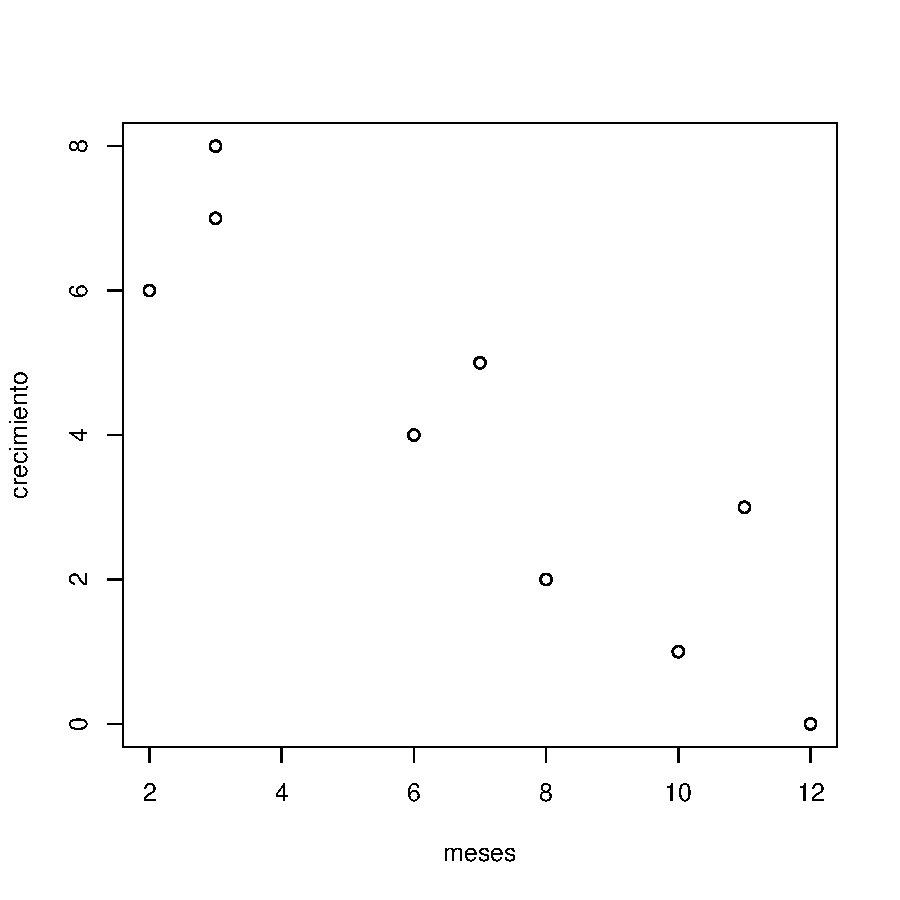
\includegraphics[scale=0.5]{GrapRLS.pdf}}
\end{block}


\end{frame}


\section{El modelo}
\begin{frame}
\frametitle{El modelo de Regresión lineal simple}
\begin{block}{}
\uncover<2->{En realidad, en un análisis más riguroso, el modelo de regresión
lineal es el siguiente:
$$\mu_{Y/x}=\beta_0+\beta_1 x,$$
donde $\mu_{Y/x}$ es el valor esperado  que toma la variable $y$
cuando la variable de control vale $x$, mientras que $\beta_0$
(término independiente) y $\beta_1$ (pendiente) son dos
parámetros a determinar.
}
\end{block}
\begin{block}{}
\uncover<3->{Dada una muestra calcularemos las estimaciones $b_0$ y $b_1$ de
$\beta_0$ y de $\beta_1$ respectivamente. Notemos que para
muestras diferentes, las estimaciones serán diferentes.

Una vez obtenidas las estimaciones podemos calcular la recta de
regresión estimada, que es:\newline
$\hat{y}=b_0+b_1 x.$}
\end{block}

\end{frame}

\section{Mínimos cuadrados}
\begin{frame}
\frametitle{Regresión lineal simple por Mínimos cuadrados}

\begin{block}{}
\begin{itemize}
\item<2->{Existen diversas maneras de calcular las estimaciones de  los
coeficientes de una regresión lineal: Regresión ortogonal, métodos
robustos, regresión mínimo cuadrática o de mínimos cuadrados,...
Nosotros optaremos por el método más habitual que es el de mínimos
cuadrados (m.c.).}
\item<3->{Modelo
$$Y_i=\beta_0+\beta_1 x_i+ E_i,$$
Donde $E_i$ es una nueva variable llamada error o residuo.}
\item<4->{Una vez planteado el modelo  y dada una muestra el modelo se debe
ajustar a los datos de ésta:
$$y_i=\beta_0+\beta_1 x_i+ E_i,\, \mbox{para } i=1,2,\ldots n.$$}
\end{itemize}
\end{block}
\end{frame}

\begin{frame}
\frametitle{Regresión lineal simple por Mínimos cuadrados}

\begin{itemize}
\item<2->{Cuando ajustamos por las estimaciones $b_0$ y $b_1$
obtenemos la recta de regresión ajustada
$$\hat{y}=b_0+b_1 x.$$}

\item<3->{Podemos calcular para cada par de observaciones:

$$y_i= b_0+b_1 x_i+e_i,\qquad \hat{y_i}=b_0+b_1 x_i \mbox{ para } i=1,2,\ldots n.$$}
\item<4->{Entonces el error o residuo de la $i$-ésima observación,
$i=1,2,\ldots,n$, es
$$e_i=y_i-\hat{y}_i.$$}
\end{itemize}
\end{frame}

\subsection{Cálculo de los coeficientes}
\begin{frame}
\frametitle{Regresión lineal simple por Mínimos cuadrados}

\framesubtitle{Cálculo de los coeficientes}

\begin{block}{Cálculo de $b_0$ y $b_1$ por M.C.}
\begin{itemize}
\item<2->{Los valores de $b_0$ y $b_1$ buscados son los que minimizan el
error cuadrático:
$$SSE=\sum_{i=1}^n e_i^2.$$}
\item<3->{Estos valores serán los estimadores de $\beta_0$ y $\beta_1$ por el método de mínimos
cuadrados.}
\end{itemize}
\end{block}
\end{frame}
\begin{frame}
\frametitle{Regresión lineal simple por Mínimos cuadrados}

\framesubtitle{Cáculo de los coeficientes}

\begin{itemize}
\item<2->{En primer lugar tenemos que:
$$SSE=\sum_{i=1}^n e_i^2=\sum_{i=1}^n (y_i-\hat{y}_i)^2=\sum_{i=1}(y_i-b_0-b_1 x_i)^2.$$}
\item<3->{Calculando las derivadas parciales respecto a $b_0$ y a $b_1$, e
igualando a cero:
$$
\begin{array}{ll}\frac{\partial SSE}{\partial b_0}=&-2\sum\limits_{i=1}^n (y_i -b_0-b_1 x_i)=0,\\ & \\
\frac{\partial SSE}{\partial b_1}=&-2\sum\limits_{i=1}^n (y_i -b_0-b_1
x_i) x_i =0.
\end{array}
$$}
\end{itemize}
\end{frame}

\subsection{Ecuaciones normales}

\begin{frame}
\frametitle{Regresión lineal simple por Mínimos cuadrados}
\framesubtitle{Cálculo de los coeficientes. Ecuaciones normales}

\begin{itemize}
\item<2->{Las ecuaciones anteriores reciben el nombre de 
ecuaciones normales:
$$
\left.
\begin{array}{ll}n b_0 + \sum\limits_{i=1}^n x_i b_1&=\sum\limits_{i=1}^n y_i\\ & \\
\sum\limits_{i=1}^n x_i b_0 + \sum\limits_{i=1}^n x_i^2 b_1 &=\sum\limits_{i=1}^n x_i
y_i
\end{array}\right\}
$$}
\item<3->{Las soluciones de estas ecuaciones son:
$$b_1=\frac{n \sum\limits_{i=1}^n x_i y_i-\sum\limits_{i=1}^n x_i\sum\limits_{i=1}^n y_i} {n\sum\limits_{i=1}^n
x_i^2-(\sum\limits_{i=1}^n x_i)^2},\quad b_0=\frac{\sum\limits_{i=1}^n y_i -b_1 \sum\limits_{i=1}^n x_i}{n}.$$}
\end{itemize}
\end{frame}

\begin{frame}
\frametitle{Ejemplo}
\uncover<2->{En el ejemplo anterior, tenemos:
$$b_1=\frac{n \sum\limits_{i=1}^n x_i y_i-\sum\limits_{i=1}^n x_i\sum\limits_{i=1}^n y_i} {n\sum\limits_{i=1}^n
x_i^2-(\sum\limits_{i=1}^n x_i)^2}=\frac{9\cdot 175 -62\cdot 36}{9\cdot 536 - 62^2}=-0.6704,$$
$$b_0=\frac{\sum\limits_{i=1}^n y_i -b_1 \sum\limits_{i=1}^n x_i}{n}=\frac{36-(-0.6704)\cdot 62}{9}=8.6184.$$
}
\end{frame}

\subsection{Momentos de primer y segundo orden.}
\begin{frame}
\frametitle{Regresión lineal simple por Mínimos cuadrados}
\framesubtitle{Cálculo de los coeficientes. Definición de los momentos de primer y segundo orden.}
\begin{itemize}
\item<2->{Definimos las medias y varianzas de las variabes $x$ e $y$ como:
$$
\overline{x}=\frac{\sum\limits_{i=1}^n x_i}{n},\quad \overline{y}=\frac{\sum\limits_{i=1}^n y_i}{n},
$$
$$
s_x^2 =\frac{\sum\limits_{i=1}^n (x_i-\overline{x})^2}{n}=\frac{\sum\limits_{i=1}^n x_i^2}{n}-\overline{x}^2,$$
$$s_y^2 =\frac{\sum\limits_{i=1}^n (y_i-\overline{y})^2}{n}=\frac{\sum\limits_{i=1}^n y_i^2}{n}-\overline{y}^2,
$$}
\end{itemize}
\end{frame}


\begin{frame}
\frametitle{Regresión lineal simple por Mínimos cuadrados}
\framesubtitle{Cálculo de los coeficientes. Definición de los momentos de primer y segundo orden.}
\begin{itemize}
\item<2->{Definimos la covarianza entre las variabes $x$ e $y$ como:
$$
s_{xy}=\frac{\sum\limits_{i=1}^n (x_i-\overline{x}) (y_i-\overline{y})}{n}=\frac{\sum\limits_{i=1}^n x_i y_i}{n}-\overline{x}\overline{y}.
$$}
\end{itemize}
\end{frame}

\begin{frame}
\frametitle{Ejemplo anterior}
\begin{itemize}
\item<2->{Los momentos de primer orden son para el ejemplo anterior:
$$
\overline{x}=\frac{62}{9}=6.89,\quad \overline{y}=\frac{36}{9}=4.
$$}
\item<3->{Los momentos de segundo orden son:
$$
s_x^2=\frac{536}{9}-6.89^2=12.09877, s_y^2 = \frac{204}{9}-4^2=6.67,
$$
$$
s_{xy}=\frac{175}{9}-6.89\cdot 4=-8.111111.
$$}
\end{itemize}
\end{frame}


\subsection{Coeficientes en función de los momentos}
\begin{frame}
\frametitle{Regresión lineal simple por Mínimos cuadrados}
\framesubtitle{Cálculo de los coeficientes en función de los momentos de primer y segundo orden}
\begin{itemize}
\item<2->{Los coeficientes de la recta de regresión son en función de las medias, varianzas y covarianza entre las variables $x$ e $y$:
$$
b_1 =\frac{s_{xy}}{s_x^2},\quad b_0 = \overline{y}-b_1 \overline{x}.
$$}
\item<3->{Ejemplo anterior:
$$
b_1 = \frac{-8.11}{12.09877}=-0.6704,$$
$$
b_0=4-(-0.6704)\cdot 6.89=8.6184.
$$}
\end{itemize}
\end{frame}

\section{Propiedades de los estimadores}
\begin{frame}
\frametitle{Propiedades de los estimadores}

\begin{itemize}
\item<2->{La recta de regresión pasa por el vector de medias
$(\overline{x},\overline{y})$, es decir:
$$b_0+b_1 \overline{x}=\overline{y}$$}

\item<3->{La media de los valores estimados es igual a la media de
los observados
$$\overline{\hat{y}}=\frac{\sum_{i=1}^n\hat{y}_i}
{n}=\overline{y}$$}
\end{itemize}

\end{frame}

\begin{frame}
\frametitle{Ejemplo anterior}
\begin{itemize}
\item<2->{Comprobemos que la recta de regresión pasa por el vector de medias que será $(6.89,4)$:
$$
\begin{array}{l}
\hat{y}=b_0 + b_1 x,\mbox{ si $x=6.89$, queda }\\
8.6184-0.6704\cdot 6.89\approx 4.
\end{array}
$$}
\item<3->{Veamos que la media de los valores estimados es la misma que los valores observados; o sea, $4$. Los valores estimados son:
$$
\begin{array}{l}
0.57347,\ 1.91429,\  3.25510,\  1.24388,\  4.59591,\\
3.92551,\  7.27755,\  6.60714,\  6.60714
\end{array}
$$
Si hallamos la media, vale efectivamente $4$.}
\end{itemize}
\end{frame}

\section{Consideraciones sobre el modelo}
\begin{frame}
\frametitle{Consideraciones sobre el modelo de regresión lineal}

\begin{itemize}
\item<2->{Se  supone que los errores del modelo $E_i$ tienen una
distribución normal de media 0 y desviación típica $\sigma$.}

\item<3->{Los errores  de la estimación por mínimos
cuadrados tienen media $0$.

Efectivamente,
 $$\sum_{i=1}^n e_i=\sum_{i=1}^n
(y_i-\hat{y}_i)=\sum_{i=1}^n (y_i-b_0-b_1 x_i)=0.$$
En conclusión
$$\overline{e}=\frac{\sum_{i=1}^n e_i}{n}=0,$$
y
$$s_e^2=\frac{\sum_{i=1}^{n}
e^2_i}{n}=\frac{SSE}{n}.$$}
\end{itemize}
\end{frame}

\begin{frame}
\frametitle{Ejemplo anterior}
\begin{itemize}
\item<2->{Para comprobar la normalidad se realiza un QQ test. Los errores son los siguientes:
$$
\begin{array}{l}
-0.57347,\  -0.91429,\  -1.25510,\   1.75612,\  -0.59591,
\\  1.07449,\  -1.27755,\ 0.39286,\   1.3928571,
\end{array}
$$
El qq-test de los errores aparece en el gráfico siguiente:
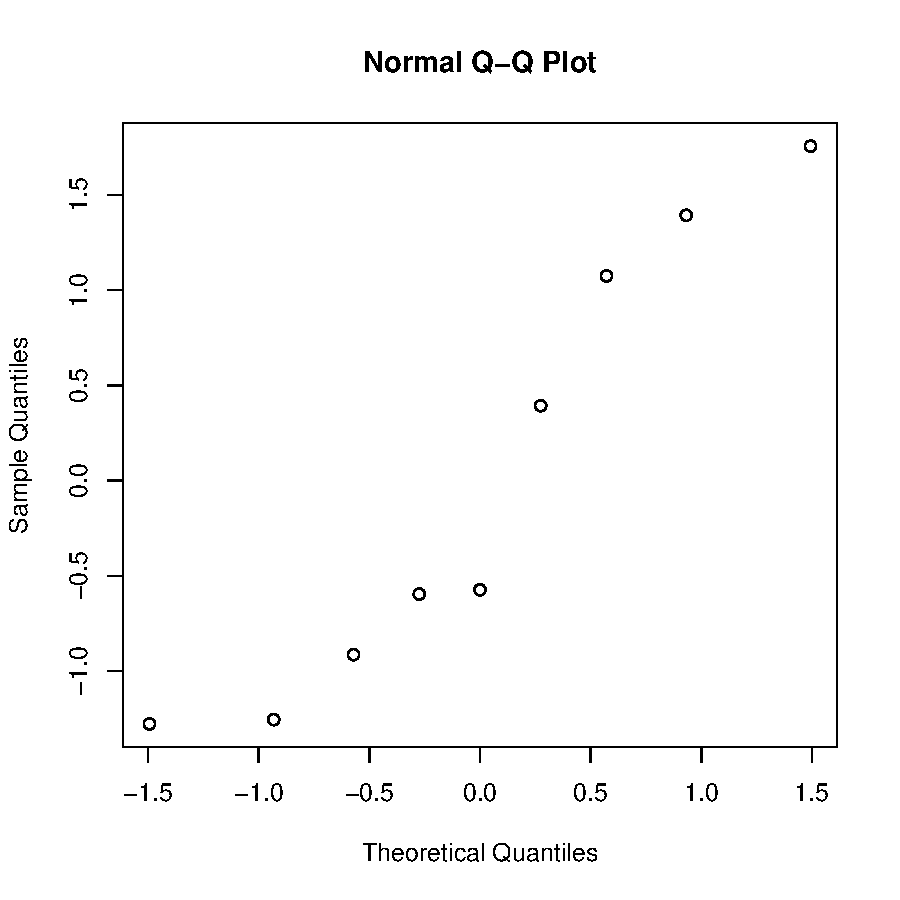
\includegraphics[scale=0.25]{qqtest.pdf}

Para que la normalidad se cumpla los puntos deben estar lo más alineados posible.}
\end{itemize}
\end{frame}
\section{Sumas de cuadrados}
\begin{frame}
\frametitle{Definición de las sumas de cuadrados}

\begin{itemize}
\item<2->{Llamaremos suma de cuadrados de los residuales o del error a
$$SSE=\sum_{i=1}^n(y_i-\hat{y}_i)^2.$$ }
\item<3->{Llamaremos suma de
cuadrados de totales a $$SST =\sum_{i=1}^n(y_i-\overline{y})^2.$$}
\item<4->{Llamaremos suma de cuadrados de la regresión a
$$SSR=\sum_{i=1}^n(\hat{y}_i-\overline{y})^2.$$}
\end{itemize}
\end{frame}

\subsection{Relación entre las sumas de cuadrados}
\begin{frame}
\frametitle{Relación entre las sumas de cuadrados}

\begin{itemize}
\item<2->{En una regresión lineal por el método de mínimos cuadrados se tiene que:
$$SST=SSR+SSE.$$}
\item<3->{La expresión anterior es equivalente a
$$S^2_y=S^2_{\hat{y}}+S^2_e.$$}
\end{itemize}
\end{frame}

\begin{frame}
\frametitle{Ejemplo anterior}
\begin{itemize}
\item<2->{Las sumas de cuadrados son:
$$
\begin{array}{l}
SSE=\sum_{i=1}^n(y_i-\hat{y}_i)^2 =11.06020,\\ SSR=\sum_{i=1}^n(\hat{y}_i-\overline{y})^2 =48.9398,\\
SST =\sum_{i=1}^n(y_i-\overline{y})^2 = 60.
\end{array}
$$
Se puede comprobar que se cumple la igualdad $SST=SSE+SSR$.
}
\end{itemize}
\end{frame}

\section{El coeficiente de determinación $R^2$ y la estimación de la varianza.}
\begin{frame}
\frametitle{El coeficiente de determinación $R^2$ y la estimación de la varianza.}

\begin{itemize}
\item<2->{Se define como $$R^2=\frac{SSR}{SST}.$$}
\item<3->{En el caso de regresión lineal m.c. se cumple que:
$R^2=\frac{S^2_{\hat{y}}}{S^2_y}$, $R^2=1-\frac{SSE}{SST}$, 
$R^2=1-\frac{S^2_e}{S^2_y}$.}
\item<4->{$R^2=r^2_{xy},$ donde $r_{xy}=\frac{s_{xy}}{s_x s_y}$.}
\item<5->{Por lo tanto $R^2$ es la proporción de varianza de la variable $y$
que queda explicada por la regresión lineal.}
\item<6->{Una estimación insesgada de $\sigma^2$ (la varianza del error
$E$) en m.c. es
$$S^2=\frac{SSE}{n-2}.$$}
\end{itemize}
\end{frame}

\begin{frame}
\frametitle{Ejemplo anterior}
\begin{itemize}
\item<2->{El coeficiente $R^2$ valdrá: $R^2 =\frac{48.9398}{60}=0.8157.$ Por tanto, 
se explica el $81.57\%$ de la varianza del crecimiento de la planta.}
\item<3->{Estimación insesgada de la varianza: 
$$S^2 = \frac{SSE}{n-2}=\frac{11.06020}{7}=1.5800.$$}
\end{itemize}
\end{frame}


\section{Intervalos de confianza}
\begin{frame}
\frametitle{Intervalos de confianza}
\begin{itemize}
\item<2->{Suponemos de que los residuos siguen una ley normal.}
\item<3->{Intervalo de confianza al nivel $(1-\alpha)100\%$ para el
parámetro $\beta_1$: ($\mu_{Y/x}=\beta_0+\beta_1 x$)
$$b_1-\frac{t_{n-2,\alpha/2} S}{\sqrt{n S^2_x}}<\beta_1<b_1+\frac{t_{n-2,\alpha/2}S}{\sqrt{
n S^2_x}}$$}
\item<4->{Intervalo de confianza al nivel
$(1-\alpha)100\%$ para el parámetro $\beta_0$: 
$$b_0-\frac{t_{n-2,\alpha/2}S\sqrt{\sum_{i=1}^n x^2_i}}{n
S_{x}}<\beta_0<b_0+\frac{t_{n-2,\alpha/2}S\sqrt{\sum_{i=1}^n
x^2_i}}{n S_{x}}$$}
\end{itemize}
\end{frame}

\begin{frame}
\frametitle{Intervalos de confianza}
\begin{itemize}
\item<2->{Intervalo de confianza al nivel
$(1-\alpha)100\%$ para la respuesta media $\mu_{Y/x_0}$:
$$\hat{y}_0-t_{n-2,\alpha/2}S\sqrt{\frac{1}{n}+\frac{(x_0-\overline{x})^2}{n
S^2_x}}<\mu_{Y/x_0}<$$
$$\hat{y}_0+t_{n-2,\alpha/2}S\sqrt{\frac{1}{n}+\frac{(x_0-\overline{x})^2}{n
S^2_x}}$$}
\item<3->{Intervalo de confianza al nivel
$(1-\alpha)100\%$ para el valor de $y_0$ cuando $x=x_0$:
$$\hat{y}_0-t_{n-2,\alpha/2}S\sqrt{1+\frac{1}{n}+\frac{(x_0-\overline{x})^2}{n
s^2_x}}< y_0 <$$
$$\hat{y}_0+t_{n-2,\alpha/2}S\sqrt{1+\frac{1}{n}+\frac{(x_0-\overline{x})^2}{n
s^2_x}}$$}
\end{itemize}
\end{frame}

\begin{frame}
\frametitle{Ejemplo anterior}
\begin{itemize}
\item<2->{Intervalo de confianza al nivel $95\%$ para la respuesta media $\mu_{Y/x_0}$:
$$
\begin{array}{l}
\hat{y}_0-t_{n-2,\alpha/2}S\sqrt{\frac{1}{n}+\frac{(x_0-\overline{x})^2}{n
s^2_x}}<\mu_{Y/x_0}< \\
\hat{y}_0+t_{n-2,\alpha/2}S\sqrt{\frac{1}{n}+\frac{(x_0-\overline{x})^2}{n
s^2_x}} \\
\hat{y}_0 - t_{7,0.025} \sqrt{\frac{1.58}{9}+\frac{1.58\cdot (x_0 - 6.89)^2}{9\cdot 12.09877}}<\mu_{Y/x_0}< \\
\hat{y}_0 + t_{7,0.025} \sqrt{\frac{1.58}{9} +\frac{1.58\cdot (x_0 - 6.89)^2}{9\cdot 12.09877}} \\
\hat{y}_0 - 2.36\cdot  \sqrt{0.1756 +\frac{(x_0 - 6.89)^2}{68.917}} <\mu_{Y/x_0}< \\
\hat{y}_0 + 2.36\cdot  \sqrt{0.1756 +\frac{(x_0 - 6.89)^2}{68.917}}
\end{array}
$$
Si cogemos $x_0=11$ meses, el intervalo anterior vale: $-0.287<\mu_{Y/x_0}< 2.775.$}
\end{itemize}

\end{frame}

\section{ANOVA}
\begin{frame} 
\frametitle{ANOVA en la recta de regresión lineal}

\uncover<2->{Muy brevemente el Análisis de la Varianza (ANalisys Of VAriance)
consiste en contrastar si la media de una variable en $k$
poblaciones independientes, con distribución normal de igual
varianza, son iguales contra que al menos dos son distintas.
$$\left\{
\begin{array}{rl}
H_0:&\mu_1=\mu_2=\ldots=\mu_k\\
H_1:& \mbox{no todas las medias son iguales}\end{array}\right.$$}


\uncover<3->{En el caso de la regresión lineal, usaremos la técnica anterior para contrastar si las medias de los grupos que conforman las variables son iguales o no (el grupo $k$ está formado por los valores cuya media vale $\mu_{Y/x_k}$). En caso afirmativo, decir que las medias son iguales es equivalente a afirmar que $\beta_1=0$ y, por lo tanto, el modelo de regresión lineal no es bueno.
Por tanto, para que el modelo sea bueno, hemos de rechazar la hipótesis nula en el contraste ANOVA}
\end{frame}

\begin{frame}
\frametitle{ANOVA en la recta de regresión lineal}

\begin{itemize}
\item<2->{Test a realizar:
$$\left\{\begin{array}{rl}H_0:&\beta_1=0\\H_1:&\beta_1\not=0\end{array}\right.$$}

\item<3->{Tabla a calcular:\vskip1cm
\begin{tabular}{|c|c|c|c|c|}\hline
Fuente de & Suma de & g. l. & Cuadrados & \\
variación & cuadrados &  & medios &  $F$\\\hline
Regresión & $SSR$ & $1$ & $SSR$ & $SSR/S^2$ \\
Error & $SSE$ & $n-2$& $S^2=\frac{SSE}{n-2}$ & \\
\hline Total & $SST$ & $n-1$ & & \\\hline\end{tabular}
}
\end{itemize}


\end{frame}

\begin{frame}
\frametitle{ANOVA en la recta de regresión lineal}
\begin{itemize}
\item<2->{Ahora rechazamos la hipótesis nula al nivel de significación $\alpha$ si $f>f_{\alpha,1,n-2}$
donde $f_{\alpha,1,n-2}$ es el valor de una distribución $F$ de
con grados de libertad $1$ y $n-2$.}
\item<3->{Esta prueba, en el caso de regresión lineal simple tiene un efecto
a otra parecida en la que se contrasta con una t de student.}
\end{itemize}

\end{frame}

\begin{frame}
\frametitle{Ejemplo anterior}
\begin{itemize}
\item<2->{Tabla ANOVA:\vskip1cm
\begin{tabular}{|c|c|c|c|c|}\hline
Fuente de & Suma de & g. l. & Cuadrados & \\
variación & cuadrados &  & medios &  $F$\\\hline
Regresión & $48.9398$ & $1$ & $48.9398$ & $30.974$ \\
Error & $11.0602$ & $7$& $S^2=1.5800$ & \\
\hline Total & $60$ & $8$ & & \\\hline\end{tabular}}
\item<3->{Cogemos $\alpha =0.05$. El valor $f_{0.05,1,7}$ vale $5.59$. Como $f=30.974 > 5.59$, rechazamos la hipótesis nula y concluimos que $\beta_1\not=0$. Por tanto, nuestro modelo es adecuado según este análisis.}
\end{itemize}

\end{frame}

\chapter{Regresión lineal múltiple}
%\frame{\partpage}
\section{Introducción}
\begin{frame}
\frametitle{Introducción}
\begin{itemize}
\item<2->{Tenemos $k$ variables independientes $x_1,\ldots, x_k$ y una
variable dependiente $y$.}

\item<3->{Postulamos el modelo de regresión lineal como:
$$\mu_{Y,x_1,\ldots,x_k}= \beta_0+\beta_1 x_1+\ldots\beta_k x_k.$$
Los parámetros $\beta_i$ son desconocidos y se pueden estimar a
partir de una muestra:
$$\{(x_{i1},x_{i2},\ldots,x_{ik},y_i)| i=1,2,\ldots,n\}$$
de la que se exige que $n>k$, es decir el número de observaciones
sea mayor que el número de variables.}
\end{itemize}
\end{frame}

\begin{frame}
\frametitle{Introducción}
\begin{itemize}
\item<2->{El modelo es el siguiente: Consideramos una conjunto de $k$ variables aleatorias $X_{1 },X_{2},\ldots,X_{k}$.
Suponemos que existen variables aleatorias respuestas $Y_1,\ldots,Y_k$ cuya relación con las anteriores es:
$$Y_i=\beta_0+\beta_1 X_{1}+\cdots+\beta_{k} X_k+E_i,$$
donde $E_i$ son variables aleatorias que representan el error aleatorio del modelo asociado a la respuesta $Y_i$.}
\item<3->{El problema es estimar los parámetros $\beta_i$ a
partir de una muestra de datos que representan una muestra aleatoria simple de las variables $X_i$ y de la variable $Y$ de tamaño $n$:
$$\{(x_{i1},x_{i2},\ldots,x_{ik},y_i)| i=1,2,\ldots,n\}.$$
}
\end{itemize}
\end{frame}


\begin{frame}
\frametitle{Introducción}

\begin{itemize}
\item<2->{Llamaremos $y_i$ al valor obtenido de la variable $Y_i$ usando las estimaciones $b_i$ de los parámetros $\beta_i$:
$$y_i=b_0+b_1 x_{i1}+\cdots+b_{k} x_{ik}+e_i\mbox{ para } i=1,2,\ldots,n$$
donde $e_i$ será la estimación de la variable error residual $E_i$ asociado  a la respuesta $Y_i$.}
\item<3->{Llamaremos
$$\hat{y}_i=b_0+b_1 x_{i 1}+\cdots+b_{k} x_{i k}.$$ 
Entonces
$e_i=y_i-\hat{y}_i.$}
\end{itemize}
\end{frame}

\begin{frame}
\frametitle{Introducción}
\begin{itemize}
\item<2->{Definimos los vectores siguientes:
$$
\vect{y}=
\left(
\begin{array}{l}
y_1\\ y_2\\\vdots\\ y_n
\end{array}\right),\  \vect{b}=\left(
\begin{array}{l}
b_0\\ b_1\\\vdots\\b_k
\end{array}\right),\ \vect{\hat{y}}=\left(
\begin{array}{l}
\hat{y}_1\\ \hat{y}_2\\\vdots\\\hat{y}_n
\end{array}\right),\ \vect{e}=\left(
\begin{array}{l}
e_1\\ e_2\\\vdots\\ e_n
\end{array}\right).
$$}
\item<3->{Definimos la matriz siguiente:
$$
\vect{X}=\left(
\begin{array}{lllll}
1&x_{11}&x_{12}&\ldots&x_{1k}\\
1&x_{21}&x_{22}&\ldots&x_{2k}\\
\vdots&\vdots&\vdots&\vdots&\vdots\\
1&x_{n1}&x_{n2}&\ldots&x_{nk}
\end{array}
\right)$$}
\end{itemize}
\end{frame}
\begin{frame}
\frametitle{Introducción}
\begin{itemize}
\item<2->{Podemos escribir el modelo de regresión múltiple matricialmente como:
$$
\begin{array}{rl}
\vect{y}= & \vect{X}\vect{b}+\vect{e},\\
\vect{\hat{y}} = & \vect{X}\vect{b}, \\
\vect{e} = & \vect{y}-\vect{\hat{y}}.
\end{array}$$}
\end{itemize}
\end{frame}

\section{Mínimos cuadrados}
\begin{frame}
\frametitle{Cálculo de los coeficientes $b_i$ usando el método de mínimos cuadrados}
\begin{itemize}
\item<2->{Definimos el error cuadrático $SSE$ como:
$$
\begin{array}{rl}
SSE=&\sum\limits_{i=1}^n
e^2_i=\sum\limits_{i=1}^n (y_i-\hat{y}_i)^2 \\ 
=&\sum\limits_{i=1}^n (y_i-b_0-b_1 x_{i 1}-\cdots -b_{k} x_{ik})^2.
\end{array}$$}
\item<3->{Los estimadores por el método de mínimos cuadrados serán los
valores $b_0,b_1,\ldots, b_k$ que minimicen $SSE$.
}
\item<4->{Para resolver este problema calculamos las derivadas parciales de
SSE respecto a cada $b_i$ para $i=1,2,\ldots,n$ y se obtiene el
un sistema de ecuaciones que recibe el nombre de ecuaciones normales.
}
\end{itemize}
\end{frame}

\begin{frame}
\frametitle{Cálculo de los coeficientes $b_i$ usando el método de mínimos cuadrados}
\uncover<2->{$$
\left.
\begin{array}{rl}
n b_0 +b_1 \sum\limits_{i=1}^n x_{i 1}+\ldots + b_k \sum\limits_{i=1}^n x_{i
k} &=  \sum\limits_{i=1}^n y_i\\ & \\
b_0 \sum\limits_{i=1}^n x_{i 1}+b_1 \sum\limits_{i=1}^n x^2_{i 1}+
b_2\sum\limits_{i=1}^n x_{i 1} x_{i 2}+ \ldots +& \\ &\\ b_k \sum\limits_{i=1}^n x_{i
1}x_{ik} & =  \sum\limits_{i=1}^n x_{i 1}y_i\\
\ldots & \ldots \\
b_0 \sum\limits_{i=1}^n x_{i k}+b_1 \sum\limits_{i=1}^n x_{i k}x_{i 1}+
b_2\sum\limits_{i=1}^n x_{i k} x_{i 2}+\ldots + & \\ &\\  b_k \sum\limits_{i=1}^n x^2_{i
k} & = \sum\limits_{i=1}^n x_{i k}y_i\\\end{array}\right\}
$$}
\end{frame}

\begin{frame}
\frametitle{Cálculo de los coeficientes $b_i$ usando el método de mínimos cuadrados}
\begin{itemize}
\item<2->{El sistema anterior se puede expresar en forma matricial de la forma siguiente: 
$$
\left(\vect{X}^\top\vect{X}\right)\cdot \vect{b}=\vect{X}^\top\cdot \vect{y}.
$$}
\item<3->{La solución buscada del sistema anterior será:
$$
\vect{b}=\left(\vect{X}^\top\vect{X}\right)^{-1}\cdot \left(\vect{X}^\top \vect{y}\right).
$$}
\end{itemize}

\end{frame}
\begin{frame}
\frametitle{Ejemplo}
\begin{itemize}
\item<2->{Se postula que la estatura de un niño recién nacido ($y$)  tiene
una relación con su edad en días $x_1$, su estatura al nacer en
cm. ($x_2$), su peso en Kg. al nacer ($x_3$) y el aumento en tanto por ciento de su peso actual con respecto a su peso al nacer ($x_4$). Se pudo obtener una pequeña muestra con $n=9$
niños cuyos resultados fueron:}
\item<3->{\begin{center}\begin{tabular}{|c|c|c|c|c|}\hline
$y$ & $x_1$ & $x_2$ & $x_3$ & $x_4$\\\hline
57.5&78&48.2&2.75&29.5\\ 52.8&69&45.5&2.15&26.3\\
61.3&77&46.3&4.41&32.2\\ 67&88&49&5.52&36.5\\ 53.5&67&43&3.21&27.2\\
62.7&80&48&4.32&27.7\\ 56.2&74&48&2.31&28.3\\ 68.5&94&53&4.3&30.3\\
69.2&102&58&3.71&28.7\\\hline\end{tabular}\end{center}}
\end{itemize}
\end{frame}
\begin{frame}
\frametitle{Ejemplo}
\begin{itemize}
\item<2->{La matriz $\vect{X}$ es:
$$
\vect{X}=\left(
\begin{array}{lllll}
1&78&48.2&2.75&29.5\\
1&69&45.5&2.15&26.3\\
1&77&46.3&4.41&32.2\\
1&88&49&5.52&36.5\\
1&67&43&3.21&27.2\\
1&80&48&4.32&27.7\\
1&74&48&2.31&28.3\\
1&94&53&4.3&30.3\\
1&102&58&3.71&28.7
\end{array}
\right)
$$}
\end{itemize}
\end{frame}
\begin{frame}
\frametitle{Ejemplo}
\begin{itemize}
\item<2->{El vector $\vect{y}$ es:
$$
\vect{y}=\left(
\begin{array}{l}
57.5\\ 52.8\\ 61.3\\ 67\\ 53.5\\ 62.7\\ 56.2\\ 68.5\\ 69.2
\end{array}
\right)
$$}
\end{itemize}
\end{frame}
\begin{frame}
\frametitle{Ejemplo}
\begin{itemize}
\item<2->{El producto $\vect{X}^\top\vect{X}$ es el siguiente:
$$
\left(
\begin{array}{lllll}
9& 729&   439&  32.68 & 266.7 \\
729& 60123& 35947.2& 2702.41& 21715.3\\
439& 35947.2& 21568.18& 1604.388& 13026.01\\
66.07 & 6108.19 & 3541.008& 128.66&  1948.561\\
266.7& 21715.3&13026.01& 990.27&  7980.83
\end{array}
\right)
$$}
\item<3->{El producto $\vect{X}^\top\vect{y}$ es el siguiente:
$$
\vect{X}^\top\vect{y} = \left(
\begin{array}{l}
548.7\\ 45001\\ 26946.89\\ 2035.52\\ 16348.29
\end{array}
\right)
$$}
\end{itemize}
\end{frame}
\begin{frame}
\frametitle{Ejemplo}
\begin{itemize}
\item<2->{Resolviendo el sistema $(\vect{X}^\top\vect{X})\cdot \vect{b}=\vect{X}^\top \vect{y}$ obtenemos como solución:
$$
\vect{b}=\left(
\begin{array}{l}
7.1475 \\ 0.1001 \\ 0.7264 \\ 3.0758\\ -0.03
\end{array}
\right)
$$}
\item<3->{La recta de regresión estimada es :
$$\hat{y}=7.1475 +   0.1001 x_1+0.7264 x_2 +3.0758 x_3-0.03 x_4.$$}
\end{itemize}
\end{frame}
\section{Propiedades}
\begin{frame}
\frametitle{Propiedades de la recta de regresión}
\begin{itemize}
\item<2->{La recta de regresión ajustada pasa por el vector de
medias. O sea, si llamamos $\overline{x}_j=\frac{\sum\limits_{i=1}^n x_{ij}}{n},$ para $i=1,\ldots,k$, $\overline{y}=\frac{\sum\limits_{i=1}^n y_i}{n}$, se verifica que:
$$
\overline{y}=b_0 + b_1\overline{x}_1+\cdots +b_k \overline{x}_k.
$$}
\item<3->{La suma de los errores $e_i$ es $0$: $\sum\limits_{i=1}^n
e_i=0$ y por lo tanto su media también: $\overline{e}=0$.}
\item<4->{La media de los valores estimados coincide con la media de los valores de la muestra: $\overline{\hat{y}}=\overline{y}$.}
\end{itemize}
\end{frame}
\begin{frame}
\frametitle{Ejemplo}
\begin{itemize}
\item<2->{Veamos que la recta de regresión pasa por el vector de medias. Éste vale:
$$
\overline{x}_0 = 1,\ \overline{x}_1=81,\ \overline{x}_2 =48.778,\ \overline{x}_3=3.631,\ \overline{x}_4 = 29.633.
$$
La media del vector $\vect{y}$ vale: $\overline{y}=60.967$.

Se cumple:
$$
\begin{array}{rl}
60.967 \approx  & 7.1475 +  0.1001\cdot 81 +0.7264\cdot 48.778 \\ & +3.0758\cdot 3.6311-0.03\cdot 29.633.
\end{array}
$$
}

\end{itemize}
\end{frame}

\begin{frame}
\frametitle{Ejemplo}
\begin{itemize}
\item<2->{Veamos que la media de los errores es nula.
Los valores de los vectores $\vect{\hat{y}}$ y $\vect{e}$ son:
$$
\vect{\hat{y}}=\vect{X}\cdot b =  \left(\begin{array}{l}
 57.541 \\  52.929 \\  61.085 \\ 67.432 \\ 54.146 \\  62.479 \\ 55.678  \\   67.372 \\ 70.039      \end{array}\right),\ \vect{e}=\vect{y}-\vect{\hat{y}}=\left(\begin{array}{l}
    -0.0405\\ -0.1290\\ 0.2150\\ -0.4324 \\ -0.6461 \\ 0.2214 \\ 0.5225 \\ 
 1.1277\\ -0.8385 \end{array}\right)
$$}
\item<3->{Puede comprobarse que la media del vector $\vect{e}$ es $0$ y que $\overline{\hat{y}}=\overline{y}=60.967$.}
\end{itemize}
\end{frame}


\section{Sumas de cuadrados}
\begin{frame}
\frametitle{Sumas de cuadrados en la regresión}
\begin{itemize}
\item<2->{Llamaremos suma de cuadrados de los residuales o del error a
$$SSE=\sum_{i=1}^n (y_i-\hat{y}_i)^2.$$}
\item<3->{Llamaremos suma de cuadrados de totales a 
$$SST=\sum_{i=1}^n (y_i-\overline{y})^2.$$}
\item<4->{Llamaremos suma de
cuadrados de la regresión a
$$SSR=\sum_{i=1}^n(\hat{y}_i-\overline{y})^2.$$}
\item<5->{Se verifica:
$$SST=SSR+SSE,$$
o equivalentemente:
$$S^2_y=S^2_{\hat{y}}+S^2_e.$$}
\end{itemize}
\end{frame}

\begin{frame}
\frametitle{Ejemplo}
\begin{itemize}
\item<2->{La suma de cuadrados del error vale en el ejemplo anterior:
$$
SSE =(57.5-57.5405)^2+\cdots +(69.2-70.0385)^2 = 2.9656.
$$}
\item<3->{La suma de cuadrados totales vale:
$$
SST=(57.5-60.967)^2+\cdots +(69.2-60.967)^2 = 321.24.
$$}
\item<4->{La suma de cuadrados de la regresión es:
$$
\begin{array}{rl}
SSR= & (57.5405-60.967)^2 +\cdots +(70.0385-60.967)^2 \\ 
= & 318.274.
\end{array}
$$}
\item<5->{Puede observarse que se cumple: 
$$
SST=SSE+SSR,\quad 321.24 = 2.9656 + 318.274.
$$}
\end{itemize}
\end{frame}


\section{Coeficiente de determinación}
\begin{frame}
\frametitle{Definición del coeficiente de determinación}
\begin{itemize}
\item<2->{Definimos el coeficiente de determinación como
$$R^2=\frac{SSR}{SST}=1-\frac{SSE}{SST},$$
o también
$$R^2=\frac{S^2_{\hat{y} }}{S^2_y}=1-\frac{S^2_e}{S^2_y}.$$
$R^2$  se interpreta como la proporción de varianza de la variable
$y$ que es explicada por el modelo de regresión múltiple.
}
\item<3->{Definimos el coeficiente de determinación ajustado como:
$$R^2a=R^2-\frac{k(1-R^2)}{n-k-1}.$$}
\item<4->{Definimos el coeficiente de correlación múltiple $r$ de la variable $y$ respecto de las variables $x_1,\ldots, x_k$ como $r=\sqrt{R^2}$.}
\end{itemize}
\end{frame}

\begin{frame}
\frametitle{Ejemplo}
\begin{itemize}
\item<2->{El coeficiente de determinación vale en nuestro ejemplo:
$$
R^2 = \frac{318.274}{321.24} \approx 0.9908.
$$}
\item<3->{El coeficiente de determinación ajustado vale:
$$
R^2a = 0.9908 -\frac{4\cdot (1-0.9908)}{9-4-1} = 0.9815.
$$}
\item<4->{El coeficiente de correlación múltiple $r$ de la variable $y$ respecto de las variables $x_1,\  x_2,\ x_3,\ x_4$ vale: $r=\sqrt{0.9908}=0.9954.$}
\end{itemize}
\end{frame}
\section{Consideraciones sobre el modelo}
\begin{frame}
\frametitle{Consideraciones sobre el modelos de regresión múltiple}
\begin{itemize}
\item<2->{Suponemos que las variables aleatorias error $E_i$ son
independientes e idénticamente distribuidas  según una normal de
media $0$ y varianza $\sigma^2$.}
\item<3->{Bajo el supuesto anterior,
los estimadores $b_0,\ldots, b_k$ de
$\beta_0,\ldots,\beta_k$ son insesgados. O sea, $E(b_i)=\beta_i,\ i=0,\ldots, k$.}
\item<4->{La matriz $(X^\top X)^{-1} \sigma^2$ es la matriz de covarianzas de
$\beta_0,\ldots,\beta_k$.}
\item<5->{Un estimador insesgado de
$\sigma^2$ es $$S^2=\frac{SSE}{n-k-1}.$$}
\end{itemize}
\end{frame}
\begin{frame}
\frametitle{Ejemplo}
\begin{itemize}
\item<2->{Una estimación de la varianza $\sigma^2$ será:
$$
S^2 = \frac{2.9656}{9-4-1}=0.7414.
$$}
\item<3->{Una estimación de la matriz de covarianzas de $\beta_0,\ldots, \beta_4$: $(X^\top X)^{-1} S^2 = $
$$
\left(
\begin{array}{lllll}
270.919 & 5.325 &  -12.521 &  -13.743 &  -1.4 \\
5.325 & 0.115 & -0.266 & -0.326 & -0.0176 \\
-12.521 &  -0.266 & 0.618 &  0.742 & 0.0416 \\
-13.743 &  -0.326 &  0.742 &  1.122 &  -0.00598 \\
-1.4 & -0.0176 & 0.0416 &  -0.00598 &  0.0277
\end{array}
\right)
$$}
\end{itemize}
\end{frame}
\section{ANOVA}
\begin{frame}
\frametitle{ANOVA en regresión lineal múltiple}
\begin{itemize}
\item<2->{El contraste ANOVA en la regresión lineal múltiple nos permite contrastar la adecuación del modelo. Se trata de contrastar: 
$$\left\{\begin{array}{rl} H_0:& \beta_1=\beta_2=\cdots=\beta_k=0 \\
H_1: & \mbox{hay alguna }\beta_i\not= 0 \end{array}\right.$$
}
\item<3->{Si aceptamos $H_0$ estamos diciendo que la estimación dada por la
regresión es constante. Por tanto el modelo no sería adecuado.}
\item<4->{En la tabla siguiente aparece los pasos necesarios para realizar el contraste. Como puede observarse, se usa como estadístico de contraste el cociente $\frac{MSR}{MSE}$ que, suponiendo normalidad, sigue una distribución $F$ de Snédecor de $k,n-k-1$ grados de libertat:
}
\end{itemize}
\end{frame}
\begin{frame}
\frametitle{ANOVA en regresión lineal múltiple}
\uncover<2->{\begin{tabular}{|c|c|c|c|c|}\hline
F.V. & S.C. & g.l. & C.M. & $f$\\\hline
Regresión & $SSR$ & $k$ & $MSR=\frac{SSR}{k}$ & $f=\frac{MSR}{MSE}$ \\ &&&&\\
Error & $SSE$ & $n-k-1$& $MSE=\frac{SSE}{n-k-1}$ & \\
\hline Total & $SST$ & $n-1$ & & \\\hline\end{tabular} 
\begin{description}
\item F.V.: Fuente de variación.
\item S.C.: Suma de cuadrados.
\item g.l.: grados de libertad.
\item C.M.: Cuadrados medios.
\end{description}
}
\uncover<3->{Rechazaremos la hipótesis nula  $H_0: \beta_1=\ldots=\beta_k =0$ al
nivel de significación $\alpha$ si $f>f_{\alpha,k,n-k-1}$
donde $f_{\alpha,k,n-k-1}$ es el valor crítico de una distribución
$F$ de con grados de libertad $k$ y $n-k-1$.}
\end{frame}
\begin{frame}
\frametitle{Ejemplo}
\begin{itemize}
\item<2->{La tabla ANOVA es en nuestro ejemplo:
\begin{center}\begin{tabular}{|c|c|c|c|c|}\hline
F.V. & S.C. & g.l. & C.M. & $f$\\\hline
Regresión & $318.274$ & $4$ & $MSR=79.569$ & $f=107.323$ \\ &&&&\\
Error & $2.9656$ & $4$& $MSE=0.7414$ & \\
\hline Total & $321.24$ & $8$ & & \\\hline\end{tabular}\end{center}}
\item<3->{Cogiendo $\alpha =0.05$, el valor crítico $f_{0.05,4,4}$ vale $6.388.$ Como $f=107.323 > f_{0.05,4,4}=6.388$, rechazamos la hipótesis nula y concluimos que el modelo es adecuado según este análisis.}
\end{itemize}
\end{frame}
\begin{frame}
\frametitle{ANOVA en regresión lineal múltiple}
\begin{itemize}
\item<2->{El modelo de regresión lineal con este conjunto de $x$
puede no ser el único que se puede utilizar. Es posible que con
algunas transformaciones de las $x$ mejore el valor de $f$.}
\item<3->{El modelo podría ser más eficaz si se incluyen otras variables o
podría continuar siendo casi igual de eficaz si se eliminan
algunas (principio de parsimonia).}
\end{itemize}
\end{frame}
\section{Intervalos de confianza}
\begin{frame}
\frametitle{Intervalos de confianza}
\begin{itemize}
\item<2->{Un intervalo de confianza al nivel $(1-\alpha) 100\%$ para la
respuesta media $\mu_{Y/x_{10},x_{20},\ldots,x_{k0}}$ es
$$\hat{y}_0 -t_{\alpha/2,n-k-1} S\sqrt{x^\top_0 (X^\top X)^{-1}
x_0}<$$
$$\mu_{Y/x_{10},x_{20},\ldots,x_{k0}} <\hat{y}_0
+t_{\alpha/2,n-k-1} S\sqrt{x^\top_0 (X^\top X)^{-1} x_0}$$
donde $t_{\alpha/2,n-k-1}$ es el valor crítico de una $t$ de
student con $n-k-1$ grados de libertad, 
$x_0=\left(1,
x_{10},x_{20},\ldots ,x_{k0}\right)^\top$ y $\hat{y}_0 = b_0 + b_1 x_{10} + \cdots +b_k x_{k0}.$}
\item<3->{La cantidad $S\sqrt{x^\top_0 (X^\top X)^{-1} x_0}$ recibe el nombre de
error estándar de predicción.
}
\end{itemize}
\end{frame}
\begin{frame}
\frametitle{Ejemplo}
\begin{itemize}
\item<2->{Para $\alpha =0.05$, hallemos un intervalo de confianza para la respuesta media $\mu_{Y/x_{10},x_{20},x_{30},x_{40}}$, para $x_{10} =69,\ x_{20} = 45.5,\ x_{30} = 2.15,\  x_{40} = 26.3$.}
\item<3->{El valor crítico $t_{0.025,4}$ vale $2.776$. El valor $\hat{y}_0$ valdrá:
$$
\begin{array}{rl}
\hat{y}_0 = & b_0 +\sum_{i=1}^4 b_i x_{i0} \\
= & 7.1475+0.1001\cdot 69 +0.7264\cdot 45.5+3.0758\cdot 2.15 \\ & -0.03\cdot 26.3 
=  52.929.
\end{array}
$$}
\item<4->{
El valor de $x^\top_0 (X^\top X)^{-1} x_0$ es:
$$
(1,69,45.5,2.15,26.3)\cdot (X^\top X)^{-1}\cdot \left(\begin{array}{l}
1\\ 69 \\ 45.5\\ 2.15 \\ 26.3\end{array}\right) = 0.3615.
$$}
\end{itemize}
\end{frame}
\begin{frame}
\frametitle{Ejemplo}
\uncover<2->{El intervalo de confianza será:
$$
\begin{array}{l}
52.929-2.776\sqrt{0.7414\cdot 0.3615}<\mu_{Y/x_{10},x_{20},x_{30},x_{40}} \\
< 52.929+2.776\cdot\sqrt{0.7414\cdot 0.3615} = \\
51.492 <\mu_{Y/x_{10},x_{20},x_{30},x_{40}} < 54.366.
\end{array}
$$
}
\end{frame}
\begin{frame}
\frametitle{Intervalos de confianza}
\begin{itemize}
\item<2->{Un intervalo de confianza al nivel $(1-\alpha) 100\%$ para
una predicción individual $y_0$ para los valores de la variables
dependientes $x_{10},x_{20},\ldots,x_{k0}$ es
$$ \hat{y}_0 -t_{\alpha/2,n-k-1} S\sqrt{1+x^\top_0 (X^\top X)^{-1} x_0}<y_0
<$$
$$\hat{y}_0 +t_{\alpha/2,n-k-1} S\sqrt{1+x^\top_0 (X^\top X)^{-1}
x_0},$$
donde $t_{\alpha/2,n-k-1}$ es el valor crítico de una $t$ de
student con $n-k-1$ grados de libertad, y
$x_0=\left(1,x_{10},x_{20},\ldots,x_{k0}\right)^\top.$}
\end{itemize}
\end{frame}
\begin{frame}
\frametitle{Intervalos de confianza}
\begin{itemize}
\item<2->{Un intervalo de confianza al nivel $(1-\alpha) 100\%$ para el parámetro $\beta_k$ es:
$$
b_k -t_{\alpha/2,n-k-1} s_{\beta_k} < \beta_k < b_k + t_{\alpha/2,n-k-1} s_{\beta_k},
$$
donde $s_{\beta_k}$ es la raiz cuadrada del elemento $k$-ésimo de la diagonal de la matriz $(X^\top X)^{-1} S^2$:
$s_{\beta_k} =\sqrt{\left((X^\top X)^{-1} S^2 \right)_{kk}}$.}
\end{itemize}
\end{frame}
\begin{frame}
\frametitle{Ejemplo}
\begin{itemize}
\item<2->{Para $\alpha =0.05$, hallemos un intervalo de confianza para el parámetro $\beta_2$.}
\item<3->{El valor crítico $t_{0.025,4}$ vale $2.776$. Los valores de la diagonal de la matriz $(X^\top X)^{-1} S^2$ son:
$$
270.919,\quad 0.1154,\quad 0.6176,\quad 1.1219,\quad 0.02775.
$$
El valor que nos interesa es para el parámetro $\beta_2$: $0.726$.}
\item<4->{El intervalo será:
$$
\begin{array}{rl}
0.726-2.776\cdot \sqrt{0.6176}<  & \beta_2  \\ <  0.726+2.776\cdot \sqrt{0.6176} , &\\
-1.4556 < & \beta_2 < 2.908.
\end{array}
$$}
\end{itemize}
\end{frame}

\section{Selección del modelo. Colinealidad}
\begin{frame}
\frametitle{El problema de la selección del modelo. Colinealidad}
\begin{itemize}
\item<2->{Dado un problema regresión lineal múltiple podemos  ajustar
todos los submodelos lineales posibles
$$
\begin{array}{rl}
Y=&\beta_0+ \beta_1 x_1,\\
Y=&\beta_0+ \beta_1 x_1+\beta_2 x_2,\\
&\ldots\\
Y=&\beta_0+ \beta_1 x_1+\cdots +\beta_k x_k,
\end{array}
$$
ya que es posible que entre variables $x_i$ exista una fuerte
relación lineal y entonces \emph{sobren del modelo}. Este problema
recibe el nombre de colinealidad.}
\item<3->{Existen también otro tipo de problemas que se pueden resolver usando la técnica de la regresión lineal múltiple. Véase como ejemplo el problema de la regresión polinomial:
$$Y=\beta_0+ \beta_1 x+\beta_2 x^2+\cdots +\beta_k x^k.$$
}
\end{itemize}
\end{frame}
\begin{frame}
\frametitle{El problema de la selección del modelo. Colinealidad}
\uncover<2->{Una solución para ver qué modelo lineal es el más simple y
adecuado es  recurrir a los llamados métodos secuenciales de
selección del modelo lineal, como son los siguientes:
\begin{itemize}
\item Regresión paso paso (Stepwise). 
\item Selección hacia adelante(Forward).
\item Selección hacia atrás (Backward).
\end{itemize}
}
\end{frame}


\part{Métodos de reducción  o selección de los factores}
 \include{09Acp}
 \include{10EscaladoMultidimensional}
 


%\part{Análisis de correspondencias}
%\frame{\partpage}


\chapter{Analisis de Correspondencias}
\section{Introducción}



\begin{frame}
\frametitle{Introducción}
\begin{itemize}
\item<2->{El análisis de correspondencias es una técnica descriptiva para representar y estudiar tablas de contingencia de variables cualitativas. Es decir, vamos a estudiar las frecuencias de aparición de dos o más variables cualitativas en un conjunto de elementos.}
\item<3->{Dicho análisis constituye la aplicación de técnicas de componentes principales y escalado multidimensional vistas anteriormente para variables cualitativas.}
\item<4->{Nuestra información de partida es una matriz $\vect{X}$ de dimensiones $I\times J$ donde cada valor de la matriz representa la frecuencia absoluta observada de dos variables cualitativas en $n$ elementos.}
\item<5->{Suponemos que la primera variable puede tomar $I$ valores diferentes y que la segunda variable, $J$. Entonces, $x_{ij}$ sería el número de elementos de entre los $n$ que toma el valor $i$-ésimo para la primera variable y toma el valor $j$-ésimo para la segunda.}
\end{itemize}
\end{frame}

\begin{frame}
\frametitle{Ejemplo}
\begin{itemize}
\item<2->{Consideremos el siguiente experimento: tenemos $61$ ratas adultas y $61$ crías de rata. Cada rata puede tener un genotipo diferente de entre cuatro: A, B, I y J. Ponemos cada cría aleatoriamente junto con una rata adulta para que crezca. Al cabo de 28 días, anotamos el porcentaje de peso adquirido por la cría de rata. Anotamos los resultados obtenidos en la tabla siguiente:
{\tiny\begin{table}[ht]
\begin{center}
\begin{tabular}{rrrrrrrr}
  \hline
 & 1 & 2 & 3 & 4 & 5 & 6 & 7 \\
\hline
A A&   0 &   0 &   0 &   0 &   1 &   3 &   1 \\
A B&   0 &   1 &   0 &   1 &   1 &   0 &   0 \\
A I&   0 &   0 &   1 &   2 &   0 &   1 &   0 \\
A J&   1 &   1 &   1 &   1 &   1 &   0 &   0 \\
B A&   0 &   0 &   2 &   1 &   1 &   0 &   0 \\
B B&   0 &   0 &   1 &   0 &   0 &   4 &   0 \\
B I&   0 &   0 &   1 &   1 &   2 &   0 &   0 \\
B J&   1 &   0 &   0 &   1 &   0 &   0 &   0 \\
I A&   2 &   0 &   0 &   0 &   0 &   0 &   1 \\
I B&   0 &   0 &   0 &   0 &   1 &   0 &   2 \\
I I&   1 &   1 &   0 &   2 &   0 &   1 &   0 \\
I J&   0 &   1 &   1 &   1 &   0 &   0 &   0 \\
J A&   0 &   0 &   1 &   1 &   2 &   0 &   0 \\
J B&   0 &   0 &   0 &   2 &   1 &   0 &   0 \\
J I&   0 &   1 &   0 &   0 &   1 &   1 &   0 \\
J J&   0 &   2 &   0 &   3 &   0 &   0 &   0 \\
   \hline
\end{tabular}
\end{center}
\end{table}
}}
\end{itemize}
\end{frame}
\begin{frame}
\frametitle{Ejemplo}
\begin{itemize}
\item<2->{La primera fila nos indica el porcentaje de peso adquirido por la cría de rata (1 indica que ha adquirido poco peso y 7 que ha adquirido mucho peso) y la primera columna nos indica el cruce que hemos hecho (por ejemplo B A indica que hemos puesto una cría de rata de genotipo B con una rata adulta de genotipo A).}
\item<3->{La tabla nos da el número de crías de rata que han aumentado un determinado porcentaje de peso en 28 días usando un cruce determinado.}
\end{itemize}
\end{frame}

\section{Búsqueda de la mejor proyección}
\begin{frame}
\frametitle{Búsqueda de la mejor proyección}
\begin{itemize}
\item<2->{Llamaremos $\vect{F}=(f_{ij})_{i=1,\ldots,I,j=1,\ldots,J}$ a la matriz de frecuencias relativas de la tabla de contingencia. Esto es, dividimos cada elemento de la matriz $\vect{X}$ por el número total de elementos~$n$: $f_{ij}=\frac{x_{ij}}{n}$.}
\item<3->{Los elementos de la matriz anterior verifican: $\sum\limits_{i=1}^I\sum\limits_{j=1}^J f_{ij}=1.$}
\item<4->{Cualquier estudio aplicado a dicha matriz debe ser equivalente al estudio aplicado a su traspuesta ya que elegir la variable que va por filas o por columnas es una elección arbitraria y no debe influir en el análisis.}
\end{itemize}
\end{frame}
\begin{frame}
\frametitle{Ejemplo anterior}
\begin{itemize}
\item<2->{En el ejemplo anterior la matriz $\vect{F}$ será:
{\tiny\begin{table}[ht]
\begin{center}
\begin{tabular}{rrrrrrrr}
  \hline
 & 1 & 2 & 3 & 4 & 5 & 6 & 7 \\
\hline
A A&   0/61 &   0/61  &   0/61  &   0/61  &   1/61  &   3/61  &   1/61  \\
A B&   0/61  &   1/61  &   0/61  &   1/61  &   1/61  &   0/61  &   0/61  \\
A I&   0/61  &   0/61  &   1/61  &   2/61  &   0/61  &   1/61  &   0/61  \\
A J&   1/61  &   1/61  &   1/61  &   1/61  &   1/61  &   0/61  &   0/61  \\
B A&   0/61  &   0/61  &   2/61  &   1/61  &   1/61  &   0/61  &   0/61  \\
B B&   0/61  &   0/61  &   1/61  &   0/61  &   0/61  &   4/61  &   0/61  \\
B I&   0/61  &   0/61  &   1/61  &   1/61  &   2/61  &   0/61  &   0/61  \\
B J&   1/61  &   0/61  &   0/61  &   1/61  &   0/61  &   0/61  &   0/61  \\
I A&   2/61  &   0/61  &   0/61  &   0/61  &   0/61  &   0/61  &   1/61  \\
I B&   0/61  &   0/61  &   0/61  &   0/61  &   1/61  &   0/61  &   2/61  \\
I I&   1/61  &   1/61  &   0/61  &   2/61  &   0/61  &   1/61  &   0/61  \\
I J&   0/61  &   1/61  &   1/61  &   1/61  &   0/61  &   0/61  &   0/61  \\
J A&   0/61  &   0/61  &   1/61  &   1/61  &   2/61  &   0/61  &   0/61  \\
J B&   0/61  &   0/61  &   0/61  &   2/61  &   1/61  &   0/61  &   0/61  \\
J I&   0/61  &   1/61  &   0/61  &   0/61  &   1/61  &   1/61  &   0/61  \\
J J&   0/61  &   2/61  &   0/61  &   3/61  &   0/61  &   0/61  &   0/61  \\
   \hline
\end{tabular}
\end{center}
\end{table}
}
}
\end{itemize}
\end{frame}

\begin{frame}
\frametitle{Ejemplo anterior}
\begin{itemize}
\item<2->{O, si se quiere:
{\tiny\begin{table}[ht]
\begin{center}
\begin{tabular}{rrrrrrrr}
  \hline
 & 1 & 2 & 3 & 4 & 5 & 6 & 7 \\
  \hline
A A & 0.00 & 0.00 & 0.00 & 0.00 & 0.02 & 0.05 & 0.02 \\
  A B & 0.00 & 0.02 & 0.00 & 0.02 & 0.02 & 0.00 & 0.00 \\
  A I & 0.00 & 0.00 & 0.02 & 0.03 & 0.00 & 0.02 & 0.00 \\
  A J & 0.02 & 0.02 & 0.02 & 0.02 & 0.02 & 0.00 & 0.00 \\
  B A & 0.00 & 0.00 & 0.03 & 0.02 & 0.02 & 0.00 & 0.00 \\
  B B & 0.00 & 0.00 & 0.02 & 0.00 & 0.00 & 0.07 & 0.00 \\
  B I & 0.00 & 0.00 & 0.02 & 0.02 & 0.03 & 0.00 & 0.00 \\
  B J & 0.02 & 0.00 & 0.00 & 0.02 & 0.00 & 0.00 & 0.00 \\
  I A & 0.03 & 0.00 & 0.00 & 0.00 & 0.00 & 0.00 & 0.02 \\
  I B & 0.00 & 0.00 & 0.00 & 0.00 & 0.02 & 0.00 & 0.03 \\
  I I & 0.02 & 0.02 & 0.00 & 0.03 & 0.00 & 0.02 & 0.00 \\
  I J & 0.00 & 0.02 & 0.02 & 0.02 & 0.00 & 0.00 & 0.00 \\
  J A & 0.00 & 0.00 & 0.02 & 0.02 & 0.03 & 0.00 & 0.00 \\
  J B & 0.00 & 0.00 & 0.00 & 0.03 & 0.02 & 0.00 & 0.00 \\
  J I & 0.00 & 0.02 & 0.00 & 0.00 & 0.02 & 0.02 & 0.00 \\
  J J & 0.00 & 0.03 & 0.00 & 0.05 & 0.00 & 0.00 & 0.00 \\
   \hline
\end{tabular}
\end{center}
\end{table}
}}
\end{itemize}
\end{frame}

\subsection{Proyección de las filas}
\begin{frame}
\frametitle{Proyección de las filas}
\begin{itemize}
\item<2->{Vamos a realizar un análisis de la matriz de frecuencias relativas $\vect{F}$ por filas.}
\item<3->{Consideramos las $I$ filas como $I$ puntos en el espacio $\mathbb{R}^J$.}
\item<4->{El objetivo de nuestro análisis es buscar una representación de estos $I$ puntos en un espacio de dimensión menor que nos permita apreciar sus distancias relativas.}
\item<5->{En nuestro análisis debemos tener en cuenta:
\begin{itemize}
\item<6->{No todas las filas (puntos en $\mathbb{R}^J$) tienen el mismo peso ya que algunas filas contienen más datos que otras. Por tanto debemos dar más peso a aquellas filas que contengan más datos.}
\item<7->{La distancia euclídea utilizada en el análisis multidimensional no es una buena medida en este caso para estudiar la proximidad entre las filas.}
\end{itemize}}
\end{itemize}
\end{frame}
\begin{frame}
\frametitle{Proyección de las filas}
\begin{itemize}
\item<2->{Definimos la frecuencia relativa de la fila $i$-ésima como: $f_{i\bullet}=\sum\limits_{j=1}^J f_{ij}$. Llamando $\vect{f}$ al vector de frecuencias relativas de las filas $\vect{f}=(f_{i\bullet})_{i=1,\ldots,I}$, podemos escribir matricialmente: $\vect{f}=\vect{F} \vect{1}$.}
\item<3->{Sea la matriz $\vect{D}_f ={\rm diag}(f_{1\bullet},\ldots,f_{I\bullet})$.}
\item<4->{De la misma forma, definimos  la frecuencia relativa de la columna $j$-ésima como: $f_{\bullet j}=\sum\limits_{i=1}^I f_{ij}$. Llamando $\vect{c}$ al vector de frecuencias relativas de las columnas $\vect{c}=(f_{\bullet j})_{j=1,\ldots,J}$, podemos escribir matricialmente: $\vect{c}=\vect{F}^\top \vect{1}$.}
\item<5->{De la misma forma que antes, definimos la matriz $\vect{D}_c ={\rm diag}(f_{\bullet 1},\ldots,f_{\bullet J})$.}
\end{itemize}
\end{frame}

\begin{frame}
\frametitle{Proyección de las filas}
\begin{itemize}
\item<2->{Seguidamente definimos la matriz siguiente que nos permitirá realizar la proyección de las frecuencias por filas. Dicha matriz es $\vect{Z}=\vect{D}_f^{-1/2}\vect{F}\vect{D}_c^{-1/2}=\left(\frac{f_{ij}}{\sqrt{f_{i\bullet}f_{\bullet j}}}\right)_{i=i,\ldots,I,j=1,\ldots,J}$.}
\item<3->{Para obtener la mejor representación bidimensional de las filas de la tabla de contingencia, hay que seguir los pasos siguientes:
\begin{itemize}
\item<4->{Calcular la matriz $\vect{Z}^\top\vect{Z}$ y obtener sus vectores y valores propios.}
\item<5->{Tomar los dos vectores propios, $\vect{v}_1$ y $\vect{v}_2$ ligados a los dos mayores valores propios menores que la unidad de esta matriz.}
\item<6->{Calcular las proyecciones siguientes $\vect{D}_f^{-1}\vect{F}\vect{D}_c^{-1/2}\vect{v}_i$, $i=1,2$ y representarlas gráficamente en un espacio bidimensional.}
\end{itemize}}
\end{itemize}
\end{frame}
\begin{frame}
\frametitle{Ejemplo anterior}
\begin{itemize}
\item<2->{El valor del vector $\vect{f}$ vale en nuestro ejemplo:
$$
\vect{f}=\begin{pmatrix}
A A & 0.08 \\
  A B & 0.05 \\
  A I & 0.07 \\
  A J & 0.08 \\
  B A & 0.07 \\
  B B & 0.08 \\
  B I & 0.07 \\
  B J & 0.03 \\
  I A & 0.05 \\
  I B & 0.05 \\
  I I & 0.08 \\
  I J & 0.05 \\
  J A & 0.07 \\
  J B & 0.05 \\
  J I & 0.05 \\
  J J & 0.08
\end{pmatrix}
$$}
\end{itemize}
\end{frame}

\begin{frame}
\frametitle{Ejemplo anterior}
\begin{itemize}
\item<2->{La matriz $\vect{D}_f$ será:
{\tiny $$\left(
\begin{array}{r@{}r@{}r@{}r@{}r@{}r@{}r@{}r@{}r@{}r@{}r@{}r@{}r@{}r@{}r@{}r}
0.08,  &  0.00,  &  0.00,  &  0.00,  &  0.00,  &  0.00,  &  0.00,  &  0.00,  &  0.00,  &  0.00,  &  0.00,  &  0.00,  &  0.00,  &  0.00,  &  0.00,  &  0.00 \\
0.00,  &  0.05,  &  0.00,  &  0.00,  &  0.00,  &  0.00,  &  0.00,  &  0.00,  &  0.00,  &  0.00,  &  0.00,  &  0.00,  &  0.00,  &  0.00,  &  0.00,  &  0.00 \\
0.00,  &  0.00,  &  0.07,  &  0.00,  &  0.00,  &  0.00,  &  0.00,  &  0.00,  &  0.00,  &  0.00,  &  0.00,  &  0.00,  &  0.00,  &  0.00,  &  0.00,  &  0.00 \\
0.00,  &  0.00,  &  0.00,  &  0.08,  &  0.00,  &  0.00,  &  0.00,  &  0.00,  &  0.00,  &  0.00,  &  0.00,  &  0.00,  &  0.00,  &  0.00,  &  0.00,  &  0.00 \\
0.00,  &  0.00,  &  0.00,  &  0.00,  &  0.07,  &  0.00,  &  0.00,  &  0.00,  &  0.00,  &  0.00,  &  0.00,  &  0.00,  &  0.00,  &  0.00,  &  0.00,  &  0.00 \\
0.00,  &  0.00,  &  0.00,  &  0.00,  &  0.00,  &  0.08,  &  0.00,  &  0.00,  &  0.00,  &  0.00,  &  0.00,  &  0.00,  &  0.00,  &  0.00,  &  0.00,  &  0.00 \\
0.00,  &  0.00,  &  0.00,  &  0.00,  &  0.00,  &  0.00,  &  0.07,  &  0.00,  &  0.00,  &  0.00,  &  0.00,  &  0.00,  &  0.00,  &  0.00,  &  0.00,  &  0.00 \\
0.00,  &  0.00,  &  0.00,  &  0.00,  &  0.00,  &  0.00,  &  0.00,  &  0.03,  &  0.00,  &  0.00,  &  0.00,  &  0.00,  &  0.00,  &  0.00,  &  0.00,  &  0.00 \\
0.00,  &  0.00,  &  0.00,  &  0.00,  &  0.00,  &  0.00,  &  0.00,  &  0.00,  &  0.05,  &  0.00,  &  0.00,  &  0.00,  &  0.00,  &  0.00,  &  0.00,  &  0.00 \\
0.00,  &  0.00,  &  0.00,  &  0.00,  &  0.00,  &  0.00,  &  0.00,  &  0.00,  &  0.00,  &  0.05,  &  0.00,  &  0.00,  &  0.00,  &  0.00,  &  0.00,  &  0.00 \\
0.00,  &  0.00,  &  0.00,  &  0.00,  &  0.00,  &  0.00,  &  0.00,  &  0.00,  &  0.00,  &  0.00,  &  0.08,  &  0.00,  &  0.00,  &  0.00,  &  0.00,  &  0.00 \\
0.00,  &  0.00,  &  0.00,  &  0.00,  &  0.00,  &  0.00,  &  0.00,  &  0.00,  &  0.00,  &  0.00,  &  0.00,  &  0.05,  &  0.00,  &  0.00,  &  0.00,  &  0.00 \\
0.00,  &  0.00,  &  0.00,  &  0.00,  &  0.00,  &  0.00,  &  0.00,  &  0.00,  &  0.00,  &  0.00,  &  0.00,  &  0.00,  &  0.07,  &  0.00,  &  0.00,  &  0.00 \\
0.00,  &  0.00,  &  0.00,  &  0.00,  &  0.00,  &  0.00,  &  0.00,  &  0.00,  &  0.00,  &  0.00,  &  0.00,  &  0.00,  &  0.00,  &  0.05,  &  0.00,  &  0.00 \\
0.00,  &  0.00,  &  0.00,  &  0.00,  &  0.00,  &  0.00,  &  0.00,  &  0.00,  &  0.00,  &  0.00,  &  0.00,  &  0.00,  &  0.00,  &  0.00,  &  0.05,  &  0.00 \\
0.00,  &  0.00,  &  0.00,  &  0.00,  &  0.00,  &  0.00,  &  0.00,  &  0.00,  &  0.00,  &  0.00,  &  0.00,  &  0.00,  &  0.00,  &  0.00,  &  0.00,  &  0.08
\end{array}
\right)
$$}}
\end{itemize}
\end{frame}

\iffalse
\begin{frame}
\frametitle{Ejemplo anterior}
\begin{itemize}
\item<2->{Se puede comprobar que la suma de todas las filas vale~$1$.}
\item<3->{Por ejemplo, la interpretación que podríamos hacer de la última fila $0.00,  0.40,  0.00,  0.60,  0.00,  0.00,  0.00$ sería la distribución del aumento de peso para las crías de rata de genotipo $J$ que han sido criadass por ratas adultas también del genotipo $J$.}
\end{itemize}
\end{frame}
\fi

\begin{frame}
\frametitle{Ejemplo anterior}
\begin{itemize}
\item<2->{El vector $\vect{c}$ que nos da la suma de columnas vale en nuestro ejemplo:
{\tiny $$
\vect{c}=\begin{pmatrix}
0.08 \\
0.11 \\
0.13 \\
0.26 \\
0.18 \\
0.16 \\
0.07 
\end{pmatrix}
$$}}
\item<3->{La matriz $\vect{D}_c$ valdrá, por tanto:
{\tiny
$$
\vect{D}_c = \begin{pmatrix}
0.08 & 0.00 & 0.00 & 0.00 & 0.00 & 0.00 & 0.00 \\
0.00 & 0.11 & 0.00 & 0.00 & 0.00 & 0.00 & 0.00 \\
0.00 & 0.00 & 0.13 & 0.00 & 0.00 & 0.00 & 0.00 \\
0.00 & 0.00 & 0.00 & 0.26 & 0.00 & 0.00 & 0.00 \\
0.00 & 0.00 & 0.00 & 0.00 & 0.18 & 0.00 & 0.00 \\
0.00 & 0.00 & 0.00 & 0.00 & 0.00 & 0.16 & 0.00 \\
0.00 & 0.00 & 0.00 & 0.00 & 0.00 & 0.00 & 0.07 
\end{pmatrix}
$$}}
\end{itemize}
\end{frame}
\begin{frame}
\frametitle{Ejemplo anterior}
\begin{itemize}
\item<2->{La matriz $\vect{Z}$ será:
$$
\vect{Z}=\begin{pmatrix}
0.00 & 0.00 & 0.00 & 0.00 & 0.13 & 0.42 & 0.22 \\
0.00 & 0.22 & 0.00 & 0.14 & 0.17 & 0.00 & 0.00 \\
0.00 & 0.00 & 0.18 & 0.25 & 0.00 & 0.16 & 0.00 \\
0.20 & 0.17 & 0.16 & 0.11 & 0.13 & 0.00 & 0.00 \\
0.00 & 0.00 & 0.35 & 0.12 & 0.15 & 0.00 & 0.00 \\
0.00 & 0.00 & 0.16 & 0.00 & 0.00 & 0.57 & 0.00 \\
0.00 & 0.00 & 0.18 & 0.12 & 0.30 & 0.00 & 0.00 \\
0.32 & 0.00 & 0.00 & 0.18 & 0.00 & 0.00 & 0.00 \\
0.52 & 0.00 & 0.00 & 0.00 & 0.00 & 0.00 & 0.29 \\
0.00 & 0.00 & 0.00 & 0.00 & 0.17 & 0.00 & 0.58 \\
0.20 & 0.17 & 0.00 & 0.22 & 0.00 & 0.14 & 0.00 \\
0.00 & 0.22 & 0.20 & 0.14 & 0.00 & 0.00 & 0.00 \\
0.00 & 0.00 & 0.18 & 0.12 & 0.30 & 0.00 & 0.00 \\
0.00 & 0.00 & 0.00 & 0.29 & 0.17 & 0.00 & 0.00 \\
0.00 & 0.22 & 0.00 & 0.00 & 0.17 & 0.18 & 0.00 \\
0.00 & 0.34 & 0.00 & 0.34 & 0.00 & 0.00 & 0.00 
\end{pmatrix}
$$}
\end{itemize}
\end{frame}

\begin{frame}
\frametitle{Ejemplo anterior}
\begin{itemize}
\item<2->{La matriz $\vect{Z}^\top\vect{Z}$ vale:
$$
\vect{Z}^\top\vect{Z} = \begin{pmatrix}
0.45 & 0.07 & 0.03 & 0.12 & 0.03 & 0.03 & 0.15 \\
0.07 & 0.31 & 0.07 & 0.23 & 0.10 & 0.06 & 0.00 \\
0.03 & 0.07 & 0.31 & 0.18 & 0.18 & 0.12 & 0.00 \\
0.12 & 0.23 & 0.18 & 0.44 & 0.18 & 0.07 & 0.00 \\
0.03 & 0.10 & 0.18 & 0.18 & 0.36 & 0.09 & 0.13 \\
0.03 & 0.06 & 0.12 & 0.07 & 0.09 & 0.58 & 0.09 \\
0.15 & 0.00 & 0.00 & 0.00 & 0.13 & 0.09 & 0.47 
\end{pmatrix}
$$}
\item<3->{Los valores propios de la matriz anterior son:
$$
1.00,\   0.57,\   0.52,\   0.37,\   0.24,\   0.12,\   0.11.
$$Tenemos que considerar, por tanto los vectores propios asociados a los valores propios $0.57$ y $0.52$.
}
\end{itemize}
\end{frame}

\begin{frame}
\frametitle{Ejemplo anterior}
\begin{itemize}
\item<2->{Los vectores propios asociados a los valores propios anteriores son: (por columnas)
$$
\begin{pmatrix}
-0.28 & 0.57 \\
0.29 & 0.10 \\
0.20 & -0.15 \\
0.42 & 0.17 \\
0.06 & -0.00 \\
-0.37 & -0.74 \\
-0.69 & 0.27 
\end{pmatrix}
$$}
\end{itemize}
\end{frame}
\begin{frame}
\frametitle{Ejemplo anterior}
\begin{itemize}
\item<2->{Antes de hallar las proyecciones, calculamos la matriz $\vect{D}_f^{-1}\vect{F}\vect{D}_c^{-1/2}$:
{\tiny $$\vect{D}_f^{-1}\vect{F}\vect{D}_c^{-1/2}= 
\begin{pmatrix}
0.00 & 0.00 & 0.00 & 0.00 & 0.47 & 1.48 & 0.78 \\
0.00 & 0.98 & 0.00 & 0.65 & 0.78 & 0.00 & 0.00 \\
0.00 & 0.00 & 0.69 & 0.98 & 0.00 & 0.62 & 0.00 \\
0.70 & 0.59 & 0.55 & 0.39 & 0.47 & 0.00 & 0.00 \\
0.00 & 0.00 & 1.38 & 0.49 & 0.59 & 0.00 & 0.00 \\
0.00 & 0.00 & 0.55 & 0.00 & 0.00 & 1.98 & 0.00 \\
0.00 & 0.00 & 0.69 & 0.49 & 1.18 & 0.00 & 0.00 \\
1.75 & 0.00 & 0.00 & 0.98 & 0.00 & 0.00 & 0.00 \\
2.33 & 0.00 & 0.00 & 0.00 & 0.00 & 0.00 & 1.30 \\
0.00 & 0.00 & 0.00 & 0.00 & 0.78 & 0.00 & 2.60 \\
0.70 & 0.59 & 0.00 & 0.78 & 0.00 & 0.49 & 0.00 \\
0.00 & 0.98 & 0.92 & 0.65 & 0.00 & 0.00 & 0.00 \\
0.00 & 0.00 & 0.69 & 0.49 & 1.18 & 0.00 & 0.00 \\
0.00 & 0.00 & 0.00 & 1.30 & 0.78 & 0.00 & 0.00 \\
0.00 & 0.98 & 0.00 & 0.00 & 0.78 & 0.82 & 0.00 \\
0.00 & 1.18 & 0.00 & 1.17 & 0.00 & 0.00 & 0.00 
\end{pmatrix}
$$}}
\end{itemize}
\end{frame}

\begin{frame}
\frametitle{Ejemplo anterior}
\begin{itemize}
\item<2->{Para hallar las proyecciones, basta multiplicar la matriz anterior por la matriz de los dos vectores propios considerados anteriormente:
{\tiny $$
\begin{pmatrix}
-1.07 & -0.89 \\
0.60 & 0.21 \\
0.32 & -0.39 \\
0.28 & 0.44 \\
0.52 & -0.12 \\
-0.63 & -1.54 \\
0.41 & -0.02 \\
-0.09 & 1.16 \\
-1.56 & 1.67 \\
-1.75 & 0.69 \\
0.11 & 0.23 \\
0.75 & 0.07 \\
0.41 & -0.02 \\
0.59 & 0.22 \\
0.02 & -0.51 \\
0.83 & 0.32 
\end{pmatrix}
$$}}
\end{itemize}
\end{frame}
\begin{frame}
\frametitle{Ejemplo anterior}
\begin{itemize}
\item<2->{El gráfico bidimensional de las proyecciones es el siguiente donde puede observarse por ejemplo que las crías de rata con genotipo B criadas por ratas con genotipo B tienen un porcentaje de aumento de peso muy distinto al cabo de 28 días que crías de rata con genotipo I criadas por ratas con genotipo B:
\begin{center}
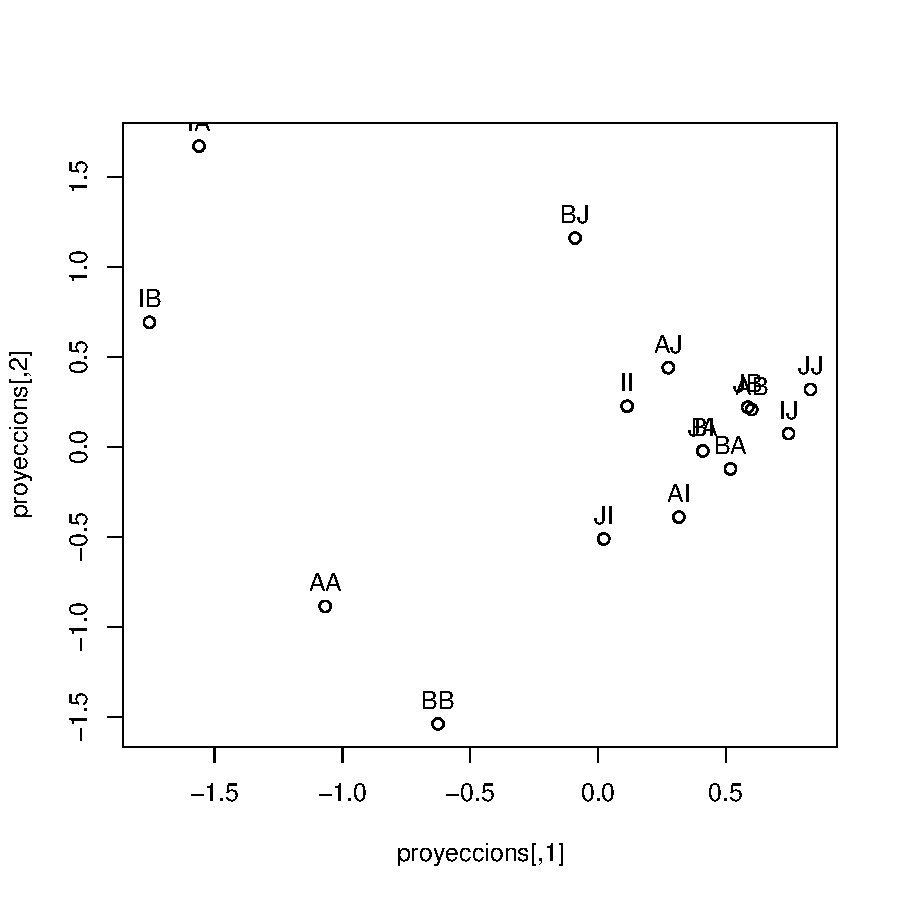
\includegraphics[scale=0.35]{AnCorrFiles.pdf}
\end{center}
}
\end{itemize}
\end{frame}
\subsection{Proyección de las columnas}
\begin{frame}
\frametitle{Proyección de las columnas}
\begin{itemize}
\item<2->{Vamos a realizar el mismo análisis de la matriz de frecuencias relativas $\vect{F}$ que hemos hecho anteriormente pero ahora por columnas.}
\item<3->{Consideramos las $J$ columnas como $J$ puntos en el espacio $\mathbb{R}^I$.}
\item<4->{El objetivo de nuestro análisis es buscar una representación de estos $J$ puntos en un espacio de dimensión menor que nos permita apreciar sus distancias relativas.}
\item<5->{Debemos tener en cuenta las mismas consideraciones que teníamos por filas.}
\end{itemize}
\end{frame}

\begin{frame}
\frametitle{Proyección de las columnas}
\begin{itemize}
\item<2->{Para obtener la mejor representación bidimensional de las filas de la tabla de contingencia, hay que seguir los pasos siguientes:
\begin{itemize}
\item<4->{Calcular la matriz $\vect{Z}\vect{Z}^\top$ y obtener sus vectores y valores propios. Los valores propios de la matriz anterior son los mismos que los valores propios de la matriz $\vect{Z}^\top\vect{Z}$ calculada anteriormente.}
\item<5->{Tomar los dos vectores propios, $\vect{w}_1$ y $\vect{w}_2$ ligados a los dos mayores valores propios menores que la unidad de esta matriz.}
\item<6->{Calcular las proyecciones siguientes $\vect{D}_c^{-1}\vect{F}^\top\vect{D}_f^{-1/2}\vect{w}_i$, $i=1,2$ y representarlas gráficamente en un espacio bidimensional.}
\end{itemize}}
\end{itemize}
\end{frame}

\begin{frame}
\frametitle{Ejemplo anterior}
\begin{itemize}
\item<2->{La matriz $\vect{Z}\vect{Z}^\top$ valdrá:
{\tiny
$$
\left(
\begin{array}{r@{}r@{}r@{}r@{}r@{}r@{}r@{}r@{}r@{}r@{}r@{}r@{}r@{}r@{}r@{}r}
0.25, &   0.02, &   0.07, &   0.02, &   0.02, &   0.24, &   0.04, &   0.00, &   0.06, &   0.15, &   0.06, &   0.00, &   0.04, &   0.02, &   0.10, &   0.00 \\
0.02, &   0.10, &   0.04, &   0.08, &   0.04, &   0.00, &   0.07, &   0.03, &   0.00, &   0.03, &   0.07, &   0.07, &   0.07, &   0.07, &   0.08, &   0.12 \\
0.07, &   0.04, &   0.12, &   0.06, &   0.09, &   0.12, &   0.06, &   0.04, &   0.00, &   0.00, &   0.08, &   0.07, &   0.06, &   0.07, &   0.03, &   0.08 \\
0.02, &   0.08, &   0.06, &   0.12, &   0.09, &   0.03, &   0.08, &   0.08, &   0.10, &   0.02, &   0.09, &   0.09, &   0.08, &   0.06, &   0.06, &   0.09 \\
0.02, &   0.04, &   0.09, &   0.09, &   0.16, &   0.06, &   0.12, &   0.02, &   0.00, &   0.03, &   0.03, &   0.09, &   0.12, &   0.06, &   0.03, &   0.04 \\
0.24, &   0.00, &   0.12, &   0.03, &   0.06, &   0.35, &   0.03, &   0.00, &   0.00, &   0.00, &   0.08, &   0.03, &   0.03, &   0.00, &   0.10, &   0.00 \\
0.04, &   0.07, &   0.06, &   0.08, &   0.12, &   0.03, &   0.14, &   0.02, &   0.00, &   0.05, &   0.03, &   0.05, &   0.14, &   0.09, &   0.05, &   0.04 \\
0.00, &   0.03, &   0.04, &   0.08, &   0.02, &   0.00, &   0.02, &   0.13, &   0.16, &   0.00, &   0.10, &   0.03, &   0.02, &   0.05, &   0.00, &   0.06 \\
0.06, &   0.00, &   0.00, &   0.10, &   0.00, &   0.00, &   0.00, &   0.16, &   0.35, &   0.17, &   0.10, &   0.00, &   0.00, &   0.00, &   0.00, &   0.00 \\
0.15, &   0.03, &   0.00, &   0.02, &   0.03, &   0.00, &   0.05, &   0.00, &   0.17, &   0.36, &   0.00, &   0.00, &   0.05, &   0.03, &   0.03, &   0.00 \\
0.06, &   0.07, &   0.08, &   0.09, &   0.03, &   0.08, &   0.03, &   0.10, &   0.10, &   0.00, &   0.14, &   0.07, &   0.03, &   0.06, &   0.06, &   0.13 \\
0.00, &   0.07, &   0.07, &   0.09, &   0.09, &   0.03, &   0.05, &   0.03, &   0.00, &   0.00, &   0.07, &   0.11, &   0.05, &   0.04, &   0.05, &   0.12 \\
0.04, &   0.07, &   0.06, &   0.08, &   0.12, &   0.03, &   0.14, &   0.02, &   0.00, &   0.05, &   0.03, &   0.05, &   0.14, &   0.09, &   0.05, &   0.04 \\
0.02, &   0.07, &   0.07, &   0.06, &   0.06, &   0.00, &   0.09, &   0.05, &   0.00, &   0.03, &   0.06, &   0.04, &   0.09, &   0.11, &   0.03, &   0.10 \\
0.10, &   0.08, &   0.03, &   0.06, &   0.03, &   0.10, &   0.05, &   0.00, &   0.00, &   0.03, &   0.06, &   0.05, &   0.05, &   0.03, &   0.11, &   0.07 \\
0.00, &   0.12, &   0.08, &   0.09, &   0.04, &   0.00, &   0.04, &   0.06, &   0.00, &   0.00, &   0.13, &   0.12, &   0.04, &   0.10, &   0.07, &   0.23
\end{array}
\right)
$$
}}
\item<3->{Los valores propios de la matriz anterior son:
$$
\begin{array}{r}
1.00,  0.57,  0.52,  0.37,  0.24,  0.12,  0.11,  0.00,\\  0.00,  0.00,  0.00,  0.00,  0.00,  0.00,  0.00,  0.00.
\end{array}
$$ Obsérvese que los valores propios no nulos ya estaban calculados al hacer el análisis por filas.}
\end{itemize}
\end{frame}

\begin{frame}
\frametitle{Ejemplo anterior}
\begin{itemize}
\item<2->{Los vectores propios correspondientes a los valores propios $0.57$ y $0.52$ son:
{\tiny $$
\vect{w}=\begin{pmatrix}
0.41 & 0.35 \\
-0.18 & -0.06 \\
-0.11 & 0.14 \\
-0.10 & -0.17 \\
-0.18 & 0.04 \\
0.24 & 0.61 \\
-0.14 & 0.01 \\
0.02 & -0.29 \\
0.46 & -0.51 \\
0.52 & -0.21 \\
-0.04 & -0.09 \\
-0.22 & -0.02 \\
-0.14 & 0.01 \\
-0.17 & -0.07 \\
-0.01 & 0.16 \\
-0.32 & -0.13 
\end{pmatrix}
$$}}
\end{itemize}
\end{frame}

\begin{frame}
\frametitle{Ejemplo anterior}
\begin{itemize}
\item<2->{La matriz $\vect{D}_c^{-1}\vect{F}^\top\vect{D}_f^{-1/2}$ vale en nuestro caso:
{\tiny
$$
\left(
\begin{array}{r@{}r@{}r@{}r@{}r@{}r@{}r@{}r@{}r@{}r@{}r@{}r@{}r@{}r@{}r@{}r}
0.00, &   0.00, &   0.00, &   0.70, &   0.00, &   0.00, &   0.00, &   1.10, &   1.80, &   0.00, &   0.70, &   0.00, &   0.00, &   0.00, &   0.00, &   0.00 \\
0.00, &   0.64, &   0.00, &   0.50, &   0.00, &   0.00, &   0.00, &   0.00, &   0.00, &   0.00, &   0.50, &   0.64, &   0.00, &   0.00, &   0.64, &   1.00 \\
0.00, &   0.00, &   0.49, &   0.44, &   0.98, &   0.44, &   0.49, &   0.00, &   0.00, &   0.00, &   0.00, &   0.56, &   0.49, &   0.00, &   0.00, &   0.00 \\
0.00, &   0.28, &   0.49, &   0.22, &   0.24, &   0.00, &   0.24, &   0.35, &   0.00, &   0.00, &   0.44, &   0.28, &   0.24, &   0.56, &   0.00, &   0.65 \\
0.32, &   0.41, &   0.00, &   0.32, &   0.36, &   0.00, &   0.71, &   0.00, &   0.00, &   0.41, &   0.00, &   0.00, &   0.71, &   0.41, &   0.41, &   0.00 \\
1.05, &   0.00, &   0.39, &   0.00, &   0.00, &   1.40, &   0.00, &   0.00, &   0.00, &   0.00, &   0.35, &   0.00, &   0.00, &   0.00, &   0.45, &   0.00 \\
0.87, &   0.00, &   0.00, &   0.00, &   0.00, &   0.00, &   0.00, &   0.00, &   1.13, &   2.25, &   0.00, &   0.00, &   0.00, &   0.00, &   0.00, &   0.00
\end{array}
\right)
$$
}
}
\item<3->{Las proyecciones $\vect{D}_c^{-1}\vect{F}^\top\vect{D}_f^{-1/2}\vect{w}$ calculadas por columnas valen:
$$
\begin{pmatrix}
0.75 & -1.43 \\
-0.65 & -0.21 \\
-0.43 & 0.29 \\
-0.61 & -0.24 \\
-0.10 & 0.01 \\
0.70 & 1.31 \\
2.03 & -0.75 
\end{pmatrix}
$$}
\end{itemize}
\end{frame}

\begin{frame}
\frametitle{Ejemplo anterior}
\begin{itemize}
\item<2->{La representación gráfica de las proyecciones anteriores es:
\begin{center}
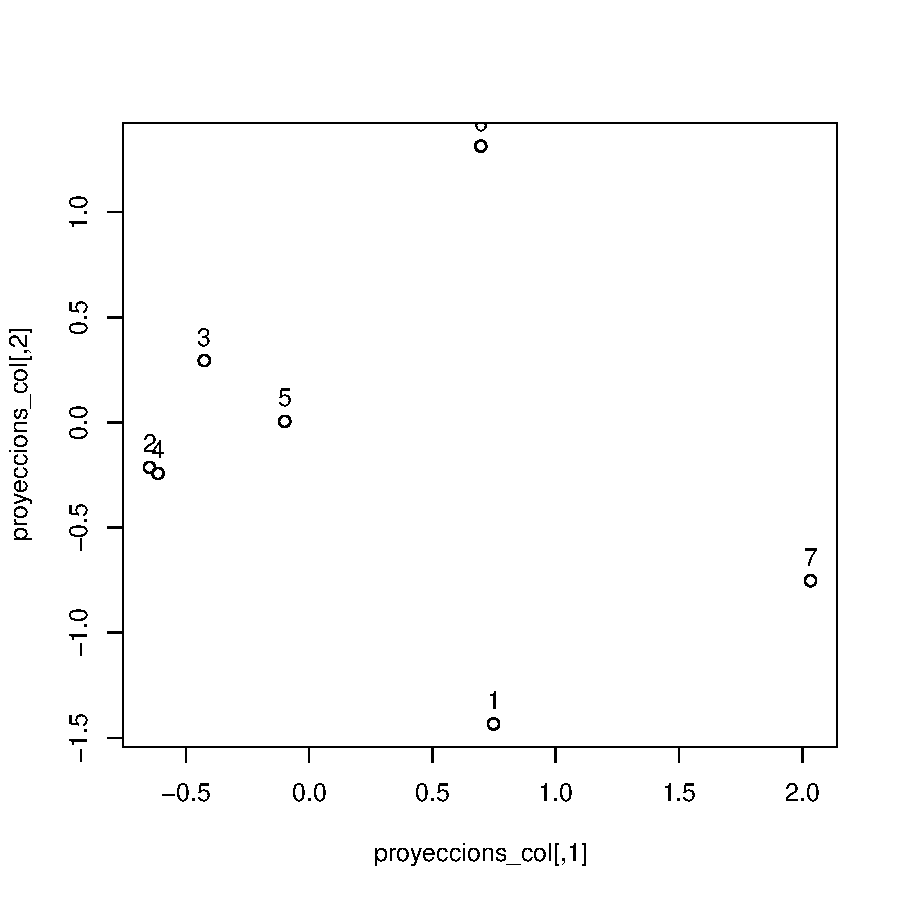
\includegraphics[scale=0.35]{AnCorrColumnes.pdf}
\end{center}}
\end{itemize}
\end{frame}
\begin{frame}
\frametitle{Ejemplo anterior}
\begin{itemize}
\item<2->{En el gráfico anterior se puede observar las similitudes o las diferencias del genotipo entre las crías de rata y las ratas adultas que las crían con diferente porcentaje de aumento de peso al cabo de 28 días. }
\item<3->{Por ejemplo, vemos que las crías de rata y ratas adultas con porcentaje de aumento de peso en segundo y en cuarto lugar tienen un genotipo muy parecido.}
\item<4->{En cambio, la mayor diferencia entre el genotipo de las crías y las ratas adultas se encuentra en las crías de rata con porcentaje de aumento de peso en primer y sexto lugar.}
\end{itemize}
\end{frame}
\subsection{Análisis conjunto}
\begin{frame}
\frametitle{Análisis conjunto}
\begin{itemize}
\item<2->{Debido a la simetría del problema, conviene representar conjuntamente las proyecciones de las filas y las columnas en el mismo gráfico.}
\item<3->{Antes de dar los pasos para hacer tal representación conviene tener en cuenta que
\begin{itemize}
\item<4->{si $\vect{v}$ es vector propio de la matriz $\vect{Z}^\top\vect{Z}$ de valor propio $\lambda$, entonces $\vect{Z}\vect{v}$ es vector propio de la matriz $\vect{Z}\vect{Z}^\top$ del mismo valor propio y} \item<5->{viceversa: si $\vect{w}$ es vector propio de la matriz $\vect{Z}\vect{Z}^\top$ de valor propio $\lambda$, entonces $\vect{Z}^\top\vect{w}$ es vector propio de la matriz $\vect{Z}^\top\vect{Z}$ del mismo valor propio.}
\end{itemize}}
\end{itemize}
\end{frame}

\begin{frame}
\frametitle{Análisis conjunto}
\begin{itemize}
\item<2->{Para hacer la representación conjunta de las proyecciones de las filas y las columnas hay que realizar los pasos siguientes:\begin{itemize}
\item<3->{Se calcula la matriz de frecuencias relativa $\vect{F}$.}
\item<4->{Se calcula la matriz estandarizada $\vect{Z}$.}
\item<5->{Se busca de las dos matrices siguientes, $\vect{Z}^\top\vect{Z}$ o  $\vect{Z}\vect{Z}^\top$ la que tenga menor dimensión. Supongamos para fijar ideas que es la matriz $\vect{Z}^\top\vect{Z}$. Se calculan los dos valores propios menores que~$1$ más grandes de la matriz anterior. Sean $\vect{v}_1$ y $\vect{v}_2$ los dos vectores propios asociados a los dos valores propios anteriores. La proyección de las filas vendrá dada por $\vect{D}_f^{-1/2}\vect{Z}\vect{v}_i$, $i=1,2$.}
\item<6->{Sean $\vect{w}_i = \vect{Z}\vect{v}_i$, $i=1,2$ los vectores propios de la matriz $\vect{Z}\vect{Z}^\top$ asociados a los valores propios anteriores. La proyección de las columnas vendrá dada por: 
$\vect{D}_c^{-1/2}\vect{Z}^\top\vect{w}_i$, $i=1,2$.} 
\end{itemize}}
\end{itemize}
\end{frame}

\begin{frame}
\frametitle{Ejemplo anterior}
\begin{itemize}
\item<2->{En el ejemplo anterior la matriz de menor dimensión era $\vect{Z}^\top\vect{Z}$ ($7\times 7$).}
\item<3->{Los valores propios a considerar eran: $0.57$ y $0.52$.}
\item<4->{Los vectores propios eran:$$
\begin{pmatrix}
-0.28 & 0.57 \\
0.29 & 0.10 \\
0.20 & -0.15 \\
0.42 & 0.17 \\
0.06 & -0.00 \\
-0.37 & -0.74 \\
-0.69 & 0.27 
\end{pmatrix}
$$}
\end{itemize}
\end{frame}

\begin{frame}
\frametitle{Ejemplo anterior}
\begin{itemize}
\item<2->{La proyección de las filas era:{\tiny $$
\vect{v}=\begin{pmatrix}
-1.07 & -0.89 \\
0.60 & 0.21 \\
0.32 & -0.39 \\
0.28 & 0.44 \\
0.52 & -0.12 \\
-0.63 & -1.54 \\
0.41 & -0.02 \\
-0.09 & 1.16 \\
-1.56 & 1.67 \\
-1.75 & 0.69 \\
0.11 & 0.23 \\
0.75 & 0.07 \\
0.41 & -0.02 \\
0.59 & 0.22 \\
0.02 & -0.51 \\
0.83 & 0.32 
\end{pmatrix}
$$}
}
\end{itemize}
\end{frame}
\begin{frame}
\frametitle{Ejemplo anterior}
\begin{itemize}
\item<2->{Busquemos ahora los vectores propios de la matriz $\vect{Z}\vect{Z}^\top$: $\vect{w}_i = \vect{Z}\vect{v}_i$, donde $\vect{v}_i$ son los vectores propios hallados anteriormente por columnas:
{\tiny $$
\vect{w}=\begin{pmatrix}
-0.31 & -0.25 \\
0.13 & 0.05 \\
0.08 & -0.10 \\
0.08 & 0.13 \\
0.13 & -0.03 \\
-0.18 & -0.44 \\
0.10 & -0.01 \\
-0.02 & 0.21 \\
-0.35 & 0.37 \\
-0.39 & 0.15 \\
0.03 & 0.06 \\
0.17 & 0.02 \\
0.10 & -0.01 \\
0.13 & 0.05 \\
0.00 & -0.11 \\
0.24 & 0.09 \\
\end{pmatrix}
$$}}
\end{itemize}
\end{frame}

\begin{frame}
\frametitle{Ejemplo anterior}
\begin{itemize}
\item<2->{Las proyecciones de las columnas será la matriz $\vect{D}_c^{-1/2}\vect{Z}^\top\vect{w}$:
$$\begin{pmatrix}
-0.56 & 1.03 \\
0.49 & 0.15 \\
0.32 & -0.21 \\
0.46 & 0.17 \\
0.07 & -0.00 \\
-0.52 & -0.95 \\
-1.53 & 0.54 \\
\end{pmatrix}$$
}
\end{itemize}
\end{frame}
\begin{frame}
\frametitle{Ejemplo anterior}
\begin{itemize}
\item<2->{En el gráfico siguiente se puede ver la proyección conjunta donde en rojo están las proyecciones por filas y en negro, las proyecciones por columnas:
\begin{center}
\includegraphics[scale=0.5]{AnCorrConjunta.pdf}
\end{center}}
\end{itemize}
\end{frame}

\part{Clasificación} 


%\part{Métodos de clasificación automática.}
%\frame{\partpage}

\chapter{Métodos de clasificación automática}

\section{Introducción}
\begin{frame}
\frametitle{Descripción del problema}
\begin{itemize}
\item<2->{Tenemos un conjunto de individuos con unas ciertas medidas multidimensionales.}
\item<3->{Queremos ver si existe una "forma natural" de clasificar a dichos individuos en grupos.}
\item<4->{Los grupos que formemos tienen que ser lo más homogéneos posible y las diferencias entre los grupos, lo más acentuadas posible.}
\end{itemize}
\end{frame}

\section{Algoritmo de las $k$-medias}
\begin{frame}
\frametitle{Introducción al algoritmo de las $k$-medias}
\begin{itemize}
\item<2->{En todo método de partición, partimos de $n$ individuos de los que se han tomado $p$ mediciones. O sea, tenemos una matriz $n\times p$ de $n$ individuos con $p$ variables:
$\vect{X}=
\begin{pmatrix}
x_{11}&x_{12}&\ldots&x_{1p} \\ 
x_{21}&x_{22}&\ldots&x_{2p} \\
\vdots&\vdots&\vdots&\vdots \\
x_{n1}&x_{n2}&\ldots&x_{no}
\end{pmatrix}$}
\item<3->{El objetivo del algoritmo de las $k$-medias es dividir los $n$ individuos en un número de conjuntos o grupos prefijado~$G$.}
\end{itemize}
\end{frame}

\section{Algoritmo de las $k$-medias}
\begin{frame}
\frametitle{Etapas del algoritmo de las $k$-medias}
\begin{itemize}
\item<2->{Se seleccionan $G$ puntos como centros de los puntos iniciales. Hay distintas formas de realizar dicha selección:
\begin{itemize}
\item asignando aleatoriamente los objetos a los grupos y tomando los centros de los grupos formados,
\item tomando como centros los $G$ más alejados entre sí,
\item seleccionando los centros ``a priori".
\end{itemize}}
\item<3->{Calcular las distancias euclídeas de cada elemento a los centros de los $G$ grupos, y asignar cada elemento al grupo de cuyo centro esté más próximo. La asignación se realiza secuencialmente y al introducir un nuevo elemento en un grupo se recalculan las coordenadas del nuevo centro del grupo.}
\item<4->{Definir un criterio de optimalidad y comprobar si reasignando alguno de los elementos mejora el criterio.}
\item<5->{Si no es posible mejorar el criterio de optimalidad, terminar el proceso.}
\end{itemize}
\end{frame}
\begin{frame}
\frametitle{Criterio de optimalidad.}
\begin{itemize}
\item<2->{Sea $x_{ijg}$ la medida $j$-ésima del individuo $i$-ésimo que pertenece al grupo~$g$. Definimos la suma de cuadrados dentro de los grupos $SCDG$ como:
$$
SCDG = \sum_{g=1}^G\sum_{j=1}^p\sum_{i=1}^{n_g} (x_{ijg}-\overline{x}_{jg})^2,
$$
donde $\overline{x}_{jg}$ es la media de esta variable en el grupo~$g$ y $n_g$ representa el número de elementos de grupo~$g$.}
\item<3->{Nuestro objetivo será encontrar aquella partición que minimice $SCDG$.}
\item<4->{La suma de cuadrados $SCDG$ puede escribirse como:
$$
SCDG = \sum_{g=1}^G\sum_{j=1}^{p}  n_g s_{jg}^2,
$$
donde $s_{jg}^2$ es la varianza de la variable $j$ en el grupo~$g$.}
\end{itemize}
\end{frame}

\begin{frame}
\frametitle{Criterio de optimalidad.}
\begin{itemize}
\item<2->{Escribamos matricialmente el criterio de optimalidad:
$$
SCDG = \sum_{g=1}^G\sum_{i=1}^{n_g} (\vect{x}_{ig}-\overline{\vect{x}}_g)^\top (\vect{x}_{ig}-\overline{\vect{x}}_g),
$$
donde $\vect{x}_{ig}$ sería el vector de los $j$ valores del individuo $i$-ésimo dentro del grupo~$g$ y $\overline{\vect{x}}_g$ sería el vector de medias de los $g$ grupos.}
\item<3->{El valor anterior de dentro del sumatorio es la distancia euclídea entre el individuo $i$-ésimo dentro del grupo $g$ y la media dentro del grupo~$g$. Si nombramos $d^2(i,g)$ a dicha distancia, podemos escribir: $$SCDG=\sum_{g=1}^G\sum_{i=1}^{n_g} d^2(i,g).$$}
\end{itemize}
\end{frame}
\begin{frame}
\frametitle{Criterio de optimalidad.}
\begin{itemize}
\item<2->{Usando que $ (\vect{x}_{ig}-\overline{\vect{x}}_g)^\top (\vect{x}_{ig}-\overline{\vect{x}}_g) =tr( (\vect{x}_{ig}-\overline{\vect{x}}_g) (\vect{x}_{ig}-\overline{\vect{x}}_g))^\top$ (ejercicio), podemos escribir la suma de cuadrados como:
$$
SCDG=tr\left( \sum_{g=1}^G\sum_{i=1}^{n_g} (\vect{x}_{ig}-\overline{\vect{x}}_g) (\vect{x}_{ig}-\overline{\vect{x}}_g))^\top \right),
$$
donde $tr$ significa traza.}
\item<3->{Nombrando $\vect{W}$ a la matriz $ \sum_{g=1}^G\sum_{i=1}^{n_g} (\vect{x}_{ig}-\overline{\vect{x}}_g) (\vect{x}_{ig}-\overline{\vect{x}}_g))^\top$, tenemos que el criterio de optimalidad equivale a minimizar la traza de la matriz~$\vect{W}$.}
\end{itemize}
\end{frame}

\begin{frame}
\frametitle{Ejemplo}
\begin{itemize}
\item<2->{La siguiente tabla muestra el gasto medio en varios tipos de comida para distintos tipos de familias en Francia: trabajadores manuales (TM), empleados (EM) y directivos (DIR) con distintos número de hijos: 2, 3, 4 o 5 hijos.

Significado de las siglas:
\begin{description}
\item[TF] Tipo familia
\item[P] Pan
\item[VE] Vegetales
\item[F] Fruta
\item[C] Carne
\item[A] Aves
\item[L] Leche
\item[VI] Vino
\end{description}
}
\end{itemize}
\end{frame}
\begin{frame}
\frametitle{Ejemplo}
\begin{itemize}
\item<2->{\begin{tabular}{|r|r|r|r|r|r|r|r|}
\hline
TF&P&VE&F&C&A&L&VI\\\hline
TM2&332&428&354&1437&526&247&427\\\hline
EM2&293&559&388&1527&567&239&258\\\hline
DIR2&372&767&562&1948&927&235&433\\\hline
TM3&406&563&341&1507&544&324&407\\\hline
EM3&386&608&396&1501&558&319&363\\\hline
DIR3&438&843&689&2345&1148&243&341\\\hline
TM4&534&660&367&1620&638&414&407\\\hline
EM4&460&699&484&1856&762&400&416\\\hline
DIR4&385&789&621&2366&1149&304&282\\\hline
TM5&655&776&423&1848&759&495&486\\\hline
EM5&584&995&548&2056&893&518&319\\\hline
DIR5&515&1097&887&2630&1167&561&284\\\hline
\end{tabular}}
\end{itemize}
\end{frame}
\begin{frame}
\frametitle{Ejemplo}
\begin{itemize}
\item<2->{Elegiremos $G=3$. Elegiremos como centros de los valores iniciales las medias de los $4$ primeros individuos, luego las medias de los individuos $5$ al $8$ y por último las medias de los individuos $9$ al $12$. O sea, elegimos como grupos iniciales los siguientes:
Grupo 1: individuos $1$, $2$, $3$ y $4$. Grupo 2: individuos $5$, $6$, $7$ y $8$ y Grupo 3: individuos $9$, $10$, $11$ y $12$. Las coordenadas de los $3$ centros iniciales son las siguientes:
$$
{\small \begin{pmatrix}
350.75 & 579.25 & 411.25 & 1604.75 & 641.0 & 261.25 & 381.25 \\
454.50 & 702.50 & 484.00 & 1830.50 & 776.5 & 344.00 & 381.75 \\
534.75 & 914.25 & 619.75 & 2225.00 & 992.0 & 469.50 & 342.75 \\
\end{pmatrix}}
$$}
\end{itemize}
\end{frame}
\begin{frame}
\frametitle{Ejemplo}
\begin{itemize}
\item<2->{En el gráfico siguiente observamos la proyección de las dos primeras variables de los individuos junto con los centros de los grupos iniciales (en rojo):
\vskip0.25cm
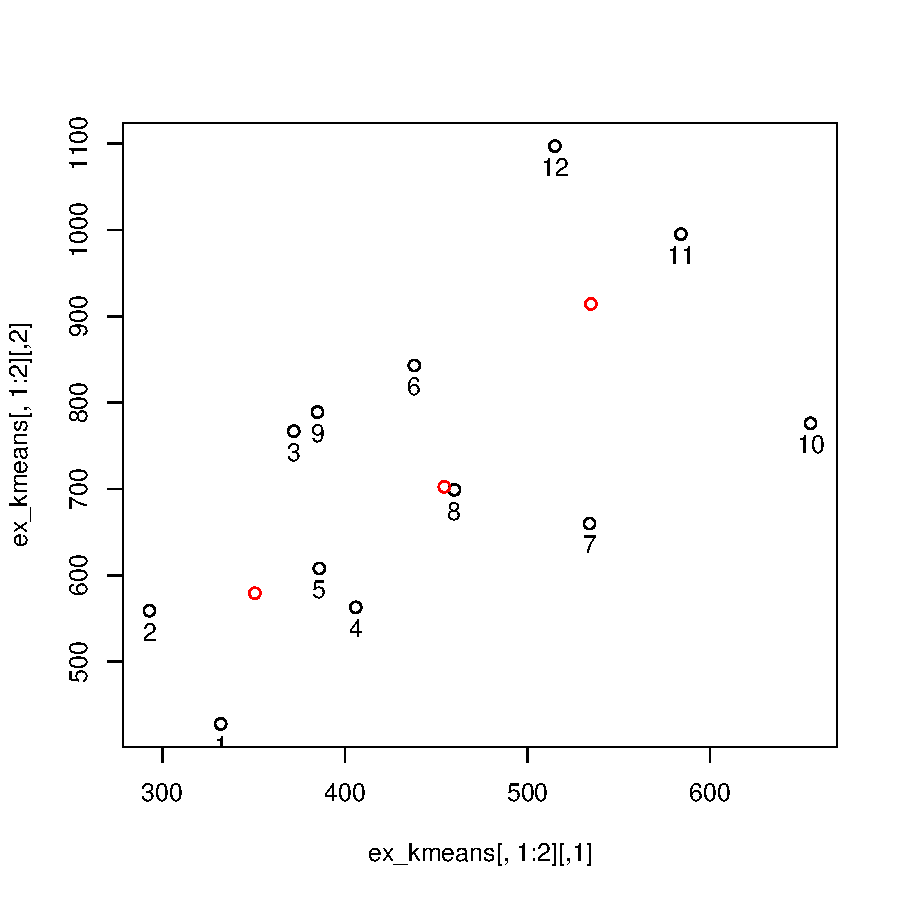
\includegraphics[scale=0.4]{kmeans1.pdf}}
\end{itemize}
\end{frame}
\begin{frame}
\frametitle{Ejemplo}
\begin{itemize}
\item<-2>{Vamos a aplicar el algoritmo de k-means a nuestro ejemplo. El valor inicial de $SCDG$ es $1916875$. Calculemos primero el grupo más cercano de cada individuo hallando la distancia entre éste y el centro correspondiente:
\begin{itemize}
\item Individuo 1: distancias de $(332,428,354,1437,526,247,427)$ a cada uno de los centros: 
$$
{\tiny
\begin{array}{rl}
d((332,428,\ldots ,427), (350.75, 579.25 ,\ldots , 381.25)) = & 264.895, \\
d((332,428,\ldots ,427), (454.50, 702.50 , \ldots , 381.75 ) = & 579.945, \\
d((332,428,\ldots ,427), (534.75, 914.25, \ldots , 342.75 ) = & 1114.883.
\end{array}}$$
Por tanto, el grupo correspondiente al primer individuo es el primero. No hay ningún cambio.
\item Con el individuo 2, tampoco hay cambios. En cambio con el individuo 3, resulta que el grupo más cercano es el grupo~2. Por tanto, cambiamos los grupos por: 
$$
G1 = \{ 1,2,4\},\ G2 = \{3,5,6,7,8\},\ G3 = \{ 9,10,11,12\}.
$$
\end{itemize}
}
\end{itemize}
\end{frame}

\begin{frame}
\frametitle{Ejemplo}
\begin{itemize}
\item<2->{El nuevo valor de $SCDG$ es $1622739$. Ha habido por tanto una mejora. Los nuevos centros son:
$$
{\tiny \begin{pmatrix}
343.667 & 516.667 & 361.000 &  1490.333 &  545.667 & 270.000 &  364.000 \\
438.000 & 715.400 &  499.600 & 1854.000 &  806.600 &  322.200 &  392.000  \\
534.750 & 914.250 &  619.750 &  2225.000 &  992.000 & 469.500 &  342.750 \\
\end{pmatrix}}
$$}
\item<3->{Volvemos a mirar el grupo más cercano de cada individuo: individuo 1: grupo 1 (no hay cambios); individuo 2: grupo 1 (no hay cambios); individuo 3: grupo 2 (no hay cambios); individuo 4:  grupo 1 (no hay cambios); individuo 5: grupo 1. Por tanto, cambiamos los grupos por: 
$$
G1 = \{ 1,2,4,5\},\ G2 = \{3,6,7,8\},\ G3 = \{ 9,10,11,12\}.
$$
El nuevo valor de $SCDG$ es $1367967$. Se sigue mejorando. Los nuevos centros son:
$$
{\tiny \begin{pmatrix}
354.250 &  539.500 &  369.750 &  1493.000 &  548.750 &  282.250 &  363.750 \\
451.000 &  742.250 &  525.500 &  1942.250 &  868.750 &  323.000 &  399.250 \\
534.75 & 914.250 &  619.750 &  2225.000 &  992.000 &  469.500 & 342.750 \\
\end{pmatrix}}
$$}
\end{itemize}
\end{frame}

\begin{frame}
\frametitle{Ejemplo}
\begin{itemize}
\item<2->{La tabla siguiente va mostrando los pasos del algoritmo donde la primera columna nos indica el individuo que va cambiando de grupo:
\begin{center}
{\tiny\begin{tabular}{|c|c|c|c|l|}\hline
&Grupo 1& Grupo 2& Grupo 3&$SCDG$\\\hline
$6$&$\{1,2,4,5\}$&$\{3,7,8\}$&$\{6,9,10,11,12\}$&$1072675$\\\hline
$10$&$\{1,2,4,5\}$&$\{3,7,8,10\}$&$\{6,9,11,12\}$&$709037.8$\\\hline
$11$&$\{1,2,4,5\}$&$\{3,7,8,10,11\}$&$\{6,9,12\}$&$632336.1$\\\hline
$7$&$\{1,2,4,5,7\}$&$\{3,8,10,11\}$&$\{6,9,12\}$&$564800.9$\\\hline
\end{tabular}}
\end{center}}
\end{itemize}
\end{frame}
\subsection{Propiedades del algoritmo de $k$-means}
\begin{frame}
\frametitle{Propiedades del algoritmo de $k$-means}
\begin{itemize}
\item<2->{El algoritmo no es invariante ante cambios de escala. Por tanto, si las variables van en unidades distintas, conviene estandarizarlas antes de aplicar el algoritmo.}
\item<3->{El algoritmo produce grupos aproximadamente esféricos ya que tiende a minimizar las distancias euclídeas entre los puntos y sus medias de grupo.}
\end{itemize}
\end{frame}

\subsection{Elección del número de grupos}
\begin{frame}
\frametitle{Elección del número de grupos}
\begin{itemize}
\item<2->{El procedimiento habitual de elegir cuántos grupos hay que usar en el algoritmo de $k$-means es el llamado test $F$ de reducción de variabilidad.}
\item<3->{Dicho test consiste en calcular:
$$
F=\frac{SCDG(G)-SCDG(G+1)}{SCDG(G+1)/(n-G-1)},
$$
donde se compara la variabilidad al aumentar un grupo con la varianza promedio. El valor obtenido se compara con el valor crítico de una distribución $F$ de $p$ y $p(n-G-1)$ grados de libertad. Hay que decir que dicha regla no está muy justificada ya que los datos no tienen porqué verificar las hipótesis necesarias para aplicar la distribución~$F$.}
\end{itemize}
\end{frame}
\begin{frame}
\frametitle{Ejemplo}
\begin{itemize}
\item<2->{En la tabla siguiente observamos los valores de $SCDG$ para distintas elecciones de $G$:
\begin{center}
\begin{tabular}{|c|c|c|}\hline
$G$&$SCDG$&$F$\\\hline
$3$&$564800.9$& \\\hline
$4$&$363066.1$&$\frac{(564800.9-363066.1)}{363066.1/(12-3-1)}=4.44$\\\hline
$5$&$255134.8$&$\frac{(363066.1-255134.8)}{255134.8/(12-4-1)}=2.96$\\\hline
$6$&$153977.9$&$\frac{(255134.8-153977.9)}{153977.9/(12-5-1)}=3.94$\\\hline
$7$&$109217.7$&$\frac{153977.9-109217.7}{109217.7/(12-6-1)}=2.05$\\\hline
\end{tabular}
\end{center}}
\item<3->{La reducción de la variabilidad más acentuada se produce al pasar de $3$ a $4$ grupos. Si hallamos el valor crítico (para $\alpha =0.05$) de la distribución $F$ con $p=7$ y $p(n-G-1)=7\cdot (12-3-1)=56$ grados de libertad, obtenemos $F_{0.95,7,56}=2.18$. Como $4.44 > 2.18$, concluimos que la variabilidad se ha reducido y, según este criterio, escogeríamos $G=4$ como el número de grupos óptimo.}
\end{itemize}
\end{frame}
\section{Métodos jerárquicos}

\begin{frame}
\frametitle{Introducción}
\begin{itemize}
\item<2->{Los métodos jerárquicos parten de una matriz de distancias o similaridades. O sea, suponemos que tenemos una matriz $D$ $n\times n$ que nos dice la distancia entre los individuos o elementos de la muestra: $d_{ij}:$ distancia entre el individuo~$i$ y el individuo~$j$. }
\item<3->{A partir de la matriz de distancias, se define el algoritmo de construcción de grupos. O sea, usando la matriz de distancias definida anteriormente, indicar cómo se formarán los distintos grupos.}
\end{itemize}
\end{frame}
\subsection{Matriz de distancias}
\begin{frame}
\frametitle{Cómo calcular la matriz de distancias}
\begin{itemize}
\item<2->{Recordemos que tenemos $n$ individuos de los que se han tomado $p$ mediciones:
$\vect{X}=
\begin{pmatrix}
x_{11}&x_{12}&\ldots&x_{1p} \\ 
x_{21}&x_{22}&\ldots&x_{2p} \\
\vdots&\vdots&\vdots&\vdots \\
x_{n1}&x_{n2}&\ldots&x_{np}
\end{pmatrix}$}
\item<3->{A partir de la matriz $\vect{X}$ hemos de construir una matriz de similaridad-disimilaridad $\vect{D}$ $n\times n$ entre los objetos:
$\vect{D}=
\begin{pmatrix}
d_{11}&d_{12}&\ldots&d_{1n} \\ 
d_{21}&d_{22}&\ldots&d_{2p} \\
\vdots&\vdots&\vdots&\vdots \\
d_{n1}&d_{n2}&\ldots&d_{nn}
\end{pmatrix}$}
\item<4->{En el  caso en que $\vect{D}$ sea una matriz de similaridad, cuánto menor sean los valores $d_{ij}$, más alejados estarán los individuos $i$ y $j$ y en el segundo caso, más cercanos estarán.}
\end{itemize}
\end{frame}
\subsection{Datos binarios}
\begin{frame}
\frametitle{Introducción}
\begin{itemize}
\item<2->{Supongamos que la matriz $\vect{X}$ sólo coge los valores $0$ o $1$. En este caso, diremos que la estructura de los datos es binaria.}
\item<3->{De cara a definir la matriz de similaridad, consideremos los datos referentes al individuo~$i$ (columna $i$ de la matriz $\vect{X}$: $(x_{i1},\ldots,x_{ip})^\top$) y al individuo~$j$ (columna $j$ de la matriz $\vect{X}$: $(x_{j1},\ldots,x_{jp})^\top$)}
\item<4->{Definimos las cantidades siguientes:
$$
\begin{array}{rl}
a_1 = & \sum_{k=1}^p \mathcal{I}(x_{ik}=x_{jk}=1), \\
a_2 = & \sum_{k=1}^p \mathcal{I}(x_{ik}=0, x_{jk}=1), \\
a_3 = & \sum_{k=1}^p \mathcal{I}(x_{ik}=1, x_{jk}=0), \\
a_4 = & \sum_{k=1}^p \mathcal{I}(x_{ik}=x_{jk}=0),
\end{array}
$$
donde $\mathcal{I}(\mbox{condición})$ cuenta cuantos elementos de la matriz $\vect{X}$ cumplen la condición.}
\end{itemize}
\end{frame}
\begin{frame}
\frametitle{Definición de la matriz de distancias}
\begin{itemize}
\item<2->{Definimos la similaridad entre los individuos $i$ y $j$ como:
$$
d_{ij}=\frac{a_1 + \delta a_4}{a_1 + \delta a_4 +\lambda (a_2 + a_3)}.
$$
}
\item<3->{Los parámetros $\delta$ y $\lambda$ son factores de peso. La tabla siguiente muestra ejemplos de similaridades más comunes:
\vskip 0.25cm
\begin{tabular}{|l|r|r|c|}
\hline
Nombre&$\delta$&$\lambda$&Definición\\\hline
Jaccard&$0$&$1$&$\frac{a_1}{a_1 + a_2 +a_3}$ \\\hline
Tanimoto&$1$&$2$&$\frac{a_1+a_4}{a_1+2(a_2+a_3)+a_4}$\\\hline
Simple&$1$&$1$&$\frac{a_1 + a_4}{p}$\\\hline
Rusell y Rao&-&-&$\frac{a_1}{p}$\\\hline
Dice&$0$&$0.5$&$\frac{2a_1}{2a_1 + a_2 +a_3}$ \\\hline
Kulczynski&-&-&$\frac{a_1}{a_2 + a_3}$\\\hline
\end{tabular}}
\end{itemize}
\end{frame}
\begin{frame}
\frametitle{¿Por qué no se usa la distancia euclídea?}
\begin{itemize}
\item<2->{La distancia euclídea no sería adecuada en este caso ya que trata los valores $0$ y $1$ de la misma forma y en la mayoría de aplicaciones donde se tratan datos binarios, deben ser tratados de formas distintas.}
\item<3->{Por ejemplo, si $x_{ik}=1$ significa que el individuo $i$ tiene un cierto conocimiento sobre el lenguaje~$k$ y si $x_{ik}=0$ significa que no lo tiene, el valor $x_{ik}=0$ tiene que tratarse de forma distinta del valor $x_{ik}=1$.}
\end{itemize}
\end{frame}
\begin{frame}
\frametitle{Ejemplo}
\begin{itemize}
\item<2->{Consideremos $3$ tipos de marca de automóviles, Renault, Rover y Toyota. Se ha realizado una encuesta en $40$ personas para que opinen de las variables siguientes: Economía (EC), servicio (SER), valor no depreciado (V), precio (P)(valor $1$ para los coches más baratos), diseño (DI), deportividad (DE), seguridad (SEG) y facilidad de Manejo (FM). Los resultados van de $1$ (muy bueno) a $6$ (muy malo).}
\item<3->{Las medias de las valoraciones de los $40$ encuestados son:
\vskip 0.25cm
\begin{tabular}{|l|c|c|c|c|c|c|c|c|}
\hline
Modelo&EC&SER&V&P&DI&DE&SEG&FM\\\hline
Renault&2.7&3.3&3.4&3.0&3.1&3.4&3.0&2.7\\\hline
Rover&3.9&2.8&2.6&4.0&2.6&3.0&3.2&3.0\\\hline
Toyota&2.5&2.9&3.4&3.0&3.2&3.1&3.2&2.8\\\hline
\end{tabular}
}
\end{itemize}
\end{frame}
\begin{frame}
\frametitle{Ejemplo}
\begin{itemize}
\item<2->{Sea $\vect{X}$ la matriz de datos anterior:
$$
\vect{X}=
\begin{pmatrix}
2.7&3.3&3.4&3.0&3.1&3.4&3.0&2.7\\
3.9&2.8&2.6&4.0&2.6&3.0&3.2&3.0\\
2.5&2.9&3.4&3.0&3.2&3.1&3.2&2.8
\end{pmatrix}
$$
Se trata de una matriz $3\times 8$ de $3$ individuos con $8$ variables.}
\item<3->{A partir de la matriz anterior, construimos la matriz binaria siguiente:
$y_{ik}=\left\{\begin{array}{ll}
1,&\mbox{si } x_{ik}> \overline{x}_k, \\
0,&\mbox{en caso contrario.}
\end{array}
\right.$}
\item<4->{La matriz $\vect{Y}$ es:
$$
\vect{Y}=
\begin{pmatrix}
 0  &  1  &  1 &   0  &  1  &  1  &  0  &   0  \\
  1  &   0  &   0  &   1  &   0  &   0 &    1 &    1 \\
  0  &   0  &   1  &   0  &   1  &   0 &    1  &   0\\
\end{pmatrix}
$$
}
\end{itemize}
\end{frame}
\begin{frame}
\frametitle{Ejemplo}
\begin{itemize}
\item<2->{Si aplicamos la medida de Jaccard, obtenemos la matriz siguiente de similaridad:
$$
\vect{D}=
\begin{pmatrix}
1.000 & 0.000 & 0.400 \\
&1.000 & 0.167 \\
&&1.000
\end{pmatrix}
$$
}
\item<3->{La medida de Tanimoto da el siguiente resultado:
$$
\vect{D}=
\begin{pmatrix}
1.000 & 0.000 & 0.455 \\
&1.000 & 0.231 \\
&&1.000
\end{pmatrix}
$$}
\item<4->{La medida simple da como matriz de similaridad:
$$
\vect{D}=
\begin{pmatrix}
1.000 & 0.000 & 0.625 \\
&1.000 & 0.375 \\
&&1.000
\end{pmatrix}
$$}
\end{itemize}
\end{frame}
\subsection{Datos continuos}
\begin{frame}
\frametitle{Introducción}
\begin{itemize}
\item<2->{En el caso general de datos continuos, se usan las distancias generadas por las normas $L_r,\ r\geq 1$. Esto es, la distancia entre el individuo $i$ (fila $i$ de la matriz $\vect{X}$: $(x_{i1},\ldots,x_{ip})^\top$) y al individuo~$j$ (fila $j$ de la matriz $X$: $(x_{j1},\ldots,x_{jp})^\top$) viene dada por:
$$
d_{ij}=||\vect{x_i} - \vect{x_j}||_r = \left(\sum_{k=1}^p |x_{ik} - x_{jk}|^r\right)^{\frac{1}{r}}.
$$
}
\item<3->{Es claro que en este caso $d_{ii}=0$. Por tanto, usamos una matriz de distancias o disimilaridad. Si $r=2$, tenemos la distancia euclídea usual.}
\end{itemize}
\end{frame}
\begin{frame}
\frametitle{Escalado de los datos}
\begin{itemize}
\item<2->{Una suposición usual es que los datos estén en la misma escala. Si no fuese el caso, la definición de la matriz de distancias se realiza mediante una métrica $\vect{A}$. En el caso de la distancia euclídea, la modificación sería: 
$$
d_{ij}^2=||\vect{x_i} - \vect{x_j}||_\vect{A} = (\vect{x_i} - \vect{x_j})^\top \vect{A} (\vect{x_i} - \vect{x_j}).
$$}
\item<3->{La métrica $\vect{A}$ más usada es la siguiente: 
$$
\vect{A}= \mbox{diag} \left( s_{\vect{x_1}\vect{x_1}}^{-1},\ldots,s_{\vect{x_p}\vect{x_p}}^{-1}
\right),
$$
donde $s_{\vect{x_k}\vect{x_k}}$ es la varianza de la variable $k$-ésima.}
\item<4->{La distancia euclídea quedará de la forma siguiente:
$$
d_{ij}^2 = \sum_{k=1}^p \frac{\left(x_{ik}-x_{jk}\right)^2}{s_{\vect{x_k}\vect{x_k}}}.
$$}
\end{itemize}
\end{frame}
\begin{frame}
\frametitle{Ejemplo}
\begin{itemize}
\item<2->{Recordemos el ejemplo del gasto medio en varios tipos de comida para distintos tipos de familias en Francia: trabajadores manuales (TM), empleados (EM) y directivos (DIR) con distintos número de hijos: 2, 3, 4 o 5 hijos.

Significado de las siglas:
\begin{description}
\item[TF] Tipo familia
\item[P] Pan
\item[VE] Vegetales
\item[F] Fruta
\item[C] Carne
\item[A] Aves
\item[L] Leche
\item[VI] Vino
\end{description}
}
\end{itemize}
\end{frame}
\begin{frame}
\frametitle{Ejemplo}
\begin{itemize}
\item<2->{\begin{tabular}{|r|r|r|r|r|r|r|r|}
\hline
TF&P&VE&F&C&A&L&VI\\\hline
TM2&332&428&354&1437&526&247&427\\\hline
EM2&293&559&388&1527&567&239&258\\\hline
DIR2&372&767&562&1948&927&235&433\\\hline
TM3&406&563&341&1507&544&324&407\\\hline
EM3&386&608&396&1501&558&319&363\\\hline
DIR3&438&843&689&2345&1148&243&341\\\hline
TM4&534&660&367&1620&638&414&407\\\hline
EM4&460&699&484&1856&762&400&416\\\hline
DIR4&385&789&621&2366&1149&304&282\\\hline
TM5&655&776&423&1848&759&495&486\\\hline
EM5&584&995&548&2056&893&518&319\\\hline
DIR5&515&1097&887&2630&1167&561&284\\\hline
\end{tabular}}
\end{itemize}
\end{frame}
\begin{frame}
\frametitle{Ejemplo}
\begin{itemize}
\item<2->{La matriz de distancia euclidea para los datos anteriores es:
%\vskip 0.25cm
%\includegraphics[scale=0.7]{dist_eucl.pdf}}
\begin{center}
{\tiny
\begin{tabular}{|@{}r@{}|@{}r@{}|@{}r@{}|@{}r@{}|@{}r@{}|@{}r@{}|@{}r@{}|@{}r@{}|@{}r@{}|@{}r@{}|@{}r@{}|@{}r@{}|}\hline
0.00 &&&&&&&&&&&\\\hline                                                                                                                         
241.34&    0.00&&&&&&&&&&\\        \hline                                                                                                        
762.82&  645.96 &    0.00&&&&&&&&&\\\hline                                                                                                     
188.21 &  212.95 &  664.36 &    0.00&&&&&&&&\\        \hline                                                                                  
226.89& 171.16&  633.21&   87.42&    0.00&&&&&&&\\         \hline                                                                      
1230.63&1098.12&  491.16& 1130.71& 1100.22 &    0.00&&&&&&\\         \hline                                                           
411.24&  367.75&  547.30&  237.01&  238.69&  982.71 &   0.00&&&&&\\              \hline                                           
601.26 &  503.84& 285.75&  465.88&  445.55&  694.00&  303.37&    0.00&&&&\\     \hline                                         
1216.50&1078.47&  505.67& 1117.97& 1089.81&  134.14&  974.02&  685.23&    0.00&&&\\      \hline                             
719.99&  660.90&  456.21&  558.64&  555.18&  777.94&  332.66&  248.34&  781.53&    0.00&&\\      \hline                  
1012.71&  876.39&  450.59&  854.25&  820.89&  537.55&  648.97&  433.11&  544.21&  397.83&    0.00&\\    \hline         
1648.73& 1506.22&  941.37& 1521.75& 1485.66&  543.70& 1341.05& 1063.15&  564.44& 1077.54&  733.29&    0.00 \\\hline  
\end{tabular}}
\end{center}}
\end{itemize}
\end{frame}
\begin{frame}
\frametitle{Ejemplo}
\begin{itemize}
\item<2->{Vamos a escalar los datos. Calculemos primero $\vect{A}= \mbox{diag} \left( s_{\vect{x_1}\vect{x_1}}^{-1},\ldots,s_{\vect{x_7}\vect{x_7}}^{-1}
\right)$:
$$
\begin{array}{ll}
\vect{A} = \mbox{diag} ( & 9.50\cdot 10^{-5}, 3.05\cdot 10^{-5}, 4.00\cdot 10^{-5}, \\  & 6.97\cdot 10^{-6}, 1.75\cdot 10^{-5},7.95\cdot 10^{-5},\\ &  2.12\cdot 10^{-4})
\end{array}$$}
\item<3->{La distancia euclídea escalada será:
%\vskip 0.25cm
%\includegraphics[scale=0.75]{dist_eucl_esc.pdf}}
\begin{center}
{\tiny
%\begin{tabular}{|@{}r@{}|@{}r@{}|@{}r@{}|@{}r@{}|@{}r@{}|@{}r@{}|@{}r@{}|@{}r@{}|@{}r@{}|@{}r@{}|@{}r@{}|@{}r@{}|}\hline
\begin{tabular}{|r@{}|r@{}|r@{}|r@{}|r@{}|r@{}|r@{}|r@{}|r@{}|r@{}|r@{}|r@{}|}\hline
0.00 &&&&&&&&&&&\\\hline                                                                                                                         
2.62&    0.00&&&&&&&&&&\\        \hline                                                                                                        
3.16&  3.62 &    0.00&&&&&&&&&\\\hline                                                                                                     
1.30 &  2.57 &  2.83 &    0.00&&&&&&&&\\        \hline                                                                                  
1.63& 1.94&  2.70&   0.80&    0.00&&&&&&&\\         \hline                                                                      
4.99&4.49&  2.23& 4.48& 4.12 &    0.00&&&&&&\\         \hline                                                           
2.88&  3.62&  3.04& 1.66&  1.88&  4.18 &   0.00&&&&&\\              \hline                                           
2.93 & 3.52& 1.97&  1.95&  1.95&  3.13&  1.34&    0.00&&&&\\     \hline                                         
4.96&3.99&  2.73& 4.43& 3.97&  1.26&  4.23&  3.24&    0.00&&&\\      \hline                             
4.64&  5.61&  3.86& 3.58&  3.87&  4.62&  2.10&  2.39&  4.99&    0.00&&\\      \hline                  
5.54&  5.07&  3.88& 4.39&  4.11& 3.37&  3.15&  2.82&  3.32&  3.02&    0.00&\\    \hline         
7.58&   6.83& 5.19& 6.71&  6.31& 3.66& 5.80&  4.94& 3.62&  5.46&  3.06 & 0.00 \\\hline  
\end{tabular}}
\end{center}}
\end{itemize}
\end{frame}
\begin{frame}
\frametitle{Caso en que la matriz $\vect{X}$ es una tabla de contingencia}
\begin{itemize}
\item<2->{$\vect{X}$ es una tabla de contingencia cuando representa una matriz de frecuencias.}
\item<3->{Definimos $x_{i\bullet}=\sum_{j=1}^p x_{ij}$ y $\frac{x_{ij}}{x_{i\bullet}}$ la distribución condicional de la fila~$i$-ésima. De la misma forma, definimos $x_{\bullet j}=\sum_{i=1}^n x_{ij}$ y $\frac{x_{ij}}{x_{\bullet j}}$ la distribución condicional de la columna $j$-ésima. Sea $x_{\bullet\bullet}=\sum_{i=1}^n  x_{i\bullet} = \sum_{j=1}^p x_{\bullet j}$.}
\item<4->{En este caso la distancia entre las filas $i_1$ e $i_2$ es la siguiente:
$$
d^2 (i_1, i_2)=\sum_{j=1}^p \frac{1}{\left(\frac{x_{\bullet j}}{x_{\bullet\bullet}}\right)} \left(\frac{x_{i_1 j}}{x_{i_1\bullet}} - \frac{x_{i_2 j}}{x_{i_2\bullet}}\right)^2.
$$}
\end{itemize}
\end{frame}
\subsection{Algoritmos jerárquicos de clúster}
\begin{frame}
\frametitle{Introducción}
\begin{itemize}
\item<2->{Existen dos métodos jerárquicos de ``clustering": algoritmos aglomerativos y algoritmos de división.}
\begin{itemize}
\item<3->{Los algoritmos  aglomerativos empiezan con la partición más fina posible (cada individuo constituye un clúster) y los va agrupando.}
\item<4->{Los algoritmos  de división empiezan con la partición más burda posible (todos los individuos constituyen el clúster) y va dividiendo los clústers en clústers más pequeños.}
\item<5->{Los algoritmos aglomerativos requieren menos tiempo de cálculo y son los más utilizados.}
\end{itemize}
\end{itemize}
\end{frame}
\iffalse
\begin{frame}
\frametitle{Introducción}
\uncover<2->{La diferencia esencial entre los dos métodos de ``clustering'' es que en los métodos jerárquicos las asignaciones de los elementos a los grupos, una vez hallados éstos, no se pueden cambiar; en cambio, en los métodos de partición, sí.}
\end{frame}
\fi
\subsubsection{Algoritmos jerárquicos. Técnicas aglomerativas.}
\begin{frame}
\frametitle{Pasos a realizar en los algoritmos aglomerativos}
\begin{itemize}
\item<2->{Construir la partición más fina posible.}
\item<3->{Calcular la matriz de distancias $D$.}
\item<4->{Realizar los pasos siguientes hasta que todos los individuos estén en un mismo clúster:}
\begin{itemize}
\item<5->{Encontrar los dos clústers con la distancia más próxima.}
\item<6->{Definir un nuevo clúster compuesto por los dos clústers anteriores encontrados.}
\item<7->{Calcular la nueva matriz de distancias reducida $D$ entre los nuevos clústers.}
\end{itemize}
\end{itemize}
\end{frame}
\begin{frame}
\frametitle{Pasos a realizar en los algoritmos aglomerativos}
\begin{itemize}
\item<2->{Si dos grupos, $P$ y $Q$ tienen que agregarse en un nuevo clúster, el cálculo de la distancia entre el nuevo clúster $P+Q$ y otro clúster cualquiera $R$ se realiza de la forma siguiente:
$$
\begin{array}{rl}
d(R,P+Q)= & \delta_1 d(R,P)+\delta_2 d(R,Q)+\delta_3 d(P,Q)+ \\ & \delta_4 |d(R,P)-d(R,Q)|,
\end{array}
$$
donde los $\delta_j$ son parámetros a escoger. Cada elección de dichos parámetros da lugar a un algoritmo aglomerativo distinto.}
\end{itemize}
\end{frame}
\begin{frame}
\frametitle{Tabla de algoritmos aglomerativos}
\uncover<2->{Definimos $n_P$ el número de objetos en el clúster $P$.
\vskip 0.25cm
\begin{tabular}{|l|@{}c|@{}c|@{}c|@{}c|}
\hline
Nombre&$\delta_1$&$\delta_2$&$\delta_3$&$\delta_4$\\\hline
Enlace simple&$1/2$&$1/2$&$0$&$-1/2$\\\hline
Enlace completo&$1/2$&$1/2$&$0$&$1/2$\\\hline
Enlace promedio&$1/2$&$1/2$&$0$&$0$\\\hline
Enlace promedio&$\frac{n_P}{n_P + n_Q}$&$\frac{n_Q}{n_P + n_Q}$&$0$&$0$\\ con pesos&&&&\\\hline
Centroide&$\frac{n_P}{n_P + n_Q}$&$\frac{n_Q}{n_P + n_Q}$&$-\frac{n_P n_Q}{(n_P + n_Q)^2}$&$0$\\\hline
Mediana&$1/2$&$1/2$&$-1/4$&$0$\\\hline
Ward&$\frac{n_R + n_P}{n_R + n_P + n_Q}$&$\frac{n_R + n_Q}{n_R + n_P + n_Q}$&$-\frac{n_R}{n_R + n_P + n_Q}$&$0$\\\hline
\end{tabular}
}
\end{frame}
\begin{frame}
\frametitle{Ejemplo}
\begin{itemize}
\item<2->{Consideremos los puntos siguientes en $\mathbb{R}^2: 
\begin{array}{l}
(5,-3),\ (2,-4),\ (-2,-1),\ (-3,0),\\ (-2,-2),\ (-2,4),\ (1,2),\ (1,4).\end{array}$
\vskip 0.05cm
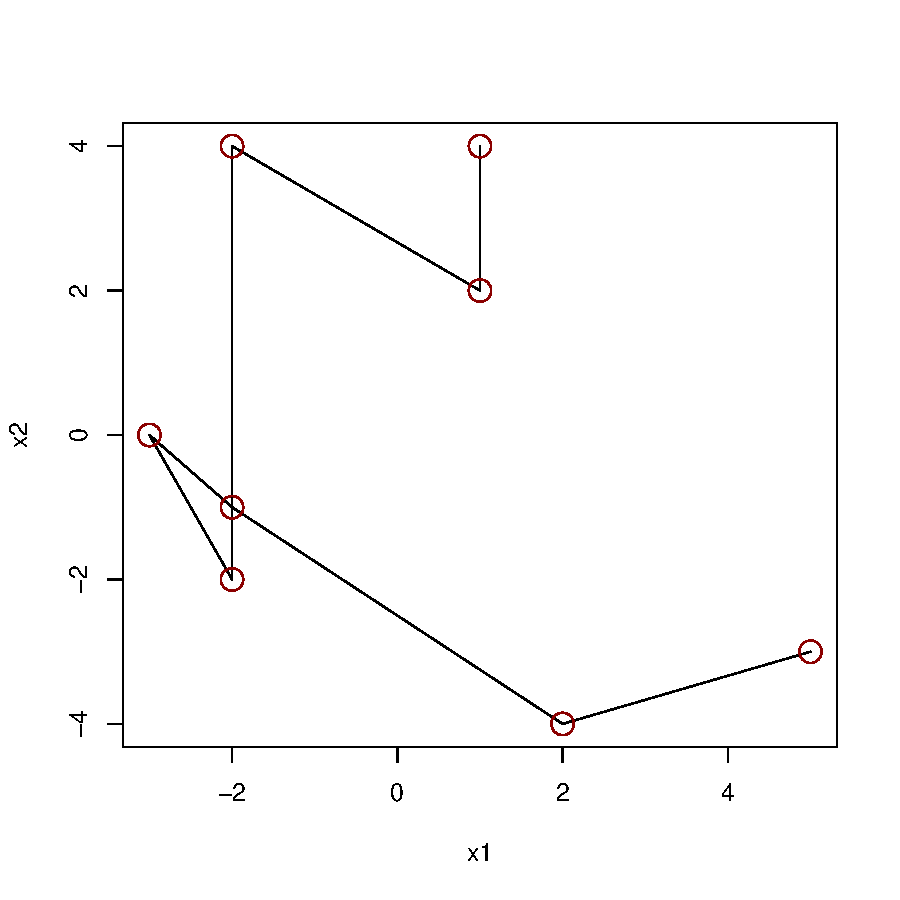
\includegraphics[scale=0.5]{ExCluster1.pdf}}
\end{itemize}
\end{frame}
\begin{frame}
\frametitle{Ejemplo}
\begin{itemize}
\item<2->{La matriz de distancias (distancia euclídea) entre los $8$ puntos es:
$$
D= \begin{pmatrix}
0.00&3.16&7.28&8.54&7.07&9.90&6.40&8.06 \\
&0.00&5.00&6.40&4.47&8.94&6.08&8.06\\
&&0.00&1.41&1.00&5.00&4.24&5.83\\
&&&0.00&2.24&4.12&4.47&5.66\\
&&&&0.00&6.00&5.00&6.71\\
&&&&&0.00&3.61&3.00\\
&&&&&&0.00&2.00\\
&&&&&&&0.00
\end{pmatrix}
$$}
\end{itemize}
\end{frame}
\begin{frame}
\frametitle{Ejemplo}
\begin{itemize}
\item<2->{Aplicación del algoritmo.
Como vemos, los puntos más cercanos son el $3$ y el $5$. Por tanto, los nuevos clústers serán:
$$
\{1\},\ \{2\},\ \{3,5\},\ \{4\},\ \{6\},\ \{7\},\ \{8\}.
$$}
\item<3->{Calculemos la nueva matriz de distancias usando el enlace simple entre los $7$ clústers:
$$
D_2 = 
\begin{pmatrix}
0.00&3.16&7.07&8.54&9.90&6.40&8.06\\
&0.00&4.47&6.40&8.94&6.08&8.06\\
&&0.00&1.41&5.00&4.24&5.83\\
&&&0.00&4.12&4.47&5.66\\
&&&&0.00&3.61&3.00\\
&&&&&0.00&2.00\\
&&&&&&0.00
\end{pmatrix}
$$}
\end{itemize}
\end{frame}
\begin{frame}
\frametitle{Ejemplo}
\begin{itemize}
\item<2->{La distancia más cercana está ahora entre los clústers $\{3,5\}$ y el clúster $\{4\}$. Los nuevos clúster son:
$$
\{1\},\ \{2\},\ \{3,4,5\},\ \{6\},\ \{7\},\ \{8\}.
$$
La nueva matriz de distancias será:
$$
D_3 =
\begin{pmatrix}
0.00&3.16&7.07&9.90&6.40&8.06\\
&0.00&4.47&8.94&6.08&8.06\\
&&0.00&4.12&4.24&5.66\\
&&&0.00&3.61&3.00\\
&&&&0.00&2.00\\
&&&&&0.00
\end{pmatrix}
$$}
\end{itemize}
\end{frame}
\begin{frame}
\frametitle{Ejemplo}
\begin{itemize}
\item<2->{La distancia más cercana se encuentra entre los clústers $\{7\}$ y $\{8\}$. Los nuevos clústers serán:
$$
\{1\},\ \{2\},\ \{3,4,5\},\ \{6\},\ \{7,8\}.
$$
La nueva matriz de distancias será:
$$
D_4 = \begin{pmatrix}
0.00&3.16&7.07&9.90&6.40\\
&0.00&4.47&8.94&6.08\\
&&0.00&4.12&4.24\\
&&&0.00&3.00\\
&&&&0.00
\end{pmatrix}
$$}
\end{itemize}
\end{frame}
\begin{frame}
\frametitle{Ejemplo}
\begin{itemize}
\item<2->{La distancia más cercana se encuentra entre los clústers $\{6\}$ y $\{7,8\}$. Los nuevos clústers serán:
$$
\{1\},\ \{2\},\ \{3,4,5\},\ \{6,7,8\}.
$$
La nueva matriz de distancias será:
$$
D_5= \begin{pmatrix}
0.00&3.16&7.07&6.40\\
&0.00&4.47&6.08\\
&&0.00&4.12\\
&&&0.00
\end{pmatrix}
$$}
\end{itemize}
\end{frame}
\begin{frame}
\frametitle{Ejemplo}
\begin{itemize}
\item<2->{La distancia más cercana se encuentra entre los clústers $\{1\}$ y $\{2\}$. Los nuevos clústers serán:
$$
\{1,2\},\ \{3,4,5\},\ \{6,7,8\}.
$$
La nueva matriz de distancias será:
$$
D_6 = \begin{pmatrix}
0.00 & 4.47 & 6.08\\
& 0.00 & 4.12\\
&&0.00
\end{pmatrix}
$$}
\end{itemize}
\end{frame}
\begin{frame}
\frametitle{Ejemplo}
\begin{itemize}
\item<2->{La distancia más cercana se encuentra entre los clústers $\{3,4,5\}$ y $\{6,7,8\}$. Los nuevos clústers serán:
$$
\{1,2\},\ \{3,4,5,6,7,8\}.
$$
La nueva matriz de distancias será:
$$
D_7 = \begin{pmatrix}
0.00 & 4.47\\
&0.00
\end{pmatrix}
$$}
\item<3->{El último paso del algoritmo será juntar los dos últimos clusters obteniendo un clúster único compuesto por los $8$ puntos.}
\end{itemize}
\end{frame}
\begin{frame}
\frametitle{Ejemplo}
\uncover<2->{Todo el ejemplo queda resumido en lo que se denomina un dendograma:
\vskip 0.05cm
%\includegraphics[scale=0.5]{DendExCluster1.pdf}}
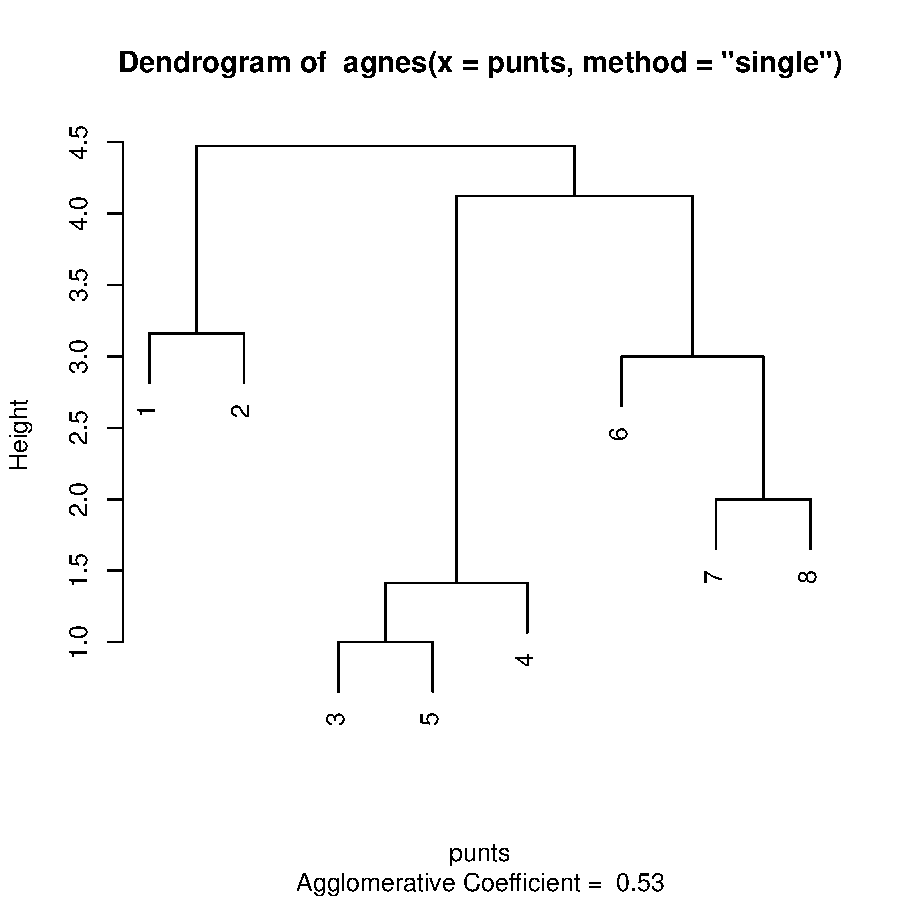
\includegraphics[scale=0.4]{DendogramaPuntsSimple.pdf}}
\end{frame}
\begin{frame}
\frametitle{Propiedades de los algoritmos aglomerativos.}
\begin{itemize}
\item<2->{En el procedimiento del enlace simple, la distancia entre el clúster $R$ y el clúster unión de $P$ y $Q$, $P+Q$ se puede hallar como:
$$
d(R,P+Q)=\min (d(R,P),d(R,Q)).
$$Por dicho motivo, se denomina algoritmo del vecino más próximo. Dicho algoritmo tiende a construir clústers grandes. Clústers que difieren pero que no están bien separados pueden unirse en un sólo clúster si tienen dos individuos próximos.} 
\end{itemize}
\end{frame}
\begin{frame}
\frametitle{Propiedades de los algoritmos aglomerativos.}
\begin{itemize}
\item<2->{En el procedimiento del enlace completo, se trata de corregir este tipo de agrupamiento considerando distancias grandes. De hecho, la distancia entre el clúster $R$ y el clúster unión de $P$ y $Q$, $P+Q$ se puede hallar como:
$$
d(R,P+Q)=\max (d(R,P),d(R,Q)).
$$Por dicho motivo, se denomina el algoritmo del vecino más alejado. Dicho algoritmo agrupa clústers donde todos los puntos están próximos.}
\item<3->{En el procedimiento del enlace promedio, se propone una solución intermedia entre los dos procedimientos anteriores. En este caso, se calcula la distancia promedio:
$$
d(R,P+Q)=\frac{n_P}{n_P + n_Q} d(R,P)+\frac{n_Q}{n_P + n_Q} d(R,Q).
$$}
\end{itemize}
\end{frame}
\begin{frame}
\frametitle{Propiedades de los algoritmos aglomerativos.}
\begin{itemize}
\item<2->{El procedimiento del centroide es similar al procedimiento promedio pero usa la distancia geométrica entre el clúster $R$ y el centro de gravedad promediado entre los clústers $P$ y $Q$.}
\item<3->{El algoritmo de Ward se diferencia de los otros procedimientos respecto de la unificación. Dicho algoritmo no junta grupos con distancias pequeñas sino que junta grupos en los que no se incremente la heterogeneidad de los mismos ``demasiado". El objetivo de dicho procedimiento es que la variación dentro de los clústers no aumente de forma drástica. El resultado es que los grupos son lo más homogéneos posible.}
\end{itemize}
\end{frame}
\begin{frame}
\frametitle{Ejemplo}
\uncover<2->{El dendograma usando el método completo para el ejemplo anterior es:
\vskip 0.05cm
%\includegraphics[scale=0.5]{DendExCluster1.pdf}}
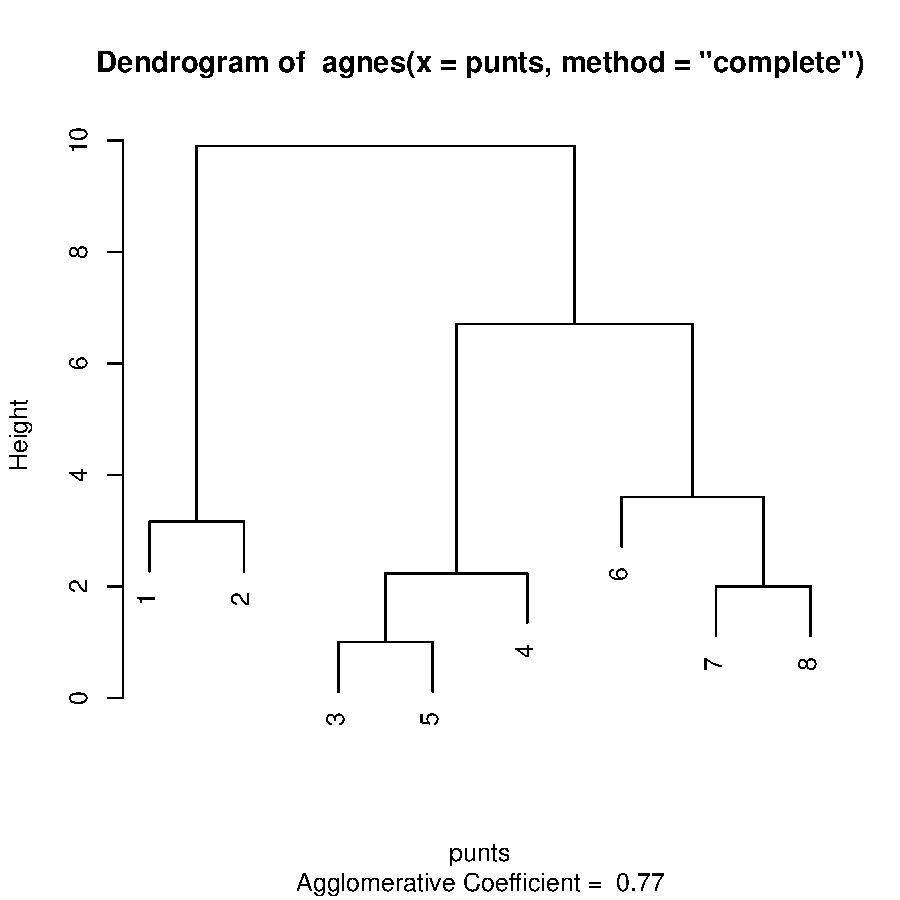
\includegraphics[scale=0.4]{DendogramaPuntsComplet.pdf}}
\end{frame}
\begin{frame}
\frametitle{Ejemplo}
\uncover<2->{El dendograma usando el método promedio para el ejemplo anterior es:
\vskip 0.05cm
%\includegraphics[scale=0.5]{DendExCluster1.pdf}}
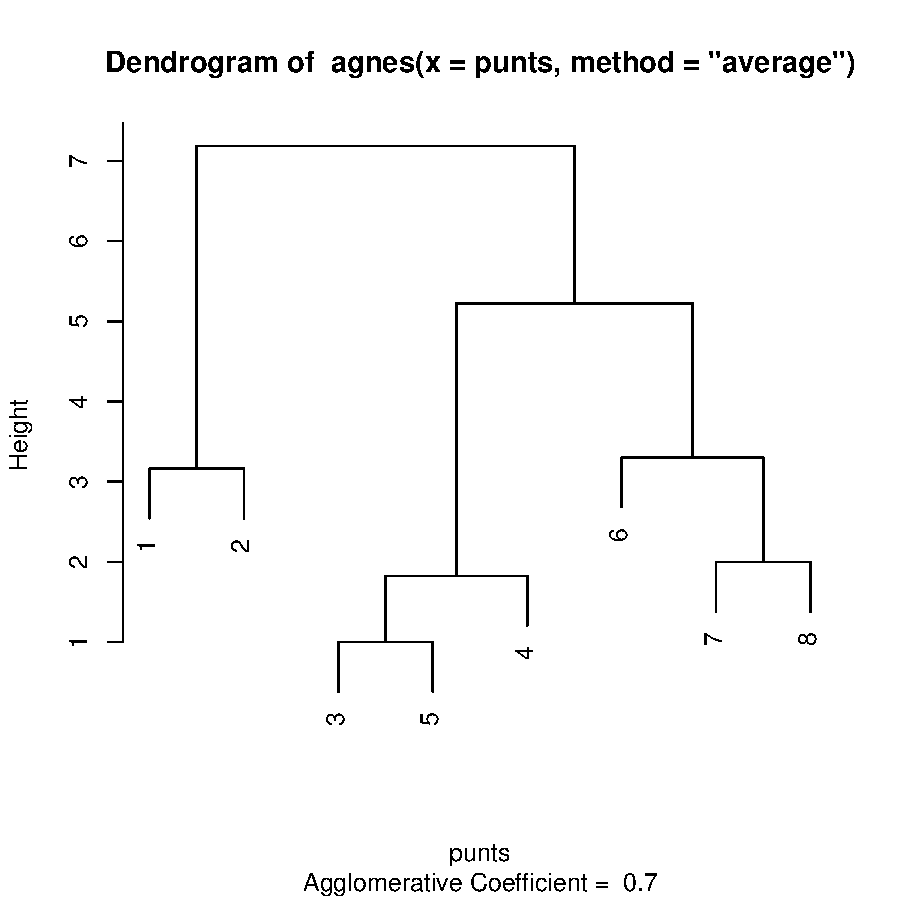
\includegraphics[scale=0.4]{DendogramaPuntsAverage.pdf}}
\end{frame}
\begin{frame}
\frametitle{Ejemplo}
\uncover<2->{El dendograma usando el método de Ward para el ejemplo anterior es:
\vskip 0.05cm
%\includegraphics[scale=0.5]{DendExCluster1.pdf}}
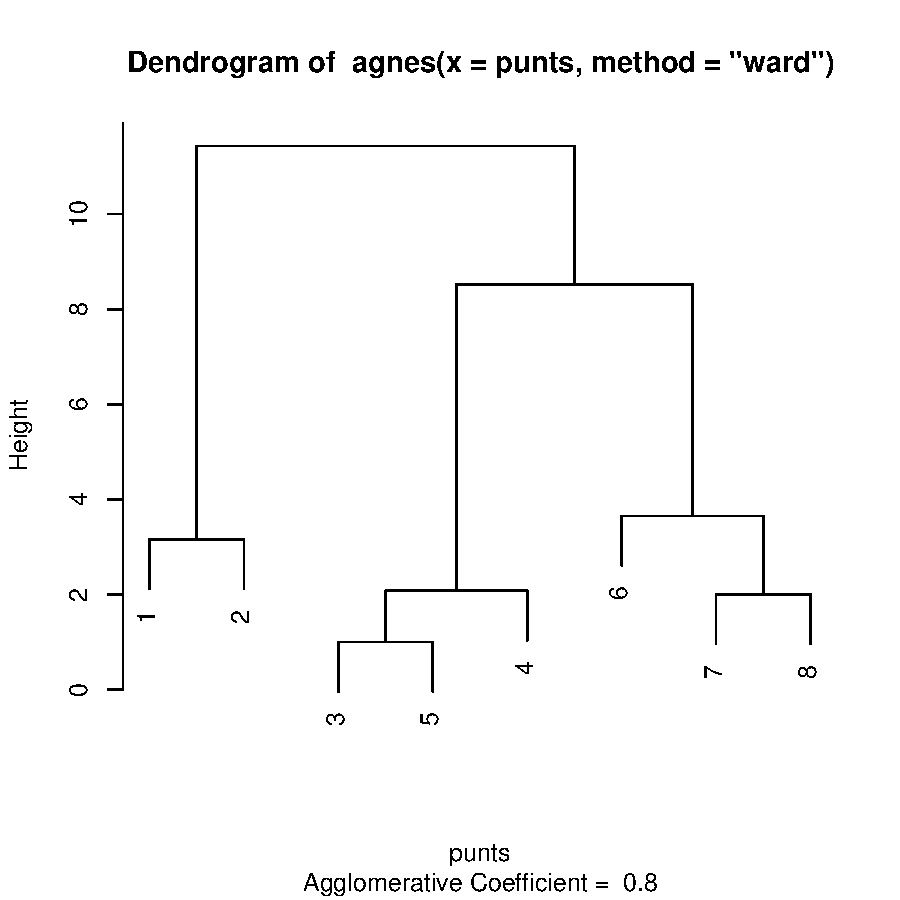
\includegraphics[scale=0.4]{DendogramaPuntsWard.pdf}}
\end{frame}
\begin{frame}
\frametitle{Propiedades de los algoritmos aglomerativos.}
\begin{itemize}
\item<2->{Se define la heterogeneidad de un clúster $R$ como:
$$
I_R = \frac{1}{n_R} \sum_{i=1}^{n_R} d^2(x_i,\overline{x}_R),
$$
donde $\overline{x}_R$ es el centro de gravedad o la media del clúster $R$. Si $d$ es la distancia euclídea, $I_R$ representa la varianza del clúster $R$.}
\item<3->{Cuando dos clústers $P$ y $Q$ se unen, el nuevo clúster $P+Q$ tiene una heterogeneidad $I_{P+Q}$. Puede demostrarse que el aumento de heterogeneidad viene dada por:
$$
\Delta (P,Q)= \frac{n_P n_Q}{n_P + n_Q} d^2 (P,Q).
$$}
\item<4->{El algoritmo de Ward, por tanto, puede definirse como el algoritmo que minimiza $\Delta (P,Q)$.}
\end{itemize}
\end{frame}


\part{Bibliografía}

\frame{\partpage}

\section{Bibliografía}
%\nocite{*}
%\bibliography{biblio}
%\bibliographystyle{plain}




\end{document}
